\appendix

\section{\DatasetName{} Dataset}\label{sec:dataset_appendix}

\begin{table*}[t]
  \small
  \centering
  \setlength{\tabcolsep}{7pt}
  \begin{tabular}{lllll}
    \toprule

    \multicolumn{2}{c}{\textbf{Field}} & \textbf{Patent}                        & \textbf{Paper Candidate 1 (\textcolor{darkgreen}{\checkmark})} & \textbf{Paper Candidate 2 (\textcolor{red}{\ding{55}})}                           \\
    \midrule
    \multirow{2}{*}[-1em]{Authors}
                                       & Content
                                       & Ge Wang, Wenxiang Cong
                                       & \makecell[tl]{Wenxiang Cong, Yan Xi,                                                                                                                                                        \\Bruno De Man, Ge Wang}
                                       & \makecell[tl]{Wenxiang Cong, Yan Xi,                                                                                                                                                        \\Peter Fitzgerald,\\Bruno De Man, Ge Wang}
    \\
                                       & $\text{sim}_\text{author}$             &                                                                & 1.0                                                     & 1.0                     \\
    \cmidrule{1-5}
    \multirow{2}{*}[-2em]{Title}
                                       & Content
                                       & \makecell[tl]{Monochromatic CT Image                                                                                                                                                        \\Reconstruction from Current-\\Integrating Data via Machine Learning}
                                       & \makecell[tl]{Monochromatic image                                                                                                                                                           \\reconstruction via\\machine learning}
                                       & \makecell[tl]{Virtual Monoenergetic                                                                                                                                                         \\CT Imaging via\\Deep Learning}
    \\
                                       & $\text{sim}_\text{term}$               &                                                                & 1.0 / 0.63                                              & 0.39 / 0.32             \\
    \cmidrule{1-5}
    \multirow{2}{*}[-1.5em]{Abstract}
                                       & Content
                                       & \makecell[tl]{A machine-learning-based                                                                                                                                                      \\monochromatic CT image\\reconstruction method is described ...}
                                       & \makecell[tl]{X-ray computed                                                                                                                                                                \\tomography (CT) is a\\ nondestructive imaging ...}
                                       & \makecell[tl]{The physical process                                                                                                                                                          \\of X-ray CT imaging\\is described ...}
    \\
                                       & $\text{sim}_\text{term}$               &                                                                & 0.71 / 0.19                                             & 0.50 / 0.23             \\
    \cmidrule{1-5}
    Date                               &                                        & 2021-08-30                                                     & 2020-11-01 (\checkmark)                                 & 2021-04-14 (\checkmark) \\
    \bottomrule
  \end{tabular}
  \caption{Example for the matching of a PPP. The scores correspond to the respective metrics, the term metrics are shown as $\min$-normalized / $\max$-normalized. Both papers have author lists that contain all the inventors, were published inside the date range, and have titles and abstracts with sufficiently high absolute term similarity to the patent. Since the term similarity scores of paper 1 are higher than those of paper 2 by the specified margin (see Distinctiveness filtering step), paper 1 is correctly matched to the patent.}
  \label{tab:match_example}
\end{table*}

We present the \DatasetName dataset containing 1.8k PPPs from a variety of domains, each annotated with multiple outlines.
It serves two main purposes.
First, it is a challenging benchmark for LLMs that requires long-text generation capabilities and deep understanding of the technical domain as well as patent law. Second, it facilitates the development of AI-powered tools for patent drafting, where the patent attorney only performs post-editing rather than writing from scratch, potentially incurring massive cost savings. In the following, we describe the steps taken for constructing the \DatasetName{} dataset: scraping and filtering PPPs, parsing the full-text documents and generating the patent outlines.

\subsection{Scraping Patent-Paper Pairs}\label{sec:matching}

The patent and paper in a PPP typically do not cite each other, so we cannot rely on front-page or in-text citations \cite{marxRelianceScienceWorldwide2020, marxRelianceScienceInventors2022} to find PPPs. 
The matching must rely on document metadata and content alone. 
We start out with the USPTO dataset\footnote{\url{https://bulkdata.uspto.gov}} containing 6.7M patent applications from 2005 to April 2024.
For each patent, we query SemOpenAlex \cite{farberSemOpenAlexScientificLandscape2023a} using SPARQL and retrieve papers with overlapping authors lists and publication dates.
Next, we filter the results based on their titles, abstracts, other candidate matches for the same patent, and %
paper licenses, as elaborated below. Table \ref{tab:dataset_filters} shows the remaining number of candidates after each filtering step.
As can be seen, the major limiting factor for our benchmark size is the issue of scientific articles being published under restrictive licenses.
An example match is shown in Table \ref{tab:match_example}.
We perform a systematic manual post-hoc evaluation of the heuristics to validate their precision (see Section \ref{sec:validation}).


\noindent\textbf{Author Overlap. } The patent and the paper of a PPP are by definition authored by overlapping sets of individuals. The overlap of author lists have therefore been identified as an effective (yet not sufficient) criteria for matching PPPs \cite{magermanExploringFeasibilityAccuracy2010}.
The requirements for paper authorship are typically much lower than those for patent inventorship \cite{konskiInventorshipAuthorship2015}.
In many cases, only the main author(s) and the senior author(s) are listed as inventors.
We accordingly employ an asymmetric score that only measures the fraction of inventors $i \in I$ that are also authors $a \in A$, not vice versa:
\begin{align*}
  \text{sim}_\text{author} & = \frac{|I \cap A|}{|I|} \geq 0.8
\end{align*}
This score's effectiveness increases with the number of inventors, so we only consider patents with at least two inventors.
Implementing $\text{sim}_\text{author}$ requires some form of author name disambiguation to avoid false negatives (different spellings, e.g., with, without, or with abbreviated middle name) and false positives (e.g., very common names like John Smith).
There are no author identifiers shared between the patent and paper datasets, so our disambiguation uses the surface names only.
To account for false negatives, we use the aliases stored in SemOpenAlex and consider an inventor to be an author if their name matches exactly with one of the aliases.
False positives are marginalized by author combinations and subsequent filters: it is highly unlikely that there exist two groups of people with the same set of names working on the same topic at the same time.

\noindent\textbf{Date Range. } We require the paper's publication date to be within one year before and two years after the patent application date. The former corresponds to the USPTO's grace period,\footnote{\url{https://www.uspto.gov/web/offices/pac/mpep/s2153.html}} which allows inventors to file patent applications up to one year after they disclosed the invention to the public.
The two-year period after the application date was selected because qualitative analyses identified it as the point of diminishing returns, beyond which the incidence of true positives notably decreases, while the rate of false positives significantly increases.

\noindent\textbf{Term Overlap.} We compare titles and abstracts of patents and papers using term overlap metrics.
We first obtain a set of terms $T$ using removal of stopwords and punctuation\footnote{based on spaCy's \texttt{en\_core\_web\_sm}} and stemming.\footnote{based on NLTK's PorterStemmer}
The score is then computed as the number of shared terms, normalized by the minimum or maximum number of terms, following \citet{magermanDoesInvolvementPatenting2015}. We additionally weight each term using its IDF value across all titles and abstracts of patents and papers.
\par\noindent
{
  \small
  \setlength{\abovedisplayskip}{0pt}
  \setlength{\abovedisplayshortskip}{0pt}
  \begin{align*}
    \text{sim}_\text{term}(pat, pap) & = \frac{
      \displaystyle\sum_{t \in T(pat) \cap T(pap)} \text{idf}(t)
    }{
      \displaystyle\text{agg}\Big(\sum_{t \in T(pat)} \text{idf}(t), \sum_{t \in T(pap)} \text{idf}(t)\Big)
    }
  \end{align*}
  \par
}
\noindent where $pat$ and $pap$ are either the titles or the abstracts of the documents, and $\text{agg}\in\{\min, \max\}$.
Thus, we have 4 scores in total, for which we set the thresholds to be 0.15 with $\min$ normalization and 0.1 with $\max$ normalization.
We choose the values based on interactive experimentation, but perform a post-hoc validation of the matching precision.

\noindent\textbf{Distinctiveness. }
In the remaining candidate pairs, there are still many cases where one patent is matched to multiple papers or vice versa. We disambiguate these cases by comparing the term overlap metrics among these ambiguous candidate groups. We only keep a pair if 3 out of 4 term metrics are higher than those of any other candidate in the group by a margin of 0.15 and 0.1, for $\min$ and $\max$, respectively.

\noindent\textbf{License. } We filter the matches for licenses that allow redistribution and commercial use, i.e., 
CC-BY,%
CC0,%
and public domain.
We use the license information provided by SemOpenAlex and by the ArXiv API.

\subsection{Manual Validation}\label{sec:validation}

To verify the precision of our matching pipeline, we perform a manual validation, conducted by the first author of this paper.
We randomly sample 60 PPPs, read both abstracts, skim the documents, compare the figures and get an overview of the authors' related work. We spend roughly 5 minutes per pair on average.
We find that in 55/60 ($91.7\%$) pairs, the paper indeed describes the invention as one of the core contributions.
In three pairs, the best match for the patent would have been a prior paper by the same authors.
In two pairs, the paper would have been best matched to a related but different patent by the same inventors.
This result validates the precision of our matching approach.
In the five imperfect matching cases, the papers still provide meaningful training and evaluation signals, as they are still closely related to the invention and contextualized by the outline.

\subsection{Document Parsing}

We parse all patents and papers into a nested JSON schema where each section has a title, paragraphs and subsections field. We make considerable efforts to obtain clean data: we perform LLM-based section hierarchy reconstruction for patents, font-based section hierarchy reconstruction for paper PDFs and formula conversion for patents and papers. We provide more details in Appendix \ref{sec:parsing_appendix}.


\subsection{Dataset Characteristics}

We split our dataset randomly into \textit{train} (n=1000), \textit{test} (n=500) and \textit{validation} (n=242). We additionally create a non-contaminated test set (\textit{nc-test}) that contains all pairs with a patent published in 2024 (n=71), i.e., after the pretraining cut-off date of all evaluated open-weight LLMs. 
Thus, we address the concern that LLMs might have seen test data during pretraining \cite{ravaut2024much}.
Table \ref{tab:dataset_stats} shows dataset statistics across the splits. Appendix \ref{sec:dataset_stats_appendix} shows further statistics and plots, including the distribution over domains and the number of pairs over time.

In general, both patents and papers contain information not present in the other.
The paper typically includes more experimental details and insights drawn from the experiments.
The patent usually contains more information on the applications and practical benefits of the invention.
We analyze the lexical overlaps between the documents and find that only 2.1\% of the 4-grams are shared.
This underlines the complexity of the task: the two documents describe the same invention from a different perspective using different language.
Nevertheless, we find that it is common for attorneys to copy content from the paper to the patent (or vice versa). 
For instance, many patents and papers share a portion of the figures, as well as verbatim copied text.



\FloatBarrier
\section{Document Parsing Pipeline}\label{sec:parsing_appendix}
\FloatBarrier

In total, we use three different data sources for the full texts.
For the patents, we use the USPTO bulk downloads\footnote{\url{https://bulkdata.uspto.gov/}}.
For the papers, we use PubMed if available and PDF otherwise.
The goal is to extract a clean representation of the full text into a common JSON format.
In this format, every section has a title, a list of paragraphs and a list of subsections.
We write parsers for the XML formats from USPTO, PubMed and the PDF parser Grobid\footnote{\url{https://github.com/kermitt2/grobid}}.
In addition, we perform several cleaning steps:\begin{enumerate}
  \item \textbf{PDF Hierarchy Reconstruction. } The JSON format is hierarchical by nature,  for instance to enable better chunking of patents and section-based retrieval from papers. However, Grobid does not detect section levels if the sections are not numbered. To reconstruct the levels in these cases, we implement a solution that searches for the headings in the PDF file, extracts their font properties, orders them by size, boldness and capitalization, and infers the levels from that.
  \item \textbf{Patent Hierarchy Reconstruction. } In USPTO's patent XML files, there is a level attribute associated with every heading, but we find that it is rarely correct; most headings are placed on the same level. To reconstruct the levels, we pass the list of headings to an LLM and instruct it to infer the levels based on their names (e.g., "Example 1" and "Example 2" and likely children of "EXAMPLES").
  \item \textbf{Formula Conversion. } Many patents and papers include formulas that can be an important part of the document. However, in USPTO's and PubMed's XML formats, formulas are represented in MathML syntax, which is extremely hard to read and arguably hard to generate. To that end, we convert all MathML formulas to latex using pandoc\footnote{\url{https://github.com/jgm/pandoc}}.
  \item \textbf{Metadata Section Filtering. } Patents usually contain a number of metadata sections in the full text, such as information regarding funding or cross-references to related patents. To filter out these sections, we collect a list of such heading names and remove a section if its heading has a Levenshtein distance less than 3 to any one of the blacklisted headings.
\end{enumerate}



\FloatBarrier
\clearpage
\section{Repetition Removal}\label{sec:rep_removal}
\FloatBarrier

\begin{algorithm*}[ht!]
  \small
  \caption{Repetition Detection}
  \label{alg:rep_removal}
  \begin{algorithmic}[1]
    \Function{matches}{l1, l2}
      \State $n\_match \gets 0$
      \For{$i \gets 0$ \textbf{to} $\text{len}(l1) - 1$}
        \If{$l1[i] = l2[i$]}
          \State $n\_match \gets n\_match + 1$
        \EndIf
      \EndFor
      \State \Return n\_match / len(l1) $>$ 0.9
    \EndFunction
    \\
    \Function{detect\_repetitions}{words, min\_length, max\_cycle\_length}
        \State $n \gets len(words)$
        \For{$k = 1$ to max\_cycle\_length}
            \If{matches(words[-k:], words[-2 * k : -k])} \Comment{Check for repetition of length k}
                \State $i \gets 2$ \Comment{Number of times the pattern is repeated}
                \While{matches(words[-k:], words[-(i + 1) * k : -i * k])} \Comment{Search for additional occurrences}
                    \State $i \gets i + 1$
                \EndWhile
                
                \State remove\_indices $\gets$ [n - (i - 1) * k, ..., n]
                \State total\_length $\gets i * k$

                \If{total\_length $\ge$ min\_length}
                    \State words $\gets$ words[: n - (i - 1) * k]  \Comment{Keep only first occurrence of pattern}
                    \State remove\_rest $\gets$ detect\_repetitions(words, min\_length, max\_cycle\_length) \Comment{Recursive call for remaining text}
                    \State \Return remove\_indices + remove\_rest \Comment{Return indices to remove}
                \EndIf
            \EndIf
        \EndFor
        \State \Return []
    \EndFunction
  \end{algorithmic}
\end{algorithm*}
\FloatBarrier
We design a procedure to remove infinite repetitions from generated outputs to study their effect on evaluation metrics.  
In that context, we characterize an infinite repetition as a sequence of tokens that appears multiple times until the end of the generation.  
To find such repetitions, we apply the following recursive algorithm in \Cref{alg:rep_removal} to each chunk and remove the returned indices.
To account for reptitions where the model alters the patterns slightly (e.g., incrementing a number) in each iteration, we consider two word sequences equal if 90\% of their positions are equal.
By default, we use min\_length = 50 and max\_cycle\_length = 300. 

\FloatBarrier
\section{Contamination Results}\label{sec:nc-test-results}
\FloatBarrier


\begin{table*}[t]
    \centering
    \small
    \resizebox{\textwidth}{!}{
      \setlength{\tabcolsep}{3pt}
      \begin{tabular}{lccccccccccc}
        \toprule
                              & \multirow{4}{*}{Tokens}
                              & \multicolumn{2}{c}{\multirow{3}{*}{Text Sim $\uparrow$}}
                              & \multicolumn{3}{c}{Content-Level Metrics (SCALE) $\uparrow$}
                              & \multicolumn{2}{c}{\multirow{3}{*}{Language $\uparrow$}}
                              & \multicolumn{2}{c}{\multirow{3}{*}{Repetitions}}
        \\
        \cmidrule(lr){5-7}
                              &
                              &
                              &
                              & Coverage
                              & \multicolumn{2}{c}{Factuality}
                              &
                              &
                              &
                              &
                              &
        \\
        \cmidrule(lr){3-4}\cmidrule(lr){6-7}\cmidrule(lr){8-9}\cmidrule(lr){10-11}
                              &
                              & BS
                              & R-L
                              & \textit{Gen} \textrightarrow{} \textit{Ref}
                              & \textit{Ref} \textrightarrow{} \textit{Gen}
                              & \textit{Ref} + \textit{Pap} \textrightarrow{} \textit{Gen}
                              & Style
                              & DiscoScore
                              & RR
                              & RR>80
        \\
        \midrule
    
        \multicolumn{8}{l}{\textbf{Heuristic Baselines / Skylines}}\vspace{.4em}                                                                                                      \\
        Reference Patent
                              & \textit{18.4k (100.0\%)}
                              & \textit{100.0}
                              & \textit{100.0}
                              & \textit{88.6 $\pm$ .57}
                              & \textit{88.5 $\pm$ .23}
                              & \textit{88.7 $\pm$ .21}
                              & \textit{99.8}
                              & \textit{100.0}
                              & 15.2
                              & 0.1
        \\
        Similar Patent
                              & 26.1k (141.8\%)
                              & 66.0
                              & 35.3
                              & 31.4 $\pm$ .93
                              & 28.0 $\pm$ .64
                              & 28.3 $\pm$ .68
                              & 53.9
                              & 98.1
                              & 12.5
                              & 0.1
        \\
        Outline
                              & 1.4k (7.6\%)
                              & 56.7
                              & 10.2
                              & 42.1 $\pm$ .94
                              & 63.4 $\pm$ .88
                              & 63.8 $\pm$ .86
                              & 25.9
                              & 85.1
                              & 19.4
                              & 0.0
        \\
        Paper
                              & 9.5k (51.7\%)
                              & 69.6
                              & 42.2
                              & 46.7 $\pm$ 1.01
                              & 46.5 $\pm$ .87
                              & \textit{88.8 $\pm$ .41}
                              & 37.2
                              & 98.0
                              & 8.2
                              & 0.0
        \\
        \cmidrule{1-11}
        \multicolumn{8}{l}{\textbf{Single LLM-call} ($\mathcal{T}$\textit{$\{$inst=2k; pap=$\infty$; pat=$\infty\}$})}\vspace{.4em}                                                                                                          \\
        Mixtral-8x7B
                              & 3.0k (16.3\%)
                              & \textbf{\itshape 66.5}
                              & 21.7
                              & 40.7 $\pm$ 1.16
                              & \textbf{67.2 }$\pm$ 1.19
                              & 73.9 $\pm$ 1.16
                              & \textbf{\itshape 36.5}
                              & 96.8
                              & 15.9
                              & 0.1
        \\
        Qwen2-72B
                              & 2.9k (15.5\%)
                              & 66.4
                              & 21.2
                              & \textbf{\itshape 42.0 }$\pm$ 1.21
                              & 65.0 $\pm$ .76
                              & 71.9 $\pm$ .23
                              & 34.5
                              & \textbf{\itshape 96.9}
                              & \textbf{8.9}
                              & \textbf{0.0}
        \\
        $\quad$w/o Paper
                              & 3.4k (18.2\%)
                              & 65.9
                              & \textbf{\itshape 21.8}
                              & 41.4 $\pm$ 1.25
                              & 66.3 $\pm$ 1.04
                              & 67.0 $\pm$ .99
                              & 34.1
                              & 96.1
                              & 9.0
                              & 0.2
        \\
        $\quad$w/o Outline
                              & 2.0k (11.0\%)
                              & 63.7
                              & 15.8
                              & 36.7 $\pm$ 1.27
                              & 56.5 $\pm$ .67
                              & \textbf{75.7 }$\pm$ 1.13
                              & 30.3
                              & 96.8
                              & \textbf{\itshape 8.2}
                              & \textbf{0.0}
        \\
    
        \cmidrule{1-11}
        \multicolumn{8}{l}{\textbf{\MethodName} ($\mathcal{T}$\textit{$\{$inst=2k; pap=3k; pat=2k$\}$})}\vspace{.4em}                                                                                \\
        Llama-3 8B
                              & 9.6k (52.1\%)
                              & 68.8
                              & 41.4
                              & 42.3 $\pm$ 1.11
                              & 60.3 $\pm$ 1.60
                              & 65.6 $\pm$ 1.23
                              & 36.8
                              & 96.6
                              & 25.4
                              & 2.7
        \\
        Llama-3 8B SFT
                              & 27.0k (146.8\%)
                              & 71.2
                              & 44.0
                              & 44.0 $\pm$ 1.47
                              & 49.4 $\pm$ 1.42
                              & 52.1 $\pm$ 1.36
                              & 45.0
                              & 97.8
                              & 53.7
                              & 27.6
        \\
        $\quad$w/ rep. removal
                              & 18.2k (99.1\%)
                              & \textbf{\itshape 72.1}
                              & \textbf{51.1}
                              & 44.7 $\pm$ 1.03
                              & 52.0 $\pm$ 1.13
                              & 55.4 $\pm$ 1.15
                              & \textbf{50.7}
                              & \textbf{98.2}
                              & 39.6
                              & 8.3
        \\
        Mixtral-8x7B
                              & 6.3k (34.4\%)
                              & 68.8
                              & 34.4
                              & 45.1 $\pm$ 2.00
                              & 64.4 $\pm$ 1.40
                              & \textbf{\itshape 70.6 }$\pm$ 1.24
                              & 39.5
                              & 96.9
                              & 14.4
                              & 0.1
        \\
        Llama-3 70B
                              & 6.1k (33.4\%)
                              & 70.5
                              & 39.5
                              & 45.9 $\pm$ 1.15
                              & 64.7 $\pm$ 1.06
                              & 68.7 $\pm$ .87
                              & 44.6
                              & 97.0
                              & 17.2
                              & 0.1
        \\
        Qwen2-72B
                              & 8.2k (44.7\%)
                              & 70.4
                              & 40.1
                              & \textbf{\itshape 46.9 }$\pm$ 1.26
                              & \textbf{\itshape 65.3 }$\pm$ .83
                              & 69.8 $\pm$ .42
                              & 44.3
                              & 97.0
                              & \textbf{\itshape 10.9}
                              & \textbf{0.0}
        \\
        \cmidrule{1-11}
        \multicolumn{8}{l}{\textbf{\MethodName} ($\mathcal{T}$\textit{$\{$inst=2k; pap=3k; pat=400$\}$})}\vspace{.4em}                                                                                    \\
        Qwen2-72B
                              & 17.2k (93.2\%)
                              & \textbf{\itshape 71.5}
                              & \textbf{\itshape 50.5}
                              & \textbf{49.9 }$\pm$ 1.70
                              & 59.2 $\pm$ 1.00
                              & 64.9 $\pm$ .43
                              & 41.9
                              & 96.6
                              & 8.8
                              & 0.2
        \\
        \bottomrule
    \end{tabular}
    
    }
    \caption{
      Experimental Results on the non-contaminated test set. 
      \textit{Italic values} represent upper bounds that used test data in the prediction. 
      The best value per column is \textbf{bold}, the best per section \textbf{\itshape bold italics}.
      Tokens are reported as absolute and relative to the reference.
      BS = BERTScore. R-L = ROUGE-L. Text Sim = Standard Text Similarity Metrics.
    }
    \label{tab:results-nc-test}
\end{table*}
  


\FloatBarrier
\renewcommand{\sparqlbasicstyle}{\tiny\tt}
\begin{figure*}
  \section{Patent Outline Example}\label{sec:patent_outline_appendix}
  \begin{minipage}{\textwidth}
  \centering
  \lstinputlisting[language=markdown, style=markdownstyle, caption={Example patent outline (short variant) for the pair W6364285-US20140112582. The outline corresponds to more than 5 pages. This example was randomly selected.}]{sections/outline_example.txt}
\end{minipage}
\end{figure*}
\renewcommand{\sparqlbasicstyle}{\small\tt}


\FloatBarrier



\begin{figure*}
  \section{Patent Structure}\label{sec:patent_structure_appendix}
  \begin{minipage}{\textwidth}
  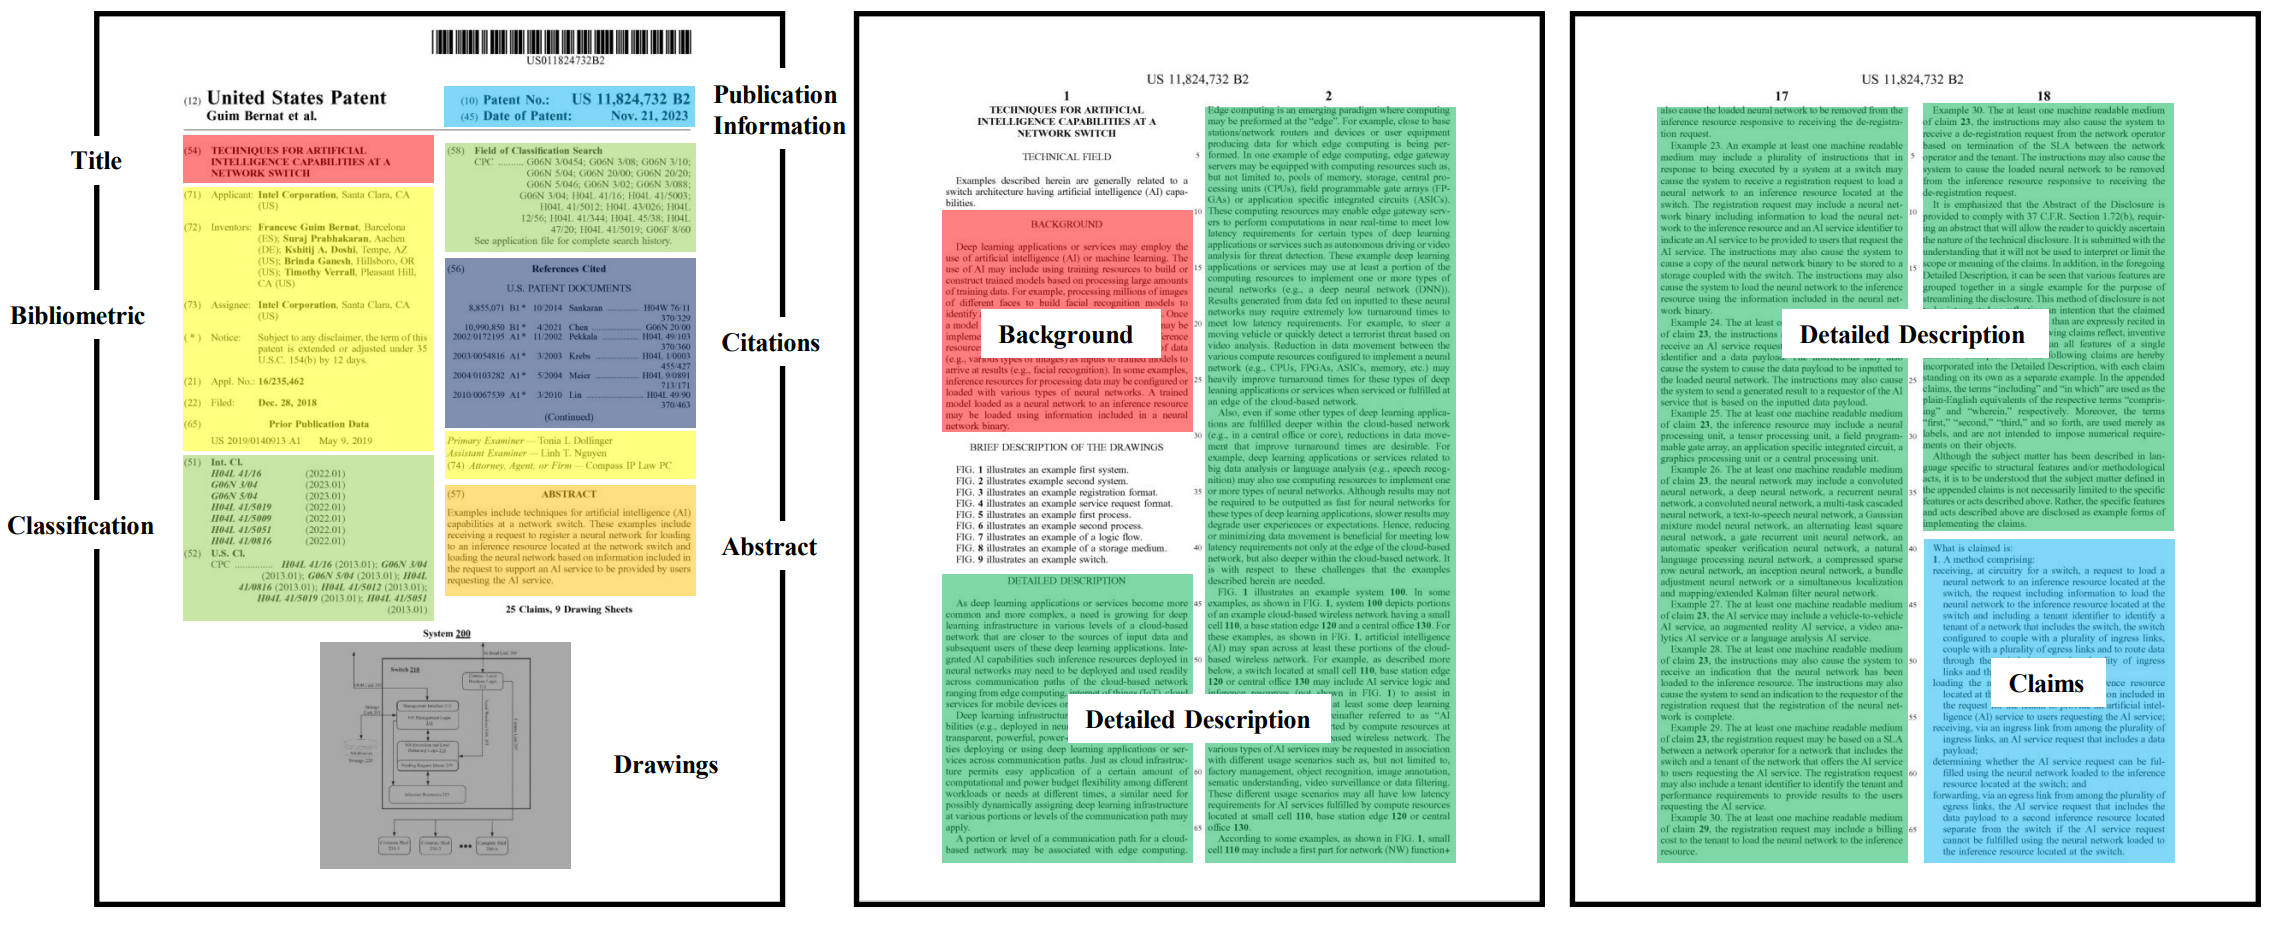
\includegraphics[width=\linewidth]{img/patent.png}
  \caption{Illustration of the structure of a patent from \citet{jiangArtificialIntelligenceExploring2024}. Note that multiple pages from the detailed description are omitted. The description includes all sections except the front matter and claims. In our experiments, we exclude sections containing only metadata, such as statements regarding funding.}
\end{minipage}
\end{figure*}


\FloatBarrier


\begin{table*}
\begin{minipage}{\textwidth}
  \section{Hyperparameters}\label{sec:hyperparameter_appendix}
  \centering
  \begin{tabular}{llcll}
    \toprule
    \multicolumn{2}{c}{Generation} &       & \multicolumn{2}{c}{Training}                                    \\
    \cmidrule{1-2}\cmidrule{4-5}
    Parameter                      & Value &                              & Parameter           & Value      \\
    \midrule
    max sequence length            & 8192  &                              & max sequence length & 8192       \\
    temperature                    & 0.6   &                              & learning rate       & 0.00031622 \\
                                   &       &                              & scheduler           & cosine     \\
                                   &       &                              & warmup ratio        & 0.1        \\
                                   &       &                              & epochs              & 3          \\
                                   &       &                              & batch size          & 32         \\
                                   &       &                              & lora alpha          & 60         \\
                                   &       &                              & lora dropout        & 0.05       \\
                                   &       &                              & lora r              & 128        \\
    \bottomrule
  \end{tabular}
  \caption{Hyperparameters during generation and training. Training parameters are adopted from \citet{tribesHyperparameterOptimizationLarge2024}. We run the experiments on Nvidia H100 80GB GPUs. We use a single H100 for inference and training of the 8B model and 4xH100 for the inference of the larger models using tensor parallel. We estimate the total number of GPU-hours to be 720.}
\end{minipage}
\end{table*}


\FloatBarrier


\renewcommand{\sparqlbasicstyle}{\tiny\tt}
\begin{figure*}
  \section{SPARQL Query}\label{sec:sparql_appendix}
  \begin{minipage}{\textwidth}
  \centering
  \lstinputlisting[language=SPARQL, style=sparqlstyle, caption={SPARQL query template used to retrieve papers for a given patent from SemOpenAlex. Template variables \texttt{<var>} are filled based on the query patent.}]{sections/sparql_query.txt}
\end{minipage}
\end{figure*}
\renewcommand{\sparqlbasicstyle}{\small\tt}


\FloatBarrier


\renewcommand{\sparqlbasicstyle}{\tiny\tt}
\begin{figure*}
  \section{Summary Generation Prompt}\label{sec:summary_prompt_appendix}
  \begin{minipage}{\textwidth}
  \centering
  \lstinputlisting[language=SPARQL, style=sparqlstyle, caption={Prompt used to generate bullet point summaries with Llama-3 70B}]{sections/summary_prompt.txt}
\end{minipage}
\end{figure*}
\renewcommand{\sparqlbasicstyle}{\small\tt}

\FloatBarrier


\renewcommand{\sparqlbasicstyle}{\tiny\tt}
\begin{figure*}
  \section{Patent Generation Prompt}\label{sec:generation_prompt_appendix}
  \begin{minipage}{\textwidth}
  \centering
  \lstinputlisting[language=SPARQL, style=sparqlstyle, caption={System prompt used for outline-guided paper-to-patent generation}]{sections/generation_prompt_system.txt}
\end{minipage}
\end{figure*}

\FloatBarrier


\begin{figure*}
\begin{minipage}{\textwidth}
  \centering
  \lstinputlisting[language=SPARQL, style=sparqlstyle, caption={User prompt used for outline-guided paper-to-patent generation (Part 1)}]{sections/generation_prompt_user_0.txt}
\end{minipage}
\end{figure*}

\begin{figure*}
\begin{minipage}{\textwidth}
  \centering
  \lstinputlisting[language=SPARQL, style=sparqlstyle, caption={User prompt used for outline-guided paper-to-patent generation (Part 2)}]{sections/generation_prompt_user_1.txt}
\end{minipage}
\end{figure*}

\begin{figure*}
\begin{minipage}{\textwidth}
  \centering
  \lstinputlisting[language=SPARQL, style=sparqlstyle, caption={User prompt used for outline-guided paper-to-patent generation (Part 3)}]{sections/generation_prompt_user_2.txt}
\end{minipage}
\end{figure*}

\begin{figure*}
\begin{minipage}{\textwidth}
  \centering
  \lstinputlisting[language=SPARQL, style=sparqlstyle, caption={User prompt used for outline-guided paper-to-patent generation (Part 4)}]{sections/generation_prompt_user_3.txt}
\end{minipage}
\end{figure*}

\renewcommand{\sparqlbasicstyle}{\small\tt}


\FloatBarrier

\begin{figure*}[!ht]
  \section{Dataset Statistics}\label{sec:dataset_stats_appendix}
  \begin{minipage}{\textwidth}
  \centering
  %% Creator: Matplotlib, PGF backend
%%
%% To include the figure in your LaTeX document, write
%%   \input{<filename>.pgf}
%%
%% Make sure the required packages are loaded in your preamble
%%   \usepackage{pgf}
%%
%% Also ensure that all the required font packages are loaded; for instance,
%% the lmodern package is sometimes necessary when using math font.
%%   \usepackage{lmodern}
%%
%% Figures using additional raster images can only be included by \input if
%% they are in the same directory as the main LaTeX file. For loading figures
%% from other directories you can use the `import` package
%%   \usepackage{import}
%%
%% and then include the figures with
%%   \import{<path to file>}{<filename>.pgf}
%%
%% Matplotlib used the following preamble
%%   \def\mathdefault#1{#1}
%%   \everymath=\expandafter{\the\everymath\displaystyle}
%%   
%%   \makeatletter\@ifpackageloaded{underscore}{}{\usepackage[strings]{underscore}}\makeatother
%%
\begingroup%
\makeatletter%
\begin{pgfpicture}%
\pgfpathrectangle{\pgfpointorigin}{\pgfqpoint{5.599828in}{2.000965in}}%
\pgfusepath{use as bounding box, clip}%
\begin{pgfscope}%
\pgfsetbuttcap%
\pgfsetmiterjoin%
\definecolor{currentfill}{rgb}{1.000000,1.000000,1.000000}%
\pgfsetfillcolor{currentfill}%
\pgfsetlinewidth{0.000000pt}%
\definecolor{currentstroke}{rgb}{0.500000,0.500000,0.500000}%
\pgfsetstrokecolor{currentstroke}%
\pgfsetdash{}{0pt}%
\pgfpathmoveto{\pgfqpoint{0.000000in}{0.000000in}}%
\pgfpathlineto{\pgfqpoint{5.599828in}{0.000000in}}%
\pgfpathlineto{\pgfqpoint{5.599828in}{2.000965in}}%
\pgfpathlineto{\pgfqpoint{0.000000in}{2.000965in}}%
\pgfpathlineto{\pgfqpoint{0.000000in}{0.000000in}}%
\pgfpathclose%
\pgfusepath{fill}%
\end{pgfscope}%
\begin{pgfscope}%
\pgfsetbuttcap%
\pgfsetmiterjoin%
\definecolor{currentfill}{rgb}{0.898039,0.898039,0.898039}%
\pgfsetfillcolor{currentfill}%
\pgfsetlinewidth{0.000000pt}%
\definecolor{currentstroke}{rgb}{0.000000,0.000000,0.000000}%
\pgfsetstrokecolor{currentstroke}%
\pgfsetstrokeopacity{0.000000}%
\pgfsetdash{}{0pt}%
\pgfpathmoveto{\pgfqpoint{0.340934in}{0.805783in}}%
\pgfpathlineto{\pgfqpoint{1.349110in}{0.805783in}}%
\pgfpathlineto{\pgfqpoint{1.349110in}{1.730826in}}%
\pgfpathlineto{\pgfqpoint{0.340934in}{1.730826in}}%
\pgfpathlineto{\pgfqpoint{0.340934in}{0.805783in}}%
\pgfpathclose%
\pgfusepath{fill}%
\end{pgfscope}%
\begin{pgfscope}%
\pgfpathrectangle{\pgfqpoint{0.340934in}{0.805783in}}{\pgfqpoint{1.008176in}{0.925043in}}%
\pgfusepath{clip}%
\pgfsetrectcap%
\pgfsetroundjoin%
\pgfsetlinewidth{0.803000pt}%
\definecolor{currentstroke}{rgb}{1.000000,1.000000,1.000000}%
\pgfsetstrokecolor{currentstroke}%
\pgfsetdash{}{0pt}%
\pgfpathmoveto{\pgfqpoint{0.340934in}{0.805783in}}%
\pgfpathlineto{\pgfqpoint{1.349110in}{0.805783in}}%
\pgfusepath{stroke}%
\end{pgfscope}%
\begin{pgfscope}%
\pgfsetbuttcap%
\pgfsetroundjoin%
\definecolor{currentfill}{rgb}{0.333333,0.333333,0.333333}%
\pgfsetfillcolor{currentfill}%
\pgfsetlinewidth{0.803000pt}%
\definecolor{currentstroke}{rgb}{0.333333,0.333333,0.333333}%
\pgfsetstrokecolor{currentstroke}%
\pgfsetdash{}{0pt}%
\pgfsys@defobject{currentmarker}{\pgfqpoint{-0.048611in}{0.000000in}}{\pgfqpoint{-0.000000in}{0.000000in}}{%
\pgfpathmoveto{\pgfqpoint{-0.000000in}{0.000000in}}%
\pgfpathlineto{\pgfqpoint{-0.048611in}{0.000000in}}%
\pgfusepath{stroke,fill}%
}%
\begin{pgfscope}%
\pgfsys@transformshift{0.340934in}{0.805783in}%
\pgfsys@useobject{currentmarker}{}%
\end{pgfscope}%
\end{pgfscope}%
\begin{pgfscope}%
\definecolor{textcolor}{rgb}{0.333333,0.333333,0.333333}%
\pgfsetstrokecolor{textcolor}%
\pgfsetfillcolor{textcolor}%
\pgftext[x=0.100000in, y=0.772025in, left, base]{\color{textcolor}{\rmfamily\fontsize{7.000000}{8.400000}\selectfont\catcode`\^=\active\def^{\ifmmode\sp\else\^{}\fi}\catcode`\%=\active\def%{\%}$\mathdefault{0.0}$}}%
\end{pgfscope}%
\begin{pgfscope}%
\pgfpathrectangle{\pgfqpoint{0.340934in}{0.805783in}}{\pgfqpoint{1.008176in}{0.925043in}}%
\pgfusepath{clip}%
\pgfsetrectcap%
\pgfsetroundjoin%
\pgfsetlinewidth{0.803000pt}%
\definecolor{currentstroke}{rgb}{1.000000,1.000000,1.000000}%
\pgfsetstrokecolor{currentstroke}%
\pgfsetdash{}{0pt}%
\pgfpathmoveto{\pgfqpoint{0.340934in}{1.125151in}}%
\pgfpathlineto{\pgfqpoint{1.349110in}{1.125151in}}%
\pgfusepath{stroke}%
\end{pgfscope}%
\begin{pgfscope}%
\pgfsetbuttcap%
\pgfsetroundjoin%
\definecolor{currentfill}{rgb}{0.333333,0.333333,0.333333}%
\pgfsetfillcolor{currentfill}%
\pgfsetlinewidth{0.803000pt}%
\definecolor{currentstroke}{rgb}{0.333333,0.333333,0.333333}%
\pgfsetstrokecolor{currentstroke}%
\pgfsetdash{}{0pt}%
\pgfsys@defobject{currentmarker}{\pgfqpoint{-0.048611in}{0.000000in}}{\pgfqpoint{-0.000000in}{0.000000in}}{%
\pgfpathmoveto{\pgfqpoint{-0.000000in}{0.000000in}}%
\pgfpathlineto{\pgfqpoint{-0.048611in}{0.000000in}}%
\pgfusepath{stroke,fill}%
}%
\begin{pgfscope}%
\pgfsys@transformshift{0.340934in}{1.125151in}%
\pgfsys@useobject{currentmarker}{}%
\end{pgfscope}%
\end{pgfscope}%
\begin{pgfscope}%
\definecolor{textcolor}{rgb}{0.333333,0.333333,0.333333}%
\pgfsetstrokecolor{textcolor}%
\pgfsetfillcolor{textcolor}%
\pgftext[x=0.100000in, y=1.091394in, left, base]{\color{textcolor}{\rmfamily\fontsize{7.000000}{8.400000}\selectfont\catcode`\^=\active\def^{\ifmmode\sp\else\^{}\fi}\catcode`\%=\active\def%{\%}$\mathdefault{0.2}$}}%
\end{pgfscope}%
\begin{pgfscope}%
\pgfpathrectangle{\pgfqpoint{0.340934in}{0.805783in}}{\pgfqpoint{1.008176in}{0.925043in}}%
\pgfusepath{clip}%
\pgfsetrectcap%
\pgfsetroundjoin%
\pgfsetlinewidth{0.803000pt}%
\definecolor{currentstroke}{rgb}{1.000000,1.000000,1.000000}%
\pgfsetstrokecolor{currentstroke}%
\pgfsetdash{}{0pt}%
\pgfpathmoveto{\pgfqpoint{0.340934in}{1.444519in}}%
\pgfpathlineto{\pgfqpoint{1.349110in}{1.444519in}}%
\pgfusepath{stroke}%
\end{pgfscope}%
\begin{pgfscope}%
\pgfsetbuttcap%
\pgfsetroundjoin%
\definecolor{currentfill}{rgb}{0.333333,0.333333,0.333333}%
\pgfsetfillcolor{currentfill}%
\pgfsetlinewidth{0.803000pt}%
\definecolor{currentstroke}{rgb}{0.333333,0.333333,0.333333}%
\pgfsetstrokecolor{currentstroke}%
\pgfsetdash{}{0pt}%
\pgfsys@defobject{currentmarker}{\pgfqpoint{-0.048611in}{0.000000in}}{\pgfqpoint{-0.000000in}{0.000000in}}{%
\pgfpathmoveto{\pgfqpoint{-0.000000in}{0.000000in}}%
\pgfpathlineto{\pgfqpoint{-0.048611in}{0.000000in}}%
\pgfusepath{stroke,fill}%
}%
\begin{pgfscope}%
\pgfsys@transformshift{0.340934in}{1.444519in}%
\pgfsys@useobject{currentmarker}{}%
\end{pgfscope}%
\end{pgfscope}%
\begin{pgfscope}%
\definecolor{textcolor}{rgb}{0.333333,0.333333,0.333333}%
\pgfsetstrokecolor{textcolor}%
\pgfsetfillcolor{textcolor}%
\pgftext[x=0.100000in, y=1.410762in, left, base]{\color{textcolor}{\rmfamily\fontsize{7.000000}{8.400000}\selectfont\catcode`\^=\active\def^{\ifmmode\sp\else\^{}\fi}\catcode`\%=\active\def%{\%}$\mathdefault{0.4}$}}%
\end{pgfscope}%
\begin{pgfscope}%
\pgfpathrectangle{\pgfqpoint{0.340934in}{0.805783in}}{\pgfqpoint{1.008176in}{0.925043in}}%
\pgfusepath{clip}%
\pgfsetbuttcap%
\pgfsetmiterjoin%
\definecolor{currentfill}{rgb}{0.121569,0.466667,0.705882}%
\pgfsetfillcolor{currentfill}%
\pgfsetlinewidth{0.000000pt}%
\definecolor{currentstroke}{rgb}{0.000000,0.000000,0.000000}%
\pgfsetstrokecolor{currentstroke}%
\pgfsetstrokeopacity{0.000000}%
\pgfsetdash{}{0pt}%
\pgfpathmoveto{\pgfqpoint{0.386760in}{0.805783in}}%
\pgfpathlineto{\pgfqpoint{0.470081in}{0.805783in}}%
\pgfpathlineto{\pgfqpoint{0.470081in}{1.284835in}}%
\pgfpathlineto{\pgfqpoint{0.386760in}{1.284835in}}%
\pgfpathlineto{\pgfqpoint{0.386760in}{0.805783in}}%
\pgfpathclose%
\pgfusepath{fill}%
\end{pgfscope}%
\begin{pgfscope}%
\pgfpathrectangle{\pgfqpoint{0.340934in}{0.805783in}}{\pgfqpoint{1.008176in}{0.925043in}}%
\pgfusepath{clip}%
\pgfsetbuttcap%
\pgfsetmiterjoin%
\definecolor{currentfill}{rgb}{0.682353,0.780392,0.909804}%
\pgfsetfillcolor{currentfill}%
\pgfsetlinewidth{0.000000pt}%
\definecolor{currentstroke}{rgb}{0.000000,0.000000,0.000000}%
\pgfsetstrokecolor{currentstroke}%
\pgfsetstrokeopacity{0.000000}%
\pgfsetdash{}{0pt}%
\pgfpathmoveto{\pgfqpoint{0.490911in}{0.805783in}}%
\pgfpathlineto{\pgfqpoint{0.574231in}{0.805783in}}%
\pgfpathlineto{\pgfqpoint{0.574231in}{1.204993in}}%
\pgfpathlineto{\pgfqpoint{0.490911in}{1.204993in}}%
\pgfpathlineto{\pgfqpoint{0.490911in}{0.805783in}}%
\pgfpathclose%
\pgfusepath{fill}%
\end{pgfscope}%
\begin{pgfscope}%
\pgfpathrectangle{\pgfqpoint{0.340934in}{0.805783in}}{\pgfqpoint{1.008176in}{0.925043in}}%
\pgfusepath{clip}%
\pgfsetbuttcap%
\pgfsetmiterjoin%
\definecolor{currentfill}{rgb}{1.000000,0.498039,0.054902}%
\pgfsetfillcolor{currentfill}%
\pgfsetlinewidth{0.000000pt}%
\definecolor{currentstroke}{rgb}{0.000000,0.000000,0.000000}%
\pgfsetstrokecolor{currentstroke}%
\pgfsetstrokeopacity{0.000000}%
\pgfsetdash{}{0pt}%
\pgfpathmoveto{\pgfqpoint{0.595061in}{0.805783in}}%
\pgfpathlineto{\pgfqpoint{0.678381in}{0.805783in}}%
\pgfpathlineto{\pgfqpoint{0.678381in}{1.022953in}}%
\pgfpathlineto{\pgfqpoint{0.595061in}{1.022953in}}%
\pgfpathlineto{\pgfqpoint{0.595061in}{0.805783in}}%
\pgfpathclose%
\pgfusepath{fill}%
\end{pgfscope}%
\begin{pgfscope}%
\pgfpathrectangle{\pgfqpoint{0.340934in}{0.805783in}}{\pgfqpoint{1.008176in}{0.925043in}}%
\pgfusepath{clip}%
\pgfsetbuttcap%
\pgfsetmiterjoin%
\definecolor{currentfill}{rgb}{1.000000,0.733333,0.470588}%
\pgfsetfillcolor{currentfill}%
\pgfsetlinewidth{0.000000pt}%
\definecolor{currentstroke}{rgb}{0.000000,0.000000,0.000000}%
\pgfsetstrokecolor{currentstroke}%
\pgfsetstrokeopacity{0.000000}%
\pgfsetdash{}{0pt}%
\pgfpathmoveto{\pgfqpoint{0.699211in}{0.805783in}}%
\pgfpathlineto{\pgfqpoint{0.782532in}{0.805783in}}%
\pgfpathlineto{\pgfqpoint{0.782532in}{1.018163in}}%
\pgfpathlineto{\pgfqpoint{0.699211in}{1.018163in}}%
\pgfpathlineto{\pgfqpoint{0.699211in}{0.805783in}}%
\pgfpathclose%
\pgfusepath{fill}%
\end{pgfscope}%
\begin{pgfscope}%
\pgfpathrectangle{\pgfqpoint{0.340934in}{0.805783in}}{\pgfqpoint{1.008176in}{0.925043in}}%
\pgfusepath{clip}%
\pgfsetbuttcap%
\pgfsetmiterjoin%
\definecolor{currentfill}{rgb}{0.172549,0.627451,0.172549}%
\pgfsetfillcolor{currentfill}%
\pgfsetlinewidth{0.000000pt}%
\definecolor{currentstroke}{rgb}{0.000000,0.000000,0.000000}%
\pgfsetstrokecolor{currentstroke}%
\pgfsetstrokeopacity{0.000000}%
\pgfsetdash{}{0pt}%
\pgfpathmoveto{\pgfqpoint{0.803362in}{0.805783in}}%
\pgfpathlineto{\pgfqpoint{0.886682in}{0.805783in}}%
\pgfpathlineto{\pgfqpoint{0.886682in}{1.013372in}}%
\pgfpathlineto{\pgfqpoint{0.803362in}{1.013372in}}%
\pgfpathlineto{\pgfqpoint{0.803362in}{0.805783in}}%
\pgfpathclose%
\pgfusepath{fill}%
\end{pgfscope}%
\begin{pgfscope}%
\pgfpathrectangle{\pgfqpoint{0.340934in}{0.805783in}}{\pgfqpoint{1.008176in}{0.925043in}}%
\pgfusepath{clip}%
\pgfsetbuttcap%
\pgfsetmiterjoin%
\definecolor{currentfill}{rgb}{0.596078,0.874510,0.541176}%
\pgfsetfillcolor{currentfill}%
\pgfsetlinewidth{0.000000pt}%
\definecolor{currentstroke}{rgb}{0.000000,0.000000,0.000000}%
\pgfsetstrokecolor{currentstroke}%
\pgfsetstrokeopacity{0.000000}%
\pgfsetdash{}{0pt}%
\pgfpathmoveto{\pgfqpoint{0.907512in}{0.805783in}}%
\pgfpathlineto{\pgfqpoint{0.990833in}{0.805783in}}%
\pgfpathlineto{\pgfqpoint{0.990833in}{0.848898in}}%
\pgfpathlineto{\pgfqpoint{0.907512in}{0.848898in}}%
\pgfpathlineto{\pgfqpoint{0.907512in}{0.805783in}}%
\pgfpathclose%
\pgfusepath{fill}%
\end{pgfscope}%
\begin{pgfscope}%
\pgfpathrectangle{\pgfqpoint{0.340934in}{0.805783in}}{\pgfqpoint{1.008176in}{0.925043in}}%
\pgfusepath{clip}%
\pgfsetbuttcap%
\pgfsetmiterjoin%
\definecolor{currentfill}{rgb}{0.839216,0.152941,0.156863}%
\pgfsetfillcolor{currentfill}%
\pgfsetlinewidth{0.000000pt}%
\definecolor{currentstroke}{rgb}{0.000000,0.000000,0.000000}%
\pgfsetstrokecolor{currentstroke}%
\pgfsetstrokeopacity{0.000000}%
\pgfsetdash{}{0pt}%
\pgfpathmoveto{\pgfqpoint{1.011663in}{0.805783in}}%
\pgfpathlineto{\pgfqpoint{1.094983in}{0.805783in}}%
\pgfpathlineto{\pgfqpoint{1.094983in}{0.824945in}}%
\pgfpathlineto{\pgfqpoint{1.011663in}{0.824945in}}%
\pgfpathlineto{\pgfqpoint{1.011663in}{0.805783in}}%
\pgfpathclose%
\pgfusepath{fill}%
\end{pgfscope}%
\begin{pgfscope}%
\pgfpathrectangle{\pgfqpoint{0.340934in}{0.805783in}}{\pgfqpoint{1.008176in}{0.925043in}}%
\pgfusepath{clip}%
\pgfsetbuttcap%
\pgfsetmiterjoin%
\definecolor{currentfill}{rgb}{1.000000,0.596078,0.588235}%
\pgfsetfillcolor{currentfill}%
\pgfsetlinewidth{0.000000pt}%
\definecolor{currentstroke}{rgb}{0.000000,0.000000,0.000000}%
\pgfsetstrokecolor{currentstroke}%
\pgfsetstrokeopacity{0.000000}%
\pgfsetdash{}{0pt}%
\pgfpathmoveto{\pgfqpoint{1.115813in}{0.805783in}}%
\pgfpathlineto{\pgfqpoint{1.199133in}{0.805783in}}%
\pgfpathlineto{\pgfqpoint{1.199133in}{0.813767in}}%
\pgfpathlineto{\pgfqpoint{1.115813in}{0.813767in}}%
\pgfpathlineto{\pgfqpoint{1.115813in}{0.805783in}}%
\pgfpathclose%
\pgfusepath{fill}%
\end{pgfscope}%
\begin{pgfscope}%
\pgfpathrectangle{\pgfqpoint{0.340934in}{0.805783in}}{\pgfqpoint{1.008176in}{0.925043in}}%
\pgfusepath{clip}%
\pgfsetbuttcap%
\pgfsetmiterjoin%
\definecolor{currentfill}{rgb}{0.580392,0.403922,0.741176}%
\pgfsetfillcolor{currentfill}%
\pgfsetlinewidth{0.000000pt}%
\definecolor{currentstroke}{rgb}{0.000000,0.000000,0.000000}%
\pgfsetstrokecolor{currentstroke}%
\pgfsetstrokeopacity{0.000000}%
\pgfsetdash{}{0pt}%
\pgfpathmoveto{\pgfqpoint{1.219963in}{0.805783in}}%
\pgfpathlineto{\pgfqpoint{1.303284in}{0.805783in}}%
\pgfpathlineto{\pgfqpoint{1.303284in}{0.816961in}}%
\pgfpathlineto{\pgfqpoint{1.219963in}{0.816961in}}%
\pgfpathlineto{\pgfqpoint{1.219963in}{0.805783in}}%
\pgfpathclose%
\pgfusepath{fill}%
\end{pgfscope}%
\begin{pgfscope}%
\pgfsetrectcap%
\pgfsetmiterjoin%
\pgfsetlinewidth{1.003750pt}%
\definecolor{currentstroke}{rgb}{1.000000,1.000000,1.000000}%
\pgfsetstrokecolor{currentstroke}%
\pgfsetdash{}{0pt}%
\pgfpathmoveto{\pgfqpoint{0.340934in}{0.805783in}}%
\pgfpathlineto{\pgfqpoint{0.340934in}{1.730826in}}%
\pgfusepath{stroke}%
\end{pgfscope}%
\begin{pgfscope}%
\pgfsetrectcap%
\pgfsetmiterjoin%
\pgfsetlinewidth{1.003750pt}%
\definecolor{currentstroke}{rgb}{1.000000,1.000000,1.000000}%
\pgfsetstrokecolor{currentstroke}%
\pgfsetdash{}{0pt}%
\pgfpathmoveto{\pgfqpoint{1.349110in}{0.805783in}}%
\pgfpathlineto{\pgfqpoint{1.349110in}{1.730826in}}%
\pgfusepath{stroke}%
\end{pgfscope}%
\begin{pgfscope}%
\pgfsetrectcap%
\pgfsetmiterjoin%
\pgfsetlinewidth{1.003750pt}%
\definecolor{currentstroke}{rgb}{1.000000,1.000000,1.000000}%
\pgfsetstrokecolor{currentstroke}%
\pgfsetdash{}{0pt}%
\pgfpathmoveto{\pgfqpoint{0.340934in}{0.805783in}}%
\pgfpathlineto{\pgfqpoint{1.349110in}{0.805783in}}%
\pgfusepath{stroke}%
\end{pgfscope}%
\begin{pgfscope}%
\pgfsetrectcap%
\pgfsetmiterjoin%
\pgfsetlinewidth{1.003750pt}%
\definecolor{currentstroke}{rgb}{1.000000,1.000000,1.000000}%
\pgfsetstrokecolor{currentstroke}%
\pgfsetdash{}{0pt}%
\pgfpathmoveto{\pgfqpoint{0.340934in}{1.730826in}}%
\pgfpathlineto{\pgfqpoint{1.349110in}{1.730826in}}%
\pgfusepath{stroke}%
\end{pgfscope}%
\begin{pgfscope}%
\definecolor{textcolor}{rgb}{0.000000,0.000000,0.000000}%
\pgfsetstrokecolor{textcolor}%
\pgfsetfillcolor{textcolor}%
\pgftext[x=0.845022in,y=1.814160in,,base]{\color{textcolor}{\rmfamily\fontsize{9.000000}{10.800000}\selectfont\catcode`\^=\active\def^{\ifmmode\sp\else\^{}\fi}\catcode`\%=\active\def%{\%}train}}%
\end{pgfscope}%
\begin{pgfscope}%
\pgfsetbuttcap%
\pgfsetmiterjoin%
\definecolor{currentfill}{rgb}{0.898039,0.898039,0.898039}%
\pgfsetfillcolor{currentfill}%
\pgfsetlinewidth{0.000000pt}%
\definecolor{currentstroke}{rgb}{0.000000,0.000000,0.000000}%
\pgfsetstrokecolor{currentstroke}%
\pgfsetstrokeopacity{0.000000}%
\pgfsetdash{}{0pt}%
\pgfpathmoveto{\pgfqpoint{1.724507in}{0.805783in}}%
\pgfpathlineto{\pgfqpoint{2.732683in}{0.805783in}}%
\pgfpathlineto{\pgfqpoint{2.732683in}{1.730826in}}%
\pgfpathlineto{\pgfqpoint{1.724507in}{1.730826in}}%
\pgfpathlineto{\pgfqpoint{1.724507in}{0.805783in}}%
\pgfpathclose%
\pgfusepath{fill}%
\end{pgfscope}%
\begin{pgfscope}%
\pgfpathrectangle{\pgfqpoint{1.724507in}{0.805783in}}{\pgfqpoint{1.008176in}{0.925043in}}%
\pgfusepath{clip}%
\pgfsetrectcap%
\pgfsetroundjoin%
\pgfsetlinewidth{0.803000pt}%
\definecolor{currentstroke}{rgb}{1.000000,1.000000,1.000000}%
\pgfsetstrokecolor{currentstroke}%
\pgfsetdash{}{0pt}%
\pgfpathmoveto{\pgfqpoint{1.724507in}{0.805783in}}%
\pgfpathlineto{\pgfqpoint{2.732683in}{0.805783in}}%
\pgfusepath{stroke}%
\end{pgfscope}%
\begin{pgfscope}%
\pgfsetbuttcap%
\pgfsetroundjoin%
\definecolor{currentfill}{rgb}{0.333333,0.333333,0.333333}%
\pgfsetfillcolor{currentfill}%
\pgfsetlinewidth{0.803000pt}%
\definecolor{currentstroke}{rgb}{0.333333,0.333333,0.333333}%
\pgfsetstrokecolor{currentstroke}%
\pgfsetdash{}{0pt}%
\pgfsys@defobject{currentmarker}{\pgfqpoint{-0.048611in}{0.000000in}}{\pgfqpoint{-0.000000in}{0.000000in}}{%
\pgfpathmoveto{\pgfqpoint{-0.000000in}{0.000000in}}%
\pgfpathlineto{\pgfqpoint{-0.048611in}{0.000000in}}%
\pgfusepath{stroke,fill}%
}%
\begin{pgfscope}%
\pgfsys@transformshift{1.724507in}{0.805783in}%
\pgfsys@useobject{currentmarker}{}%
\end{pgfscope}%
\end{pgfscope}%
\begin{pgfscope}%
\definecolor{textcolor}{rgb}{0.333333,0.333333,0.333333}%
\pgfsetstrokecolor{textcolor}%
\pgfsetfillcolor{textcolor}%
\pgftext[x=1.483573in, y=0.772025in, left, base]{\color{textcolor}{\rmfamily\fontsize{7.000000}{8.400000}\selectfont\catcode`\^=\active\def^{\ifmmode\sp\else\^{}\fi}\catcode`\%=\active\def%{\%}$\mathdefault{0.0}$}}%
\end{pgfscope}%
\begin{pgfscope}%
\pgfpathrectangle{\pgfqpoint{1.724507in}{0.805783in}}{\pgfqpoint{1.008176in}{0.925043in}}%
\pgfusepath{clip}%
\pgfsetrectcap%
\pgfsetroundjoin%
\pgfsetlinewidth{0.803000pt}%
\definecolor{currentstroke}{rgb}{1.000000,1.000000,1.000000}%
\pgfsetstrokecolor{currentstroke}%
\pgfsetdash{}{0pt}%
\pgfpathmoveto{\pgfqpoint{1.724507in}{1.125151in}}%
\pgfpathlineto{\pgfqpoint{2.732683in}{1.125151in}}%
\pgfusepath{stroke}%
\end{pgfscope}%
\begin{pgfscope}%
\pgfsetbuttcap%
\pgfsetroundjoin%
\definecolor{currentfill}{rgb}{0.333333,0.333333,0.333333}%
\pgfsetfillcolor{currentfill}%
\pgfsetlinewidth{0.803000pt}%
\definecolor{currentstroke}{rgb}{0.333333,0.333333,0.333333}%
\pgfsetstrokecolor{currentstroke}%
\pgfsetdash{}{0pt}%
\pgfsys@defobject{currentmarker}{\pgfqpoint{-0.048611in}{0.000000in}}{\pgfqpoint{-0.000000in}{0.000000in}}{%
\pgfpathmoveto{\pgfqpoint{-0.000000in}{0.000000in}}%
\pgfpathlineto{\pgfqpoint{-0.048611in}{0.000000in}}%
\pgfusepath{stroke,fill}%
}%
\begin{pgfscope}%
\pgfsys@transformshift{1.724507in}{1.125151in}%
\pgfsys@useobject{currentmarker}{}%
\end{pgfscope}%
\end{pgfscope}%
\begin{pgfscope}%
\definecolor{textcolor}{rgb}{0.333333,0.333333,0.333333}%
\pgfsetstrokecolor{textcolor}%
\pgfsetfillcolor{textcolor}%
\pgftext[x=1.483573in, y=1.091394in, left, base]{\color{textcolor}{\rmfamily\fontsize{7.000000}{8.400000}\selectfont\catcode`\^=\active\def^{\ifmmode\sp\else\^{}\fi}\catcode`\%=\active\def%{\%}$\mathdefault{0.2}$}}%
\end{pgfscope}%
\begin{pgfscope}%
\pgfpathrectangle{\pgfqpoint{1.724507in}{0.805783in}}{\pgfqpoint{1.008176in}{0.925043in}}%
\pgfusepath{clip}%
\pgfsetrectcap%
\pgfsetroundjoin%
\pgfsetlinewidth{0.803000pt}%
\definecolor{currentstroke}{rgb}{1.000000,1.000000,1.000000}%
\pgfsetstrokecolor{currentstroke}%
\pgfsetdash{}{0pt}%
\pgfpathmoveto{\pgfqpoint{1.724507in}{1.444519in}}%
\pgfpathlineto{\pgfqpoint{2.732683in}{1.444519in}}%
\pgfusepath{stroke}%
\end{pgfscope}%
\begin{pgfscope}%
\pgfsetbuttcap%
\pgfsetroundjoin%
\definecolor{currentfill}{rgb}{0.333333,0.333333,0.333333}%
\pgfsetfillcolor{currentfill}%
\pgfsetlinewidth{0.803000pt}%
\definecolor{currentstroke}{rgb}{0.333333,0.333333,0.333333}%
\pgfsetstrokecolor{currentstroke}%
\pgfsetdash{}{0pt}%
\pgfsys@defobject{currentmarker}{\pgfqpoint{-0.048611in}{0.000000in}}{\pgfqpoint{-0.000000in}{0.000000in}}{%
\pgfpathmoveto{\pgfqpoint{-0.000000in}{0.000000in}}%
\pgfpathlineto{\pgfqpoint{-0.048611in}{0.000000in}}%
\pgfusepath{stroke,fill}%
}%
\begin{pgfscope}%
\pgfsys@transformshift{1.724507in}{1.444519in}%
\pgfsys@useobject{currentmarker}{}%
\end{pgfscope}%
\end{pgfscope}%
\begin{pgfscope}%
\definecolor{textcolor}{rgb}{0.333333,0.333333,0.333333}%
\pgfsetstrokecolor{textcolor}%
\pgfsetfillcolor{textcolor}%
\pgftext[x=1.483573in, y=1.410762in, left, base]{\color{textcolor}{\rmfamily\fontsize{7.000000}{8.400000}\selectfont\catcode`\^=\active\def^{\ifmmode\sp\else\^{}\fi}\catcode`\%=\active\def%{\%}$\mathdefault{0.4}$}}%
\end{pgfscope}%
\begin{pgfscope}%
\pgfpathrectangle{\pgfqpoint{1.724507in}{0.805783in}}{\pgfqpoint{1.008176in}{0.925043in}}%
\pgfusepath{clip}%
\pgfsetbuttcap%
\pgfsetmiterjoin%
\definecolor{currentfill}{rgb}{0.121569,0.466667,0.705882}%
\pgfsetfillcolor{currentfill}%
\pgfsetlinewidth{0.000000pt}%
\definecolor{currentstroke}{rgb}{0.000000,0.000000,0.000000}%
\pgfsetstrokecolor{currentstroke}%
\pgfsetstrokeopacity{0.000000}%
\pgfsetdash{}{0pt}%
\pgfpathmoveto{\pgfqpoint{1.770333in}{0.805783in}}%
\pgfpathlineto{\pgfqpoint{1.853654in}{0.805783in}}%
\pgfpathlineto{\pgfqpoint{1.853654in}{1.221490in}}%
\pgfpathlineto{\pgfqpoint{1.770333in}{1.221490in}}%
\pgfpathlineto{\pgfqpoint{1.770333in}{0.805783in}}%
\pgfpathclose%
\pgfusepath{fill}%
\end{pgfscope}%
\begin{pgfscope}%
\pgfpathrectangle{\pgfqpoint{1.724507in}{0.805783in}}{\pgfqpoint{1.008176in}{0.925043in}}%
\pgfusepath{clip}%
\pgfsetbuttcap%
\pgfsetmiterjoin%
\definecolor{currentfill}{rgb}{0.682353,0.780392,0.909804}%
\pgfsetfillcolor{currentfill}%
\pgfsetlinewidth{0.000000pt}%
\definecolor{currentstroke}{rgb}{0.000000,0.000000,0.000000}%
\pgfsetstrokecolor{currentstroke}%
\pgfsetstrokeopacity{0.000000}%
\pgfsetdash{}{0pt}%
\pgfpathmoveto{\pgfqpoint{1.874484in}{0.805783in}}%
\pgfpathlineto{\pgfqpoint{1.957804in}{0.805783in}}%
\pgfpathlineto{\pgfqpoint{1.957804in}{1.175300in}}%
\pgfpathlineto{\pgfqpoint{1.874484in}{1.175300in}}%
\pgfpathlineto{\pgfqpoint{1.874484in}{0.805783in}}%
\pgfpathclose%
\pgfusepath{fill}%
\end{pgfscope}%
\begin{pgfscope}%
\pgfpathrectangle{\pgfqpoint{1.724507in}{0.805783in}}{\pgfqpoint{1.008176in}{0.925043in}}%
\pgfusepath{clip}%
\pgfsetbuttcap%
\pgfsetmiterjoin%
\definecolor{currentfill}{rgb}{1.000000,0.498039,0.054902}%
\pgfsetfillcolor{currentfill}%
\pgfsetlinewidth{0.000000pt}%
\definecolor{currentstroke}{rgb}{0.000000,0.000000,0.000000}%
\pgfsetstrokecolor{currentstroke}%
\pgfsetstrokeopacity{0.000000}%
\pgfsetdash{}{0pt}%
\pgfpathmoveto{\pgfqpoint{1.978634in}{0.805783in}}%
\pgfpathlineto{\pgfqpoint{2.061954in}{0.805783in}}%
\pgfpathlineto{\pgfqpoint{2.061954in}{1.069724in}}%
\pgfpathlineto{\pgfqpoint{1.978634in}{1.069724in}}%
\pgfpathlineto{\pgfqpoint{1.978634in}{0.805783in}}%
\pgfpathclose%
\pgfusepath{fill}%
\end{pgfscope}%
\begin{pgfscope}%
\pgfpathrectangle{\pgfqpoint{1.724507in}{0.805783in}}{\pgfqpoint{1.008176in}{0.925043in}}%
\pgfusepath{clip}%
\pgfsetbuttcap%
\pgfsetmiterjoin%
\definecolor{currentfill}{rgb}{1.000000,0.733333,0.470588}%
\pgfsetfillcolor{currentfill}%
\pgfsetlinewidth{0.000000pt}%
\definecolor{currentstroke}{rgb}{0.000000,0.000000,0.000000}%
\pgfsetstrokecolor{currentstroke}%
\pgfsetstrokeopacity{0.000000}%
\pgfsetdash{}{0pt}%
\pgfpathmoveto{\pgfqpoint{2.082784in}{0.805783in}}%
\pgfpathlineto{\pgfqpoint{2.166105in}{0.805783in}}%
\pgfpathlineto{\pgfqpoint{2.166105in}{1.023534in}}%
\pgfpathlineto{\pgfqpoint{2.082784in}{1.023534in}}%
\pgfpathlineto{\pgfqpoint{2.082784in}{0.805783in}}%
\pgfpathclose%
\pgfusepath{fill}%
\end{pgfscope}%
\begin{pgfscope}%
\pgfpathrectangle{\pgfqpoint{1.724507in}{0.805783in}}{\pgfqpoint{1.008176in}{0.925043in}}%
\pgfusepath{clip}%
\pgfsetbuttcap%
\pgfsetmiterjoin%
\definecolor{currentfill}{rgb}{0.172549,0.627451,0.172549}%
\pgfsetfillcolor{currentfill}%
\pgfsetlinewidth{0.000000pt}%
\definecolor{currentstroke}{rgb}{0.000000,0.000000,0.000000}%
\pgfsetstrokecolor{currentstroke}%
\pgfsetstrokeopacity{0.000000}%
\pgfsetdash{}{0pt}%
\pgfpathmoveto{\pgfqpoint{2.186935in}{0.805783in}}%
\pgfpathlineto{\pgfqpoint{2.270255in}{0.805783in}}%
\pgfpathlineto{\pgfqpoint{2.270255in}{1.069724in}}%
\pgfpathlineto{\pgfqpoint{2.186935in}{1.069724in}}%
\pgfpathlineto{\pgfqpoint{2.186935in}{0.805783in}}%
\pgfpathclose%
\pgfusepath{fill}%
\end{pgfscope}%
\begin{pgfscope}%
\pgfpathrectangle{\pgfqpoint{1.724507in}{0.805783in}}{\pgfqpoint{1.008176in}{0.925043in}}%
\pgfusepath{clip}%
\pgfsetbuttcap%
\pgfsetmiterjoin%
\definecolor{currentfill}{rgb}{0.596078,0.874510,0.541176}%
\pgfsetfillcolor{currentfill}%
\pgfsetlinewidth{0.000000pt}%
\definecolor{currentstroke}{rgb}{0.000000,0.000000,0.000000}%
\pgfsetstrokecolor{currentstroke}%
\pgfsetstrokeopacity{0.000000}%
\pgfsetdash{}{0pt}%
\pgfpathmoveto{\pgfqpoint{2.291085in}{0.805783in}}%
\pgfpathlineto{\pgfqpoint{2.374405in}{0.805783in}}%
\pgfpathlineto{\pgfqpoint{2.374405in}{0.825579in}}%
\pgfpathlineto{\pgfqpoint{2.291085in}{0.825579in}}%
\pgfpathlineto{\pgfqpoint{2.291085in}{0.805783in}}%
\pgfpathclose%
\pgfusepath{fill}%
\end{pgfscope}%
\begin{pgfscope}%
\pgfpathrectangle{\pgfqpoint{1.724507in}{0.805783in}}{\pgfqpoint{1.008176in}{0.925043in}}%
\pgfusepath{clip}%
\pgfsetbuttcap%
\pgfsetmiterjoin%
\definecolor{currentfill}{rgb}{0.839216,0.152941,0.156863}%
\pgfsetfillcolor{currentfill}%
\pgfsetlinewidth{0.000000pt}%
\definecolor{currentstroke}{rgb}{0.000000,0.000000,0.000000}%
\pgfsetstrokecolor{currentstroke}%
\pgfsetstrokeopacity{0.000000}%
\pgfsetdash{}{0pt}%
\pgfpathmoveto{\pgfqpoint{2.395235in}{0.805783in}}%
\pgfpathlineto{\pgfqpoint{2.478556in}{0.805783in}}%
\pgfpathlineto{\pgfqpoint{2.478556in}{0.818980in}}%
\pgfpathlineto{\pgfqpoint{2.395235in}{0.818980in}}%
\pgfpathlineto{\pgfqpoint{2.395235in}{0.805783in}}%
\pgfpathclose%
\pgfusepath{fill}%
\end{pgfscope}%
\begin{pgfscope}%
\pgfpathrectangle{\pgfqpoint{1.724507in}{0.805783in}}{\pgfqpoint{1.008176in}{0.925043in}}%
\pgfusepath{clip}%
\pgfsetbuttcap%
\pgfsetmiterjoin%
\definecolor{currentfill}{rgb}{1.000000,0.596078,0.588235}%
\pgfsetfillcolor{currentfill}%
\pgfsetlinewidth{0.000000pt}%
\definecolor{currentstroke}{rgb}{0.000000,0.000000,0.000000}%
\pgfsetstrokecolor{currentstroke}%
\pgfsetstrokeopacity{0.000000}%
\pgfsetdash{}{0pt}%
\pgfpathmoveto{\pgfqpoint{2.499386in}{0.805783in}}%
\pgfpathlineto{\pgfqpoint{2.582706in}{0.805783in}}%
\pgfpathlineto{\pgfqpoint{2.582706in}{0.818980in}}%
\pgfpathlineto{\pgfqpoint{2.499386in}{0.818980in}}%
\pgfpathlineto{\pgfqpoint{2.499386in}{0.805783in}}%
\pgfpathclose%
\pgfusepath{fill}%
\end{pgfscope}%
\begin{pgfscope}%
\pgfpathrectangle{\pgfqpoint{1.724507in}{0.805783in}}{\pgfqpoint{1.008176in}{0.925043in}}%
\pgfusepath{clip}%
\pgfsetbuttcap%
\pgfsetmiterjoin%
\definecolor{currentfill}{rgb}{0.580392,0.403922,0.741176}%
\pgfsetfillcolor{currentfill}%
\pgfsetlinewidth{0.000000pt}%
\definecolor{currentstroke}{rgb}{0.000000,0.000000,0.000000}%
\pgfsetstrokecolor{currentstroke}%
\pgfsetstrokeopacity{0.000000}%
\pgfsetdash{}{0pt}%
\pgfpathmoveto{\pgfqpoint{2.603536in}{0.805783in}}%
\pgfpathlineto{\pgfqpoint{2.686857in}{0.805783in}}%
\pgfpathlineto{\pgfqpoint{2.686857in}{0.825579in}}%
\pgfpathlineto{\pgfqpoint{2.603536in}{0.825579in}}%
\pgfpathlineto{\pgfqpoint{2.603536in}{0.805783in}}%
\pgfpathclose%
\pgfusepath{fill}%
\end{pgfscope}%
\begin{pgfscope}%
\pgfsetrectcap%
\pgfsetmiterjoin%
\pgfsetlinewidth{1.003750pt}%
\definecolor{currentstroke}{rgb}{1.000000,1.000000,1.000000}%
\pgfsetstrokecolor{currentstroke}%
\pgfsetdash{}{0pt}%
\pgfpathmoveto{\pgfqpoint{1.724507in}{0.805783in}}%
\pgfpathlineto{\pgfqpoint{1.724507in}{1.730826in}}%
\pgfusepath{stroke}%
\end{pgfscope}%
\begin{pgfscope}%
\pgfsetrectcap%
\pgfsetmiterjoin%
\pgfsetlinewidth{1.003750pt}%
\definecolor{currentstroke}{rgb}{1.000000,1.000000,1.000000}%
\pgfsetstrokecolor{currentstroke}%
\pgfsetdash{}{0pt}%
\pgfpathmoveto{\pgfqpoint{2.732683in}{0.805783in}}%
\pgfpathlineto{\pgfqpoint{2.732683in}{1.730826in}}%
\pgfusepath{stroke}%
\end{pgfscope}%
\begin{pgfscope}%
\pgfsetrectcap%
\pgfsetmiterjoin%
\pgfsetlinewidth{1.003750pt}%
\definecolor{currentstroke}{rgb}{1.000000,1.000000,1.000000}%
\pgfsetstrokecolor{currentstroke}%
\pgfsetdash{}{0pt}%
\pgfpathmoveto{\pgfqpoint{1.724507in}{0.805783in}}%
\pgfpathlineto{\pgfqpoint{2.732683in}{0.805783in}}%
\pgfusepath{stroke}%
\end{pgfscope}%
\begin{pgfscope}%
\pgfsetrectcap%
\pgfsetmiterjoin%
\pgfsetlinewidth{1.003750pt}%
\definecolor{currentstroke}{rgb}{1.000000,1.000000,1.000000}%
\pgfsetstrokecolor{currentstroke}%
\pgfsetdash{}{0pt}%
\pgfpathmoveto{\pgfqpoint{1.724507in}{1.730826in}}%
\pgfpathlineto{\pgfqpoint{2.732683in}{1.730826in}}%
\pgfusepath{stroke}%
\end{pgfscope}%
\begin{pgfscope}%
\definecolor{textcolor}{rgb}{0.000000,0.000000,0.000000}%
\pgfsetstrokecolor{textcolor}%
\pgfsetfillcolor{textcolor}%
\pgftext[x=2.228595in,y=1.814160in,,base]{\color{textcolor}{\rmfamily\fontsize{9.000000}{10.800000}\selectfont\catcode`\^=\active\def^{\ifmmode\sp\else\^{}\fi}\catcode`\%=\active\def%{\%}val}}%
\end{pgfscope}%
\begin{pgfscope}%
\pgfsetbuttcap%
\pgfsetmiterjoin%
\definecolor{currentfill}{rgb}{0.898039,0.898039,0.898039}%
\pgfsetfillcolor{currentfill}%
\pgfsetlinewidth{0.000000pt}%
\definecolor{currentstroke}{rgb}{0.000000,0.000000,0.000000}%
\pgfsetstrokecolor{currentstroke}%
\pgfsetstrokeopacity{0.000000}%
\pgfsetdash{}{0pt}%
\pgfpathmoveto{\pgfqpoint{3.108080in}{0.805783in}}%
\pgfpathlineto{\pgfqpoint{4.116256in}{0.805783in}}%
\pgfpathlineto{\pgfqpoint{4.116256in}{1.730826in}}%
\pgfpathlineto{\pgfqpoint{3.108080in}{1.730826in}}%
\pgfpathlineto{\pgfqpoint{3.108080in}{0.805783in}}%
\pgfpathclose%
\pgfusepath{fill}%
\end{pgfscope}%
\begin{pgfscope}%
\pgfpathrectangle{\pgfqpoint{3.108080in}{0.805783in}}{\pgfqpoint{1.008176in}{0.925043in}}%
\pgfusepath{clip}%
\pgfsetrectcap%
\pgfsetroundjoin%
\pgfsetlinewidth{0.803000pt}%
\definecolor{currentstroke}{rgb}{1.000000,1.000000,1.000000}%
\pgfsetstrokecolor{currentstroke}%
\pgfsetdash{}{0pt}%
\pgfpathmoveto{\pgfqpoint{3.108080in}{0.805783in}}%
\pgfpathlineto{\pgfqpoint{4.116256in}{0.805783in}}%
\pgfusepath{stroke}%
\end{pgfscope}%
\begin{pgfscope}%
\pgfsetbuttcap%
\pgfsetroundjoin%
\definecolor{currentfill}{rgb}{0.333333,0.333333,0.333333}%
\pgfsetfillcolor{currentfill}%
\pgfsetlinewidth{0.803000pt}%
\definecolor{currentstroke}{rgb}{0.333333,0.333333,0.333333}%
\pgfsetstrokecolor{currentstroke}%
\pgfsetdash{}{0pt}%
\pgfsys@defobject{currentmarker}{\pgfqpoint{-0.048611in}{0.000000in}}{\pgfqpoint{-0.000000in}{0.000000in}}{%
\pgfpathmoveto{\pgfqpoint{-0.000000in}{0.000000in}}%
\pgfpathlineto{\pgfqpoint{-0.048611in}{0.000000in}}%
\pgfusepath{stroke,fill}%
}%
\begin{pgfscope}%
\pgfsys@transformshift{3.108080in}{0.805783in}%
\pgfsys@useobject{currentmarker}{}%
\end{pgfscope}%
\end{pgfscope}%
\begin{pgfscope}%
\definecolor{textcolor}{rgb}{0.333333,0.333333,0.333333}%
\pgfsetstrokecolor{textcolor}%
\pgfsetfillcolor{textcolor}%
\pgftext[x=2.867146in, y=0.772025in, left, base]{\color{textcolor}{\rmfamily\fontsize{7.000000}{8.400000}\selectfont\catcode`\^=\active\def^{\ifmmode\sp\else\^{}\fi}\catcode`\%=\active\def%{\%}$\mathdefault{0.0}$}}%
\end{pgfscope}%
\begin{pgfscope}%
\pgfpathrectangle{\pgfqpoint{3.108080in}{0.805783in}}{\pgfqpoint{1.008176in}{0.925043in}}%
\pgfusepath{clip}%
\pgfsetrectcap%
\pgfsetroundjoin%
\pgfsetlinewidth{0.803000pt}%
\definecolor{currentstroke}{rgb}{1.000000,1.000000,1.000000}%
\pgfsetstrokecolor{currentstroke}%
\pgfsetdash{}{0pt}%
\pgfpathmoveto{\pgfqpoint{3.108080in}{1.125151in}}%
\pgfpathlineto{\pgfqpoint{4.116256in}{1.125151in}}%
\pgfusepath{stroke}%
\end{pgfscope}%
\begin{pgfscope}%
\pgfsetbuttcap%
\pgfsetroundjoin%
\definecolor{currentfill}{rgb}{0.333333,0.333333,0.333333}%
\pgfsetfillcolor{currentfill}%
\pgfsetlinewidth{0.803000pt}%
\definecolor{currentstroke}{rgb}{0.333333,0.333333,0.333333}%
\pgfsetstrokecolor{currentstroke}%
\pgfsetdash{}{0pt}%
\pgfsys@defobject{currentmarker}{\pgfqpoint{-0.048611in}{0.000000in}}{\pgfqpoint{-0.000000in}{0.000000in}}{%
\pgfpathmoveto{\pgfqpoint{-0.000000in}{0.000000in}}%
\pgfpathlineto{\pgfqpoint{-0.048611in}{0.000000in}}%
\pgfusepath{stroke,fill}%
}%
\begin{pgfscope}%
\pgfsys@transformshift{3.108080in}{1.125151in}%
\pgfsys@useobject{currentmarker}{}%
\end{pgfscope}%
\end{pgfscope}%
\begin{pgfscope}%
\definecolor{textcolor}{rgb}{0.333333,0.333333,0.333333}%
\pgfsetstrokecolor{textcolor}%
\pgfsetfillcolor{textcolor}%
\pgftext[x=2.867146in, y=1.091394in, left, base]{\color{textcolor}{\rmfamily\fontsize{7.000000}{8.400000}\selectfont\catcode`\^=\active\def^{\ifmmode\sp\else\^{}\fi}\catcode`\%=\active\def%{\%}$\mathdefault{0.2}$}}%
\end{pgfscope}%
\begin{pgfscope}%
\pgfpathrectangle{\pgfqpoint{3.108080in}{0.805783in}}{\pgfqpoint{1.008176in}{0.925043in}}%
\pgfusepath{clip}%
\pgfsetrectcap%
\pgfsetroundjoin%
\pgfsetlinewidth{0.803000pt}%
\definecolor{currentstroke}{rgb}{1.000000,1.000000,1.000000}%
\pgfsetstrokecolor{currentstroke}%
\pgfsetdash{}{0pt}%
\pgfpathmoveto{\pgfqpoint{3.108080in}{1.444519in}}%
\pgfpathlineto{\pgfqpoint{4.116256in}{1.444519in}}%
\pgfusepath{stroke}%
\end{pgfscope}%
\begin{pgfscope}%
\pgfsetbuttcap%
\pgfsetroundjoin%
\definecolor{currentfill}{rgb}{0.333333,0.333333,0.333333}%
\pgfsetfillcolor{currentfill}%
\pgfsetlinewidth{0.803000pt}%
\definecolor{currentstroke}{rgb}{0.333333,0.333333,0.333333}%
\pgfsetstrokecolor{currentstroke}%
\pgfsetdash{}{0pt}%
\pgfsys@defobject{currentmarker}{\pgfqpoint{-0.048611in}{0.000000in}}{\pgfqpoint{-0.000000in}{0.000000in}}{%
\pgfpathmoveto{\pgfqpoint{-0.000000in}{0.000000in}}%
\pgfpathlineto{\pgfqpoint{-0.048611in}{0.000000in}}%
\pgfusepath{stroke,fill}%
}%
\begin{pgfscope}%
\pgfsys@transformshift{3.108080in}{1.444519in}%
\pgfsys@useobject{currentmarker}{}%
\end{pgfscope}%
\end{pgfscope}%
\begin{pgfscope}%
\definecolor{textcolor}{rgb}{0.333333,0.333333,0.333333}%
\pgfsetstrokecolor{textcolor}%
\pgfsetfillcolor{textcolor}%
\pgftext[x=2.867146in, y=1.410762in, left, base]{\color{textcolor}{\rmfamily\fontsize{7.000000}{8.400000}\selectfont\catcode`\^=\active\def^{\ifmmode\sp\else\^{}\fi}\catcode`\%=\active\def%{\%}$\mathdefault{0.4}$}}%
\end{pgfscope}%
\begin{pgfscope}%
\pgfpathrectangle{\pgfqpoint{3.108080in}{0.805783in}}{\pgfqpoint{1.008176in}{0.925043in}}%
\pgfusepath{clip}%
\pgfsetbuttcap%
\pgfsetmiterjoin%
\definecolor{currentfill}{rgb}{0.121569,0.466667,0.705882}%
\pgfsetfillcolor{currentfill}%
\pgfsetlinewidth{0.000000pt}%
\definecolor{currentstroke}{rgb}{0.000000,0.000000,0.000000}%
\pgfsetstrokecolor{currentstroke}%
\pgfsetstrokeopacity{0.000000}%
\pgfsetdash{}{0pt}%
\pgfpathmoveto{\pgfqpoint{3.153906in}{0.805783in}}%
\pgfpathlineto{\pgfqpoint{3.237226in}{0.805783in}}%
\pgfpathlineto{\pgfqpoint{3.237226in}{1.291223in}}%
\pgfpathlineto{\pgfqpoint{3.153906in}{1.291223in}}%
\pgfpathlineto{\pgfqpoint{3.153906in}{0.805783in}}%
\pgfpathclose%
\pgfusepath{fill}%
\end{pgfscope}%
\begin{pgfscope}%
\pgfpathrectangle{\pgfqpoint{3.108080in}{0.805783in}}{\pgfqpoint{1.008176in}{0.925043in}}%
\pgfusepath{clip}%
\pgfsetbuttcap%
\pgfsetmiterjoin%
\definecolor{currentfill}{rgb}{0.682353,0.780392,0.909804}%
\pgfsetfillcolor{currentfill}%
\pgfsetlinewidth{0.000000pt}%
\definecolor{currentstroke}{rgb}{0.000000,0.000000,0.000000}%
\pgfsetstrokecolor{currentstroke}%
\pgfsetstrokeopacity{0.000000}%
\pgfsetdash{}{0pt}%
\pgfpathmoveto{\pgfqpoint{3.258056in}{0.805783in}}%
\pgfpathlineto{\pgfqpoint{3.341377in}{0.805783in}}%
\pgfpathlineto{\pgfqpoint{3.341377in}{1.220962in}}%
\pgfpathlineto{\pgfqpoint{3.258056in}{1.220962in}}%
\pgfpathlineto{\pgfqpoint{3.258056in}{0.805783in}}%
\pgfpathclose%
\pgfusepath{fill}%
\end{pgfscope}%
\begin{pgfscope}%
\pgfpathrectangle{\pgfqpoint{3.108080in}{0.805783in}}{\pgfqpoint{1.008176in}{0.925043in}}%
\pgfusepath{clip}%
\pgfsetbuttcap%
\pgfsetmiterjoin%
\definecolor{currentfill}{rgb}{1.000000,0.498039,0.054902}%
\pgfsetfillcolor{currentfill}%
\pgfsetlinewidth{0.000000pt}%
\definecolor{currentstroke}{rgb}{0.000000,0.000000,0.000000}%
\pgfsetstrokecolor{currentstroke}%
\pgfsetstrokeopacity{0.000000}%
\pgfsetdash{}{0pt}%
\pgfpathmoveto{\pgfqpoint{3.362207in}{0.805783in}}%
\pgfpathlineto{\pgfqpoint{3.445527in}{0.805783in}}%
\pgfpathlineto{\pgfqpoint{3.445527in}{0.991017in}}%
\pgfpathlineto{\pgfqpoint{3.362207in}{0.991017in}}%
\pgfpathlineto{\pgfqpoint{3.362207in}{0.805783in}}%
\pgfpathclose%
\pgfusepath{fill}%
\end{pgfscope}%
\begin{pgfscope}%
\pgfpathrectangle{\pgfqpoint{3.108080in}{0.805783in}}{\pgfqpoint{1.008176in}{0.925043in}}%
\pgfusepath{clip}%
\pgfsetbuttcap%
\pgfsetmiterjoin%
\definecolor{currentfill}{rgb}{1.000000,0.733333,0.470588}%
\pgfsetfillcolor{currentfill}%
\pgfsetlinewidth{0.000000pt}%
\definecolor{currentstroke}{rgb}{0.000000,0.000000,0.000000}%
\pgfsetstrokecolor{currentstroke}%
\pgfsetstrokeopacity{0.000000}%
\pgfsetdash{}{0pt}%
\pgfpathmoveto{\pgfqpoint{3.466357in}{0.805783in}}%
\pgfpathlineto{\pgfqpoint{3.549678in}{0.805783in}}%
\pgfpathlineto{\pgfqpoint{3.549678in}{1.035728in}}%
\pgfpathlineto{\pgfqpoint{3.466357in}{1.035728in}}%
\pgfpathlineto{\pgfqpoint{3.466357in}{0.805783in}}%
\pgfpathclose%
\pgfusepath{fill}%
\end{pgfscope}%
\begin{pgfscope}%
\pgfpathrectangle{\pgfqpoint{3.108080in}{0.805783in}}{\pgfqpoint{1.008176in}{0.925043in}}%
\pgfusepath{clip}%
\pgfsetbuttcap%
\pgfsetmiterjoin%
\definecolor{currentfill}{rgb}{0.172549,0.627451,0.172549}%
\pgfsetfillcolor{currentfill}%
\pgfsetlinewidth{0.000000pt}%
\definecolor{currentstroke}{rgb}{0.000000,0.000000,0.000000}%
\pgfsetstrokecolor{currentstroke}%
\pgfsetstrokeopacity{0.000000}%
\pgfsetdash{}{0pt}%
\pgfpathmoveto{\pgfqpoint{3.570508in}{0.805783in}}%
\pgfpathlineto{\pgfqpoint{3.653828in}{0.805783in}}%
\pgfpathlineto{\pgfqpoint{3.653828in}{1.019760in}}%
\pgfpathlineto{\pgfqpoint{3.570508in}{1.019760in}}%
\pgfpathlineto{\pgfqpoint{3.570508in}{0.805783in}}%
\pgfpathclose%
\pgfusepath{fill}%
\end{pgfscope}%
\begin{pgfscope}%
\pgfpathrectangle{\pgfqpoint{3.108080in}{0.805783in}}{\pgfqpoint{1.008176in}{0.925043in}}%
\pgfusepath{clip}%
\pgfsetbuttcap%
\pgfsetmiterjoin%
\definecolor{currentfill}{rgb}{0.596078,0.874510,0.541176}%
\pgfsetfillcolor{currentfill}%
\pgfsetlinewidth{0.000000pt}%
\definecolor{currentstroke}{rgb}{0.000000,0.000000,0.000000}%
\pgfsetstrokecolor{currentstroke}%
\pgfsetstrokeopacity{0.000000}%
\pgfsetdash{}{0pt}%
\pgfpathmoveto{\pgfqpoint{3.674658in}{0.805783in}}%
\pgfpathlineto{\pgfqpoint{3.757978in}{0.805783in}}%
\pgfpathlineto{\pgfqpoint{3.757978in}{0.837720in}}%
\pgfpathlineto{\pgfqpoint{3.674658in}{0.837720in}}%
\pgfpathlineto{\pgfqpoint{3.674658in}{0.805783in}}%
\pgfpathclose%
\pgfusepath{fill}%
\end{pgfscope}%
\begin{pgfscope}%
\pgfpathrectangle{\pgfqpoint{3.108080in}{0.805783in}}{\pgfqpoint{1.008176in}{0.925043in}}%
\pgfusepath{clip}%
\pgfsetbuttcap%
\pgfsetmiterjoin%
\definecolor{currentfill}{rgb}{0.839216,0.152941,0.156863}%
\pgfsetfillcolor{currentfill}%
\pgfsetlinewidth{0.000000pt}%
\definecolor{currentstroke}{rgb}{0.000000,0.000000,0.000000}%
\pgfsetstrokecolor{currentstroke}%
\pgfsetstrokeopacity{0.000000}%
\pgfsetdash{}{0pt}%
\pgfpathmoveto{\pgfqpoint{3.778808in}{0.805783in}}%
\pgfpathlineto{\pgfqpoint{3.862129in}{0.805783in}}%
\pgfpathlineto{\pgfqpoint{3.862129in}{0.818558in}}%
\pgfpathlineto{\pgfqpoint{3.778808in}{0.818558in}}%
\pgfpathlineto{\pgfqpoint{3.778808in}{0.805783in}}%
\pgfpathclose%
\pgfusepath{fill}%
\end{pgfscope}%
\begin{pgfscope}%
\pgfpathrectangle{\pgfqpoint{3.108080in}{0.805783in}}{\pgfqpoint{1.008176in}{0.925043in}}%
\pgfusepath{clip}%
\pgfsetbuttcap%
\pgfsetmiterjoin%
\definecolor{currentfill}{rgb}{1.000000,0.596078,0.588235}%
\pgfsetfillcolor{currentfill}%
\pgfsetlinewidth{0.000000pt}%
\definecolor{currentstroke}{rgb}{0.000000,0.000000,0.000000}%
\pgfsetstrokecolor{currentstroke}%
\pgfsetstrokeopacity{0.000000}%
\pgfsetdash{}{0pt}%
\pgfpathmoveto{\pgfqpoint{3.882959in}{0.805783in}}%
\pgfpathlineto{\pgfqpoint{3.966279in}{0.805783in}}%
\pgfpathlineto{\pgfqpoint{3.966279in}{0.808977in}}%
\pgfpathlineto{\pgfqpoint{3.882959in}{0.808977in}}%
\pgfpathlineto{\pgfqpoint{3.882959in}{0.805783in}}%
\pgfpathclose%
\pgfusepath{fill}%
\end{pgfscope}%
\begin{pgfscope}%
\pgfpathrectangle{\pgfqpoint{3.108080in}{0.805783in}}{\pgfqpoint{1.008176in}{0.925043in}}%
\pgfusepath{clip}%
\pgfsetbuttcap%
\pgfsetmiterjoin%
\definecolor{currentfill}{rgb}{0.580392,0.403922,0.741176}%
\pgfsetfillcolor{currentfill}%
\pgfsetlinewidth{0.000000pt}%
\definecolor{currentstroke}{rgb}{0.000000,0.000000,0.000000}%
\pgfsetstrokecolor{currentstroke}%
\pgfsetstrokeopacity{0.000000}%
\pgfsetdash{}{0pt}%
\pgfpathmoveto{\pgfqpoint{3.987109in}{0.805783in}}%
\pgfpathlineto{\pgfqpoint{4.070429in}{0.805783in}}%
\pgfpathlineto{\pgfqpoint{4.070429in}{0.824945in}}%
\pgfpathlineto{\pgfqpoint{3.987109in}{0.824945in}}%
\pgfpathlineto{\pgfqpoint{3.987109in}{0.805783in}}%
\pgfpathclose%
\pgfusepath{fill}%
\end{pgfscope}%
\begin{pgfscope}%
\pgfsetrectcap%
\pgfsetmiterjoin%
\pgfsetlinewidth{1.003750pt}%
\definecolor{currentstroke}{rgb}{1.000000,1.000000,1.000000}%
\pgfsetstrokecolor{currentstroke}%
\pgfsetdash{}{0pt}%
\pgfpathmoveto{\pgfqpoint{3.108080in}{0.805783in}}%
\pgfpathlineto{\pgfqpoint{3.108080in}{1.730826in}}%
\pgfusepath{stroke}%
\end{pgfscope}%
\begin{pgfscope}%
\pgfsetrectcap%
\pgfsetmiterjoin%
\pgfsetlinewidth{1.003750pt}%
\definecolor{currentstroke}{rgb}{1.000000,1.000000,1.000000}%
\pgfsetstrokecolor{currentstroke}%
\pgfsetdash{}{0pt}%
\pgfpathmoveto{\pgfqpoint{4.116256in}{0.805783in}}%
\pgfpathlineto{\pgfqpoint{4.116256in}{1.730826in}}%
\pgfusepath{stroke}%
\end{pgfscope}%
\begin{pgfscope}%
\pgfsetrectcap%
\pgfsetmiterjoin%
\pgfsetlinewidth{1.003750pt}%
\definecolor{currentstroke}{rgb}{1.000000,1.000000,1.000000}%
\pgfsetstrokecolor{currentstroke}%
\pgfsetdash{}{0pt}%
\pgfpathmoveto{\pgfqpoint{3.108080in}{0.805783in}}%
\pgfpathlineto{\pgfqpoint{4.116256in}{0.805783in}}%
\pgfusepath{stroke}%
\end{pgfscope}%
\begin{pgfscope}%
\pgfsetrectcap%
\pgfsetmiterjoin%
\pgfsetlinewidth{1.003750pt}%
\definecolor{currentstroke}{rgb}{1.000000,1.000000,1.000000}%
\pgfsetstrokecolor{currentstroke}%
\pgfsetdash{}{0pt}%
\pgfpathmoveto{\pgfqpoint{3.108080in}{1.730826in}}%
\pgfpathlineto{\pgfqpoint{4.116256in}{1.730826in}}%
\pgfusepath{stroke}%
\end{pgfscope}%
\begin{pgfscope}%
\definecolor{textcolor}{rgb}{0.000000,0.000000,0.000000}%
\pgfsetstrokecolor{textcolor}%
\pgfsetfillcolor{textcolor}%
\pgftext[x=3.612168in,y=1.814160in,,base]{\color{textcolor}{\rmfamily\fontsize{9.000000}{10.800000}\selectfont\catcode`\^=\active\def^{\ifmmode\sp\else\^{}\fi}\catcode`\%=\active\def%{\%}test}}%
\end{pgfscope}%
\begin{pgfscope}%
\pgfsetbuttcap%
\pgfsetmiterjoin%
\definecolor{currentfill}{rgb}{0.898039,0.898039,0.898039}%
\pgfsetfillcolor{currentfill}%
\pgfsetlinewidth{0.000000pt}%
\definecolor{currentstroke}{rgb}{0.000000,0.000000,0.000000}%
\pgfsetstrokecolor{currentstroke}%
\pgfsetstrokeopacity{0.000000}%
\pgfsetdash{}{0pt}%
\pgfpathmoveto{\pgfqpoint{4.491653in}{0.805783in}}%
\pgfpathlineto{\pgfqpoint{5.499828in}{0.805783in}}%
\pgfpathlineto{\pgfqpoint{5.499828in}{1.730826in}}%
\pgfpathlineto{\pgfqpoint{4.491653in}{1.730826in}}%
\pgfpathlineto{\pgfqpoint{4.491653in}{0.805783in}}%
\pgfpathclose%
\pgfusepath{fill}%
\end{pgfscope}%
\begin{pgfscope}%
\pgfpathrectangle{\pgfqpoint{4.491653in}{0.805783in}}{\pgfqpoint{1.008176in}{0.925043in}}%
\pgfusepath{clip}%
\pgfsetrectcap%
\pgfsetroundjoin%
\pgfsetlinewidth{0.803000pt}%
\definecolor{currentstroke}{rgb}{1.000000,1.000000,1.000000}%
\pgfsetstrokecolor{currentstroke}%
\pgfsetdash{}{0pt}%
\pgfpathmoveto{\pgfqpoint{4.491653in}{0.805783in}}%
\pgfpathlineto{\pgfqpoint{5.499828in}{0.805783in}}%
\pgfusepath{stroke}%
\end{pgfscope}%
\begin{pgfscope}%
\pgfsetbuttcap%
\pgfsetroundjoin%
\definecolor{currentfill}{rgb}{0.333333,0.333333,0.333333}%
\pgfsetfillcolor{currentfill}%
\pgfsetlinewidth{0.803000pt}%
\definecolor{currentstroke}{rgb}{0.333333,0.333333,0.333333}%
\pgfsetstrokecolor{currentstroke}%
\pgfsetdash{}{0pt}%
\pgfsys@defobject{currentmarker}{\pgfqpoint{-0.048611in}{0.000000in}}{\pgfqpoint{-0.000000in}{0.000000in}}{%
\pgfpathmoveto{\pgfqpoint{-0.000000in}{0.000000in}}%
\pgfpathlineto{\pgfqpoint{-0.048611in}{0.000000in}}%
\pgfusepath{stroke,fill}%
}%
\begin{pgfscope}%
\pgfsys@transformshift{4.491653in}{0.805783in}%
\pgfsys@useobject{currentmarker}{}%
\end{pgfscope}%
\end{pgfscope}%
\begin{pgfscope}%
\definecolor{textcolor}{rgb}{0.333333,0.333333,0.333333}%
\pgfsetstrokecolor{textcolor}%
\pgfsetfillcolor{textcolor}%
\pgftext[x=4.250719in, y=0.772025in, left, base]{\color{textcolor}{\rmfamily\fontsize{7.000000}{8.400000}\selectfont\catcode`\^=\active\def^{\ifmmode\sp\else\^{}\fi}\catcode`\%=\active\def%{\%}$\mathdefault{0.0}$}}%
\end{pgfscope}%
\begin{pgfscope}%
\pgfpathrectangle{\pgfqpoint{4.491653in}{0.805783in}}{\pgfqpoint{1.008176in}{0.925043in}}%
\pgfusepath{clip}%
\pgfsetrectcap%
\pgfsetroundjoin%
\pgfsetlinewidth{0.803000pt}%
\definecolor{currentstroke}{rgb}{1.000000,1.000000,1.000000}%
\pgfsetstrokecolor{currentstroke}%
\pgfsetdash{}{0pt}%
\pgfpathmoveto{\pgfqpoint{4.491653in}{1.125151in}}%
\pgfpathlineto{\pgfqpoint{5.499828in}{1.125151in}}%
\pgfusepath{stroke}%
\end{pgfscope}%
\begin{pgfscope}%
\pgfsetbuttcap%
\pgfsetroundjoin%
\definecolor{currentfill}{rgb}{0.333333,0.333333,0.333333}%
\pgfsetfillcolor{currentfill}%
\pgfsetlinewidth{0.803000pt}%
\definecolor{currentstroke}{rgb}{0.333333,0.333333,0.333333}%
\pgfsetstrokecolor{currentstroke}%
\pgfsetdash{}{0pt}%
\pgfsys@defobject{currentmarker}{\pgfqpoint{-0.048611in}{0.000000in}}{\pgfqpoint{-0.000000in}{0.000000in}}{%
\pgfpathmoveto{\pgfqpoint{-0.000000in}{0.000000in}}%
\pgfpathlineto{\pgfqpoint{-0.048611in}{0.000000in}}%
\pgfusepath{stroke,fill}%
}%
\begin{pgfscope}%
\pgfsys@transformshift{4.491653in}{1.125151in}%
\pgfsys@useobject{currentmarker}{}%
\end{pgfscope}%
\end{pgfscope}%
\begin{pgfscope}%
\definecolor{textcolor}{rgb}{0.333333,0.333333,0.333333}%
\pgfsetstrokecolor{textcolor}%
\pgfsetfillcolor{textcolor}%
\pgftext[x=4.250719in, y=1.091394in, left, base]{\color{textcolor}{\rmfamily\fontsize{7.000000}{8.400000}\selectfont\catcode`\^=\active\def^{\ifmmode\sp\else\^{}\fi}\catcode`\%=\active\def%{\%}$\mathdefault{0.2}$}}%
\end{pgfscope}%
\begin{pgfscope}%
\pgfpathrectangle{\pgfqpoint{4.491653in}{0.805783in}}{\pgfqpoint{1.008176in}{0.925043in}}%
\pgfusepath{clip}%
\pgfsetrectcap%
\pgfsetroundjoin%
\pgfsetlinewidth{0.803000pt}%
\definecolor{currentstroke}{rgb}{1.000000,1.000000,1.000000}%
\pgfsetstrokecolor{currentstroke}%
\pgfsetdash{}{0pt}%
\pgfpathmoveto{\pgfqpoint{4.491653in}{1.444519in}}%
\pgfpathlineto{\pgfqpoint{5.499828in}{1.444519in}}%
\pgfusepath{stroke}%
\end{pgfscope}%
\begin{pgfscope}%
\pgfsetbuttcap%
\pgfsetroundjoin%
\definecolor{currentfill}{rgb}{0.333333,0.333333,0.333333}%
\pgfsetfillcolor{currentfill}%
\pgfsetlinewidth{0.803000pt}%
\definecolor{currentstroke}{rgb}{0.333333,0.333333,0.333333}%
\pgfsetstrokecolor{currentstroke}%
\pgfsetdash{}{0pt}%
\pgfsys@defobject{currentmarker}{\pgfqpoint{-0.048611in}{0.000000in}}{\pgfqpoint{-0.000000in}{0.000000in}}{%
\pgfpathmoveto{\pgfqpoint{-0.000000in}{0.000000in}}%
\pgfpathlineto{\pgfqpoint{-0.048611in}{0.000000in}}%
\pgfusepath{stroke,fill}%
}%
\begin{pgfscope}%
\pgfsys@transformshift{4.491653in}{1.444519in}%
\pgfsys@useobject{currentmarker}{}%
\end{pgfscope}%
\end{pgfscope}%
\begin{pgfscope}%
\definecolor{textcolor}{rgb}{0.333333,0.333333,0.333333}%
\pgfsetstrokecolor{textcolor}%
\pgfsetfillcolor{textcolor}%
\pgftext[x=4.250719in, y=1.410762in, left, base]{\color{textcolor}{\rmfamily\fontsize{7.000000}{8.400000}\selectfont\catcode`\^=\active\def^{\ifmmode\sp\else\^{}\fi}\catcode`\%=\active\def%{\%}$\mathdefault{0.4}$}}%
\end{pgfscope}%
\begin{pgfscope}%
\pgfpathrectangle{\pgfqpoint{4.491653in}{0.805783in}}{\pgfqpoint{1.008176in}{0.925043in}}%
\pgfusepath{clip}%
\pgfsetbuttcap%
\pgfsetmiterjoin%
\definecolor{currentfill}{rgb}{0.121569,0.466667,0.705882}%
\pgfsetfillcolor{currentfill}%
\pgfsetlinewidth{0.000000pt}%
\definecolor{currentstroke}{rgb}{0.000000,0.000000,0.000000}%
\pgfsetstrokecolor{currentstroke}%
\pgfsetstrokeopacity{0.000000}%
\pgfsetdash{}{0pt}%
\pgfpathmoveto{\pgfqpoint{4.537479in}{0.805783in}}%
\pgfpathlineto{\pgfqpoint{4.620799in}{0.805783in}}%
\pgfpathlineto{\pgfqpoint{4.620799in}{1.008200in}}%
\pgfpathlineto{\pgfqpoint{4.537479in}{1.008200in}}%
\pgfpathlineto{\pgfqpoint{4.537479in}{0.805783in}}%
\pgfpathclose%
\pgfusepath{fill}%
\end{pgfscope}%
\begin{pgfscope}%
\pgfpathrectangle{\pgfqpoint{4.491653in}{0.805783in}}{\pgfqpoint{1.008176in}{0.925043in}}%
\pgfusepath{clip}%
\pgfsetbuttcap%
\pgfsetmiterjoin%
\definecolor{currentfill}{rgb}{0.682353,0.780392,0.909804}%
\pgfsetfillcolor{currentfill}%
\pgfsetlinewidth{0.000000pt}%
\definecolor{currentstroke}{rgb}{0.000000,0.000000,0.000000}%
\pgfsetstrokecolor{currentstroke}%
\pgfsetstrokeopacity{0.000000}%
\pgfsetdash{}{0pt}%
\pgfpathmoveto{\pgfqpoint{4.641629in}{0.805783in}}%
\pgfpathlineto{\pgfqpoint{4.724950in}{0.805783in}}%
\pgfpathlineto{\pgfqpoint{4.724950in}{1.682921in}}%
\pgfpathlineto{\pgfqpoint{4.641629in}{1.682921in}}%
\pgfpathlineto{\pgfqpoint{4.641629in}{0.805783in}}%
\pgfpathclose%
\pgfusepath{fill}%
\end{pgfscope}%
\begin{pgfscope}%
\pgfpathrectangle{\pgfqpoint{4.491653in}{0.805783in}}{\pgfqpoint{1.008176in}{0.925043in}}%
\pgfusepath{clip}%
\pgfsetbuttcap%
\pgfsetmiterjoin%
\definecolor{currentfill}{rgb}{1.000000,0.498039,0.054902}%
\pgfsetfillcolor{currentfill}%
\pgfsetlinewidth{0.000000pt}%
\definecolor{currentstroke}{rgb}{0.000000,0.000000,0.000000}%
\pgfsetstrokecolor{currentstroke}%
\pgfsetstrokeopacity{0.000000}%
\pgfsetdash{}{0pt}%
\pgfpathmoveto{\pgfqpoint{4.745780in}{0.805783in}}%
\pgfpathlineto{\pgfqpoint{4.829100in}{0.805783in}}%
\pgfpathlineto{\pgfqpoint{4.829100in}{0.963218in}}%
\pgfpathlineto{\pgfqpoint{4.745780in}{0.963218in}}%
\pgfpathlineto{\pgfqpoint{4.745780in}{0.805783in}}%
\pgfpathclose%
\pgfusepath{fill}%
\end{pgfscope}%
\begin{pgfscope}%
\pgfpathrectangle{\pgfqpoint{4.491653in}{0.805783in}}{\pgfqpoint{1.008176in}{0.925043in}}%
\pgfusepath{clip}%
\pgfsetbuttcap%
\pgfsetmiterjoin%
\definecolor{currentfill}{rgb}{1.000000,0.733333,0.470588}%
\pgfsetfillcolor{currentfill}%
\pgfsetlinewidth{0.000000pt}%
\definecolor{currentstroke}{rgb}{0.000000,0.000000,0.000000}%
\pgfsetstrokecolor{currentstroke}%
\pgfsetstrokeopacity{0.000000}%
\pgfsetdash{}{0pt}%
\pgfpathmoveto{\pgfqpoint{4.849930in}{0.805783in}}%
\pgfpathlineto{\pgfqpoint{4.933250in}{0.805783in}}%
\pgfpathlineto{\pgfqpoint{4.933250in}{0.895746in}}%
\pgfpathlineto{\pgfqpoint{4.849930in}{0.895746in}}%
\pgfpathlineto{\pgfqpoint{4.849930in}{0.805783in}}%
\pgfpathclose%
\pgfusepath{fill}%
\end{pgfscope}%
\begin{pgfscope}%
\pgfpathrectangle{\pgfqpoint{4.491653in}{0.805783in}}{\pgfqpoint{1.008176in}{0.925043in}}%
\pgfusepath{clip}%
\pgfsetbuttcap%
\pgfsetmiterjoin%
\definecolor{currentfill}{rgb}{0.172549,0.627451,0.172549}%
\pgfsetfillcolor{currentfill}%
\pgfsetlinewidth{0.000000pt}%
\definecolor{currentstroke}{rgb}{0.000000,0.000000,0.000000}%
\pgfsetstrokecolor{currentstroke}%
\pgfsetstrokeopacity{0.000000}%
\pgfsetdash{}{0pt}%
\pgfpathmoveto{\pgfqpoint{4.954080in}{0.805783in}}%
\pgfpathlineto{\pgfqpoint{5.037401in}{0.805783in}}%
\pgfpathlineto{\pgfqpoint{5.037401in}{0.985709in}}%
\pgfpathlineto{\pgfqpoint{4.954080in}{0.985709in}}%
\pgfpathlineto{\pgfqpoint{4.954080in}{0.805783in}}%
\pgfpathclose%
\pgfusepath{fill}%
\end{pgfscope}%
\begin{pgfscope}%
\pgfpathrectangle{\pgfqpoint{4.491653in}{0.805783in}}{\pgfqpoint{1.008176in}{0.925043in}}%
\pgfusepath{clip}%
\pgfsetbuttcap%
\pgfsetmiterjoin%
\definecolor{currentfill}{rgb}{0.596078,0.874510,0.541176}%
\pgfsetfillcolor{currentfill}%
\pgfsetlinewidth{0.000000pt}%
\definecolor{currentstroke}{rgb}{0.000000,0.000000,0.000000}%
\pgfsetstrokecolor{currentstroke}%
\pgfsetstrokeopacity{0.000000}%
\pgfsetdash{}{0pt}%
\pgfpathmoveto{\pgfqpoint{5.058231in}{0.805783in}}%
\pgfpathlineto{\pgfqpoint{5.141551in}{0.805783in}}%
\pgfpathlineto{\pgfqpoint{5.141551in}{0.873255in}}%
\pgfpathlineto{\pgfqpoint{5.058231in}{0.873255in}}%
\pgfpathlineto{\pgfqpoint{5.058231in}{0.805783in}}%
\pgfpathclose%
\pgfusepath{fill}%
\end{pgfscope}%
\begin{pgfscope}%
\pgfpathrectangle{\pgfqpoint{4.491653in}{0.805783in}}{\pgfqpoint{1.008176in}{0.925043in}}%
\pgfusepath{clip}%
\pgfsetbuttcap%
\pgfsetmiterjoin%
\definecolor{currentfill}{rgb}{0.839216,0.152941,0.156863}%
\pgfsetfillcolor{currentfill}%
\pgfsetlinewidth{0.000000pt}%
\definecolor{currentstroke}{rgb}{0.000000,0.000000,0.000000}%
\pgfsetstrokecolor{currentstroke}%
\pgfsetstrokeopacity{0.000000}%
\pgfsetdash{}{0pt}%
\pgfpathmoveto{\pgfqpoint{5.162381in}{0.805783in}}%
\pgfpathlineto{\pgfqpoint{5.245702in}{0.805783in}}%
\pgfpathlineto{\pgfqpoint{5.245702in}{0.805783in}}%
\pgfpathlineto{\pgfqpoint{5.162381in}{0.805783in}}%
\pgfpathlineto{\pgfqpoint{5.162381in}{0.805783in}}%
\pgfpathclose%
\pgfusepath{fill}%
\end{pgfscope}%
\begin{pgfscope}%
\pgfpathrectangle{\pgfqpoint{4.491653in}{0.805783in}}{\pgfqpoint{1.008176in}{0.925043in}}%
\pgfusepath{clip}%
\pgfsetbuttcap%
\pgfsetmiterjoin%
\definecolor{currentfill}{rgb}{1.000000,0.596078,0.588235}%
\pgfsetfillcolor{currentfill}%
\pgfsetlinewidth{0.000000pt}%
\definecolor{currentstroke}{rgb}{0.000000,0.000000,0.000000}%
\pgfsetstrokecolor{currentstroke}%
\pgfsetstrokeopacity{0.000000}%
\pgfsetdash{}{0pt}%
\pgfpathmoveto{\pgfqpoint{5.266532in}{0.805783in}}%
\pgfpathlineto{\pgfqpoint{5.349852in}{0.805783in}}%
\pgfpathlineto{\pgfqpoint{5.349852in}{0.828274in}}%
\pgfpathlineto{\pgfqpoint{5.266532in}{0.828274in}}%
\pgfpathlineto{\pgfqpoint{5.266532in}{0.805783in}}%
\pgfpathclose%
\pgfusepath{fill}%
\end{pgfscope}%
\begin{pgfscope}%
\pgfpathrectangle{\pgfqpoint{4.491653in}{0.805783in}}{\pgfqpoint{1.008176in}{0.925043in}}%
\pgfusepath{clip}%
\pgfsetbuttcap%
\pgfsetmiterjoin%
\definecolor{currentfill}{rgb}{0.580392,0.403922,0.741176}%
\pgfsetfillcolor{currentfill}%
\pgfsetlinewidth{0.000000pt}%
\definecolor{currentstroke}{rgb}{0.000000,0.000000,0.000000}%
\pgfsetstrokecolor{currentstroke}%
\pgfsetstrokeopacity{0.000000}%
\pgfsetdash{}{0pt}%
\pgfpathmoveto{\pgfqpoint{5.370682in}{0.805783in}}%
\pgfpathlineto{\pgfqpoint{5.454002in}{0.805783in}}%
\pgfpathlineto{\pgfqpoint{5.454002in}{0.805783in}}%
\pgfpathlineto{\pgfqpoint{5.370682in}{0.805783in}}%
\pgfpathlineto{\pgfqpoint{5.370682in}{0.805783in}}%
\pgfpathclose%
\pgfusepath{fill}%
\end{pgfscope}%
\begin{pgfscope}%
\pgfsetrectcap%
\pgfsetmiterjoin%
\pgfsetlinewidth{1.003750pt}%
\definecolor{currentstroke}{rgb}{1.000000,1.000000,1.000000}%
\pgfsetstrokecolor{currentstroke}%
\pgfsetdash{}{0pt}%
\pgfpathmoveto{\pgfqpoint{4.491653in}{0.805783in}}%
\pgfpathlineto{\pgfqpoint{4.491653in}{1.730826in}}%
\pgfusepath{stroke}%
\end{pgfscope}%
\begin{pgfscope}%
\pgfsetrectcap%
\pgfsetmiterjoin%
\pgfsetlinewidth{1.003750pt}%
\definecolor{currentstroke}{rgb}{1.000000,1.000000,1.000000}%
\pgfsetstrokecolor{currentstroke}%
\pgfsetdash{}{0pt}%
\pgfpathmoveto{\pgfqpoint{5.499828in}{0.805783in}}%
\pgfpathlineto{\pgfqpoint{5.499828in}{1.730826in}}%
\pgfusepath{stroke}%
\end{pgfscope}%
\begin{pgfscope}%
\pgfsetrectcap%
\pgfsetmiterjoin%
\pgfsetlinewidth{1.003750pt}%
\definecolor{currentstroke}{rgb}{1.000000,1.000000,1.000000}%
\pgfsetstrokecolor{currentstroke}%
\pgfsetdash{}{0pt}%
\pgfpathmoveto{\pgfqpoint{4.491653in}{0.805783in}}%
\pgfpathlineto{\pgfqpoint{5.499828in}{0.805783in}}%
\pgfusepath{stroke}%
\end{pgfscope}%
\begin{pgfscope}%
\pgfsetrectcap%
\pgfsetmiterjoin%
\pgfsetlinewidth{1.003750pt}%
\definecolor{currentstroke}{rgb}{1.000000,1.000000,1.000000}%
\pgfsetstrokecolor{currentstroke}%
\pgfsetdash{}{0pt}%
\pgfpathmoveto{\pgfqpoint{4.491653in}{1.730826in}}%
\pgfpathlineto{\pgfqpoint{5.499828in}{1.730826in}}%
\pgfusepath{stroke}%
\end{pgfscope}%
\begin{pgfscope}%
\definecolor{textcolor}{rgb}{0.000000,0.000000,0.000000}%
\pgfsetstrokecolor{textcolor}%
\pgfsetfillcolor{textcolor}%
\pgftext[x=4.995741in,y=1.814160in,,base]{\color{textcolor}{\rmfamily\fontsize{9.000000}{10.800000}\selectfont\catcode`\^=\active\def^{\ifmmode\sp\else\^{}\fi}\catcode`\%=\active\def%{\%}nc-test}}%
\end{pgfscope}%
\begin{pgfscope}%
\pgfsetbuttcap%
\pgfsetmiterjoin%
\definecolor{currentfill}{rgb}{0.898039,0.898039,0.898039}%
\pgfsetfillcolor{currentfill}%
\pgfsetfillopacity{0.800000}%
\pgfsetlinewidth{0.501875pt}%
\definecolor{currentstroke}{rgb}{0.800000,0.800000,0.800000}%
\pgfsetstrokecolor{currentstroke}%
\pgfsetstrokeopacity{0.800000}%
\pgfsetdash{}{0pt}%
\pgfpathmoveto{\pgfqpoint{0.956861in}{0.100000in}}%
\pgfpathlineto{\pgfqpoint{4.643504in}{0.100000in}}%
\pgfpathquadraticcurveto{\pgfqpoint{4.662949in}{0.100000in}}{\pgfqpoint{4.662949in}{0.119444in}}%
\pgfpathlineto{\pgfqpoint{4.662949in}{0.516435in}}%
\pgfpathquadraticcurveto{\pgfqpoint{4.662949in}{0.535879in}}{\pgfqpoint{4.643504in}{0.535879in}}%
\pgfpathlineto{\pgfqpoint{0.956861in}{0.535879in}}%
\pgfpathquadraticcurveto{\pgfqpoint{0.937416in}{0.535879in}}{\pgfqpoint{0.937416in}{0.516435in}}%
\pgfpathlineto{\pgfqpoint{0.937416in}{0.119444in}}%
\pgfpathquadraticcurveto{\pgfqpoint{0.937416in}{0.100000in}}{\pgfqpoint{0.956861in}{0.100000in}}%
\pgfpathlineto{\pgfqpoint{0.956861in}{0.100000in}}%
\pgfpathclose%
\pgfusepath{stroke,fill}%
\end{pgfscope}%
\begin{pgfscope}%
\pgfsetbuttcap%
\pgfsetmiterjoin%
\definecolor{currentfill}{rgb}{0.121569,0.466667,0.705882}%
\pgfsetfillcolor{currentfill}%
\pgfsetlinewidth{0.501875pt}%
\definecolor{currentstroke}{rgb}{0.121569,0.466667,0.705882}%
\pgfsetstrokecolor{currentstroke}%
\pgfsetdash{}{0pt}%
\pgfpathmoveto{\pgfqpoint{0.976305in}{0.428935in}}%
\pgfpathlineto{\pgfqpoint{1.170750in}{0.428935in}}%
\pgfpathlineto{\pgfqpoint{1.170750in}{0.496990in}}%
\pgfpathlineto{\pgfqpoint{0.976305in}{0.496990in}}%
\pgfpathlineto{\pgfqpoint{0.976305in}{0.428935in}}%
\pgfpathclose%
\pgfusepath{stroke,fill}%
\end{pgfscope}%
\begin{pgfscope}%
\definecolor{textcolor}{rgb}{0.000000,0.000000,0.000000}%
\pgfsetstrokecolor{textcolor}%
\pgfsetfillcolor{textcolor}%
\pgftext[x=1.248528in,y=0.428935in,left,base]{\color{textcolor}{\rmfamily\fontsize{7.000000}{8.400000}\selectfont\catcode`\^=\active\def^{\ifmmode\sp\else\^{}\fi}\catcode`\%=\active\def%{\%}Biology}}%
\end{pgfscope}%
\begin{pgfscope}%
\pgfsetbuttcap%
\pgfsetmiterjoin%
\definecolor{currentfill}{rgb}{0.682353,0.780392,0.909804}%
\pgfsetfillcolor{currentfill}%
\pgfsetlinewidth{0.501875pt}%
\definecolor{currentstroke}{rgb}{0.682353,0.780392,0.909804}%
\pgfsetstrokecolor{currentstroke}%
\pgfsetdash{}{0pt}%
\pgfpathmoveto{\pgfqpoint{0.976305in}{0.293364in}}%
\pgfpathlineto{\pgfqpoint{1.170750in}{0.293364in}}%
\pgfpathlineto{\pgfqpoint{1.170750in}{0.361419in}}%
\pgfpathlineto{\pgfqpoint{0.976305in}{0.361419in}}%
\pgfpathlineto{\pgfqpoint{0.976305in}{0.293364in}}%
\pgfpathclose%
\pgfusepath{stroke,fill}%
\end{pgfscope}%
\begin{pgfscope}%
\definecolor{textcolor}{rgb}{0.000000,0.000000,0.000000}%
\pgfsetstrokecolor{textcolor}%
\pgfsetfillcolor{textcolor}%
\pgftext[x=1.248528in,y=0.293364in,left,base]{\color{textcolor}{\rmfamily\fontsize{7.000000}{8.400000}\selectfont\catcode`\^=\active\def^{\ifmmode\sp\else\^{}\fi}\catcode`\%=\active\def%{\%}Computer science}}%
\end{pgfscope}%
\begin{pgfscope}%
\pgfsetbuttcap%
\pgfsetmiterjoin%
\definecolor{currentfill}{rgb}{1.000000,0.498039,0.054902}%
\pgfsetfillcolor{currentfill}%
\pgfsetlinewidth{0.501875pt}%
\definecolor{currentstroke}{rgb}{1.000000,0.498039,0.054902}%
\pgfsetstrokecolor{currentstroke}%
\pgfsetdash{}{0pt}%
\pgfpathmoveto{\pgfqpoint{0.976305in}{0.157793in}}%
\pgfpathlineto{\pgfqpoint{1.170750in}{0.157793in}}%
\pgfpathlineto{\pgfqpoint{1.170750in}{0.225849in}}%
\pgfpathlineto{\pgfqpoint{0.976305in}{0.225849in}}%
\pgfpathlineto{\pgfqpoint{0.976305in}{0.157793in}}%
\pgfpathclose%
\pgfusepath{stroke,fill}%
\end{pgfscope}%
\begin{pgfscope}%
\definecolor{textcolor}{rgb}{0.000000,0.000000,0.000000}%
\pgfsetstrokecolor{textcolor}%
\pgfsetfillcolor{textcolor}%
\pgftext[x=1.248528in,y=0.157793in,left,base]{\color{textcolor}{\rmfamily\fontsize{7.000000}{8.400000}\selectfont\catcode`\^=\active\def^{\ifmmode\sp\else\^{}\fi}\catcode`\%=\active\def%{\%}Materials science}}%
\end{pgfscope}%
\begin{pgfscope}%
\pgfsetbuttcap%
\pgfsetmiterjoin%
\definecolor{currentfill}{rgb}{1.000000,0.733333,0.470588}%
\pgfsetfillcolor{currentfill}%
\pgfsetlinewidth{0.501875pt}%
\definecolor{currentstroke}{rgb}{1.000000,0.733333,0.470588}%
\pgfsetstrokecolor{currentstroke}%
\pgfsetdash{}{0pt}%
\pgfpathmoveto{\pgfqpoint{2.299477in}{0.428935in}}%
\pgfpathlineto{\pgfqpoint{2.493921in}{0.428935in}}%
\pgfpathlineto{\pgfqpoint{2.493921in}{0.496990in}}%
\pgfpathlineto{\pgfqpoint{2.299477in}{0.496990in}}%
\pgfpathlineto{\pgfqpoint{2.299477in}{0.428935in}}%
\pgfpathclose%
\pgfusepath{stroke,fill}%
\end{pgfscope}%
\begin{pgfscope}%
\definecolor{textcolor}{rgb}{0.000000,0.000000,0.000000}%
\pgfsetstrokecolor{textcolor}%
\pgfsetfillcolor{textcolor}%
\pgftext[x=2.571699in,y=0.428935in,left,base]{\color{textcolor}{\rmfamily\fontsize{7.000000}{8.400000}\selectfont\catcode`\^=\active\def^{\ifmmode\sp\else\^{}\fi}\catcode`\%=\active\def%{\%}Chemistry}}%
\end{pgfscope}%
\begin{pgfscope}%
\pgfsetbuttcap%
\pgfsetmiterjoin%
\definecolor{currentfill}{rgb}{0.172549,0.627451,0.172549}%
\pgfsetfillcolor{currentfill}%
\pgfsetlinewidth{0.501875pt}%
\definecolor{currentstroke}{rgb}{0.172549,0.627451,0.172549}%
\pgfsetstrokecolor{currentstroke}%
\pgfsetdash{}{0pt}%
\pgfpathmoveto{\pgfqpoint{2.299477in}{0.293364in}}%
\pgfpathlineto{\pgfqpoint{2.493921in}{0.293364in}}%
\pgfpathlineto{\pgfqpoint{2.493921in}{0.361419in}}%
\pgfpathlineto{\pgfqpoint{2.299477in}{0.361419in}}%
\pgfpathlineto{\pgfqpoint{2.299477in}{0.293364in}}%
\pgfpathclose%
\pgfusepath{stroke,fill}%
\end{pgfscope}%
\begin{pgfscope}%
\definecolor{textcolor}{rgb}{0.000000,0.000000,0.000000}%
\pgfsetstrokecolor{textcolor}%
\pgfsetfillcolor{textcolor}%
\pgftext[x=2.571699in,y=0.293364in,left,base]{\color{textcolor}{\rmfamily\fontsize{7.000000}{8.400000}\selectfont\catcode`\^=\active\def^{\ifmmode\sp\else\^{}\fi}\catcode`\%=\active\def%{\%}Medicine}}%
\end{pgfscope}%
\begin{pgfscope}%
\pgfsetbuttcap%
\pgfsetmiterjoin%
\definecolor{currentfill}{rgb}{0.596078,0.874510,0.541176}%
\pgfsetfillcolor{currentfill}%
\pgfsetlinewidth{0.501875pt}%
\definecolor{currentstroke}{rgb}{0.596078,0.874510,0.541176}%
\pgfsetstrokecolor{currentstroke}%
\pgfsetdash{}{0pt}%
\pgfpathmoveto{\pgfqpoint{2.299477in}{0.157793in}}%
\pgfpathlineto{\pgfqpoint{2.493921in}{0.157793in}}%
\pgfpathlineto{\pgfqpoint{2.493921in}{0.225849in}}%
\pgfpathlineto{\pgfqpoint{2.299477in}{0.225849in}}%
\pgfpathlineto{\pgfqpoint{2.299477in}{0.157793in}}%
\pgfpathclose%
\pgfusepath{stroke,fill}%
\end{pgfscope}%
\begin{pgfscope}%
\definecolor{textcolor}{rgb}{0.000000,0.000000,0.000000}%
\pgfsetstrokecolor{textcolor}%
\pgfsetfillcolor{textcolor}%
\pgftext[x=2.571699in,y=0.157793in,left,base]{\color{textcolor}{\rmfamily\fontsize{7.000000}{8.400000}\selectfont\catcode`\^=\active\def^{\ifmmode\sp\else\^{}\fi}\catcode`\%=\active\def%{\%}Physics}}%
\end{pgfscope}%
\begin{pgfscope}%
\pgfsetbuttcap%
\pgfsetmiterjoin%
\definecolor{currentfill}{rgb}{0.839216,0.152941,0.156863}%
\pgfsetfillcolor{currentfill}%
\pgfsetlinewidth{0.501875pt}%
\definecolor{currentstroke}{rgb}{0.839216,0.152941,0.156863}%
\pgfsetstrokecolor{currentstroke}%
\pgfsetdash{}{0pt}%
\pgfpathmoveto{\pgfqpoint{3.267998in}{0.428935in}}%
\pgfpathlineto{\pgfqpoint{3.462442in}{0.428935in}}%
\pgfpathlineto{\pgfqpoint{3.462442in}{0.496990in}}%
\pgfpathlineto{\pgfqpoint{3.267998in}{0.496990in}}%
\pgfpathlineto{\pgfqpoint{3.267998in}{0.428935in}}%
\pgfpathclose%
\pgfusepath{stroke,fill}%
\end{pgfscope}%
\begin{pgfscope}%
\definecolor{textcolor}{rgb}{0.000000,0.000000,0.000000}%
\pgfsetstrokecolor{textcolor}%
\pgfsetfillcolor{textcolor}%
\pgftext[x=3.540220in,y=0.428935in,left,base]{\color{textcolor}{\rmfamily\fontsize{7.000000}{8.400000}\selectfont\catcode`\^=\active\def^{\ifmmode\sp\else\^{}\fi}\catcode`\%=\active\def%{\%}Environmental science}}%
\end{pgfscope}%
\begin{pgfscope}%
\pgfsetbuttcap%
\pgfsetmiterjoin%
\definecolor{currentfill}{rgb}{1.000000,0.596078,0.588235}%
\pgfsetfillcolor{currentfill}%
\pgfsetlinewidth{0.501875pt}%
\definecolor{currentstroke}{rgb}{1.000000,0.596078,0.588235}%
\pgfsetstrokecolor{currentstroke}%
\pgfsetdash{}{0pt}%
\pgfpathmoveto{\pgfqpoint{3.267998in}{0.293364in}}%
\pgfpathlineto{\pgfqpoint{3.462442in}{0.293364in}}%
\pgfpathlineto{\pgfqpoint{3.462442in}{0.361419in}}%
\pgfpathlineto{\pgfqpoint{3.267998in}{0.361419in}}%
\pgfpathlineto{\pgfqpoint{3.267998in}{0.293364in}}%
\pgfpathclose%
\pgfusepath{stroke,fill}%
\end{pgfscope}%
\begin{pgfscope}%
\definecolor{textcolor}{rgb}{0.000000,0.000000,0.000000}%
\pgfsetstrokecolor{textcolor}%
\pgfsetfillcolor{textcolor}%
\pgftext[x=3.540220in,y=0.293364in,left,base]{\color{textcolor}{\rmfamily\fontsize{7.000000}{8.400000}\selectfont\catcode`\^=\active\def^{\ifmmode\sp\else\^{}\fi}\catcode`\%=\active\def%{\%}Engineering}}%
\end{pgfscope}%
\begin{pgfscope}%
\pgfsetbuttcap%
\pgfsetmiterjoin%
\definecolor{currentfill}{rgb}{0.580392,0.403922,0.741176}%
\pgfsetfillcolor{currentfill}%
\pgfsetlinewidth{0.501875pt}%
\definecolor{currentstroke}{rgb}{0.580392,0.403922,0.741176}%
\pgfsetstrokecolor{currentstroke}%
\pgfsetdash{}{0pt}%
\pgfpathmoveto{\pgfqpoint{3.267998in}{0.157793in}}%
\pgfpathlineto{\pgfqpoint{3.462442in}{0.157793in}}%
\pgfpathlineto{\pgfqpoint{3.462442in}{0.225849in}}%
\pgfpathlineto{\pgfqpoint{3.267998in}{0.225849in}}%
\pgfpathlineto{\pgfqpoint{3.267998in}{0.157793in}}%
\pgfpathclose%
\pgfusepath{stroke,fill}%
\end{pgfscope}%
\begin{pgfscope}%
\definecolor{textcolor}{rgb}{0.000000,0.000000,0.000000}%
\pgfsetstrokecolor{textcolor}%
\pgfsetfillcolor{textcolor}%
\pgftext[x=3.540220in,y=0.157793in,left,base]{\color{textcolor}{\rmfamily\fontsize{7.000000}{8.400000}\selectfont\catcode`\^=\active\def^{\ifmmode\sp\else\^{}\fi}\catcode`\%=\active\def%{\%}others}}%
\end{pgfscope}%
\end{pgfpicture}%
\makeatother%
\endgroup%

  \caption{Distribution of domains across dataset splits. Domains are extracted from OpenAlex.}
\end{minipage}
\end{figure*}

\FloatBarrier

\begin{figure*}[!ht]
\begin{minipage}{\textwidth}
  \centering
  %% Creator: Matplotlib, PGF backend
%%
%% To include the figure in your LaTeX document, write
%%   \input{<filename>.pgf}
%%
%% Make sure the required packages are loaded in your preamble
%%   \usepackage{pgf}
%%
%% Also ensure that all the required font packages are loaded; for instance,
%% the lmodern package is sometimes necessary when using math font.
%%   \usepackage{lmodern}
%%
%% Figures using additional raster images can only be included by \input if
%% they are in the same directory as the main LaTeX file. For loading figures
%% from other directories you can use the `import` package
%%   \usepackage{import}
%%
%% and then include the figures with
%%   \import{<path to file>}{<filename>.pgf}
%%
%% Matplotlib used the following preamble
%%   \def\mathdefault#1{#1}
%%   \everymath=\expandafter{\the\everymath\displaystyle}
%%   
%%   \ifdefined\pdftexversion\else  % non-pdftex case.
%%     \usepackage{fontspec}
%%   \fi
%%   \makeatletter\@ifpackageloaded{underscore}{}{\usepackage[strings]{underscore}}\makeatother
%%
\begingroup%
\makeatletter%
\begin{pgfpicture}%
\pgfpathrectangle{\pgfpointorigin}{\pgfqpoint{5.511868in}{3.106784in}}%
\pgfusepath{use as bounding box, clip}%
\begin{pgfscope}%
\pgfsetbuttcap%
\pgfsetmiterjoin%
\definecolor{currentfill}{rgb}{1.000000,1.000000,1.000000}%
\pgfsetfillcolor{currentfill}%
\pgfsetlinewidth{0.000000pt}%
\definecolor{currentstroke}{rgb}{0.500000,0.500000,0.500000}%
\pgfsetstrokecolor{currentstroke}%
\pgfsetdash{}{0pt}%
\pgfpathmoveto{\pgfqpoint{0.000000in}{0.000000in}}%
\pgfpathlineto{\pgfqpoint{5.511868in}{0.000000in}}%
\pgfpathlineto{\pgfqpoint{5.511868in}{3.106784in}}%
\pgfpathlineto{\pgfqpoint{0.000000in}{3.106784in}}%
\pgfpathlineto{\pgfqpoint{0.000000in}{0.000000in}}%
\pgfpathclose%
\pgfusepath{fill}%
\end{pgfscope}%
\begin{pgfscope}%
\pgfsetbuttcap%
\pgfsetmiterjoin%
\definecolor{currentfill}{rgb}{0.898039,0.898039,0.898039}%
\pgfsetfillcolor{currentfill}%
\pgfsetlinewidth{0.000000pt}%
\definecolor{currentstroke}{rgb}{0.000000,0.000000,0.000000}%
\pgfsetstrokecolor{currentstroke}%
\pgfsetstrokeopacity{0.000000}%
\pgfsetdash{}{0pt}%
\pgfpathmoveto{\pgfqpoint{0.529978in}{0.581587in}}%
\pgfpathlineto{\pgfqpoint{5.411868in}{0.581587in}}%
\pgfpathlineto{\pgfqpoint{5.411868in}{3.006784in}}%
\pgfpathlineto{\pgfqpoint{0.529978in}{3.006784in}}%
\pgfpathlineto{\pgfqpoint{0.529978in}{0.581587in}}%
\pgfpathclose%
\pgfusepath{fill}%
\end{pgfscope}%
\begin{pgfscope}%
\pgfpathrectangle{\pgfqpoint{0.529978in}{0.581587in}}{\pgfqpoint{4.881890in}{2.425197in}}%
\pgfusepath{clip}%
\pgfsetrectcap%
\pgfsetroundjoin%
\pgfsetlinewidth{0.803000pt}%
\definecolor{currentstroke}{rgb}{1.000000,1.000000,1.000000}%
\pgfsetstrokecolor{currentstroke}%
\pgfsetdash{}{0pt}%
\pgfpathmoveto{\pgfqpoint{0.751882in}{0.581587in}}%
\pgfpathlineto{\pgfqpoint{0.751882in}{3.006784in}}%
\pgfusepath{stroke}%
\end{pgfscope}%
\begin{pgfscope}%
\pgfsetbuttcap%
\pgfsetroundjoin%
\definecolor{currentfill}{rgb}{0.333333,0.333333,0.333333}%
\pgfsetfillcolor{currentfill}%
\pgfsetlinewidth{0.803000pt}%
\definecolor{currentstroke}{rgb}{0.333333,0.333333,0.333333}%
\pgfsetstrokecolor{currentstroke}%
\pgfsetdash{}{0pt}%
\pgfsys@defobject{currentmarker}{\pgfqpoint{0.000000in}{-0.048611in}}{\pgfqpoint{0.000000in}{0.000000in}}{%
\pgfpathmoveto{\pgfqpoint{0.000000in}{0.000000in}}%
\pgfpathlineto{\pgfqpoint{0.000000in}{-0.048611in}}%
\pgfusepath{stroke,fill}%
}%
\begin{pgfscope}%
\pgfsys@transformshift{0.751882in}{0.581587in}%
\pgfsys@useobject{currentmarker}{}%
\end{pgfscope}%
\end{pgfscope}%
\begin{pgfscope}%
\definecolor{textcolor}{rgb}{0.333333,0.333333,0.333333}%
\pgfsetstrokecolor{textcolor}%
\pgfsetfillcolor{textcolor}%
\pgftext[x=0.581924in, y=0.280034in, left, base,rotate=45.000000]{\color{textcolor}{\rmfamily\fontsize{7.000000}{8.400000}\selectfont\catcode`\^=\active\def^{\ifmmode\sp\else\^{}\fi}\catcode`\%=\active\def%{\%}$\mathdefault{2001}$}}%
\end{pgfscope}%
\begin{pgfscope}%
\pgfpathrectangle{\pgfqpoint{0.529978in}{0.581587in}}{\pgfqpoint{4.881890in}{2.425197in}}%
\pgfusepath{clip}%
\pgfsetrectcap%
\pgfsetroundjoin%
\pgfsetlinewidth{0.803000pt}%
\definecolor{currentstroke}{rgb}{1.000000,1.000000,1.000000}%
\pgfsetstrokecolor{currentstroke}%
\pgfsetdash{}{0pt}%
\pgfpathmoveto{\pgfqpoint{0.953613in}{0.581587in}}%
\pgfpathlineto{\pgfqpoint{0.953613in}{3.006784in}}%
\pgfusepath{stroke}%
\end{pgfscope}%
\begin{pgfscope}%
\pgfsetbuttcap%
\pgfsetroundjoin%
\definecolor{currentfill}{rgb}{0.333333,0.333333,0.333333}%
\pgfsetfillcolor{currentfill}%
\pgfsetlinewidth{0.803000pt}%
\definecolor{currentstroke}{rgb}{0.333333,0.333333,0.333333}%
\pgfsetstrokecolor{currentstroke}%
\pgfsetdash{}{0pt}%
\pgfsys@defobject{currentmarker}{\pgfqpoint{0.000000in}{-0.048611in}}{\pgfqpoint{0.000000in}{0.000000in}}{%
\pgfpathmoveto{\pgfqpoint{0.000000in}{0.000000in}}%
\pgfpathlineto{\pgfqpoint{0.000000in}{-0.048611in}}%
\pgfusepath{stroke,fill}%
}%
\begin{pgfscope}%
\pgfsys@transformshift{0.953613in}{0.581587in}%
\pgfsys@useobject{currentmarker}{}%
\end{pgfscope}%
\end{pgfscope}%
\begin{pgfscope}%
\definecolor{textcolor}{rgb}{0.333333,0.333333,0.333333}%
\pgfsetstrokecolor{textcolor}%
\pgfsetfillcolor{textcolor}%
\pgftext[x=0.783655in, y=0.280034in, left, base,rotate=45.000000]{\color{textcolor}{\rmfamily\fontsize{7.000000}{8.400000}\selectfont\catcode`\^=\active\def^{\ifmmode\sp\else\^{}\fi}\catcode`\%=\active\def%{\%}$\mathdefault{2002}$}}%
\end{pgfscope}%
\begin{pgfscope}%
\pgfpathrectangle{\pgfqpoint{0.529978in}{0.581587in}}{\pgfqpoint{4.881890in}{2.425197in}}%
\pgfusepath{clip}%
\pgfsetrectcap%
\pgfsetroundjoin%
\pgfsetlinewidth{0.803000pt}%
\definecolor{currentstroke}{rgb}{1.000000,1.000000,1.000000}%
\pgfsetstrokecolor{currentstroke}%
\pgfsetdash{}{0pt}%
\pgfpathmoveto{\pgfqpoint{1.155344in}{0.581587in}}%
\pgfpathlineto{\pgfqpoint{1.155344in}{3.006784in}}%
\pgfusepath{stroke}%
\end{pgfscope}%
\begin{pgfscope}%
\pgfsetbuttcap%
\pgfsetroundjoin%
\definecolor{currentfill}{rgb}{0.333333,0.333333,0.333333}%
\pgfsetfillcolor{currentfill}%
\pgfsetlinewidth{0.803000pt}%
\definecolor{currentstroke}{rgb}{0.333333,0.333333,0.333333}%
\pgfsetstrokecolor{currentstroke}%
\pgfsetdash{}{0pt}%
\pgfsys@defobject{currentmarker}{\pgfqpoint{0.000000in}{-0.048611in}}{\pgfqpoint{0.000000in}{0.000000in}}{%
\pgfpathmoveto{\pgfqpoint{0.000000in}{0.000000in}}%
\pgfpathlineto{\pgfqpoint{0.000000in}{-0.048611in}}%
\pgfusepath{stroke,fill}%
}%
\begin{pgfscope}%
\pgfsys@transformshift{1.155344in}{0.581587in}%
\pgfsys@useobject{currentmarker}{}%
\end{pgfscope}%
\end{pgfscope}%
\begin{pgfscope}%
\definecolor{textcolor}{rgb}{0.333333,0.333333,0.333333}%
\pgfsetstrokecolor{textcolor}%
\pgfsetfillcolor{textcolor}%
\pgftext[x=0.985386in, y=0.280034in, left, base,rotate=45.000000]{\color{textcolor}{\rmfamily\fontsize{7.000000}{8.400000}\selectfont\catcode`\^=\active\def^{\ifmmode\sp\else\^{}\fi}\catcode`\%=\active\def%{\%}$\mathdefault{2003}$}}%
\end{pgfscope}%
\begin{pgfscope}%
\pgfpathrectangle{\pgfqpoint{0.529978in}{0.581587in}}{\pgfqpoint{4.881890in}{2.425197in}}%
\pgfusepath{clip}%
\pgfsetrectcap%
\pgfsetroundjoin%
\pgfsetlinewidth{0.803000pt}%
\definecolor{currentstroke}{rgb}{1.000000,1.000000,1.000000}%
\pgfsetstrokecolor{currentstroke}%
\pgfsetdash{}{0pt}%
\pgfpathmoveto{\pgfqpoint{1.357075in}{0.581587in}}%
\pgfpathlineto{\pgfqpoint{1.357075in}{3.006784in}}%
\pgfusepath{stroke}%
\end{pgfscope}%
\begin{pgfscope}%
\pgfsetbuttcap%
\pgfsetroundjoin%
\definecolor{currentfill}{rgb}{0.333333,0.333333,0.333333}%
\pgfsetfillcolor{currentfill}%
\pgfsetlinewidth{0.803000pt}%
\definecolor{currentstroke}{rgb}{0.333333,0.333333,0.333333}%
\pgfsetstrokecolor{currentstroke}%
\pgfsetdash{}{0pt}%
\pgfsys@defobject{currentmarker}{\pgfqpoint{0.000000in}{-0.048611in}}{\pgfqpoint{0.000000in}{0.000000in}}{%
\pgfpathmoveto{\pgfqpoint{0.000000in}{0.000000in}}%
\pgfpathlineto{\pgfqpoint{0.000000in}{-0.048611in}}%
\pgfusepath{stroke,fill}%
}%
\begin{pgfscope}%
\pgfsys@transformshift{1.357075in}{0.581587in}%
\pgfsys@useobject{currentmarker}{}%
\end{pgfscope}%
\end{pgfscope}%
\begin{pgfscope}%
\definecolor{textcolor}{rgb}{0.333333,0.333333,0.333333}%
\pgfsetstrokecolor{textcolor}%
\pgfsetfillcolor{textcolor}%
\pgftext[x=1.187117in, y=0.280034in, left, base,rotate=45.000000]{\color{textcolor}{\rmfamily\fontsize{7.000000}{8.400000}\selectfont\catcode`\^=\active\def^{\ifmmode\sp\else\^{}\fi}\catcode`\%=\active\def%{\%}$\mathdefault{2004}$}}%
\end{pgfscope}%
\begin{pgfscope}%
\pgfpathrectangle{\pgfqpoint{0.529978in}{0.581587in}}{\pgfqpoint{4.881890in}{2.425197in}}%
\pgfusepath{clip}%
\pgfsetrectcap%
\pgfsetroundjoin%
\pgfsetlinewidth{0.803000pt}%
\definecolor{currentstroke}{rgb}{1.000000,1.000000,1.000000}%
\pgfsetstrokecolor{currentstroke}%
\pgfsetdash{}{0pt}%
\pgfpathmoveto{\pgfqpoint{1.558806in}{0.581587in}}%
\pgfpathlineto{\pgfqpoint{1.558806in}{3.006784in}}%
\pgfusepath{stroke}%
\end{pgfscope}%
\begin{pgfscope}%
\pgfsetbuttcap%
\pgfsetroundjoin%
\definecolor{currentfill}{rgb}{0.333333,0.333333,0.333333}%
\pgfsetfillcolor{currentfill}%
\pgfsetlinewidth{0.803000pt}%
\definecolor{currentstroke}{rgb}{0.333333,0.333333,0.333333}%
\pgfsetstrokecolor{currentstroke}%
\pgfsetdash{}{0pt}%
\pgfsys@defobject{currentmarker}{\pgfqpoint{0.000000in}{-0.048611in}}{\pgfqpoint{0.000000in}{0.000000in}}{%
\pgfpathmoveto{\pgfqpoint{0.000000in}{0.000000in}}%
\pgfpathlineto{\pgfqpoint{0.000000in}{-0.048611in}}%
\pgfusepath{stroke,fill}%
}%
\begin{pgfscope}%
\pgfsys@transformshift{1.558806in}{0.581587in}%
\pgfsys@useobject{currentmarker}{}%
\end{pgfscope}%
\end{pgfscope}%
\begin{pgfscope}%
\definecolor{textcolor}{rgb}{0.333333,0.333333,0.333333}%
\pgfsetstrokecolor{textcolor}%
\pgfsetfillcolor{textcolor}%
\pgftext[x=1.388848in, y=0.280034in, left, base,rotate=45.000000]{\color{textcolor}{\rmfamily\fontsize{7.000000}{8.400000}\selectfont\catcode`\^=\active\def^{\ifmmode\sp\else\^{}\fi}\catcode`\%=\active\def%{\%}$\mathdefault{2005}$}}%
\end{pgfscope}%
\begin{pgfscope}%
\pgfpathrectangle{\pgfqpoint{0.529978in}{0.581587in}}{\pgfqpoint{4.881890in}{2.425197in}}%
\pgfusepath{clip}%
\pgfsetrectcap%
\pgfsetroundjoin%
\pgfsetlinewidth{0.803000pt}%
\definecolor{currentstroke}{rgb}{1.000000,1.000000,1.000000}%
\pgfsetstrokecolor{currentstroke}%
\pgfsetdash{}{0pt}%
\pgfpathmoveto{\pgfqpoint{1.760537in}{0.581587in}}%
\pgfpathlineto{\pgfqpoint{1.760537in}{3.006784in}}%
\pgfusepath{stroke}%
\end{pgfscope}%
\begin{pgfscope}%
\pgfsetbuttcap%
\pgfsetroundjoin%
\definecolor{currentfill}{rgb}{0.333333,0.333333,0.333333}%
\pgfsetfillcolor{currentfill}%
\pgfsetlinewidth{0.803000pt}%
\definecolor{currentstroke}{rgb}{0.333333,0.333333,0.333333}%
\pgfsetstrokecolor{currentstroke}%
\pgfsetdash{}{0pt}%
\pgfsys@defobject{currentmarker}{\pgfqpoint{0.000000in}{-0.048611in}}{\pgfqpoint{0.000000in}{0.000000in}}{%
\pgfpathmoveto{\pgfqpoint{0.000000in}{0.000000in}}%
\pgfpathlineto{\pgfqpoint{0.000000in}{-0.048611in}}%
\pgfusepath{stroke,fill}%
}%
\begin{pgfscope}%
\pgfsys@transformshift{1.760537in}{0.581587in}%
\pgfsys@useobject{currentmarker}{}%
\end{pgfscope}%
\end{pgfscope}%
\begin{pgfscope}%
\definecolor{textcolor}{rgb}{0.333333,0.333333,0.333333}%
\pgfsetstrokecolor{textcolor}%
\pgfsetfillcolor{textcolor}%
\pgftext[x=1.590579in, y=0.280034in, left, base,rotate=45.000000]{\color{textcolor}{\rmfamily\fontsize{7.000000}{8.400000}\selectfont\catcode`\^=\active\def^{\ifmmode\sp\else\^{}\fi}\catcode`\%=\active\def%{\%}$\mathdefault{2006}$}}%
\end{pgfscope}%
\begin{pgfscope}%
\pgfpathrectangle{\pgfqpoint{0.529978in}{0.581587in}}{\pgfqpoint{4.881890in}{2.425197in}}%
\pgfusepath{clip}%
\pgfsetrectcap%
\pgfsetroundjoin%
\pgfsetlinewidth{0.803000pt}%
\definecolor{currentstroke}{rgb}{1.000000,1.000000,1.000000}%
\pgfsetstrokecolor{currentstroke}%
\pgfsetdash{}{0pt}%
\pgfpathmoveto{\pgfqpoint{1.962268in}{0.581587in}}%
\pgfpathlineto{\pgfqpoint{1.962268in}{3.006784in}}%
\pgfusepath{stroke}%
\end{pgfscope}%
\begin{pgfscope}%
\pgfsetbuttcap%
\pgfsetroundjoin%
\definecolor{currentfill}{rgb}{0.333333,0.333333,0.333333}%
\pgfsetfillcolor{currentfill}%
\pgfsetlinewidth{0.803000pt}%
\definecolor{currentstroke}{rgb}{0.333333,0.333333,0.333333}%
\pgfsetstrokecolor{currentstroke}%
\pgfsetdash{}{0pt}%
\pgfsys@defobject{currentmarker}{\pgfqpoint{0.000000in}{-0.048611in}}{\pgfqpoint{0.000000in}{0.000000in}}{%
\pgfpathmoveto{\pgfqpoint{0.000000in}{0.000000in}}%
\pgfpathlineto{\pgfqpoint{0.000000in}{-0.048611in}}%
\pgfusepath{stroke,fill}%
}%
\begin{pgfscope}%
\pgfsys@transformshift{1.962268in}{0.581587in}%
\pgfsys@useobject{currentmarker}{}%
\end{pgfscope}%
\end{pgfscope}%
\begin{pgfscope}%
\definecolor{textcolor}{rgb}{0.333333,0.333333,0.333333}%
\pgfsetstrokecolor{textcolor}%
\pgfsetfillcolor{textcolor}%
\pgftext[x=1.792310in, y=0.280034in, left, base,rotate=45.000000]{\color{textcolor}{\rmfamily\fontsize{7.000000}{8.400000}\selectfont\catcode`\^=\active\def^{\ifmmode\sp\else\^{}\fi}\catcode`\%=\active\def%{\%}$\mathdefault{2007}$}}%
\end{pgfscope}%
\begin{pgfscope}%
\pgfpathrectangle{\pgfqpoint{0.529978in}{0.581587in}}{\pgfqpoint{4.881890in}{2.425197in}}%
\pgfusepath{clip}%
\pgfsetrectcap%
\pgfsetroundjoin%
\pgfsetlinewidth{0.803000pt}%
\definecolor{currentstroke}{rgb}{1.000000,1.000000,1.000000}%
\pgfsetstrokecolor{currentstroke}%
\pgfsetdash{}{0pt}%
\pgfpathmoveto{\pgfqpoint{2.163999in}{0.581587in}}%
\pgfpathlineto{\pgfqpoint{2.163999in}{3.006784in}}%
\pgfusepath{stroke}%
\end{pgfscope}%
\begin{pgfscope}%
\pgfsetbuttcap%
\pgfsetroundjoin%
\definecolor{currentfill}{rgb}{0.333333,0.333333,0.333333}%
\pgfsetfillcolor{currentfill}%
\pgfsetlinewidth{0.803000pt}%
\definecolor{currentstroke}{rgb}{0.333333,0.333333,0.333333}%
\pgfsetstrokecolor{currentstroke}%
\pgfsetdash{}{0pt}%
\pgfsys@defobject{currentmarker}{\pgfqpoint{0.000000in}{-0.048611in}}{\pgfqpoint{0.000000in}{0.000000in}}{%
\pgfpathmoveto{\pgfqpoint{0.000000in}{0.000000in}}%
\pgfpathlineto{\pgfqpoint{0.000000in}{-0.048611in}}%
\pgfusepath{stroke,fill}%
}%
\begin{pgfscope}%
\pgfsys@transformshift{2.163999in}{0.581587in}%
\pgfsys@useobject{currentmarker}{}%
\end{pgfscope}%
\end{pgfscope}%
\begin{pgfscope}%
\definecolor{textcolor}{rgb}{0.333333,0.333333,0.333333}%
\pgfsetstrokecolor{textcolor}%
\pgfsetfillcolor{textcolor}%
\pgftext[x=1.994041in, y=0.280034in, left, base,rotate=45.000000]{\color{textcolor}{\rmfamily\fontsize{7.000000}{8.400000}\selectfont\catcode`\^=\active\def^{\ifmmode\sp\else\^{}\fi}\catcode`\%=\active\def%{\%}$\mathdefault{2008}$}}%
\end{pgfscope}%
\begin{pgfscope}%
\pgfpathrectangle{\pgfqpoint{0.529978in}{0.581587in}}{\pgfqpoint{4.881890in}{2.425197in}}%
\pgfusepath{clip}%
\pgfsetrectcap%
\pgfsetroundjoin%
\pgfsetlinewidth{0.803000pt}%
\definecolor{currentstroke}{rgb}{1.000000,1.000000,1.000000}%
\pgfsetstrokecolor{currentstroke}%
\pgfsetdash{}{0pt}%
\pgfpathmoveto{\pgfqpoint{2.365730in}{0.581587in}}%
\pgfpathlineto{\pgfqpoint{2.365730in}{3.006784in}}%
\pgfusepath{stroke}%
\end{pgfscope}%
\begin{pgfscope}%
\pgfsetbuttcap%
\pgfsetroundjoin%
\definecolor{currentfill}{rgb}{0.333333,0.333333,0.333333}%
\pgfsetfillcolor{currentfill}%
\pgfsetlinewidth{0.803000pt}%
\definecolor{currentstroke}{rgb}{0.333333,0.333333,0.333333}%
\pgfsetstrokecolor{currentstroke}%
\pgfsetdash{}{0pt}%
\pgfsys@defobject{currentmarker}{\pgfqpoint{0.000000in}{-0.048611in}}{\pgfqpoint{0.000000in}{0.000000in}}{%
\pgfpathmoveto{\pgfqpoint{0.000000in}{0.000000in}}%
\pgfpathlineto{\pgfqpoint{0.000000in}{-0.048611in}}%
\pgfusepath{stroke,fill}%
}%
\begin{pgfscope}%
\pgfsys@transformshift{2.365730in}{0.581587in}%
\pgfsys@useobject{currentmarker}{}%
\end{pgfscope}%
\end{pgfscope}%
\begin{pgfscope}%
\definecolor{textcolor}{rgb}{0.333333,0.333333,0.333333}%
\pgfsetstrokecolor{textcolor}%
\pgfsetfillcolor{textcolor}%
\pgftext[x=2.195772in, y=0.280034in, left, base,rotate=45.000000]{\color{textcolor}{\rmfamily\fontsize{7.000000}{8.400000}\selectfont\catcode`\^=\active\def^{\ifmmode\sp\else\^{}\fi}\catcode`\%=\active\def%{\%}$\mathdefault{2009}$}}%
\end{pgfscope}%
\begin{pgfscope}%
\pgfpathrectangle{\pgfqpoint{0.529978in}{0.581587in}}{\pgfqpoint{4.881890in}{2.425197in}}%
\pgfusepath{clip}%
\pgfsetrectcap%
\pgfsetroundjoin%
\pgfsetlinewidth{0.803000pt}%
\definecolor{currentstroke}{rgb}{1.000000,1.000000,1.000000}%
\pgfsetstrokecolor{currentstroke}%
\pgfsetdash{}{0pt}%
\pgfpathmoveto{\pgfqpoint{2.567461in}{0.581587in}}%
\pgfpathlineto{\pgfqpoint{2.567461in}{3.006784in}}%
\pgfusepath{stroke}%
\end{pgfscope}%
\begin{pgfscope}%
\pgfsetbuttcap%
\pgfsetroundjoin%
\definecolor{currentfill}{rgb}{0.333333,0.333333,0.333333}%
\pgfsetfillcolor{currentfill}%
\pgfsetlinewidth{0.803000pt}%
\definecolor{currentstroke}{rgb}{0.333333,0.333333,0.333333}%
\pgfsetstrokecolor{currentstroke}%
\pgfsetdash{}{0pt}%
\pgfsys@defobject{currentmarker}{\pgfqpoint{0.000000in}{-0.048611in}}{\pgfqpoint{0.000000in}{0.000000in}}{%
\pgfpathmoveto{\pgfqpoint{0.000000in}{0.000000in}}%
\pgfpathlineto{\pgfqpoint{0.000000in}{-0.048611in}}%
\pgfusepath{stroke,fill}%
}%
\begin{pgfscope}%
\pgfsys@transformshift{2.567461in}{0.581587in}%
\pgfsys@useobject{currentmarker}{}%
\end{pgfscope}%
\end{pgfscope}%
\begin{pgfscope}%
\definecolor{textcolor}{rgb}{0.333333,0.333333,0.333333}%
\pgfsetstrokecolor{textcolor}%
\pgfsetfillcolor{textcolor}%
\pgftext[x=2.397503in, y=0.280034in, left, base,rotate=45.000000]{\color{textcolor}{\rmfamily\fontsize{7.000000}{8.400000}\selectfont\catcode`\^=\active\def^{\ifmmode\sp\else\^{}\fi}\catcode`\%=\active\def%{\%}$\mathdefault{2010}$}}%
\end{pgfscope}%
\begin{pgfscope}%
\pgfpathrectangle{\pgfqpoint{0.529978in}{0.581587in}}{\pgfqpoint{4.881890in}{2.425197in}}%
\pgfusepath{clip}%
\pgfsetrectcap%
\pgfsetroundjoin%
\pgfsetlinewidth{0.803000pt}%
\definecolor{currentstroke}{rgb}{1.000000,1.000000,1.000000}%
\pgfsetstrokecolor{currentstroke}%
\pgfsetdash{}{0pt}%
\pgfpathmoveto{\pgfqpoint{2.769192in}{0.581587in}}%
\pgfpathlineto{\pgfqpoint{2.769192in}{3.006784in}}%
\pgfusepath{stroke}%
\end{pgfscope}%
\begin{pgfscope}%
\pgfsetbuttcap%
\pgfsetroundjoin%
\definecolor{currentfill}{rgb}{0.333333,0.333333,0.333333}%
\pgfsetfillcolor{currentfill}%
\pgfsetlinewidth{0.803000pt}%
\definecolor{currentstroke}{rgb}{0.333333,0.333333,0.333333}%
\pgfsetstrokecolor{currentstroke}%
\pgfsetdash{}{0pt}%
\pgfsys@defobject{currentmarker}{\pgfqpoint{0.000000in}{-0.048611in}}{\pgfqpoint{0.000000in}{0.000000in}}{%
\pgfpathmoveto{\pgfqpoint{0.000000in}{0.000000in}}%
\pgfpathlineto{\pgfqpoint{0.000000in}{-0.048611in}}%
\pgfusepath{stroke,fill}%
}%
\begin{pgfscope}%
\pgfsys@transformshift{2.769192in}{0.581587in}%
\pgfsys@useobject{currentmarker}{}%
\end{pgfscope}%
\end{pgfscope}%
\begin{pgfscope}%
\definecolor{textcolor}{rgb}{0.333333,0.333333,0.333333}%
\pgfsetstrokecolor{textcolor}%
\pgfsetfillcolor{textcolor}%
\pgftext[x=2.599234in, y=0.280034in, left, base,rotate=45.000000]{\color{textcolor}{\rmfamily\fontsize{7.000000}{8.400000}\selectfont\catcode`\^=\active\def^{\ifmmode\sp\else\^{}\fi}\catcode`\%=\active\def%{\%}$\mathdefault{2011}$}}%
\end{pgfscope}%
\begin{pgfscope}%
\pgfpathrectangle{\pgfqpoint{0.529978in}{0.581587in}}{\pgfqpoint{4.881890in}{2.425197in}}%
\pgfusepath{clip}%
\pgfsetrectcap%
\pgfsetroundjoin%
\pgfsetlinewidth{0.803000pt}%
\definecolor{currentstroke}{rgb}{1.000000,1.000000,1.000000}%
\pgfsetstrokecolor{currentstroke}%
\pgfsetdash{}{0pt}%
\pgfpathmoveto{\pgfqpoint{2.970923in}{0.581587in}}%
\pgfpathlineto{\pgfqpoint{2.970923in}{3.006784in}}%
\pgfusepath{stroke}%
\end{pgfscope}%
\begin{pgfscope}%
\pgfsetbuttcap%
\pgfsetroundjoin%
\definecolor{currentfill}{rgb}{0.333333,0.333333,0.333333}%
\pgfsetfillcolor{currentfill}%
\pgfsetlinewidth{0.803000pt}%
\definecolor{currentstroke}{rgb}{0.333333,0.333333,0.333333}%
\pgfsetstrokecolor{currentstroke}%
\pgfsetdash{}{0pt}%
\pgfsys@defobject{currentmarker}{\pgfqpoint{0.000000in}{-0.048611in}}{\pgfqpoint{0.000000in}{0.000000in}}{%
\pgfpathmoveto{\pgfqpoint{0.000000in}{0.000000in}}%
\pgfpathlineto{\pgfqpoint{0.000000in}{-0.048611in}}%
\pgfusepath{stroke,fill}%
}%
\begin{pgfscope}%
\pgfsys@transformshift{2.970923in}{0.581587in}%
\pgfsys@useobject{currentmarker}{}%
\end{pgfscope}%
\end{pgfscope}%
\begin{pgfscope}%
\definecolor{textcolor}{rgb}{0.333333,0.333333,0.333333}%
\pgfsetstrokecolor{textcolor}%
\pgfsetfillcolor{textcolor}%
\pgftext[x=2.800965in, y=0.280034in, left, base,rotate=45.000000]{\color{textcolor}{\rmfamily\fontsize{7.000000}{8.400000}\selectfont\catcode`\^=\active\def^{\ifmmode\sp\else\^{}\fi}\catcode`\%=\active\def%{\%}$\mathdefault{2012}$}}%
\end{pgfscope}%
\begin{pgfscope}%
\pgfpathrectangle{\pgfqpoint{0.529978in}{0.581587in}}{\pgfqpoint{4.881890in}{2.425197in}}%
\pgfusepath{clip}%
\pgfsetrectcap%
\pgfsetroundjoin%
\pgfsetlinewidth{0.803000pt}%
\definecolor{currentstroke}{rgb}{1.000000,1.000000,1.000000}%
\pgfsetstrokecolor{currentstroke}%
\pgfsetdash{}{0pt}%
\pgfpathmoveto{\pgfqpoint{3.172654in}{0.581587in}}%
\pgfpathlineto{\pgfqpoint{3.172654in}{3.006784in}}%
\pgfusepath{stroke}%
\end{pgfscope}%
\begin{pgfscope}%
\pgfsetbuttcap%
\pgfsetroundjoin%
\definecolor{currentfill}{rgb}{0.333333,0.333333,0.333333}%
\pgfsetfillcolor{currentfill}%
\pgfsetlinewidth{0.803000pt}%
\definecolor{currentstroke}{rgb}{0.333333,0.333333,0.333333}%
\pgfsetstrokecolor{currentstroke}%
\pgfsetdash{}{0pt}%
\pgfsys@defobject{currentmarker}{\pgfqpoint{0.000000in}{-0.048611in}}{\pgfqpoint{0.000000in}{0.000000in}}{%
\pgfpathmoveto{\pgfqpoint{0.000000in}{0.000000in}}%
\pgfpathlineto{\pgfqpoint{0.000000in}{-0.048611in}}%
\pgfusepath{stroke,fill}%
}%
\begin{pgfscope}%
\pgfsys@transformshift{3.172654in}{0.581587in}%
\pgfsys@useobject{currentmarker}{}%
\end{pgfscope}%
\end{pgfscope}%
\begin{pgfscope}%
\definecolor{textcolor}{rgb}{0.333333,0.333333,0.333333}%
\pgfsetstrokecolor{textcolor}%
\pgfsetfillcolor{textcolor}%
\pgftext[x=3.002696in, y=0.280034in, left, base,rotate=45.000000]{\color{textcolor}{\rmfamily\fontsize{7.000000}{8.400000}\selectfont\catcode`\^=\active\def^{\ifmmode\sp\else\^{}\fi}\catcode`\%=\active\def%{\%}$\mathdefault{2013}$}}%
\end{pgfscope}%
\begin{pgfscope}%
\pgfpathrectangle{\pgfqpoint{0.529978in}{0.581587in}}{\pgfqpoint{4.881890in}{2.425197in}}%
\pgfusepath{clip}%
\pgfsetrectcap%
\pgfsetroundjoin%
\pgfsetlinewidth{0.803000pt}%
\definecolor{currentstroke}{rgb}{1.000000,1.000000,1.000000}%
\pgfsetstrokecolor{currentstroke}%
\pgfsetdash{}{0pt}%
\pgfpathmoveto{\pgfqpoint{3.374385in}{0.581587in}}%
\pgfpathlineto{\pgfqpoint{3.374385in}{3.006784in}}%
\pgfusepath{stroke}%
\end{pgfscope}%
\begin{pgfscope}%
\pgfsetbuttcap%
\pgfsetroundjoin%
\definecolor{currentfill}{rgb}{0.333333,0.333333,0.333333}%
\pgfsetfillcolor{currentfill}%
\pgfsetlinewidth{0.803000pt}%
\definecolor{currentstroke}{rgb}{0.333333,0.333333,0.333333}%
\pgfsetstrokecolor{currentstroke}%
\pgfsetdash{}{0pt}%
\pgfsys@defobject{currentmarker}{\pgfqpoint{0.000000in}{-0.048611in}}{\pgfqpoint{0.000000in}{0.000000in}}{%
\pgfpathmoveto{\pgfqpoint{0.000000in}{0.000000in}}%
\pgfpathlineto{\pgfqpoint{0.000000in}{-0.048611in}}%
\pgfusepath{stroke,fill}%
}%
\begin{pgfscope}%
\pgfsys@transformshift{3.374385in}{0.581587in}%
\pgfsys@useobject{currentmarker}{}%
\end{pgfscope}%
\end{pgfscope}%
\begin{pgfscope}%
\definecolor{textcolor}{rgb}{0.333333,0.333333,0.333333}%
\pgfsetstrokecolor{textcolor}%
\pgfsetfillcolor{textcolor}%
\pgftext[x=3.204427in, y=0.280034in, left, base,rotate=45.000000]{\color{textcolor}{\rmfamily\fontsize{7.000000}{8.400000}\selectfont\catcode`\^=\active\def^{\ifmmode\sp\else\^{}\fi}\catcode`\%=\active\def%{\%}$\mathdefault{2014}$}}%
\end{pgfscope}%
\begin{pgfscope}%
\pgfpathrectangle{\pgfqpoint{0.529978in}{0.581587in}}{\pgfqpoint{4.881890in}{2.425197in}}%
\pgfusepath{clip}%
\pgfsetrectcap%
\pgfsetroundjoin%
\pgfsetlinewidth{0.803000pt}%
\definecolor{currentstroke}{rgb}{1.000000,1.000000,1.000000}%
\pgfsetstrokecolor{currentstroke}%
\pgfsetdash{}{0pt}%
\pgfpathmoveto{\pgfqpoint{3.576116in}{0.581587in}}%
\pgfpathlineto{\pgfqpoint{3.576116in}{3.006784in}}%
\pgfusepath{stroke}%
\end{pgfscope}%
\begin{pgfscope}%
\pgfsetbuttcap%
\pgfsetroundjoin%
\definecolor{currentfill}{rgb}{0.333333,0.333333,0.333333}%
\pgfsetfillcolor{currentfill}%
\pgfsetlinewidth{0.803000pt}%
\definecolor{currentstroke}{rgb}{0.333333,0.333333,0.333333}%
\pgfsetstrokecolor{currentstroke}%
\pgfsetdash{}{0pt}%
\pgfsys@defobject{currentmarker}{\pgfqpoint{0.000000in}{-0.048611in}}{\pgfqpoint{0.000000in}{0.000000in}}{%
\pgfpathmoveto{\pgfqpoint{0.000000in}{0.000000in}}%
\pgfpathlineto{\pgfqpoint{0.000000in}{-0.048611in}}%
\pgfusepath{stroke,fill}%
}%
\begin{pgfscope}%
\pgfsys@transformshift{3.576116in}{0.581587in}%
\pgfsys@useobject{currentmarker}{}%
\end{pgfscope}%
\end{pgfscope}%
\begin{pgfscope}%
\definecolor{textcolor}{rgb}{0.333333,0.333333,0.333333}%
\pgfsetstrokecolor{textcolor}%
\pgfsetfillcolor{textcolor}%
\pgftext[x=3.406158in, y=0.280034in, left, base,rotate=45.000000]{\color{textcolor}{\rmfamily\fontsize{7.000000}{8.400000}\selectfont\catcode`\^=\active\def^{\ifmmode\sp\else\^{}\fi}\catcode`\%=\active\def%{\%}$\mathdefault{2015}$}}%
\end{pgfscope}%
\begin{pgfscope}%
\pgfpathrectangle{\pgfqpoint{0.529978in}{0.581587in}}{\pgfqpoint{4.881890in}{2.425197in}}%
\pgfusepath{clip}%
\pgfsetrectcap%
\pgfsetroundjoin%
\pgfsetlinewidth{0.803000pt}%
\definecolor{currentstroke}{rgb}{1.000000,1.000000,1.000000}%
\pgfsetstrokecolor{currentstroke}%
\pgfsetdash{}{0pt}%
\pgfpathmoveto{\pgfqpoint{3.777847in}{0.581587in}}%
\pgfpathlineto{\pgfqpoint{3.777847in}{3.006784in}}%
\pgfusepath{stroke}%
\end{pgfscope}%
\begin{pgfscope}%
\pgfsetbuttcap%
\pgfsetroundjoin%
\definecolor{currentfill}{rgb}{0.333333,0.333333,0.333333}%
\pgfsetfillcolor{currentfill}%
\pgfsetlinewidth{0.803000pt}%
\definecolor{currentstroke}{rgb}{0.333333,0.333333,0.333333}%
\pgfsetstrokecolor{currentstroke}%
\pgfsetdash{}{0pt}%
\pgfsys@defobject{currentmarker}{\pgfqpoint{0.000000in}{-0.048611in}}{\pgfqpoint{0.000000in}{0.000000in}}{%
\pgfpathmoveto{\pgfqpoint{0.000000in}{0.000000in}}%
\pgfpathlineto{\pgfqpoint{0.000000in}{-0.048611in}}%
\pgfusepath{stroke,fill}%
}%
\begin{pgfscope}%
\pgfsys@transformshift{3.777847in}{0.581587in}%
\pgfsys@useobject{currentmarker}{}%
\end{pgfscope}%
\end{pgfscope}%
\begin{pgfscope}%
\definecolor{textcolor}{rgb}{0.333333,0.333333,0.333333}%
\pgfsetstrokecolor{textcolor}%
\pgfsetfillcolor{textcolor}%
\pgftext[x=3.607889in, y=0.280034in, left, base,rotate=45.000000]{\color{textcolor}{\rmfamily\fontsize{7.000000}{8.400000}\selectfont\catcode`\^=\active\def^{\ifmmode\sp\else\^{}\fi}\catcode`\%=\active\def%{\%}$\mathdefault{2016}$}}%
\end{pgfscope}%
\begin{pgfscope}%
\pgfpathrectangle{\pgfqpoint{0.529978in}{0.581587in}}{\pgfqpoint{4.881890in}{2.425197in}}%
\pgfusepath{clip}%
\pgfsetrectcap%
\pgfsetroundjoin%
\pgfsetlinewidth{0.803000pt}%
\definecolor{currentstroke}{rgb}{1.000000,1.000000,1.000000}%
\pgfsetstrokecolor{currentstroke}%
\pgfsetdash{}{0pt}%
\pgfpathmoveto{\pgfqpoint{3.979578in}{0.581587in}}%
\pgfpathlineto{\pgfqpoint{3.979578in}{3.006784in}}%
\pgfusepath{stroke}%
\end{pgfscope}%
\begin{pgfscope}%
\pgfsetbuttcap%
\pgfsetroundjoin%
\definecolor{currentfill}{rgb}{0.333333,0.333333,0.333333}%
\pgfsetfillcolor{currentfill}%
\pgfsetlinewidth{0.803000pt}%
\definecolor{currentstroke}{rgb}{0.333333,0.333333,0.333333}%
\pgfsetstrokecolor{currentstroke}%
\pgfsetdash{}{0pt}%
\pgfsys@defobject{currentmarker}{\pgfqpoint{0.000000in}{-0.048611in}}{\pgfqpoint{0.000000in}{0.000000in}}{%
\pgfpathmoveto{\pgfqpoint{0.000000in}{0.000000in}}%
\pgfpathlineto{\pgfqpoint{0.000000in}{-0.048611in}}%
\pgfusepath{stroke,fill}%
}%
\begin{pgfscope}%
\pgfsys@transformshift{3.979578in}{0.581587in}%
\pgfsys@useobject{currentmarker}{}%
\end{pgfscope}%
\end{pgfscope}%
\begin{pgfscope}%
\definecolor{textcolor}{rgb}{0.333333,0.333333,0.333333}%
\pgfsetstrokecolor{textcolor}%
\pgfsetfillcolor{textcolor}%
\pgftext[x=3.809620in, y=0.280034in, left, base,rotate=45.000000]{\color{textcolor}{\rmfamily\fontsize{7.000000}{8.400000}\selectfont\catcode`\^=\active\def^{\ifmmode\sp\else\^{}\fi}\catcode`\%=\active\def%{\%}$\mathdefault{2017}$}}%
\end{pgfscope}%
\begin{pgfscope}%
\pgfpathrectangle{\pgfqpoint{0.529978in}{0.581587in}}{\pgfqpoint{4.881890in}{2.425197in}}%
\pgfusepath{clip}%
\pgfsetrectcap%
\pgfsetroundjoin%
\pgfsetlinewidth{0.803000pt}%
\definecolor{currentstroke}{rgb}{1.000000,1.000000,1.000000}%
\pgfsetstrokecolor{currentstroke}%
\pgfsetdash{}{0pt}%
\pgfpathmoveto{\pgfqpoint{4.181309in}{0.581587in}}%
\pgfpathlineto{\pgfqpoint{4.181309in}{3.006784in}}%
\pgfusepath{stroke}%
\end{pgfscope}%
\begin{pgfscope}%
\pgfsetbuttcap%
\pgfsetroundjoin%
\definecolor{currentfill}{rgb}{0.333333,0.333333,0.333333}%
\pgfsetfillcolor{currentfill}%
\pgfsetlinewidth{0.803000pt}%
\definecolor{currentstroke}{rgb}{0.333333,0.333333,0.333333}%
\pgfsetstrokecolor{currentstroke}%
\pgfsetdash{}{0pt}%
\pgfsys@defobject{currentmarker}{\pgfqpoint{0.000000in}{-0.048611in}}{\pgfqpoint{0.000000in}{0.000000in}}{%
\pgfpathmoveto{\pgfqpoint{0.000000in}{0.000000in}}%
\pgfpathlineto{\pgfqpoint{0.000000in}{-0.048611in}}%
\pgfusepath{stroke,fill}%
}%
\begin{pgfscope}%
\pgfsys@transformshift{4.181309in}{0.581587in}%
\pgfsys@useobject{currentmarker}{}%
\end{pgfscope}%
\end{pgfscope}%
\begin{pgfscope}%
\definecolor{textcolor}{rgb}{0.333333,0.333333,0.333333}%
\pgfsetstrokecolor{textcolor}%
\pgfsetfillcolor{textcolor}%
\pgftext[x=4.011351in, y=0.280034in, left, base,rotate=45.000000]{\color{textcolor}{\rmfamily\fontsize{7.000000}{8.400000}\selectfont\catcode`\^=\active\def^{\ifmmode\sp\else\^{}\fi}\catcode`\%=\active\def%{\%}$\mathdefault{2018}$}}%
\end{pgfscope}%
\begin{pgfscope}%
\pgfpathrectangle{\pgfqpoint{0.529978in}{0.581587in}}{\pgfqpoint{4.881890in}{2.425197in}}%
\pgfusepath{clip}%
\pgfsetrectcap%
\pgfsetroundjoin%
\pgfsetlinewidth{0.803000pt}%
\definecolor{currentstroke}{rgb}{1.000000,1.000000,1.000000}%
\pgfsetstrokecolor{currentstroke}%
\pgfsetdash{}{0pt}%
\pgfpathmoveto{\pgfqpoint{4.383040in}{0.581587in}}%
\pgfpathlineto{\pgfqpoint{4.383040in}{3.006784in}}%
\pgfusepath{stroke}%
\end{pgfscope}%
\begin{pgfscope}%
\pgfsetbuttcap%
\pgfsetroundjoin%
\definecolor{currentfill}{rgb}{0.333333,0.333333,0.333333}%
\pgfsetfillcolor{currentfill}%
\pgfsetlinewidth{0.803000pt}%
\definecolor{currentstroke}{rgb}{0.333333,0.333333,0.333333}%
\pgfsetstrokecolor{currentstroke}%
\pgfsetdash{}{0pt}%
\pgfsys@defobject{currentmarker}{\pgfqpoint{0.000000in}{-0.048611in}}{\pgfqpoint{0.000000in}{0.000000in}}{%
\pgfpathmoveto{\pgfqpoint{0.000000in}{0.000000in}}%
\pgfpathlineto{\pgfqpoint{0.000000in}{-0.048611in}}%
\pgfusepath{stroke,fill}%
}%
\begin{pgfscope}%
\pgfsys@transformshift{4.383040in}{0.581587in}%
\pgfsys@useobject{currentmarker}{}%
\end{pgfscope}%
\end{pgfscope}%
\begin{pgfscope}%
\definecolor{textcolor}{rgb}{0.333333,0.333333,0.333333}%
\pgfsetstrokecolor{textcolor}%
\pgfsetfillcolor{textcolor}%
\pgftext[x=4.213082in, y=0.280034in, left, base,rotate=45.000000]{\color{textcolor}{\rmfamily\fontsize{7.000000}{8.400000}\selectfont\catcode`\^=\active\def^{\ifmmode\sp\else\^{}\fi}\catcode`\%=\active\def%{\%}$\mathdefault{2019}$}}%
\end{pgfscope}%
\begin{pgfscope}%
\pgfpathrectangle{\pgfqpoint{0.529978in}{0.581587in}}{\pgfqpoint{4.881890in}{2.425197in}}%
\pgfusepath{clip}%
\pgfsetrectcap%
\pgfsetroundjoin%
\pgfsetlinewidth{0.803000pt}%
\definecolor{currentstroke}{rgb}{1.000000,1.000000,1.000000}%
\pgfsetstrokecolor{currentstroke}%
\pgfsetdash{}{0pt}%
\pgfpathmoveto{\pgfqpoint{4.584771in}{0.581587in}}%
\pgfpathlineto{\pgfqpoint{4.584771in}{3.006784in}}%
\pgfusepath{stroke}%
\end{pgfscope}%
\begin{pgfscope}%
\pgfsetbuttcap%
\pgfsetroundjoin%
\definecolor{currentfill}{rgb}{0.333333,0.333333,0.333333}%
\pgfsetfillcolor{currentfill}%
\pgfsetlinewidth{0.803000pt}%
\definecolor{currentstroke}{rgb}{0.333333,0.333333,0.333333}%
\pgfsetstrokecolor{currentstroke}%
\pgfsetdash{}{0pt}%
\pgfsys@defobject{currentmarker}{\pgfqpoint{0.000000in}{-0.048611in}}{\pgfqpoint{0.000000in}{0.000000in}}{%
\pgfpathmoveto{\pgfqpoint{0.000000in}{0.000000in}}%
\pgfpathlineto{\pgfqpoint{0.000000in}{-0.048611in}}%
\pgfusepath{stroke,fill}%
}%
\begin{pgfscope}%
\pgfsys@transformshift{4.584771in}{0.581587in}%
\pgfsys@useobject{currentmarker}{}%
\end{pgfscope}%
\end{pgfscope}%
\begin{pgfscope}%
\definecolor{textcolor}{rgb}{0.333333,0.333333,0.333333}%
\pgfsetstrokecolor{textcolor}%
\pgfsetfillcolor{textcolor}%
\pgftext[x=4.414813in, y=0.280034in, left, base,rotate=45.000000]{\color{textcolor}{\rmfamily\fontsize{7.000000}{8.400000}\selectfont\catcode`\^=\active\def^{\ifmmode\sp\else\^{}\fi}\catcode`\%=\active\def%{\%}$\mathdefault{2020}$}}%
\end{pgfscope}%
\begin{pgfscope}%
\pgfpathrectangle{\pgfqpoint{0.529978in}{0.581587in}}{\pgfqpoint{4.881890in}{2.425197in}}%
\pgfusepath{clip}%
\pgfsetrectcap%
\pgfsetroundjoin%
\pgfsetlinewidth{0.803000pt}%
\definecolor{currentstroke}{rgb}{1.000000,1.000000,1.000000}%
\pgfsetstrokecolor{currentstroke}%
\pgfsetdash{}{0pt}%
\pgfpathmoveto{\pgfqpoint{4.786502in}{0.581587in}}%
\pgfpathlineto{\pgfqpoint{4.786502in}{3.006784in}}%
\pgfusepath{stroke}%
\end{pgfscope}%
\begin{pgfscope}%
\pgfsetbuttcap%
\pgfsetroundjoin%
\definecolor{currentfill}{rgb}{0.333333,0.333333,0.333333}%
\pgfsetfillcolor{currentfill}%
\pgfsetlinewidth{0.803000pt}%
\definecolor{currentstroke}{rgb}{0.333333,0.333333,0.333333}%
\pgfsetstrokecolor{currentstroke}%
\pgfsetdash{}{0pt}%
\pgfsys@defobject{currentmarker}{\pgfqpoint{0.000000in}{-0.048611in}}{\pgfqpoint{0.000000in}{0.000000in}}{%
\pgfpathmoveto{\pgfqpoint{0.000000in}{0.000000in}}%
\pgfpathlineto{\pgfqpoint{0.000000in}{-0.048611in}}%
\pgfusepath{stroke,fill}%
}%
\begin{pgfscope}%
\pgfsys@transformshift{4.786502in}{0.581587in}%
\pgfsys@useobject{currentmarker}{}%
\end{pgfscope}%
\end{pgfscope}%
\begin{pgfscope}%
\definecolor{textcolor}{rgb}{0.333333,0.333333,0.333333}%
\pgfsetstrokecolor{textcolor}%
\pgfsetfillcolor{textcolor}%
\pgftext[x=4.616544in, y=0.280034in, left, base,rotate=45.000000]{\color{textcolor}{\rmfamily\fontsize{7.000000}{8.400000}\selectfont\catcode`\^=\active\def^{\ifmmode\sp\else\^{}\fi}\catcode`\%=\active\def%{\%}$\mathdefault{2021}$}}%
\end{pgfscope}%
\begin{pgfscope}%
\pgfpathrectangle{\pgfqpoint{0.529978in}{0.581587in}}{\pgfqpoint{4.881890in}{2.425197in}}%
\pgfusepath{clip}%
\pgfsetrectcap%
\pgfsetroundjoin%
\pgfsetlinewidth{0.803000pt}%
\definecolor{currentstroke}{rgb}{1.000000,1.000000,1.000000}%
\pgfsetstrokecolor{currentstroke}%
\pgfsetdash{}{0pt}%
\pgfpathmoveto{\pgfqpoint{4.988232in}{0.581587in}}%
\pgfpathlineto{\pgfqpoint{4.988232in}{3.006784in}}%
\pgfusepath{stroke}%
\end{pgfscope}%
\begin{pgfscope}%
\pgfsetbuttcap%
\pgfsetroundjoin%
\definecolor{currentfill}{rgb}{0.333333,0.333333,0.333333}%
\pgfsetfillcolor{currentfill}%
\pgfsetlinewidth{0.803000pt}%
\definecolor{currentstroke}{rgb}{0.333333,0.333333,0.333333}%
\pgfsetstrokecolor{currentstroke}%
\pgfsetdash{}{0pt}%
\pgfsys@defobject{currentmarker}{\pgfqpoint{0.000000in}{-0.048611in}}{\pgfqpoint{0.000000in}{0.000000in}}{%
\pgfpathmoveto{\pgfqpoint{0.000000in}{0.000000in}}%
\pgfpathlineto{\pgfqpoint{0.000000in}{-0.048611in}}%
\pgfusepath{stroke,fill}%
}%
\begin{pgfscope}%
\pgfsys@transformshift{4.988232in}{0.581587in}%
\pgfsys@useobject{currentmarker}{}%
\end{pgfscope}%
\end{pgfscope}%
\begin{pgfscope}%
\definecolor{textcolor}{rgb}{0.333333,0.333333,0.333333}%
\pgfsetstrokecolor{textcolor}%
\pgfsetfillcolor{textcolor}%
\pgftext[x=4.818275in, y=0.280034in, left, base,rotate=45.000000]{\color{textcolor}{\rmfamily\fontsize{7.000000}{8.400000}\selectfont\catcode`\^=\active\def^{\ifmmode\sp\else\^{}\fi}\catcode`\%=\active\def%{\%}$\mathdefault{2022}$}}%
\end{pgfscope}%
\begin{pgfscope}%
\pgfpathrectangle{\pgfqpoint{0.529978in}{0.581587in}}{\pgfqpoint{4.881890in}{2.425197in}}%
\pgfusepath{clip}%
\pgfsetrectcap%
\pgfsetroundjoin%
\pgfsetlinewidth{0.803000pt}%
\definecolor{currentstroke}{rgb}{1.000000,1.000000,1.000000}%
\pgfsetstrokecolor{currentstroke}%
\pgfsetdash{}{0pt}%
\pgfpathmoveto{\pgfqpoint{5.189963in}{0.581587in}}%
\pgfpathlineto{\pgfqpoint{5.189963in}{3.006784in}}%
\pgfusepath{stroke}%
\end{pgfscope}%
\begin{pgfscope}%
\pgfsetbuttcap%
\pgfsetroundjoin%
\definecolor{currentfill}{rgb}{0.333333,0.333333,0.333333}%
\pgfsetfillcolor{currentfill}%
\pgfsetlinewidth{0.803000pt}%
\definecolor{currentstroke}{rgb}{0.333333,0.333333,0.333333}%
\pgfsetstrokecolor{currentstroke}%
\pgfsetdash{}{0pt}%
\pgfsys@defobject{currentmarker}{\pgfqpoint{0.000000in}{-0.048611in}}{\pgfqpoint{0.000000in}{0.000000in}}{%
\pgfpathmoveto{\pgfqpoint{0.000000in}{0.000000in}}%
\pgfpathlineto{\pgfqpoint{0.000000in}{-0.048611in}}%
\pgfusepath{stroke,fill}%
}%
\begin{pgfscope}%
\pgfsys@transformshift{5.189963in}{0.581587in}%
\pgfsys@useobject{currentmarker}{}%
\end{pgfscope}%
\end{pgfscope}%
\begin{pgfscope}%
\definecolor{textcolor}{rgb}{0.333333,0.333333,0.333333}%
\pgfsetstrokecolor{textcolor}%
\pgfsetfillcolor{textcolor}%
\pgftext[x=5.020006in, y=0.280034in, left, base,rotate=45.000000]{\color{textcolor}{\rmfamily\fontsize{7.000000}{8.400000}\selectfont\catcode`\^=\active\def^{\ifmmode\sp\else\^{}\fi}\catcode`\%=\active\def%{\%}$\mathdefault{2023}$}}%
\end{pgfscope}%
\begin{pgfscope}%
\definecolor{textcolor}{rgb}{0.333333,0.333333,0.333333}%
\pgfsetstrokecolor{textcolor}%
\pgfsetfillcolor{textcolor}%
\pgftext[x=2.970923in,y=0.211111in,,top]{\color{textcolor}{\rmfamily\fontsize{9.000000}{10.800000}\selectfont\catcode`\^=\active\def^{\ifmmode\sp\else\^{}\fi}\catcode`\%=\active\def%{\%}Year}}%
\end{pgfscope}%
\begin{pgfscope}%
\pgfpathrectangle{\pgfqpoint{0.529978in}{0.581587in}}{\pgfqpoint{4.881890in}{2.425197in}}%
\pgfusepath{clip}%
\pgfsetrectcap%
\pgfsetroundjoin%
\pgfsetlinewidth{0.803000pt}%
\definecolor{currentstroke}{rgb}{1.000000,1.000000,1.000000}%
\pgfsetstrokecolor{currentstroke}%
\pgfsetdash{}{0pt}%
\pgfpathmoveto{\pgfqpoint{0.529978in}{0.581587in}}%
\pgfpathlineto{\pgfqpoint{5.411868in}{0.581587in}}%
\pgfusepath{stroke}%
\end{pgfscope}%
\begin{pgfscope}%
\pgfsetbuttcap%
\pgfsetroundjoin%
\definecolor{currentfill}{rgb}{0.333333,0.333333,0.333333}%
\pgfsetfillcolor{currentfill}%
\pgfsetlinewidth{0.803000pt}%
\definecolor{currentstroke}{rgb}{0.333333,0.333333,0.333333}%
\pgfsetstrokecolor{currentstroke}%
\pgfsetdash{}{0pt}%
\pgfsys@defobject{currentmarker}{\pgfqpoint{-0.048611in}{0.000000in}}{\pgfqpoint{-0.000000in}{0.000000in}}{%
\pgfpathmoveto{\pgfqpoint{-0.000000in}{0.000000in}}%
\pgfpathlineto{\pgfqpoint{-0.048611in}{0.000000in}}%
\pgfusepath{stroke,fill}%
}%
\begin{pgfscope}%
\pgfsys@transformshift{0.529978in}{0.581587in}%
\pgfsys@useobject{currentmarker}{}%
\end{pgfscope}%
\end{pgfscope}%
\begin{pgfscope}%
\definecolor{textcolor}{rgb}{0.333333,0.333333,0.333333}%
\pgfsetstrokecolor{textcolor}%
\pgfsetfillcolor{textcolor}%
\pgftext[x=0.377393in, y=0.547829in, left, base]{\color{textcolor}{\rmfamily\fontsize{7.000000}{8.400000}\selectfont\catcode`\^=\active\def^{\ifmmode\sp\else\^{}\fi}\catcode`\%=\active\def%{\%}$\mathdefault{0}$}}%
\end{pgfscope}%
\begin{pgfscope}%
\pgfpathrectangle{\pgfqpoint{0.529978in}{0.581587in}}{\pgfqpoint{4.881890in}{2.425197in}}%
\pgfusepath{clip}%
\pgfsetrectcap%
\pgfsetroundjoin%
\pgfsetlinewidth{0.803000pt}%
\definecolor{currentstroke}{rgb}{1.000000,1.000000,1.000000}%
\pgfsetstrokecolor{currentstroke}%
\pgfsetdash{}{0pt}%
\pgfpathmoveto{\pgfqpoint{0.529978in}{1.099459in}}%
\pgfpathlineto{\pgfqpoint{5.411868in}{1.099459in}}%
\pgfusepath{stroke}%
\end{pgfscope}%
\begin{pgfscope}%
\pgfsetbuttcap%
\pgfsetroundjoin%
\definecolor{currentfill}{rgb}{0.333333,0.333333,0.333333}%
\pgfsetfillcolor{currentfill}%
\pgfsetlinewidth{0.803000pt}%
\definecolor{currentstroke}{rgb}{0.333333,0.333333,0.333333}%
\pgfsetstrokecolor{currentstroke}%
\pgfsetdash{}{0pt}%
\pgfsys@defobject{currentmarker}{\pgfqpoint{-0.048611in}{0.000000in}}{\pgfqpoint{-0.000000in}{0.000000in}}{%
\pgfpathmoveto{\pgfqpoint{-0.000000in}{0.000000in}}%
\pgfpathlineto{\pgfqpoint{-0.048611in}{0.000000in}}%
\pgfusepath{stroke,fill}%
}%
\begin{pgfscope}%
\pgfsys@transformshift{0.529978in}{1.099459in}%
\pgfsys@useobject{currentmarker}{}%
\end{pgfscope}%
\end{pgfscope}%
\begin{pgfscope}%
\definecolor{textcolor}{rgb}{0.333333,0.333333,0.333333}%
\pgfsetstrokecolor{textcolor}%
\pgfsetfillcolor{textcolor}%
\pgftext[x=0.322030in, y=1.065702in, left, base]{\color{textcolor}{\rmfamily\fontsize{7.000000}{8.400000}\selectfont\catcode`\^=\active\def^{\ifmmode\sp\else\^{}\fi}\catcode`\%=\active\def%{\%}$\mathdefault{50}$}}%
\end{pgfscope}%
\begin{pgfscope}%
\pgfpathrectangle{\pgfqpoint{0.529978in}{0.581587in}}{\pgfqpoint{4.881890in}{2.425197in}}%
\pgfusepath{clip}%
\pgfsetrectcap%
\pgfsetroundjoin%
\pgfsetlinewidth{0.803000pt}%
\definecolor{currentstroke}{rgb}{1.000000,1.000000,1.000000}%
\pgfsetstrokecolor{currentstroke}%
\pgfsetdash{}{0pt}%
\pgfpathmoveto{\pgfqpoint{0.529978in}{1.617332in}}%
\pgfpathlineto{\pgfqpoint{5.411868in}{1.617332in}}%
\pgfusepath{stroke}%
\end{pgfscope}%
\begin{pgfscope}%
\pgfsetbuttcap%
\pgfsetroundjoin%
\definecolor{currentfill}{rgb}{0.333333,0.333333,0.333333}%
\pgfsetfillcolor{currentfill}%
\pgfsetlinewidth{0.803000pt}%
\definecolor{currentstroke}{rgb}{0.333333,0.333333,0.333333}%
\pgfsetstrokecolor{currentstroke}%
\pgfsetdash{}{0pt}%
\pgfsys@defobject{currentmarker}{\pgfqpoint{-0.048611in}{0.000000in}}{\pgfqpoint{-0.000000in}{0.000000in}}{%
\pgfpathmoveto{\pgfqpoint{-0.000000in}{0.000000in}}%
\pgfpathlineto{\pgfqpoint{-0.048611in}{0.000000in}}%
\pgfusepath{stroke,fill}%
}%
\begin{pgfscope}%
\pgfsys@transformshift{0.529978in}{1.617332in}%
\pgfsys@useobject{currentmarker}{}%
\end{pgfscope}%
\end{pgfscope}%
\begin{pgfscope}%
\definecolor{textcolor}{rgb}{0.333333,0.333333,0.333333}%
\pgfsetstrokecolor{textcolor}%
\pgfsetfillcolor{textcolor}%
\pgftext[x=0.266667in, y=1.583574in, left, base]{\color{textcolor}{\rmfamily\fontsize{7.000000}{8.400000}\selectfont\catcode`\^=\active\def^{\ifmmode\sp\else\^{}\fi}\catcode`\%=\active\def%{\%}$\mathdefault{100}$}}%
\end{pgfscope}%
\begin{pgfscope}%
\pgfpathrectangle{\pgfqpoint{0.529978in}{0.581587in}}{\pgfqpoint{4.881890in}{2.425197in}}%
\pgfusepath{clip}%
\pgfsetrectcap%
\pgfsetroundjoin%
\pgfsetlinewidth{0.803000pt}%
\definecolor{currentstroke}{rgb}{1.000000,1.000000,1.000000}%
\pgfsetstrokecolor{currentstroke}%
\pgfsetdash{}{0pt}%
\pgfpathmoveto{\pgfqpoint{0.529978in}{2.135204in}}%
\pgfpathlineto{\pgfqpoint{5.411868in}{2.135204in}}%
\pgfusepath{stroke}%
\end{pgfscope}%
\begin{pgfscope}%
\pgfsetbuttcap%
\pgfsetroundjoin%
\definecolor{currentfill}{rgb}{0.333333,0.333333,0.333333}%
\pgfsetfillcolor{currentfill}%
\pgfsetlinewidth{0.803000pt}%
\definecolor{currentstroke}{rgb}{0.333333,0.333333,0.333333}%
\pgfsetstrokecolor{currentstroke}%
\pgfsetdash{}{0pt}%
\pgfsys@defobject{currentmarker}{\pgfqpoint{-0.048611in}{0.000000in}}{\pgfqpoint{-0.000000in}{0.000000in}}{%
\pgfpathmoveto{\pgfqpoint{-0.000000in}{0.000000in}}%
\pgfpathlineto{\pgfqpoint{-0.048611in}{0.000000in}}%
\pgfusepath{stroke,fill}%
}%
\begin{pgfscope}%
\pgfsys@transformshift{0.529978in}{2.135204in}%
\pgfsys@useobject{currentmarker}{}%
\end{pgfscope}%
\end{pgfscope}%
\begin{pgfscope}%
\definecolor{textcolor}{rgb}{0.333333,0.333333,0.333333}%
\pgfsetstrokecolor{textcolor}%
\pgfsetfillcolor{textcolor}%
\pgftext[x=0.266667in, y=2.101447in, left, base]{\color{textcolor}{\rmfamily\fontsize{7.000000}{8.400000}\selectfont\catcode`\^=\active\def^{\ifmmode\sp\else\^{}\fi}\catcode`\%=\active\def%{\%}$\mathdefault{150}$}}%
\end{pgfscope}%
\begin{pgfscope}%
\pgfpathrectangle{\pgfqpoint{0.529978in}{0.581587in}}{\pgfqpoint{4.881890in}{2.425197in}}%
\pgfusepath{clip}%
\pgfsetrectcap%
\pgfsetroundjoin%
\pgfsetlinewidth{0.803000pt}%
\definecolor{currentstroke}{rgb}{1.000000,1.000000,1.000000}%
\pgfsetstrokecolor{currentstroke}%
\pgfsetdash{}{0pt}%
\pgfpathmoveto{\pgfqpoint{0.529978in}{2.653077in}}%
\pgfpathlineto{\pgfqpoint{5.411868in}{2.653077in}}%
\pgfusepath{stroke}%
\end{pgfscope}%
\begin{pgfscope}%
\pgfsetbuttcap%
\pgfsetroundjoin%
\definecolor{currentfill}{rgb}{0.333333,0.333333,0.333333}%
\pgfsetfillcolor{currentfill}%
\pgfsetlinewidth{0.803000pt}%
\definecolor{currentstroke}{rgb}{0.333333,0.333333,0.333333}%
\pgfsetstrokecolor{currentstroke}%
\pgfsetdash{}{0pt}%
\pgfsys@defobject{currentmarker}{\pgfqpoint{-0.048611in}{0.000000in}}{\pgfqpoint{-0.000000in}{0.000000in}}{%
\pgfpathmoveto{\pgfqpoint{-0.000000in}{0.000000in}}%
\pgfpathlineto{\pgfqpoint{-0.048611in}{0.000000in}}%
\pgfusepath{stroke,fill}%
}%
\begin{pgfscope}%
\pgfsys@transformshift{0.529978in}{2.653077in}%
\pgfsys@useobject{currentmarker}{}%
\end{pgfscope}%
\end{pgfscope}%
\begin{pgfscope}%
\definecolor{textcolor}{rgb}{0.333333,0.333333,0.333333}%
\pgfsetstrokecolor{textcolor}%
\pgfsetfillcolor{textcolor}%
\pgftext[x=0.266667in, y=2.619319in, left, base]{\color{textcolor}{\rmfamily\fontsize{7.000000}{8.400000}\selectfont\catcode`\^=\active\def^{\ifmmode\sp\else\^{}\fi}\catcode`\%=\active\def%{\%}$\mathdefault{200}$}}%
\end{pgfscope}%
\begin{pgfscope}%
\definecolor{textcolor}{rgb}{0.333333,0.333333,0.333333}%
\pgfsetstrokecolor{textcolor}%
\pgfsetfillcolor{textcolor}%
\pgftext[x=0.211111in,y=1.794185in,,bottom,rotate=90.000000]{\color{textcolor}{\rmfamily\fontsize{9.000000}{10.800000}\selectfont\catcode`\^=\active\def^{\ifmmode\sp\else\^{}\fi}\catcode`\%=\active\def%{\%}Frequency}}%
\end{pgfscope}%
\begin{pgfscope}%
\pgfpathrectangle{\pgfqpoint{0.529978in}{0.581587in}}{\pgfqpoint{4.881890in}{2.425197in}}%
\pgfusepath{clip}%
\pgfsetbuttcap%
\pgfsetroundjoin%
\definecolor{currentfill}{rgb}{0.121569,0.466667,0.705882}%
\pgfsetfillcolor{currentfill}%
\pgfsetlinewidth{0.000000pt}%
\definecolor{currentstroke}{rgb}{0.000000,0.000000,0.000000}%
\pgfsetstrokecolor{currentstroke}%
\pgfsetdash{}{0pt}%
\pgfpathmoveto{\pgfqpoint{0.751882in}{0.591944in}}%
\pgfpathlineto{\pgfqpoint{0.751882in}{0.581587in}}%
\pgfpathlineto{\pgfqpoint{0.953613in}{0.581587in}}%
\pgfpathlineto{\pgfqpoint{1.155344in}{0.581587in}}%
\pgfpathlineto{\pgfqpoint{1.357075in}{0.581587in}}%
\pgfpathlineto{\pgfqpoint{1.558806in}{0.581587in}}%
\pgfpathlineto{\pgfqpoint{1.760537in}{0.581587in}}%
\pgfpathlineto{\pgfqpoint{1.962268in}{0.581587in}}%
\pgfpathlineto{\pgfqpoint{2.163999in}{0.581587in}}%
\pgfpathlineto{\pgfqpoint{2.365730in}{0.581587in}}%
\pgfpathlineto{\pgfqpoint{2.567461in}{0.581587in}}%
\pgfpathlineto{\pgfqpoint{2.769192in}{0.581587in}}%
\pgfpathlineto{\pgfqpoint{2.970923in}{0.581587in}}%
\pgfpathlineto{\pgfqpoint{3.172654in}{0.581587in}}%
\pgfpathlineto{\pgfqpoint{3.374385in}{0.581587in}}%
\pgfpathlineto{\pgfqpoint{3.576116in}{0.581587in}}%
\pgfpathlineto{\pgfqpoint{3.777847in}{0.581587in}}%
\pgfpathlineto{\pgfqpoint{3.979578in}{0.581587in}}%
\pgfpathlineto{\pgfqpoint{4.181309in}{0.581587in}}%
\pgfpathlineto{\pgfqpoint{4.383040in}{0.581587in}}%
\pgfpathlineto{\pgfqpoint{4.584771in}{0.581587in}}%
\pgfpathlineto{\pgfqpoint{4.786502in}{0.581587in}}%
\pgfpathlineto{\pgfqpoint{4.988232in}{0.581587in}}%
\pgfpathlineto{\pgfqpoint{5.189963in}{0.581587in}}%
\pgfpathlineto{\pgfqpoint{5.189963in}{0.747306in}}%
\pgfpathlineto{\pgfqpoint{5.189963in}{0.747306in}}%
\pgfpathlineto{\pgfqpoint{4.988232in}{0.850880in}}%
\pgfpathlineto{\pgfqpoint{4.786502in}{0.923382in}}%
\pgfpathlineto{\pgfqpoint{4.584771in}{0.975170in}}%
\pgfpathlineto{\pgfqpoint{4.383040in}{1.047672in}}%
\pgfpathlineto{\pgfqpoint{4.181309in}{1.089102in}}%
\pgfpathlineto{\pgfqpoint{3.979578in}{0.944097in}}%
\pgfpathlineto{\pgfqpoint{3.777847in}{0.923382in}}%
\pgfpathlineto{\pgfqpoint{3.576116in}{0.985527in}}%
\pgfpathlineto{\pgfqpoint{3.374385in}{0.881953in}}%
\pgfpathlineto{\pgfqpoint{3.172654in}{1.047672in}}%
\pgfpathlineto{\pgfqpoint{2.970923in}{1.006242in}}%
\pgfpathlineto{\pgfqpoint{2.769192in}{0.819808in}}%
\pgfpathlineto{\pgfqpoint{2.567461in}{0.881953in}}%
\pgfpathlineto{\pgfqpoint{2.365730in}{0.778378in}}%
\pgfpathlineto{\pgfqpoint{2.163999in}{0.778378in}}%
\pgfpathlineto{\pgfqpoint{1.962268in}{0.705876in}}%
\pgfpathlineto{\pgfqpoint{1.760537in}{0.757663in}}%
\pgfpathlineto{\pgfqpoint{1.558806in}{0.612659in}}%
\pgfpathlineto{\pgfqpoint{1.357075in}{0.623016in}}%
\pgfpathlineto{\pgfqpoint{1.155344in}{0.591944in}}%
\pgfpathlineto{\pgfqpoint{0.953613in}{0.591944in}}%
\pgfpathlineto{\pgfqpoint{0.751882in}{0.591944in}}%
\pgfpathlineto{\pgfqpoint{0.751882in}{0.591944in}}%
\pgfpathclose%
\pgfusepath{fill}%
\end{pgfscope}%
\begin{pgfscope}%
\pgfpathrectangle{\pgfqpoint{0.529978in}{0.581587in}}{\pgfqpoint{4.881890in}{2.425197in}}%
\pgfusepath{clip}%
\pgfsetbuttcap%
\pgfsetroundjoin%
\definecolor{currentfill}{rgb}{0.682353,0.780392,0.909804}%
\pgfsetfillcolor{currentfill}%
\pgfsetlinewidth{0.000000pt}%
\definecolor{currentstroke}{rgb}{0.000000,0.000000,0.000000}%
\pgfsetstrokecolor{currentstroke}%
\pgfsetdash{}{0pt}%
\pgfpathmoveto{\pgfqpoint{0.751882in}{0.591944in}}%
\pgfpathlineto{\pgfqpoint{0.751882in}{0.591944in}}%
\pgfpathlineto{\pgfqpoint{0.953613in}{0.591944in}}%
\pgfpathlineto{\pgfqpoint{1.155344in}{0.591944in}}%
\pgfpathlineto{\pgfqpoint{1.357075in}{0.623016in}}%
\pgfpathlineto{\pgfqpoint{1.558806in}{0.612659in}}%
\pgfpathlineto{\pgfqpoint{1.760537in}{0.757663in}}%
\pgfpathlineto{\pgfqpoint{1.962268in}{0.705876in}}%
\pgfpathlineto{\pgfqpoint{2.163999in}{0.778378in}}%
\pgfpathlineto{\pgfqpoint{2.365730in}{0.778378in}}%
\pgfpathlineto{\pgfqpoint{2.567461in}{0.881953in}}%
\pgfpathlineto{\pgfqpoint{2.769192in}{0.819808in}}%
\pgfpathlineto{\pgfqpoint{2.970923in}{1.006242in}}%
\pgfpathlineto{\pgfqpoint{3.172654in}{1.047672in}}%
\pgfpathlineto{\pgfqpoint{3.374385in}{0.881953in}}%
\pgfpathlineto{\pgfqpoint{3.576116in}{0.985527in}}%
\pgfpathlineto{\pgfqpoint{3.777847in}{0.923382in}}%
\pgfpathlineto{\pgfqpoint{3.979578in}{0.944097in}}%
\pgfpathlineto{\pgfqpoint{4.181309in}{1.089102in}}%
\pgfpathlineto{\pgfqpoint{4.383040in}{1.047672in}}%
\pgfpathlineto{\pgfqpoint{4.584771in}{0.975170in}}%
\pgfpathlineto{\pgfqpoint{4.786502in}{0.923382in}}%
\pgfpathlineto{\pgfqpoint{4.988232in}{0.850880in}}%
\pgfpathlineto{\pgfqpoint{5.189963in}{0.747306in}}%
\pgfpathlineto{\pgfqpoint{5.189963in}{1.099459in}}%
\pgfpathlineto{\pgfqpoint{5.189963in}{1.099459in}}%
\pgfpathlineto{\pgfqpoint{4.988232in}{2.021272in}}%
\pgfpathlineto{\pgfqpoint{4.786502in}{1.886625in}}%
\pgfpathlineto{\pgfqpoint{4.584771in}{1.513757in}}%
\pgfpathlineto{\pgfqpoint{4.383040in}{1.430898in}}%
\pgfpathlineto{\pgfqpoint{4.181309in}{1.368753in}}%
\pgfpathlineto{\pgfqpoint{3.979578in}{1.109817in}}%
\pgfpathlineto{\pgfqpoint{3.777847in}{1.130531in}}%
\pgfpathlineto{\pgfqpoint{3.576116in}{1.234106in}}%
\pgfpathlineto{\pgfqpoint{3.374385in}{0.975170in}}%
\pgfpathlineto{\pgfqpoint{3.172654in}{1.234106in}}%
\pgfpathlineto{\pgfqpoint{2.970923in}{1.120174in}}%
\pgfpathlineto{\pgfqpoint{2.769192in}{0.861238in}}%
\pgfpathlineto{\pgfqpoint{2.567461in}{0.933740in}}%
\pgfpathlineto{\pgfqpoint{2.365730in}{0.830165in}}%
\pgfpathlineto{\pgfqpoint{2.163999in}{0.902668in}}%
\pgfpathlineto{\pgfqpoint{1.962268in}{0.757663in}}%
\pgfpathlineto{\pgfqpoint{1.760537in}{0.819808in}}%
\pgfpathlineto{\pgfqpoint{1.558806in}{0.633374in}}%
\pgfpathlineto{\pgfqpoint{1.357075in}{0.633374in}}%
\pgfpathlineto{\pgfqpoint{1.155344in}{0.591944in}}%
\pgfpathlineto{\pgfqpoint{0.953613in}{0.591944in}}%
\pgfpathlineto{\pgfqpoint{0.751882in}{0.591944in}}%
\pgfpathlineto{\pgfqpoint{0.751882in}{0.591944in}}%
\pgfpathclose%
\pgfusepath{fill}%
\end{pgfscope}%
\begin{pgfscope}%
\pgfpathrectangle{\pgfqpoint{0.529978in}{0.581587in}}{\pgfqpoint{4.881890in}{2.425197in}}%
\pgfusepath{clip}%
\pgfsetbuttcap%
\pgfsetroundjoin%
\definecolor{currentfill}{rgb}{1.000000,0.498039,0.054902}%
\pgfsetfillcolor{currentfill}%
\pgfsetlinewidth{0.000000pt}%
\definecolor{currentstroke}{rgb}{0.000000,0.000000,0.000000}%
\pgfsetstrokecolor{currentstroke}%
\pgfsetdash{}{0pt}%
\pgfpathmoveto{\pgfqpoint{0.751882in}{0.602302in}}%
\pgfpathlineto{\pgfqpoint{0.751882in}{0.591944in}}%
\pgfpathlineto{\pgfqpoint{0.953613in}{0.591944in}}%
\pgfpathlineto{\pgfqpoint{1.155344in}{0.591944in}}%
\pgfpathlineto{\pgfqpoint{1.357075in}{0.633374in}}%
\pgfpathlineto{\pgfqpoint{1.558806in}{0.633374in}}%
\pgfpathlineto{\pgfqpoint{1.760537in}{0.819808in}}%
\pgfpathlineto{\pgfqpoint{1.962268in}{0.757663in}}%
\pgfpathlineto{\pgfqpoint{2.163999in}{0.902668in}}%
\pgfpathlineto{\pgfqpoint{2.365730in}{0.830165in}}%
\pgfpathlineto{\pgfqpoint{2.567461in}{0.933740in}}%
\pgfpathlineto{\pgfqpoint{2.769192in}{0.861238in}}%
\pgfpathlineto{\pgfqpoint{2.970923in}{1.120174in}}%
\pgfpathlineto{\pgfqpoint{3.172654in}{1.234106in}}%
\pgfpathlineto{\pgfqpoint{3.374385in}{0.975170in}}%
\pgfpathlineto{\pgfqpoint{3.576116in}{1.234106in}}%
\pgfpathlineto{\pgfqpoint{3.777847in}{1.130531in}}%
\pgfpathlineto{\pgfqpoint{3.979578in}{1.109817in}}%
\pgfpathlineto{\pgfqpoint{4.181309in}{1.368753in}}%
\pgfpathlineto{\pgfqpoint{4.383040in}{1.430898in}}%
\pgfpathlineto{\pgfqpoint{4.584771in}{1.513757in}}%
\pgfpathlineto{\pgfqpoint{4.786502in}{1.886625in}}%
\pgfpathlineto{\pgfqpoint{4.988232in}{2.021272in}}%
\pgfpathlineto{\pgfqpoint{5.189963in}{1.099459in}}%
\pgfpathlineto{\pgfqpoint{5.189963in}{1.223749in}}%
\pgfpathlineto{\pgfqpoint{5.189963in}{1.223749in}}%
\pgfpathlineto{\pgfqpoint{4.988232in}{2.228421in}}%
\pgfpathlineto{\pgfqpoint{4.786502in}{2.010915in}}%
\pgfpathlineto{\pgfqpoint{4.584771in}{1.741621in}}%
\pgfpathlineto{\pgfqpoint{4.383040in}{1.658761in}}%
\pgfpathlineto{\pgfqpoint{4.181309in}{1.575902in}}%
\pgfpathlineto{\pgfqpoint{3.979578in}{1.358395in}}%
\pgfpathlineto{\pgfqpoint{3.777847in}{1.316966in}}%
\pgfpathlineto{\pgfqpoint{3.576116in}{1.472327in}}%
\pgfpathlineto{\pgfqpoint{3.374385in}{1.161604in}}%
\pgfpathlineto{\pgfqpoint{3.172654in}{1.430898in}}%
\pgfpathlineto{\pgfqpoint{2.970923in}{1.296251in}}%
\pgfpathlineto{\pgfqpoint{2.769192in}{0.923382in}}%
\pgfpathlineto{\pgfqpoint{2.567461in}{1.058029in}}%
\pgfpathlineto{\pgfqpoint{2.365730in}{0.902668in}}%
\pgfpathlineto{\pgfqpoint{2.163999in}{0.964812in}}%
\pgfpathlineto{\pgfqpoint{1.962268in}{0.778378in}}%
\pgfpathlineto{\pgfqpoint{1.760537in}{0.819808in}}%
\pgfpathlineto{\pgfqpoint{1.558806in}{0.654089in}}%
\pgfpathlineto{\pgfqpoint{1.357075in}{0.633374in}}%
\pgfpathlineto{\pgfqpoint{1.155344in}{0.602302in}}%
\pgfpathlineto{\pgfqpoint{0.953613in}{0.591944in}}%
\pgfpathlineto{\pgfqpoint{0.751882in}{0.602302in}}%
\pgfpathlineto{\pgfqpoint{0.751882in}{0.602302in}}%
\pgfpathclose%
\pgfusepath{fill}%
\end{pgfscope}%
\begin{pgfscope}%
\pgfpathrectangle{\pgfqpoint{0.529978in}{0.581587in}}{\pgfqpoint{4.881890in}{2.425197in}}%
\pgfusepath{clip}%
\pgfsetbuttcap%
\pgfsetroundjoin%
\definecolor{currentfill}{rgb}{1.000000,0.733333,0.470588}%
\pgfsetfillcolor{currentfill}%
\pgfsetlinewidth{0.000000pt}%
\definecolor{currentstroke}{rgb}{0.000000,0.000000,0.000000}%
\pgfsetstrokecolor{currentstroke}%
\pgfsetdash{}{0pt}%
\pgfpathmoveto{\pgfqpoint{0.751882in}{0.602302in}}%
\pgfpathlineto{\pgfqpoint{0.751882in}{0.602302in}}%
\pgfpathlineto{\pgfqpoint{0.953613in}{0.591944in}}%
\pgfpathlineto{\pgfqpoint{1.155344in}{0.602302in}}%
\pgfpathlineto{\pgfqpoint{1.357075in}{0.633374in}}%
\pgfpathlineto{\pgfqpoint{1.558806in}{0.654089in}}%
\pgfpathlineto{\pgfqpoint{1.760537in}{0.819808in}}%
\pgfpathlineto{\pgfqpoint{1.962268in}{0.778378in}}%
\pgfpathlineto{\pgfqpoint{2.163999in}{0.964812in}}%
\pgfpathlineto{\pgfqpoint{2.365730in}{0.902668in}}%
\pgfpathlineto{\pgfqpoint{2.567461in}{1.058029in}}%
\pgfpathlineto{\pgfqpoint{2.769192in}{0.923382in}}%
\pgfpathlineto{\pgfqpoint{2.970923in}{1.296251in}}%
\pgfpathlineto{\pgfqpoint{3.172654in}{1.430898in}}%
\pgfpathlineto{\pgfqpoint{3.374385in}{1.161604in}}%
\pgfpathlineto{\pgfqpoint{3.576116in}{1.472327in}}%
\pgfpathlineto{\pgfqpoint{3.777847in}{1.316966in}}%
\pgfpathlineto{\pgfqpoint{3.979578in}{1.358395in}}%
\pgfpathlineto{\pgfqpoint{4.181309in}{1.575902in}}%
\pgfpathlineto{\pgfqpoint{4.383040in}{1.658761in}}%
\pgfpathlineto{\pgfqpoint{4.584771in}{1.741621in}}%
\pgfpathlineto{\pgfqpoint{4.786502in}{2.010915in}}%
\pgfpathlineto{\pgfqpoint{4.988232in}{2.228421in}}%
\pgfpathlineto{\pgfqpoint{5.189963in}{1.223749in}}%
\pgfpathlineto{\pgfqpoint{5.189963in}{1.275536in}}%
\pgfpathlineto{\pgfqpoint{5.189963in}{1.275536in}}%
\pgfpathlineto{\pgfqpoint{4.988232in}{2.477000in}}%
\pgfpathlineto{\pgfqpoint{4.786502in}{2.414855in}}%
\pgfpathlineto{\pgfqpoint{4.584771in}{1.917698in}}%
\pgfpathlineto{\pgfqpoint{4.383040in}{1.865910in}}%
\pgfpathlineto{\pgfqpoint{4.181309in}{1.710549in}}%
\pgfpathlineto{\pgfqpoint{3.979578in}{1.524115in}}%
\pgfpathlineto{\pgfqpoint{3.777847in}{1.493042in}}%
\pgfpathlineto{\pgfqpoint{3.576116in}{1.617332in}}%
\pgfpathlineto{\pgfqpoint{3.374385in}{1.327323in}}%
\pgfpathlineto{\pgfqpoint{3.172654in}{1.617332in}}%
\pgfpathlineto{\pgfqpoint{2.970923in}{1.513757in}}%
\pgfpathlineto{\pgfqpoint{2.769192in}{1.006242in}}%
\pgfpathlineto{\pgfqpoint{2.567461in}{1.161604in}}%
\pgfpathlineto{\pgfqpoint{2.365730in}{0.985527in}}%
\pgfpathlineto{\pgfqpoint{2.163999in}{1.026957in}}%
\pgfpathlineto{\pgfqpoint{1.962268in}{0.830165in}}%
\pgfpathlineto{\pgfqpoint{1.760537in}{0.830165in}}%
\pgfpathlineto{\pgfqpoint{1.558806in}{0.674804in}}%
\pgfpathlineto{\pgfqpoint{1.357075in}{0.643731in}}%
\pgfpathlineto{\pgfqpoint{1.155344in}{0.602302in}}%
\pgfpathlineto{\pgfqpoint{0.953613in}{0.591944in}}%
\pgfpathlineto{\pgfqpoint{0.751882in}{0.602302in}}%
\pgfpathlineto{\pgfqpoint{0.751882in}{0.602302in}}%
\pgfpathclose%
\pgfusepath{fill}%
\end{pgfscope}%
\begin{pgfscope}%
\pgfpathrectangle{\pgfqpoint{0.529978in}{0.581587in}}{\pgfqpoint{4.881890in}{2.425197in}}%
\pgfusepath{clip}%
\pgfsetbuttcap%
\pgfsetroundjoin%
\definecolor{currentfill}{rgb}{0.172549,0.627451,0.172549}%
\pgfsetfillcolor{currentfill}%
\pgfsetlinewidth{0.000000pt}%
\definecolor{currentstroke}{rgb}{0.000000,0.000000,0.000000}%
\pgfsetstrokecolor{currentstroke}%
\pgfsetdash{}{0pt}%
\pgfpathmoveto{\pgfqpoint{0.751882in}{0.602302in}}%
\pgfpathlineto{\pgfqpoint{0.751882in}{0.602302in}}%
\pgfpathlineto{\pgfqpoint{0.953613in}{0.591944in}}%
\pgfpathlineto{\pgfqpoint{1.155344in}{0.602302in}}%
\pgfpathlineto{\pgfqpoint{1.357075in}{0.643731in}}%
\pgfpathlineto{\pgfqpoint{1.558806in}{0.674804in}}%
\pgfpathlineto{\pgfqpoint{1.760537in}{0.830165in}}%
\pgfpathlineto{\pgfqpoint{1.962268in}{0.830165in}}%
\pgfpathlineto{\pgfqpoint{2.163999in}{1.026957in}}%
\pgfpathlineto{\pgfqpoint{2.365730in}{0.985527in}}%
\pgfpathlineto{\pgfqpoint{2.567461in}{1.161604in}}%
\pgfpathlineto{\pgfqpoint{2.769192in}{1.006242in}}%
\pgfpathlineto{\pgfqpoint{2.970923in}{1.513757in}}%
\pgfpathlineto{\pgfqpoint{3.172654in}{1.617332in}}%
\pgfpathlineto{\pgfqpoint{3.374385in}{1.327323in}}%
\pgfpathlineto{\pgfqpoint{3.576116in}{1.617332in}}%
\pgfpathlineto{\pgfqpoint{3.777847in}{1.493042in}}%
\pgfpathlineto{\pgfqpoint{3.979578in}{1.524115in}}%
\pgfpathlineto{\pgfqpoint{4.181309in}{1.710549in}}%
\pgfpathlineto{\pgfqpoint{4.383040in}{1.865910in}}%
\pgfpathlineto{\pgfqpoint{4.584771in}{1.917698in}}%
\pgfpathlineto{\pgfqpoint{4.786502in}{2.414855in}}%
\pgfpathlineto{\pgfqpoint{4.988232in}{2.477000in}}%
\pgfpathlineto{\pgfqpoint{5.189963in}{1.275536in}}%
\pgfpathlineto{\pgfqpoint{5.189963in}{1.461970in}}%
\pgfpathlineto{\pgfqpoint{5.189963in}{1.461970in}}%
\pgfpathlineto{\pgfqpoint{4.988232in}{2.735936in}}%
\pgfpathlineto{\pgfqpoint{4.786502in}{2.704864in}}%
\pgfpathlineto{\pgfqpoint{4.584771in}{2.228421in}}%
\pgfpathlineto{\pgfqpoint{4.383040in}{2.114489in}}%
\pgfpathlineto{\pgfqpoint{4.181309in}{2.052345in}}%
\pgfpathlineto{\pgfqpoint{3.979578in}{1.772693in}}%
\pgfpathlineto{\pgfqpoint{3.777847in}{1.700191in}}%
\pgfpathlineto{\pgfqpoint{3.576116in}{1.865910in}}%
\pgfpathlineto{\pgfqpoint{3.374385in}{1.451612in}}%
\pgfpathlineto{\pgfqpoint{3.172654in}{1.710549in}}%
\pgfpathlineto{\pgfqpoint{2.970923in}{1.627689in}}%
\pgfpathlineto{\pgfqpoint{2.769192in}{1.109817in}}%
\pgfpathlineto{\pgfqpoint{2.567461in}{1.182319in}}%
\pgfpathlineto{\pgfqpoint{2.365730in}{1.006242in}}%
\pgfpathlineto{\pgfqpoint{2.163999in}{1.037314in}}%
\pgfpathlineto{\pgfqpoint{1.962268in}{0.830165in}}%
\pgfpathlineto{\pgfqpoint{1.760537in}{0.840523in}}%
\pgfpathlineto{\pgfqpoint{1.558806in}{0.685161in}}%
\pgfpathlineto{\pgfqpoint{1.357075in}{0.643731in}}%
\pgfpathlineto{\pgfqpoint{1.155344in}{0.602302in}}%
\pgfpathlineto{\pgfqpoint{0.953613in}{0.591944in}}%
\pgfpathlineto{\pgfqpoint{0.751882in}{0.602302in}}%
\pgfpathlineto{\pgfqpoint{0.751882in}{0.602302in}}%
\pgfpathclose%
\pgfusepath{fill}%
\end{pgfscope}%
\begin{pgfscope}%
\pgfpathrectangle{\pgfqpoint{0.529978in}{0.581587in}}{\pgfqpoint{4.881890in}{2.425197in}}%
\pgfusepath{clip}%
\pgfsetbuttcap%
\pgfsetroundjoin%
\definecolor{currentfill}{rgb}{0.596078,0.874510,0.541176}%
\pgfsetfillcolor{currentfill}%
\pgfsetlinewidth{0.000000pt}%
\definecolor{currentstroke}{rgb}{0.000000,0.000000,0.000000}%
\pgfsetstrokecolor{currentstroke}%
\pgfsetdash{}{0pt}%
\pgfpathmoveto{\pgfqpoint{0.751882in}{0.602302in}}%
\pgfpathlineto{\pgfqpoint{0.751882in}{0.602302in}}%
\pgfpathlineto{\pgfqpoint{0.953613in}{0.591944in}}%
\pgfpathlineto{\pgfqpoint{1.155344in}{0.602302in}}%
\pgfpathlineto{\pgfqpoint{1.357075in}{0.643731in}}%
\pgfpathlineto{\pgfqpoint{1.558806in}{0.685161in}}%
\pgfpathlineto{\pgfqpoint{1.760537in}{0.840523in}}%
\pgfpathlineto{\pgfqpoint{1.962268in}{0.830165in}}%
\pgfpathlineto{\pgfqpoint{2.163999in}{1.037314in}}%
\pgfpathlineto{\pgfqpoint{2.365730in}{1.006242in}}%
\pgfpathlineto{\pgfqpoint{2.567461in}{1.182319in}}%
\pgfpathlineto{\pgfqpoint{2.769192in}{1.109817in}}%
\pgfpathlineto{\pgfqpoint{2.970923in}{1.627689in}}%
\pgfpathlineto{\pgfqpoint{3.172654in}{1.710549in}}%
\pgfpathlineto{\pgfqpoint{3.374385in}{1.451612in}}%
\pgfpathlineto{\pgfqpoint{3.576116in}{1.865910in}}%
\pgfpathlineto{\pgfqpoint{3.777847in}{1.700191in}}%
\pgfpathlineto{\pgfqpoint{3.979578in}{1.772693in}}%
\pgfpathlineto{\pgfqpoint{4.181309in}{2.052345in}}%
\pgfpathlineto{\pgfqpoint{4.383040in}{2.114489in}}%
\pgfpathlineto{\pgfqpoint{4.584771in}{2.228421in}}%
\pgfpathlineto{\pgfqpoint{4.786502in}{2.704864in}}%
\pgfpathlineto{\pgfqpoint{4.988232in}{2.735936in}}%
\pgfpathlineto{\pgfqpoint{5.189963in}{1.461970in}}%
\pgfpathlineto{\pgfqpoint{5.189963in}{1.493042in}}%
\pgfpathlineto{\pgfqpoint{5.189963in}{1.493042in}}%
\pgfpathlineto{\pgfqpoint{4.988232in}{2.787724in}}%
\pgfpathlineto{\pgfqpoint{4.786502in}{2.798081in}}%
\pgfpathlineto{\pgfqpoint{4.584771in}{2.290566in}}%
\pgfpathlineto{\pgfqpoint{4.383040in}{2.155919in}}%
\pgfpathlineto{\pgfqpoint{4.181309in}{2.062702in}}%
\pgfpathlineto{\pgfqpoint{3.979578in}{1.814123in}}%
\pgfpathlineto{\pgfqpoint{3.777847in}{1.710549in}}%
\pgfpathlineto{\pgfqpoint{3.576116in}{1.886625in}}%
\pgfpathlineto{\pgfqpoint{3.374385in}{1.472327in}}%
\pgfpathlineto{\pgfqpoint{3.172654in}{1.741621in}}%
\pgfpathlineto{\pgfqpoint{2.970923in}{1.638047in}}%
\pgfpathlineto{\pgfqpoint{2.769192in}{1.130531in}}%
\pgfpathlineto{\pgfqpoint{2.567461in}{1.182319in}}%
\pgfpathlineto{\pgfqpoint{2.365730in}{1.026957in}}%
\pgfpathlineto{\pgfqpoint{2.163999in}{1.037314in}}%
\pgfpathlineto{\pgfqpoint{1.962268in}{0.830165in}}%
\pgfpathlineto{\pgfqpoint{1.760537in}{0.840523in}}%
\pgfpathlineto{\pgfqpoint{1.558806in}{0.685161in}}%
\pgfpathlineto{\pgfqpoint{1.357075in}{0.654089in}}%
\pgfpathlineto{\pgfqpoint{1.155344in}{0.602302in}}%
\pgfpathlineto{\pgfqpoint{0.953613in}{0.591944in}}%
\pgfpathlineto{\pgfqpoint{0.751882in}{0.602302in}}%
\pgfpathlineto{\pgfqpoint{0.751882in}{0.602302in}}%
\pgfpathclose%
\pgfusepath{fill}%
\end{pgfscope}%
\begin{pgfscope}%
\pgfpathrectangle{\pgfqpoint{0.529978in}{0.581587in}}{\pgfqpoint{4.881890in}{2.425197in}}%
\pgfusepath{clip}%
\pgfsetbuttcap%
\pgfsetroundjoin%
\definecolor{currentfill}{rgb}{0.839216,0.152941,0.156863}%
\pgfsetfillcolor{currentfill}%
\pgfsetlinewidth{0.000000pt}%
\definecolor{currentstroke}{rgb}{0.000000,0.000000,0.000000}%
\pgfsetstrokecolor{currentstroke}%
\pgfsetdash{}{0pt}%
\pgfpathmoveto{\pgfqpoint{0.751882in}{0.602302in}}%
\pgfpathlineto{\pgfqpoint{0.751882in}{0.602302in}}%
\pgfpathlineto{\pgfqpoint{0.953613in}{0.591944in}}%
\pgfpathlineto{\pgfqpoint{1.155344in}{0.602302in}}%
\pgfpathlineto{\pgfqpoint{1.357075in}{0.654089in}}%
\pgfpathlineto{\pgfqpoint{1.558806in}{0.685161in}}%
\pgfpathlineto{\pgfqpoint{1.760537in}{0.840523in}}%
\pgfpathlineto{\pgfqpoint{1.962268in}{0.830165in}}%
\pgfpathlineto{\pgfqpoint{2.163999in}{1.037314in}}%
\pgfpathlineto{\pgfqpoint{2.365730in}{1.026957in}}%
\pgfpathlineto{\pgfqpoint{2.567461in}{1.182319in}}%
\pgfpathlineto{\pgfqpoint{2.769192in}{1.130531in}}%
\pgfpathlineto{\pgfqpoint{2.970923in}{1.638047in}}%
\pgfpathlineto{\pgfqpoint{3.172654in}{1.741621in}}%
\pgfpathlineto{\pgfqpoint{3.374385in}{1.472327in}}%
\pgfpathlineto{\pgfqpoint{3.576116in}{1.886625in}}%
\pgfpathlineto{\pgfqpoint{3.777847in}{1.710549in}}%
\pgfpathlineto{\pgfqpoint{3.979578in}{1.814123in}}%
\pgfpathlineto{\pgfqpoint{4.181309in}{2.062702in}}%
\pgfpathlineto{\pgfqpoint{4.383040in}{2.155919in}}%
\pgfpathlineto{\pgfqpoint{4.584771in}{2.290566in}}%
\pgfpathlineto{\pgfqpoint{4.786502in}{2.798081in}}%
\pgfpathlineto{\pgfqpoint{4.988232in}{2.787724in}}%
\pgfpathlineto{\pgfqpoint{5.189963in}{1.493042in}}%
\pgfpathlineto{\pgfqpoint{5.189963in}{1.503400in}}%
\pgfpathlineto{\pgfqpoint{5.189963in}{1.503400in}}%
\pgfpathlineto{\pgfqpoint{4.988232in}{2.798081in}}%
\pgfpathlineto{\pgfqpoint{4.786502in}{2.808438in}}%
\pgfpathlineto{\pgfqpoint{4.584771in}{2.290566in}}%
\pgfpathlineto{\pgfqpoint{4.383040in}{2.166276in}}%
\pgfpathlineto{\pgfqpoint{4.181309in}{2.062702in}}%
\pgfpathlineto{\pgfqpoint{3.979578in}{1.814123in}}%
\pgfpathlineto{\pgfqpoint{3.777847in}{1.710549in}}%
\pgfpathlineto{\pgfqpoint{3.576116in}{1.896983in}}%
\pgfpathlineto{\pgfqpoint{3.374385in}{1.472327in}}%
\pgfpathlineto{\pgfqpoint{3.172654in}{1.741621in}}%
\pgfpathlineto{\pgfqpoint{2.970923in}{1.638047in}}%
\pgfpathlineto{\pgfqpoint{2.769192in}{1.130531in}}%
\pgfpathlineto{\pgfqpoint{2.567461in}{1.192676in}}%
\pgfpathlineto{\pgfqpoint{2.365730in}{1.026957in}}%
\pgfpathlineto{\pgfqpoint{2.163999in}{1.037314in}}%
\pgfpathlineto{\pgfqpoint{1.962268in}{0.830165in}}%
\pgfpathlineto{\pgfqpoint{1.760537in}{0.840523in}}%
\pgfpathlineto{\pgfqpoint{1.558806in}{0.685161in}}%
\pgfpathlineto{\pgfqpoint{1.357075in}{0.654089in}}%
\pgfpathlineto{\pgfqpoint{1.155344in}{0.602302in}}%
\pgfpathlineto{\pgfqpoint{0.953613in}{0.591944in}}%
\pgfpathlineto{\pgfqpoint{0.751882in}{0.602302in}}%
\pgfpathlineto{\pgfqpoint{0.751882in}{0.602302in}}%
\pgfpathclose%
\pgfusepath{fill}%
\end{pgfscope}%
\begin{pgfscope}%
\pgfpathrectangle{\pgfqpoint{0.529978in}{0.581587in}}{\pgfqpoint{4.881890in}{2.425197in}}%
\pgfusepath{clip}%
\pgfsetbuttcap%
\pgfsetroundjoin%
\definecolor{currentfill}{rgb}{1.000000,0.596078,0.588235}%
\pgfsetfillcolor{currentfill}%
\pgfsetlinewidth{0.000000pt}%
\definecolor{currentstroke}{rgb}{0.000000,0.000000,0.000000}%
\pgfsetstrokecolor{currentstroke}%
\pgfsetdash{}{0pt}%
\pgfpathmoveto{\pgfqpoint{0.751882in}{0.602302in}}%
\pgfpathlineto{\pgfqpoint{0.751882in}{0.602302in}}%
\pgfpathlineto{\pgfqpoint{0.953613in}{0.591944in}}%
\pgfpathlineto{\pgfqpoint{1.155344in}{0.602302in}}%
\pgfpathlineto{\pgfqpoint{1.357075in}{0.654089in}}%
\pgfpathlineto{\pgfqpoint{1.558806in}{0.685161in}}%
\pgfpathlineto{\pgfqpoint{1.760537in}{0.840523in}}%
\pgfpathlineto{\pgfqpoint{1.962268in}{0.830165in}}%
\pgfpathlineto{\pgfqpoint{2.163999in}{1.037314in}}%
\pgfpathlineto{\pgfqpoint{2.365730in}{1.026957in}}%
\pgfpathlineto{\pgfqpoint{2.567461in}{1.192676in}}%
\pgfpathlineto{\pgfqpoint{2.769192in}{1.130531in}}%
\pgfpathlineto{\pgfqpoint{2.970923in}{1.638047in}}%
\pgfpathlineto{\pgfqpoint{3.172654in}{1.741621in}}%
\pgfpathlineto{\pgfqpoint{3.374385in}{1.472327in}}%
\pgfpathlineto{\pgfqpoint{3.576116in}{1.896983in}}%
\pgfpathlineto{\pgfqpoint{3.777847in}{1.710549in}}%
\pgfpathlineto{\pgfqpoint{3.979578in}{1.814123in}}%
\pgfpathlineto{\pgfqpoint{4.181309in}{2.062702in}}%
\pgfpathlineto{\pgfqpoint{4.383040in}{2.166276in}}%
\pgfpathlineto{\pgfqpoint{4.584771in}{2.290566in}}%
\pgfpathlineto{\pgfqpoint{4.786502in}{2.808438in}}%
\pgfpathlineto{\pgfqpoint{4.988232in}{2.798081in}}%
\pgfpathlineto{\pgfqpoint{5.189963in}{1.503400in}}%
\pgfpathlineto{\pgfqpoint{5.189963in}{1.513757in}}%
\pgfpathlineto{\pgfqpoint{5.189963in}{1.513757in}}%
\pgfpathlineto{\pgfqpoint{4.988232in}{2.798081in}}%
\pgfpathlineto{\pgfqpoint{4.786502in}{2.829153in}}%
\pgfpathlineto{\pgfqpoint{4.584771in}{2.300923in}}%
\pgfpathlineto{\pgfqpoint{4.383040in}{2.166276in}}%
\pgfpathlineto{\pgfqpoint{4.181309in}{2.073059in}}%
\pgfpathlineto{\pgfqpoint{3.979578in}{1.824481in}}%
\pgfpathlineto{\pgfqpoint{3.777847in}{1.720906in}}%
\pgfpathlineto{\pgfqpoint{3.576116in}{1.896983in}}%
\pgfpathlineto{\pgfqpoint{3.374385in}{1.472327in}}%
\pgfpathlineto{\pgfqpoint{3.172654in}{1.741621in}}%
\pgfpathlineto{\pgfqpoint{2.970923in}{1.648404in}}%
\pgfpathlineto{\pgfqpoint{2.769192in}{1.130531in}}%
\pgfpathlineto{\pgfqpoint{2.567461in}{1.203034in}}%
\pgfpathlineto{\pgfqpoint{2.365730in}{1.026957in}}%
\pgfpathlineto{\pgfqpoint{2.163999in}{1.037314in}}%
\pgfpathlineto{\pgfqpoint{1.962268in}{0.830165in}}%
\pgfpathlineto{\pgfqpoint{1.760537in}{0.840523in}}%
\pgfpathlineto{\pgfqpoint{1.558806in}{0.685161in}}%
\pgfpathlineto{\pgfqpoint{1.357075in}{0.654089in}}%
\pgfpathlineto{\pgfqpoint{1.155344in}{0.602302in}}%
\pgfpathlineto{\pgfqpoint{0.953613in}{0.591944in}}%
\pgfpathlineto{\pgfqpoint{0.751882in}{0.602302in}}%
\pgfpathlineto{\pgfqpoint{0.751882in}{0.602302in}}%
\pgfpathclose%
\pgfusepath{fill}%
\end{pgfscope}%
\begin{pgfscope}%
\pgfpathrectangle{\pgfqpoint{0.529978in}{0.581587in}}{\pgfqpoint{4.881890in}{2.425197in}}%
\pgfusepath{clip}%
\pgfsetbuttcap%
\pgfsetroundjoin%
\definecolor{currentfill}{rgb}{0.580392,0.403922,0.741176}%
\pgfsetfillcolor{currentfill}%
\pgfsetlinewidth{0.000000pt}%
\definecolor{currentstroke}{rgb}{0.000000,0.000000,0.000000}%
\pgfsetstrokecolor{currentstroke}%
\pgfsetdash{}{0pt}%
\pgfpathmoveto{\pgfqpoint{0.751882in}{0.602302in}}%
\pgfpathlineto{\pgfqpoint{0.751882in}{0.602302in}}%
\pgfpathlineto{\pgfqpoint{0.953613in}{0.591944in}}%
\pgfpathlineto{\pgfqpoint{1.155344in}{0.602302in}}%
\pgfpathlineto{\pgfqpoint{1.357075in}{0.654089in}}%
\pgfpathlineto{\pgfqpoint{1.558806in}{0.685161in}}%
\pgfpathlineto{\pgfqpoint{1.760537in}{0.840523in}}%
\pgfpathlineto{\pgfqpoint{1.962268in}{0.830165in}}%
\pgfpathlineto{\pgfqpoint{2.163999in}{1.037314in}}%
\pgfpathlineto{\pgfqpoint{2.365730in}{1.026957in}}%
\pgfpathlineto{\pgfqpoint{2.567461in}{1.203034in}}%
\pgfpathlineto{\pgfqpoint{2.769192in}{1.130531in}}%
\pgfpathlineto{\pgfqpoint{2.970923in}{1.648404in}}%
\pgfpathlineto{\pgfqpoint{3.172654in}{1.741621in}}%
\pgfpathlineto{\pgfqpoint{3.374385in}{1.472327in}}%
\pgfpathlineto{\pgfqpoint{3.576116in}{1.896983in}}%
\pgfpathlineto{\pgfqpoint{3.777847in}{1.720906in}}%
\pgfpathlineto{\pgfqpoint{3.979578in}{1.824481in}}%
\pgfpathlineto{\pgfqpoint{4.181309in}{2.073059in}}%
\pgfpathlineto{\pgfqpoint{4.383040in}{2.166276in}}%
\pgfpathlineto{\pgfqpoint{4.584771in}{2.300923in}}%
\pgfpathlineto{\pgfqpoint{4.786502in}{2.829153in}}%
\pgfpathlineto{\pgfqpoint{4.988232in}{2.798081in}}%
\pgfpathlineto{\pgfqpoint{5.189963in}{1.513757in}}%
\pgfpathlineto{\pgfqpoint{5.189963in}{1.513757in}}%
\pgfpathlineto{\pgfqpoint{5.189963in}{1.513757in}}%
\pgfpathlineto{\pgfqpoint{4.988232in}{2.798081in}}%
\pgfpathlineto{\pgfqpoint{4.786502in}{2.849868in}}%
\pgfpathlineto{\pgfqpoint{4.584771in}{2.311281in}}%
\pgfpathlineto{\pgfqpoint{4.383040in}{2.166276in}}%
\pgfpathlineto{\pgfqpoint{4.181309in}{2.083417in}}%
\pgfpathlineto{\pgfqpoint{3.979578in}{1.834838in}}%
\pgfpathlineto{\pgfqpoint{3.777847in}{1.720906in}}%
\pgfpathlineto{\pgfqpoint{3.576116in}{1.896983in}}%
\pgfpathlineto{\pgfqpoint{3.374385in}{1.472327in}}%
\pgfpathlineto{\pgfqpoint{3.172654in}{1.741621in}}%
\pgfpathlineto{\pgfqpoint{2.970923in}{1.648404in}}%
\pgfpathlineto{\pgfqpoint{2.769192in}{1.130531in}}%
\pgfpathlineto{\pgfqpoint{2.567461in}{1.203034in}}%
\pgfpathlineto{\pgfqpoint{2.365730in}{1.026957in}}%
\pgfpathlineto{\pgfqpoint{2.163999in}{1.037314in}}%
\pgfpathlineto{\pgfqpoint{1.962268in}{0.830165in}}%
\pgfpathlineto{\pgfqpoint{1.760537in}{0.840523in}}%
\pgfpathlineto{\pgfqpoint{1.558806in}{0.685161in}}%
\pgfpathlineto{\pgfqpoint{1.357075in}{0.654089in}}%
\pgfpathlineto{\pgfqpoint{1.155344in}{0.602302in}}%
\pgfpathlineto{\pgfqpoint{0.953613in}{0.591944in}}%
\pgfpathlineto{\pgfqpoint{0.751882in}{0.602302in}}%
\pgfpathlineto{\pgfqpoint{0.751882in}{0.602302in}}%
\pgfpathclose%
\pgfusepath{fill}%
\end{pgfscope}%
\begin{pgfscope}%
\pgfpathrectangle{\pgfqpoint{0.529978in}{0.581587in}}{\pgfqpoint{4.881890in}{2.425197in}}%
\pgfusepath{clip}%
\pgfsetbuttcap%
\pgfsetroundjoin%
\definecolor{currentfill}{rgb}{0.772549,0.690196,0.835294}%
\pgfsetfillcolor{currentfill}%
\pgfsetlinewidth{0.000000pt}%
\definecolor{currentstroke}{rgb}{0.000000,0.000000,0.000000}%
\pgfsetstrokecolor{currentstroke}%
\pgfsetdash{}{0pt}%
\pgfpathmoveto{\pgfqpoint{0.751882in}{0.602302in}}%
\pgfpathlineto{\pgfqpoint{0.751882in}{0.602302in}}%
\pgfpathlineto{\pgfqpoint{0.953613in}{0.591944in}}%
\pgfpathlineto{\pgfqpoint{1.155344in}{0.602302in}}%
\pgfpathlineto{\pgfqpoint{1.357075in}{0.654089in}}%
\pgfpathlineto{\pgfqpoint{1.558806in}{0.685161in}}%
\pgfpathlineto{\pgfqpoint{1.760537in}{0.840523in}}%
\pgfpathlineto{\pgfqpoint{1.962268in}{0.830165in}}%
\pgfpathlineto{\pgfqpoint{2.163999in}{1.037314in}}%
\pgfpathlineto{\pgfqpoint{2.365730in}{1.026957in}}%
\pgfpathlineto{\pgfqpoint{2.567461in}{1.203034in}}%
\pgfpathlineto{\pgfqpoint{2.769192in}{1.130531in}}%
\pgfpathlineto{\pgfqpoint{2.970923in}{1.648404in}}%
\pgfpathlineto{\pgfqpoint{3.172654in}{1.741621in}}%
\pgfpathlineto{\pgfqpoint{3.374385in}{1.472327in}}%
\pgfpathlineto{\pgfqpoint{3.576116in}{1.896983in}}%
\pgfpathlineto{\pgfqpoint{3.777847in}{1.720906in}}%
\pgfpathlineto{\pgfqpoint{3.979578in}{1.834838in}}%
\pgfpathlineto{\pgfqpoint{4.181309in}{2.083417in}}%
\pgfpathlineto{\pgfqpoint{4.383040in}{2.166276in}}%
\pgfpathlineto{\pgfqpoint{4.584771in}{2.311281in}}%
\pgfpathlineto{\pgfqpoint{4.786502in}{2.849868in}}%
\pgfpathlineto{\pgfqpoint{4.988232in}{2.798081in}}%
\pgfpathlineto{\pgfqpoint{5.189963in}{1.513757in}}%
\pgfpathlineto{\pgfqpoint{5.189963in}{1.524115in}}%
\pgfpathlineto{\pgfqpoint{5.189963in}{1.524115in}}%
\pgfpathlineto{\pgfqpoint{4.988232in}{2.808438in}}%
\pgfpathlineto{\pgfqpoint{4.786502in}{2.880941in}}%
\pgfpathlineto{\pgfqpoint{4.584771in}{2.321638in}}%
\pgfpathlineto{\pgfqpoint{4.383040in}{2.186991in}}%
\pgfpathlineto{\pgfqpoint{4.181309in}{2.114489in}}%
\pgfpathlineto{\pgfqpoint{3.979578in}{1.845196in}}%
\pgfpathlineto{\pgfqpoint{3.777847in}{1.751978in}}%
\pgfpathlineto{\pgfqpoint{3.576116in}{1.907340in}}%
\pgfpathlineto{\pgfqpoint{3.374385in}{1.472327in}}%
\pgfpathlineto{\pgfqpoint{3.172654in}{1.751978in}}%
\pgfpathlineto{\pgfqpoint{2.970923in}{1.658761in}}%
\pgfpathlineto{\pgfqpoint{2.769192in}{1.130531in}}%
\pgfpathlineto{\pgfqpoint{2.567461in}{1.203034in}}%
\pgfpathlineto{\pgfqpoint{2.365730in}{1.037314in}}%
\pgfpathlineto{\pgfqpoint{2.163999in}{1.037314in}}%
\pgfpathlineto{\pgfqpoint{1.962268in}{0.830165in}}%
\pgfpathlineto{\pgfqpoint{1.760537in}{0.840523in}}%
\pgfpathlineto{\pgfqpoint{1.558806in}{0.685161in}}%
\pgfpathlineto{\pgfqpoint{1.357075in}{0.654089in}}%
\pgfpathlineto{\pgfqpoint{1.155344in}{0.602302in}}%
\pgfpathlineto{\pgfqpoint{0.953613in}{0.591944in}}%
\pgfpathlineto{\pgfqpoint{0.751882in}{0.602302in}}%
\pgfpathlineto{\pgfqpoint{0.751882in}{0.602302in}}%
\pgfpathclose%
\pgfusepath{fill}%
\end{pgfscope}%
\begin{pgfscope}%
\pgfpathrectangle{\pgfqpoint{0.529978in}{0.581587in}}{\pgfqpoint{4.881890in}{2.425197in}}%
\pgfusepath{clip}%
\pgfsetbuttcap%
\pgfsetroundjoin%
\definecolor{currentfill}{rgb}{0.549020,0.337255,0.294118}%
\pgfsetfillcolor{currentfill}%
\pgfsetlinewidth{0.000000pt}%
\definecolor{currentstroke}{rgb}{0.000000,0.000000,0.000000}%
\pgfsetstrokecolor{currentstroke}%
\pgfsetdash{}{0pt}%
\pgfpathmoveto{\pgfqpoint{0.751882in}{0.602302in}}%
\pgfpathlineto{\pgfqpoint{0.751882in}{0.602302in}}%
\pgfpathlineto{\pgfqpoint{0.953613in}{0.591944in}}%
\pgfpathlineto{\pgfqpoint{1.155344in}{0.602302in}}%
\pgfpathlineto{\pgfqpoint{1.357075in}{0.654089in}}%
\pgfpathlineto{\pgfqpoint{1.558806in}{0.685161in}}%
\pgfpathlineto{\pgfqpoint{1.760537in}{0.840523in}}%
\pgfpathlineto{\pgfqpoint{1.962268in}{0.830165in}}%
\pgfpathlineto{\pgfqpoint{2.163999in}{1.037314in}}%
\pgfpathlineto{\pgfqpoint{2.365730in}{1.037314in}}%
\pgfpathlineto{\pgfqpoint{2.567461in}{1.203034in}}%
\pgfpathlineto{\pgfqpoint{2.769192in}{1.130531in}}%
\pgfpathlineto{\pgfqpoint{2.970923in}{1.658761in}}%
\pgfpathlineto{\pgfqpoint{3.172654in}{1.751978in}}%
\pgfpathlineto{\pgfqpoint{3.374385in}{1.472327in}}%
\pgfpathlineto{\pgfqpoint{3.576116in}{1.907340in}}%
\pgfpathlineto{\pgfqpoint{3.777847in}{1.751978in}}%
\pgfpathlineto{\pgfqpoint{3.979578in}{1.845196in}}%
\pgfpathlineto{\pgfqpoint{4.181309in}{2.114489in}}%
\pgfpathlineto{\pgfqpoint{4.383040in}{2.186991in}}%
\pgfpathlineto{\pgfqpoint{4.584771in}{2.321638in}}%
\pgfpathlineto{\pgfqpoint{4.786502in}{2.880941in}}%
\pgfpathlineto{\pgfqpoint{4.988232in}{2.808438in}}%
\pgfpathlineto{\pgfqpoint{5.189963in}{1.524115in}}%
\pgfpathlineto{\pgfqpoint{5.189963in}{1.524115in}}%
\pgfpathlineto{\pgfqpoint{5.189963in}{1.524115in}}%
\pgfpathlineto{\pgfqpoint{4.988232in}{2.808438in}}%
\pgfpathlineto{\pgfqpoint{4.786502in}{2.891298in}}%
\pgfpathlineto{\pgfqpoint{4.584771in}{2.321638in}}%
\pgfpathlineto{\pgfqpoint{4.383040in}{2.186991in}}%
\pgfpathlineto{\pgfqpoint{4.181309in}{2.124847in}}%
\pgfpathlineto{\pgfqpoint{3.979578in}{1.845196in}}%
\pgfpathlineto{\pgfqpoint{3.777847in}{1.762336in}}%
\pgfpathlineto{\pgfqpoint{3.576116in}{1.907340in}}%
\pgfpathlineto{\pgfqpoint{3.374385in}{1.472327in}}%
\pgfpathlineto{\pgfqpoint{3.172654in}{1.751978in}}%
\pgfpathlineto{\pgfqpoint{2.970923in}{1.658761in}}%
\pgfpathlineto{\pgfqpoint{2.769192in}{1.130531in}}%
\pgfpathlineto{\pgfqpoint{2.567461in}{1.203034in}}%
\pgfpathlineto{\pgfqpoint{2.365730in}{1.037314in}}%
\pgfpathlineto{\pgfqpoint{2.163999in}{1.037314in}}%
\pgfpathlineto{\pgfqpoint{1.962268in}{0.830165in}}%
\pgfpathlineto{\pgfqpoint{1.760537in}{0.840523in}}%
\pgfpathlineto{\pgfqpoint{1.558806in}{0.685161in}}%
\pgfpathlineto{\pgfqpoint{1.357075in}{0.654089in}}%
\pgfpathlineto{\pgfqpoint{1.155344in}{0.602302in}}%
\pgfpathlineto{\pgfqpoint{0.953613in}{0.591944in}}%
\pgfpathlineto{\pgfqpoint{0.751882in}{0.602302in}}%
\pgfpathlineto{\pgfqpoint{0.751882in}{0.602302in}}%
\pgfpathclose%
\pgfusepath{fill}%
\end{pgfscope}%
\begin{pgfscope}%
\pgfpathrectangle{\pgfqpoint{0.529978in}{0.581587in}}{\pgfqpoint{4.881890in}{2.425197in}}%
\pgfusepath{clip}%
\pgfsetbuttcap%
\pgfsetroundjoin%
\definecolor{currentfill}{rgb}{0.768627,0.611765,0.580392}%
\pgfsetfillcolor{currentfill}%
\pgfsetlinewidth{0.000000pt}%
\definecolor{currentstroke}{rgb}{0.000000,0.000000,0.000000}%
\pgfsetstrokecolor{currentstroke}%
\pgfsetdash{}{0pt}%
\pgfpathmoveto{\pgfqpoint{0.751882in}{0.602302in}}%
\pgfpathlineto{\pgfqpoint{0.751882in}{0.602302in}}%
\pgfpathlineto{\pgfqpoint{0.953613in}{0.591944in}}%
\pgfpathlineto{\pgfqpoint{1.155344in}{0.602302in}}%
\pgfpathlineto{\pgfqpoint{1.357075in}{0.654089in}}%
\pgfpathlineto{\pgfqpoint{1.558806in}{0.685161in}}%
\pgfpathlineto{\pgfqpoint{1.760537in}{0.840523in}}%
\pgfpathlineto{\pgfqpoint{1.962268in}{0.830165in}}%
\pgfpathlineto{\pgfqpoint{2.163999in}{1.037314in}}%
\pgfpathlineto{\pgfqpoint{2.365730in}{1.037314in}}%
\pgfpathlineto{\pgfqpoint{2.567461in}{1.203034in}}%
\pgfpathlineto{\pgfqpoint{2.769192in}{1.130531in}}%
\pgfpathlineto{\pgfqpoint{2.970923in}{1.658761in}}%
\pgfpathlineto{\pgfqpoint{3.172654in}{1.751978in}}%
\pgfpathlineto{\pgfqpoint{3.374385in}{1.472327in}}%
\pgfpathlineto{\pgfqpoint{3.576116in}{1.907340in}}%
\pgfpathlineto{\pgfqpoint{3.777847in}{1.762336in}}%
\pgfpathlineto{\pgfqpoint{3.979578in}{1.845196in}}%
\pgfpathlineto{\pgfqpoint{4.181309in}{2.124847in}}%
\pgfpathlineto{\pgfqpoint{4.383040in}{2.186991in}}%
\pgfpathlineto{\pgfqpoint{4.584771in}{2.321638in}}%
\pgfpathlineto{\pgfqpoint{4.786502in}{2.891298in}}%
\pgfpathlineto{\pgfqpoint{4.988232in}{2.808438in}}%
\pgfpathlineto{\pgfqpoint{5.189963in}{1.524115in}}%
\pgfpathlineto{\pgfqpoint{5.189963in}{1.524115in}}%
\pgfpathlineto{\pgfqpoint{5.189963in}{1.524115in}}%
\pgfpathlineto{\pgfqpoint{4.988232in}{2.808438in}}%
\pgfpathlineto{\pgfqpoint{4.786502in}{2.891298in}}%
\pgfpathlineto{\pgfqpoint{4.584771in}{2.321638in}}%
\pgfpathlineto{\pgfqpoint{4.383040in}{2.186991in}}%
\pgfpathlineto{\pgfqpoint{4.181309in}{2.124847in}}%
\pgfpathlineto{\pgfqpoint{3.979578in}{1.845196in}}%
\pgfpathlineto{\pgfqpoint{3.777847in}{1.762336in}}%
\pgfpathlineto{\pgfqpoint{3.576116in}{1.907340in}}%
\pgfpathlineto{\pgfqpoint{3.374385in}{1.472327in}}%
\pgfpathlineto{\pgfqpoint{3.172654in}{1.751978in}}%
\pgfpathlineto{\pgfqpoint{2.970923in}{1.658761in}}%
\pgfpathlineto{\pgfqpoint{2.769192in}{1.130531in}}%
\pgfpathlineto{\pgfqpoint{2.567461in}{1.203034in}}%
\pgfpathlineto{\pgfqpoint{2.365730in}{1.037314in}}%
\pgfpathlineto{\pgfqpoint{2.163999in}{1.037314in}}%
\pgfpathlineto{\pgfqpoint{1.962268in}{0.830165in}}%
\pgfpathlineto{\pgfqpoint{1.760537in}{0.840523in}}%
\pgfpathlineto{\pgfqpoint{1.558806in}{0.685161in}}%
\pgfpathlineto{\pgfqpoint{1.357075in}{0.654089in}}%
\pgfpathlineto{\pgfqpoint{1.155344in}{0.602302in}}%
\pgfpathlineto{\pgfqpoint{0.953613in}{0.591944in}}%
\pgfpathlineto{\pgfqpoint{0.751882in}{0.602302in}}%
\pgfpathlineto{\pgfqpoint{0.751882in}{0.602302in}}%
\pgfpathclose%
\pgfusepath{fill}%
\end{pgfscope}%
\begin{pgfscope}%
\pgfpathrectangle{\pgfqpoint{0.529978in}{0.581587in}}{\pgfqpoint{4.881890in}{2.425197in}}%
\pgfusepath{clip}%
\pgfsetbuttcap%
\pgfsetroundjoin%
\definecolor{currentfill}{rgb}{0.890196,0.466667,0.760784}%
\pgfsetfillcolor{currentfill}%
\pgfsetlinewidth{0.000000pt}%
\definecolor{currentstroke}{rgb}{0.000000,0.000000,0.000000}%
\pgfsetstrokecolor{currentstroke}%
\pgfsetdash{}{0pt}%
\pgfpathmoveto{\pgfqpoint{0.751882in}{0.602302in}}%
\pgfpathlineto{\pgfqpoint{0.751882in}{0.602302in}}%
\pgfpathlineto{\pgfqpoint{0.953613in}{0.591944in}}%
\pgfpathlineto{\pgfqpoint{1.155344in}{0.602302in}}%
\pgfpathlineto{\pgfqpoint{1.357075in}{0.654089in}}%
\pgfpathlineto{\pgfqpoint{1.558806in}{0.685161in}}%
\pgfpathlineto{\pgfqpoint{1.760537in}{0.840523in}}%
\pgfpathlineto{\pgfqpoint{1.962268in}{0.830165in}}%
\pgfpathlineto{\pgfqpoint{2.163999in}{1.037314in}}%
\pgfpathlineto{\pgfqpoint{2.365730in}{1.037314in}}%
\pgfpathlineto{\pgfqpoint{2.567461in}{1.203034in}}%
\pgfpathlineto{\pgfqpoint{2.769192in}{1.130531in}}%
\pgfpathlineto{\pgfqpoint{2.970923in}{1.658761in}}%
\pgfpathlineto{\pgfqpoint{3.172654in}{1.751978in}}%
\pgfpathlineto{\pgfqpoint{3.374385in}{1.472327in}}%
\pgfpathlineto{\pgfqpoint{3.576116in}{1.907340in}}%
\pgfpathlineto{\pgfqpoint{3.777847in}{1.762336in}}%
\pgfpathlineto{\pgfqpoint{3.979578in}{1.845196in}}%
\pgfpathlineto{\pgfqpoint{4.181309in}{2.124847in}}%
\pgfpathlineto{\pgfqpoint{4.383040in}{2.186991in}}%
\pgfpathlineto{\pgfqpoint{4.584771in}{2.321638in}}%
\pgfpathlineto{\pgfqpoint{4.786502in}{2.891298in}}%
\pgfpathlineto{\pgfqpoint{4.988232in}{2.808438in}}%
\pgfpathlineto{\pgfqpoint{5.189963in}{1.524115in}}%
\pgfpathlineto{\pgfqpoint{5.189963in}{1.524115in}}%
\pgfpathlineto{\pgfqpoint{5.189963in}{1.524115in}}%
\pgfpathlineto{\pgfqpoint{4.988232in}{2.818796in}}%
\pgfpathlineto{\pgfqpoint{4.786502in}{2.891298in}}%
\pgfpathlineto{\pgfqpoint{4.584771in}{2.321638in}}%
\pgfpathlineto{\pgfqpoint{4.383040in}{2.186991in}}%
\pgfpathlineto{\pgfqpoint{4.181309in}{2.124847in}}%
\pgfpathlineto{\pgfqpoint{3.979578in}{1.845196in}}%
\pgfpathlineto{\pgfqpoint{3.777847in}{1.762336in}}%
\pgfpathlineto{\pgfqpoint{3.576116in}{1.907340in}}%
\pgfpathlineto{\pgfqpoint{3.374385in}{1.472327in}}%
\pgfpathlineto{\pgfqpoint{3.172654in}{1.751978in}}%
\pgfpathlineto{\pgfqpoint{2.970923in}{1.658761in}}%
\pgfpathlineto{\pgfqpoint{2.769192in}{1.130531in}}%
\pgfpathlineto{\pgfqpoint{2.567461in}{1.203034in}}%
\pgfpathlineto{\pgfqpoint{2.365730in}{1.037314in}}%
\pgfpathlineto{\pgfqpoint{2.163999in}{1.037314in}}%
\pgfpathlineto{\pgfqpoint{1.962268in}{0.830165in}}%
\pgfpathlineto{\pgfqpoint{1.760537in}{0.840523in}}%
\pgfpathlineto{\pgfqpoint{1.558806in}{0.685161in}}%
\pgfpathlineto{\pgfqpoint{1.357075in}{0.654089in}}%
\pgfpathlineto{\pgfqpoint{1.155344in}{0.602302in}}%
\pgfpathlineto{\pgfqpoint{0.953613in}{0.591944in}}%
\pgfpathlineto{\pgfqpoint{0.751882in}{0.602302in}}%
\pgfpathlineto{\pgfqpoint{0.751882in}{0.602302in}}%
\pgfpathclose%
\pgfusepath{fill}%
\end{pgfscope}%
\begin{pgfscope}%
\pgfpathrectangle{\pgfqpoint{0.529978in}{0.581587in}}{\pgfqpoint{4.881890in}{2.425197in}}%
\pgfusepath{clip}%
\pgfsetbuttcap%
\pgfsetroundjoin%
\definecolor{currentfill}{rgb}{0.968627,0.713725,0.823529}%
\pgfsetfillcolor{currentfill}%
\pgfsetlinewidth{0.000000pt}%
\definecolor{currentstroke}{rgb}{0.000000,0.000000,0.000000}%
\pgfsetstrokecolor{currentstroke}%
\pgfsetdash{}{0pt}%
\pgfpathmoveto{\pgfqpoint{0.751882in}{0.602302in}}%
\pgfpathlineto{\pgfqpoint{0.751882in}{0.602302in}}%
\pgfpathlineto{\pgfqpoint{0.953613in}{0.591944in}}%
\pgfpathlineto{\pgfqpoint{1.155344in}{0.602302in}}%
\pgfpathlineto{\pgfqpoint{1.357075in}{0.654089in}}%
\pgfpathlineto{\pgfqpoint{1.558806in}{0.685161in}}%
\pgfpathlineto{\pgfqpoint{1.760537in}{0.840523in}}%
\pgfpathlineto{\pgfqpoint{1.962268in}{0.830165in}}%
\pgfpathlineto{\pgfqpoint{2.163999in}{1.037314in}}%
\pgfpathlineto{\pgfqpoint{2.365730in}{1.037314in}}%
\pgfpathlineto{\pgfqpoint{2.567461in}{1.203034in}}%
\pgfpathlineto{\pgfqpoint{2.769192in}{1.130531in}}%
\pgfpathlineto{\pgfqpoint{2.970923in}{1.658761in}}%
\pgfpathlineto{\pgfqpoint{3.172654in}{1.751978in}}%
\pgfpathlineto{\pgfqpoint{3.374385in}{1.472327in}}%
\pgfpathlineto{\pgfqpoint{3.576116in}{1.907340in}}%
\pgfpathlineto{\pgfqpoint{3.777847in}{1.762336in}}%
\pgfpathlineto{\pgfqpoint{3.979578in}{1.845196in}}%
\pgfpathlineto{\pgfqpoint{4.181309in}{2.124847in}}%
\pgfpathlineto{\pgfqpoint{4.383040in}{2.186991in}}%
\pgfpathlineto{\pgfqpoint{4.584771in}{2.321638in}}%
\pgfpathlineto{\pgfqpoint{4.786502in}{2.891298in}}%
\pgfpathlineto{\pgfqpoint{4.988232in}{2.818796in}}%
\pgfpathlineto{\pgfqpoint{5.189963in}{1.524115in}}%
\pgfpathlineto{\pgfqpoint{5.189963in}{1.524115in}}%
\pgfpathlineto{\pgfqpoint{5.189963in}{1.524115in}}%
\pgfpathlineto{\pgfqpoint{4.988232in}{2.818796in}}%
\pgfpathlineto{\pgfqpoint{4.786502in}{2.891298in}}%
\pgfpathlineto{\pgfqpoint{4.584771in}{2.321638in}}%
\pgfpathlineto{\pgfqpoint{4.383040in}{2.186991in}}%
\pgfpathlineto{\pgfqpoint{4.181309in}{2.124847in}}%
\pgfpathlineto{\pgfqpoint{3.979578in}{1.845196in}}%
\pgfpathlineto{\pgfqpoint{3.777847in}{1.762336in}}%
\pgfpathlineto{\pgfqpoint{3.576116in}{1.907340in}}%
\pgfpathlineto{\pgfqpoint{3.374385in}{1.472327in}}%
\pgfpathlineto{\pgfqpoint{3.172654in}{1.751978in}}%
\pgfpathlineto{\pgfqpoint{2.970923in}{1.658761in}}%
\pgfpathlineto{\pgfqpoint{2.769192in}{1.140889in}}%
\pgfpathlineto{\pgfqpoint{2.567461in}{1.203034in}}%
\pgfpathlineto{\pgfqpoint{2.365730in}{1.037314in}}%
\pgfpathlineto{\pgfqpoint{2.163999in}{1.037314in}}%
\pgfpathlineto{\pgfqpoint{1.962268in}{0.830165in}}%
\pgfpathlineto{\pgfqpoint{1.760537in}{0.840523in}}%
\pgfpathlineto{\pgfqpoint{1.558806in}{0.685161in}}%
\pgfpathlineto{\pgfqpoint{1.357075in}{0.654089in}}%
\pgfpathlineto{\pgfqpoint{1.155344in}{0.602302in}}%
\pgfpathlineto{\pgfqpoint{0.953613in}{0.591944in}}%
\pgfpathlineto{\pgfqpoint{0.751882in}{0.602302in}}%
\pgfpathlineto{\pgfqpoint{0.751882in}{0.602302in}}%
\pgfpathclose%
\pgfusepath{fill}%
\end{pgfscope}%
\begin{pgfscope}%
\pgfpathrectangle{\pgfqpoint{0.529978in}{0.581587in}}{\pgfqpoint{4.881890in}{2.425197in}}%
\pgfusepath{clip}%
\pgfsetbuttcap%
\pgfsetroundjoin%
\definecolor{currentfill}{rgb}{0.498039,0.498039,0.498039}%
\pgfsetfillcolor{currentfill}%
\pgfsetlinewidth{0.000000pt}%
\definecolor{currentstroke}{rgb}{0.000000,0.000000,0.000000}%
\pgfsetstrokecolor{currentstroke}%
\pgfsetdash{}{0pt}%
\pgfpathmoveto{\pgfqpoint{0.751882in}{0.602302in}}%
\pgfpathlineto{\pgfqpoint{0.751882in}{0.602302in}}%
\pgfpathlineto{\pgfqpoint{0.953613in}{0.591944in}}%
\pgfpathlineto{\pgfqpoint{1.155344in}{0.602302in}}%
\pgfpathlineto{\pgfqpoint{1.357075in}{0.654089in}}%
\pgfpathlineto{\pgfqpoint{1.558806in}{0.685161in}}%
\pgfpathlineto{\pgfqpoint{1.760537in}{0.840523in}}%
\pgfpathlineto{\pgfqpoint{1.962268in}{0.830165in}}%
\pgfpathlineto{\pgfqpoint{2.163999in}{1.037314in}}%
\pgfpathlineto{\pgfqpoint{2.365730in}{1.037314in}}%
\pgfpathlineto{\pgfqpoint{2.567461in}{1.203034in}}%
\pgfpathlineto{\pgfqpoint{2.769192in}{1.140889in}}%
\pgfpathlineto{\pgfqpoint{2.970923in}{1.658761in}}%
\pgfpathlineto{\pgfqpoint{3.172654in}{1.751978in}}%
\pgfpathlineto{\pgfqpoint{3.374385in}{1.472327in}}%
\pgfpathlineto{\pgfqpoint{3.576116in}{1.907340in}}%
\pgfpathlineto{\pgfqpoint{3.777847in}{1.762336in}}%
\pgfpathlineto{\pgfqpoint{3.979578in}{1.845196in}}%
\pgfpathlineto{\pgfqpoint{4.181309in}{2.124847in}}%
\pgfpathlineto{\pgfqpoint{4.383040in}{2.186991in}}%
\pgfpathlineto{\pgfqpoint{4.584771in}{2.321638in}}%
\pgfpathlineto{\pgfqpoint{4.786502in}{2.891298in}}%
\pgfpathlineto{\pgfqpoint{4.988232in}{2.818796in}}%
\pgfpathlineto{\pgfqpoint{5.189963in}{1.524115in}}%
\pgfpathlineto{\pgfqpoint{5.189963in}{1.524115in}}%
\pgfpathlineto{\pgfqpoint{5.189963in}{1.524115in}}%
\pgfpathlineto{\pgfqpoint{4.988232in}{2.818796in}}%
\pgfpathlineto{\pgfqpoint{4.786502in}{2.891298in}}%
\pgfpathlineto{\pgfqpoint{4.584771in}{2.321638in}}%
\pgfpathlineto{\pgfqpoint{4.383040in}{2.186991in}}%
\pgfpathlineto{\pgfqpoint{4.181309in}{2.124847in}}%
\pgfpathlineto{\pgfqpoint{3.979578in}{1.845196in}}%
\pgfpathlineto{\pgfqpoint{3.777847in}{1.762336in}}%
\pgfpathlineto{\pgfqpoint{3.576116in}{1.907340in}}%
\pgfpathlineto{\pgfqpoint{3.374385in}{1.472327in}}%
\pgfpathlineto{\pgfqpoint{3.172654in}{1.751978in}}%
\pgfpathlineto{\pgfqpoint{2.970923in}{1.658761in}}%
\pgfpathlineto{\pgfqpoint{2.769192in}{1.140889in}}%
\pgfpathlineto{\pgfqpoint{2.567461in}{1.203034in}}%
\pgfpathlineto{\pgfqpoint{2.365730in}{1.037314in}}%
\pgfpathlineto{\pgfqpoint{2.163999in}{1.037314in}}%
\pgfpathlineto{\pgfqpoint{1.962268in}{0.830165in}}%
\pgfpathlineto{\pgfqpoint{1.760537in}{0.840523in}}%
\pgfpathlineto{\pgfqpoint{1.558806in}{0.685161in}}%
\pgfpathlineto{\pgfqpoint{1.357075in}{0.654089in}}%
\pgfpathlineto{\pgfqpoint{1.155344in}{0.602302in}}%
\pgfpathlineto{\pgfqpoint{0.953613in}{0.591944in}}%
\pgfpathlineto{\pgfqpoint{0.751882in}{0.602302in}}%
\pgfpathlineto{\pgfqpoint{0.751882in}{0.602302in}}%
\pgfpathclose%
\pgfusepath{fill}%
\end{pgfscope}%
\begin{pgfscope}%
\pgfpathrectangle{\pgfqpoint{0.529978in}{0.581587in}}{\pgfqpoint{4.881890in}{2.425197in}}%
\pgfusepath{clip}%
\pgfsetbuttcap%
\pgfsetroundjoin%
\definecolor{currentfill}{rgb}{0.780392,0.780392,0.780392}%
\pgfsetfillcolor{currentfill}%
\pgfsetlinewidth{0.000000pt}%
\definecolor{currentstroke}{rgb}{0.000000,0.000000,0.000000}%
\pgfsetstrokecolor{currentstroke}%
\pgfsetdash{}{0pt}%
\pgfpathmoveto{\pgfqpoint{0.751882in}{0.602302in}}%
\pgfpathlineto{\pgfqpoint{0.751882in}{0.602302in}}%
\pgfpathlineto{\pgfqpoint{0.953613in}{0.591944in}}%
\pgfpathlineto{\pgfqpoint{1.155344in}{0.602302in}}%
\pgfpathlineto{\pgfqpoint{1.357075in}{0.654089in}}%
\pgfpathlineto{\pgfqpoint{1.558806in}{0.685161in}}%
\pgfpathlineto{\pgfqpoint{1.760537in}{0.840523in}}%
\pgfpathlineto{\pgfqpoint{1.962268in}{0.830165in}}%
\pgfpathlineto{\pgfqpoint{2.163999in}{1.037314in}}%
\pgfpathlineto{\pgfqpoint{2.365730in}{1.037314in}}%
\pgfpathlineto{\pgfqpoint{2.567461in}{1.203034in}}%
\pgfpathlineto{\pgfqpoint{2.769192in}{1.140889in}}%
\pgfpathlineto{\pgfqpoint{2.970923in}{1.658761in}}%
\pgfpathlineto{\pgfqpoint{3.172654in}{1.751978in}}%
\pgfpathlineto{\pgfqpoint{3.374385in}{1.472327in}}%
\pgfpathlineto{\pgfqpoint{3.576116in}{1.907340in}}%
\pgfpathlineto{\pgfqpoint{3.777847in}{1.762336in}}%
\pgfpathlineto{\pgfqpoint{3.979578in}{1.845196in}}%
\pgfpathlineto{\pgfqpoint{4.181309in}{2.124847in}}%
\pgfpathlineto{\pgfqpoint{4.383040in}{2.186991in}}%
\pgfpathlineto{\pgfqpoint{4.584771in}{2.321638in}}%
\pgfpathlineto{\pgfqpoint{4.786502in}{2.891298in}}%
\pgfpathlineto{\pgfqpoint{4.988232in}{2.818796in}}%
\pgfpathlineto{\pgfqpoint{5.189963in}{1.524115in}}%
\pgfpathlineto{\pgfqpoint{5.189963in}{1.524115in}}%
\pgfpathlineto{\pgfqpoint{5.189963in}{1.524115in}}%
\pgfpathlineto{\pgfqpoint{4.988232in}{2.818796in}}%
\pgfpathlineto{\pgfqpoint{4.786502in}{2.891298in}}%
\pgfpathlineto{\pgfqpoint{4.584771in}{2.321638in}}%
\pgfpathlineto{\pgfqpoint{4.383040in}{2.186991in}}%
\pgfpathlineto{\pgfqpoint{4.181309in}{2.124847in}}%
\pgfpathlineto{\pgfqpoint{3.979578in}{1.845196in}}%
\pgfpathlineto{\pgfqpoint{3.777847in}{1.762336in}}%
\pgfpathlineto{\pgfqpoint{3.576116in}{1.907340in}}%
\pgfpathlineto{\pgfqpoint{3.374385in}{1.472327in}}%
\pgfpathlineto{\pgfqpoint{3.172654in}{1.751978in}}%
\pgfpathlineto{\pgfqpoint{2.970923in}{1.658761in}}%
\pgfpathlineto{\pgfqpoint{2.769192in}{1.140889in}}%
\pgfpathlineto{\pgfqpoint{2.567461in}{1.203034in}}%
\pgfpathlineto{\pgfqpoint{2.365730in}{1.037314in}}%
\pgfpathlineto{\pgfqpoint{2.163999in}{1.037314in}}%
\pgfpathlineto{\pgfqpoint{1.962268in}{0.830165in}}%
\pgfpathlineto{\pgfqpoint{1.760537in}{0.840523in}}%
\pgfpathlineto{\pgfqpoint{1.558806in}{0.685161in}}%
\pgfpathlineto{\pgfqpoint{1.357075in}{0.654089in}}%
\pgfpathlineto{\pgfqpoint{1.155344in}{0.602302in}}%
\pgfpathlineto{\pgfqpoint{0.953613in}{0.591944in}}%
\pgfpathlineto{\pgfqpoint{0.751882in}{0.602302in}}%
\pgfpathlineto{\pgfqpoint{0.751882in}{0.602302in}}%
\pgfpathclose%
\pgfusepath{fill}%
\end{pgfscope}%
\begin{pgfscope}%
\pgfpathrectangle{\pgfqpoint{0.529978in}{0.581587in}}{\pgfqpoint{4.881890in}{2.425197in}}%
\pgfusepath{clip}%
\pgfsetbuttcap%
\pgfsetroundjoin%
\definecolor{currentfill}{rgb}{0.737255,0.741176,0.133333}%
\pgfsetfillcolor{currentfill}%
\pgfsetlinewidth{0.000000pt}%
\definecolor{currentstroke}{rgb}{0.000000,0.000000,0.000000}%
\pgfsetstrokecolor{currentstroke}%
\pgfsetdash{}{0pt}%
\pgfpathmoveto{\pgfqpoint{0.751882in}{0.602302in}}%
\pgfpathlineto{\pgfqpoint{0.751882in}{0.602302in}}%
\pgfpathlineto{\pgfqpoint{0.953613in}{0.591944in}}%
\pgfpathlineto{\pgfqpoint{1.155344in}{0.602302in}}%
\pgfpathlineto{\pgfqpoint{1.357075in}{0.654089in}}%
\pgfpathlineto{\pgfqpoint{1.558806in}{0.685161in}}%
\pgfpathlineto{\pgfqpoint{1.760537in}{0.840523in}}%
\pgfpathlineto{\pgfqpoint{1.962268in}{0.830165in}}%
\pgfpathlineto{\pgfqpoint{2.163999in}{1.037314in}}%
\pgfpathlineto{\pgfqpoint{2.365730in}{1.037314in}}%
\pgfpathlineto{\pgfqpoint{2.567461in}{1.203034in}}%
\pgfpathlineto{\pgfqpoint{2.769192in}{1.140889in}}%
\pgfpathlineto{\pgfqpoint{2.970923in}{1.658761in}}%
\pgfpathlineto{\pgfqpoint{3.172654in}{1.751978in}}%
\pgfpathlineto{\pgfqpoint{3.374385in}{1.472327in}}%
\pgfpathlineto{\pgfqpoint{3.576116in}{1.907340in}}%
\pgfpathlineto{\pgfqpoint{3.777847in}{1.762336in}}%
\pgfpathlineto{\pgfqpoint{3.979578in}{1.845196in}}%
\pgfpathlineto{\pgfqpoint{4.181309in}{2.124847in}}%
\pgfpathlineto{\pgfqpoint{4.383040in}{2.186991in}}%
\pgfpathlineto{\pgfqpoint{4.584771in}{2.321638in}}%
\pgfpathlineto{\pgfqpoint{4.786502in}{2.891298in}}%
\pgfpathlineto{\pgfqpoint{4.988232in}{2.818796in}}%
\pgfpathlineto{\pgfqpoint{5.189963in}{1.524115in}}%
\pgfpathlineto{\pgfqpoint{5.189963in}{1.524115in}}%
\pgfpathlineto{\pgfqpoint{5.189963in}{1.524115in}}%
\pgfpathlineto{\pgfqpoint{4.988232in}{2.818796in}}%
\pgfpathlineto{\pgfqpoint{4.786502in}{2.891298in}}%
\pgfpathlineto{\pgfqpoint{4.584771in}{2.321638in}}%
\pgfpathlineto{\pgfqpoint{4.383040in}{2.186991in}}%
\pgfpathlineto{\pgfqpoint{4.181309in}{2.124847in}}%
\pgfpathlineto{\pgfqpoint{3.979578in}{1.845196in}}%
\pgfpathlineto{\pgfqpoint{3.777847in}{1.762336in}}%
\pgfpathlineto{\pgfqpoint{3.576116in}{1.907340in}}%
\pgfpathlineto{\pgfqpoint{3.374385in}{1.472327in}}%
\pgfpathlineto{\pgfqpoint{3.172654in}{1.751978in}}%
\pgfpathlineto{\pgfqpoint{2.970923in}{1.658761in}}%
\pgfpathlineto{\pgfqpoint{2.769192in}{1.140889in}}%
\pgfpathlineto{\pgfqpoint{2.567461in}{1.203034in}}%
\pgfpathlineto{\pgfqpoint{2.365730in}{1.037314in}}%
\pgfpathlineto{\pgfqpoint{2.163999in}{1.037314in}}%
\pgfpathlineto{\pgfqpoint{1.962268in}{0.830165in}}%
\pgfpathlineto{\pgfqpoint{1.760537in}{0.840523in}}%
\pgfpathlineto{\pgfqpoint{1.558806in}{0.685161in}}%
\pgfpathlineto{\pgfqpoint{1.357075in}{0.654089in}}%
\pgfpathlineto{\pgfqpoint{1.155344in}{0.602302in}}%
\pgfpathlineto{\pgfqpoint{0.953613in}{0.591944in}}%
\pgfpathlineto{\pgfqpoint{0.751882in}{0.602302in}}%
\pgfpathlineto{\pgfqpoint{0.751882in}{0.602302in}}%
\pgfpathclose%
\pgfusepath{fill}%
\end{pgfscope}%
\begin{pgfscope}%
\pgfpathrectangle{\pgfqpoint{0.529978in}{0.581587in}}{\pgfqpoint{4.881890in}{2.425197in}}%
\pgfusepath{clip}%
\pgfsetbuttcap%
\pgfsetroundjoin%
\definecolor{currentfill}{rgb}{0.858824,0.858824,0.552941}%
\pgfsetfillcolor{currentfill}%
\pgfsetlinewidth{0.000000pt}%
\definecolor{currentstroke}{rgb}{0.000000,0.000000,0.000000}%
\pgfsetstrokecolor{currentstroke}%
\pgfsetdash{}{0pt}%
\pgfpathmoveto{\pgfqpoint{0.751882in}{0.602302in}}%
\pgfpathlineto{\pgfqpoint{0.751882in}{0.602302in}}%
\pgfpathlineto{\pgfqpoint{0.953613in}{0.591944in}}%
\pgfpathlineto{\pgfqpoint{1.155344in}{0.602302in}}%
\pgfpathlineto{\pgfqpoint{1.357075in}{0.654089in}}%
\pgfpathlineto{\pgfqpoint{1.558806in}{0.685161in}}%
\pgfpathlineto{\pgfqpoint{1.760537in}{0.840523in}}%
\pgfpathlineto{\pgfqpoint{1.962268in}{0.830165in}}%
\pgfpathlineto{\pgfqpoint{2.163999in}{1.037314in}}%
\pgfpathlineto{\pgfqpoint{2.365730in}{1.037314in}}%
\pgfpathlineto{\pgfqpoint{2.567461in}{1.203034in}}%
\pgfpathlineto{\pgfqpoint{2.769192in}{1.140889in}}%
\pgfpathlineto{\pgfqpoint{2.970923in}{1.658761in}}%
\pgfpathlineto{\pgfqpoint{3.172654in}{1.751978in}}%
\pgfpathlineto{\pgfqpoint{3.374385in}{1.472327in}}%
\pgfpathlineto{\pgfqpoint{3.576116in}{1.907340in}}%
\pgfpathlineto{\pgfqpoint{3.777847in}{1.762336in}}%
\pgfpathlineto{\pgfqpoint{3.979578in}{1.845196in}}%
\pgfpathlineto{\pgfqpoint{4.181309in}{2.124847in}}%
\pgfpathlineto{\pgfqpoint{4.383040in}{2.186991in}}%
\pgfpathlineto{\pgfqpoint{4.584771in}{2.321638in}}%
\pgfpathlineto{\pgfqpoint{4.786502in}{2.891298in}}%
\pgfpathlineto{\pgfqpoint{4.988232in}{2.818796in}}%
\pgfpathlineto{\pgfqpoint{5.189963in}{1.524115in}}%
\pgfpathlineto{\pgfqpoint{5.189963in}{1.524115in}}%
\pgfpathlineto{\pgfqpoint{5.189963in}{1.524115in}}%
\pgfpathlineto{\pgfqpoint{4.988232in}{2.818796in}}%
\pgfpathlineto{\pgfqpoint{4.786502in}{2.891298in}}%
\pgfpathlineto{\pgfqpoint{4.584771in}{2.321638in}}%
\pgfpathlineto{\pgfqpoint{4.383040in}{2.186991in}}%
\pgfpathlineto{\pgfqpoint{4.181309in}{2.124847in}}%
\pgfpathlineto{\pgfqpoint{3.979578in}{1.845196in}}%
\pgfpathlineto{\pgfqpoint{3.777847in}{1.762336in}}%
\pgfpathlineto{\pgfqpoint{3.576116in}{1.907340in}}%
\pgfpathlineto{\pgfqpoint{3.374385in}{1.472327in}}%
\pgfpathlineto{\pgfqpoint{3.172654in}{1.751978in}}%
\pgfpathlineto{\pgfqpoint{2.970923in}{1.658761in}}%
\pgfpathlineto{\pgfqpoint{2.769192in}{1.140889in}}%
\pgfpathlineto{\pgfqpoint{2.567461in}{1.203034in}}%
\pgfpathlineto{\pgfqpoint{2.365730in}{1.037314in}}%
\pgfpathlineto{\pgfqpoint{2.163999in}{1.037314in}}%
\pgfpathlineto{\pgfqpoint{1.962268in}{0.830165in}}%
\pgfpathlineto{\pgfqpoint{1.760537in}{0.840523in}}%
\pgfpathlineto{\pgfqpoint{1.558806in}{0.685161in}}%
\pgfpathlineto{\pgfqpoint{1.357075in}{0.654089in}}%
\pgfpathlineto{\pgfqpoint{1.155344in}{0.602302in}}%
\pgfpathlineto{\pgfqpoint{0.953613in}{0.591944in}}%
\pgfpathlineto{\pgfqpoint{0.751882in}{0.602302in}}%
\pgfpathlineto{\pgfqpoint{0.751882in}{0.602302in}}%
\pgfpathclose%
\pgfusepath{fill}%
\end{pgfscope}%
\begin{pgfscope}%
\pgfsetrectcap%
\pgfsetmiterjoin%
\pgfsetlinewidth{1.003750pt}%
\definecolor{currentstroke}{rgb}{1.000000,1.000000,1.000000}%
\pgfsetstrokecolor{currentstroke}%
\pgfsetdash{}{0pt}%
\pgfpathmoveto{\pgfqpoint{0.529978in}{0.581587in}}%
\pgfpathlineto{\pgfqpoint{0.529978in}{3.006784in}}%
\pgfusepath{stroke}%
\end{pgfscope}%
\begin{pgfscope}%
\pgfsetrectcap%
\pgfsetmiterjoin%
\pgfsetlinewidth{1.003750pt}%
\definecolor{currentstroke}{rgb}{1.000000,1.000000,1.000000}%
\pgfsetstrokecolor{currentstroke}%
\pgfsetdash{}{0pt}%
\pgfpathmoveto{\pgfqpoint{5.411868in}{0.581587in}}%
\pgfpathlineto{\pgfqpoint{5.411868in}{3.006784in}}%
\pgfusepath{stroke}%
\end{pgfscope}%
\begin{pgfscope}%
\pgfsetrectcap%
\pgfsetmiterjoin%
\pgfsetlinewidth{1.003750pt}%
\definecolor{currentstroke}{rgb}{1.000000,1.000000,1.000000}%
\pgfsetstrokecolor{currentstroke}%
\pgfsetdash{}{0pt}%
\pgfpathmoveto{\pgfqpoint{0.529978in}{0.581587in}}%
\pgfpathlineto{\pgfqpoint{5.411868in}{0.581587in}}%
\pgfusepath{stroke}%
\end{pgfscope}%
\begin{pgfscope}%
\pgfsetrectcap%
\pgfsetmiterjoin%
\pgfsetlinewidth{1.003750pt}%
\definecolor{currentstroke}{rgb}{1.000000,1.000000,1.000000}%
\pgfsetstrokecolor{currentstroke}%
\pgfsetdash{}{0pt}%
\pgfpathmoveto{\pgfqpoint{0.529978in}{3.006784in}}%
\pgfpathlineto{\pgfqpoint{5.411868in}{3.006784in}}%
\pgfusepath{stroke}%
\end{pgfscope}%
\begin{pgfscope}%
\pgfsetbuttcap%
\pgfsetmiterjoin%
\definecolor{currentfill}{rgb}{0.898039,0.898039,0.898039}%
\pgfsetfillcolor{currentfill}%
\pgfsetfillopacity{0.800000}%
\pgfsetlinewidth{0.501875pt}%
\definecolor{currentstroke}{rgb}{0.800000,0.800000,0.800000}%
\pgfsetstrokecolor{currentstroke}%
\pgfsetstrokeopacity{0.800000}%
\pgfsetdash{}{0pt}%
\pgfpathmoveto{\pgfqpoint{0.598033in}{1.708868in}}%
\pgfpathlineto{\pgfqpoint{3.316156in}{1.708868in}}%
\pgfpathquadraticcurveto{\pgfqpoint{3.335600in}{1.708868in}}{\pgfqpoint{3.335600in}{1.728313in}}%
\pgfpathlineto{\pgfqpoint{3.335600in}{2.938728in}}%
\pgfpathquadraticcurveto{\pgfqpoint{3.335600in}{2.958172in}}{\pgfqpoint{3.316156in}{2.958172in}}%
\pgfpathlineto{\pgfqpoint{0.598033in}{2.958172in}}%
\pgfpathquadraticcurveto{\pgfqpoint{0.578589in}{2.958172in}}{\pgfqpoint{0.578589in}{2.938728in}}%
\pgfpathlineto{\pgfqpoint{0.578589in}{1.728313in}}%
\pgfpathquadraticcurveto{\pgfqpoint{0.578589in}{1.708868in}}{\pgfqpoint{0.598033in}{1.708868in}}%
\pgfpathlineto{\pgfqpoint{0.598033in}{1.708868in}}%
\pgfpathclose%
\pgfusepath{stroke,fill}%
\end{pgfscope}%
\begin{pgfscope}%
\pgfsetbuttcap%
\pgfsetmiterjoin%
\definecolor{currentfill}{rgb}{0.121569,0.466667,0.705882}%
\pgfsetfillcolor{currentfill}%
\pgfsetlinewidth{0.000000pt}%
\definecolor{currentstroke}{rgb}{0.000000,0.000000,0.000000}%
\pgfsetstrokecolor{currentstroke}%
\pgfsetstrokeopacity{0.000000}%
\pgfsetdash{}{0pt}%
\pgfpathmoveto{\pgfqpoint{0.617478in}{2.851228in}}%
\pgfpathlineto{\pgfqpoint{0.811922in}{2.851228in}}%
\pgfpathlineto{\pgfqpoint{0.811922in}{2.919284in}}%
\pgfpathlineto{\pgfqpoint{0.617478in}{2.919284in}}%
\pgfpathlineto{\pgfqpoint{0.617478in}{2.851228in}}%
\pgfpathclose%
\pgfusepath{fill}%
\end{pgfscope}%
\begin{pgfscope}%
\definecolor{textcolor}{rgb}{0.000000,0.000000,0.000000}%
\pgfsetstrokecolor{textcolor}%
\pgfsetfillcolor{textcolor}%
\pgftext[x=0.889700in,y=2.851228in,left,base]{\color{textcolor}{\rmfamily\fontsize{7.000000}{8.400000}\selectfont\catcode`\^=\active\def^{\ifmmode\sp\else\^{}\fi}\catcode`\%=\active\def%{\%}Biology}}%
\end{pgfscope}%
\begin{pgfscope}%
\pgfsetbuttcap%
\pgfsetmiterjoin%
\definecolor{currentfill}{rgb}{0.682353,0.780392,0.909804}%
\pgfsetfillcolor{currentfill}%
\pgfsetlinewidth{0.000000pt}%
\definecolor{currentstroke}{rgb}{0.000000,0.000000,0.000000}%
\pgfsetstrokecolor{currentstroke}%
\pgfsetstrokeopacity{0.000000}%
\pgfsetdash{}{0pt}%
\pgfpathmoveto{\pgfqpoint{0.617478in}{2.715657in}}%
\pgfpathlineto{\pgfqpoint{0.811922in}{2.715657in}}%
\pgfpathlineto{\pgfqpoint{0.811922in}{2.783713in}}%
\pgfpathlineto{\pgfqpoint{0.617478in}{2.783713in}}%
\pgfpathlineto{\pgfqpoint{0.617478in}{2.715657in}}%
\pgfpathclose%
\pgfusepath{fill}%
\end{pgfscope}%
\begin{pgfscope}%
\definecolor{textcolor}{rgb}{0.000000,0.000000,0.000000}%
\pgfsetstrokecolor{textcolor}%
\pgfsetfillcolor{textcolor}%
\pgftext[x=0.889700in,y=2.715657in,left,base]{\color{textcolor}{\rmfamily\fontsize{7.000000}{8.400000}\selectfont\catcode`\^=\active\def^{\ifmmode\sp\else\^{}\fi}\catcode`\%=\active\def%{\%}Computer science}}%
\end{pgfscope}%
\begin{pgfscope}%
\pgfsetbuttcap%
\pgfsetmiterjoin%
\definecolor{currentfill}{rgb}{1.000000,0.498039,0.054902}%
\pgfsetfillcolor{currentfill}%
\pgfsetlinewidth{0.000000pt}%
\definecolor{currentstroke}{rgb}{0.000000,0.000000,0.000000}%
\pgfsetstrokecolor{currentstroke}%
\pgfsetstrokeopacity{0.000000}%
\pgfsetdash{}{0pt}%
\pgfpathmoveto{\pgfqpoint{0.617478in}{2.580086in}}%
\pgfpathlineto{\pgfqpoint{0.811922in}{2.580086in}}%
\pgfpathlineto{\pgfqpoint{0.811922in}{2.648142in}}%
\pgfpathlineto{\pgfqpoint{0.617478in}{2.648142in}}%
\pgfpathlineto{\pgfqpoint{0.617478in}{2.580086in}}%
\pgfpathclose%
\pgfusepath{fill}%
\end{pgfscope}%
\begin{pgfscope}%
\definecolor{textcolor}{rgb}{0.000000,0.000000,0.000000}%
\pgfsetstrokecolor{textcolor}%
\pgfsetfillcolor{textcolor}%
\pgftext[x=0.889700in,y=2.580086in,left,base]{\color{textcolor}{\rmfamily\fontsize{7.000000}{8.400000}\selectfont\catcode`\^=\active\def^{\ifmmode\sp\else\^{}\fi}\catcode`\%=\active\def%{\%}Chemistry}}%
\end{pgfscope}%
\begin{pgfscope}%
\pgfsetbuttcap%
\pgfsetmiterjoin%
\definecolor{currentfill}{rgb}{1.000000,0.733333,0.470588}%
\pgfsetfillcolor{currentfill}%
\pgfsetlinewidth{0.000000pt}%
\definecolor{currentstroke}{rgb}{0.000000,0.000000,0.000000}%
\pgfsetstrokecolor{currentstroke}%
\pgfsetstrokeopacity{0.000000}%
\pgfsetdash{}{0pt}%
\pgfpathmoveto{\pgfqpoint{0.617478in}{2.444516in}}%
\pgfpathlineto{\pgfqpoint{0.811922in}{2.444516in}}%
\pgfpathlineto{\pgfqpoint{0.811922in}{2.512571in}}%
\pgfpathlineto{\pgfqpoint{0.617478in}{2.512571in}}%
\pgfpathlineto{\pgfqpoint{0.617478in}{2.444516in}}%
\pgfpathclose%
\pgfusepath{fill}%
\end{pgfscope}%
\begin{pgfscope}%
\definecolor{textcolor}{rgb}{0.000000,0.000000,0.000000}%
\pgfsetstrokecolor{textcolor}%
\pgfsetfillcolor{textcolor}%
\pgftext[x=0.889700in,y=2.444516in,left,base]{\color{textcolor}{\rmfamily\fontsize{7.000000}{8.400000}\selectfont\catcode`\^=\active\def^{\ifmmode\sp\else\^{}\fi}\catcode`\%=\active\def%{\%}Medicine}}%
\end{pgfscope}%
\begin{pgfscope}%
\pgfsetbuttcap%
\pgfsetmiterjoin%
\definecolor{currentfill}{rgb}{0.172549,0.627451,0.172549}%
\pgfsetfillcolor{currentfill}%
\pgfsetlinewidth{0.000000pt}%
\definecolor{currentstroke}{rgb}{0.000000,0.000000,0.000000}%
\pgfsetstrokecolor{currentstroke}%
\pgfsetstrokeopacity{0.000000}%
\pgfsetdash{}{0pt}%
\pgfpathmoveto{\pgfqpoint{0.617478in}{2.308945in}}%
\pgfpathlineto{\pgfqpoint{0.811922in}{2.308945in}}%
\pgfpathlineto{\pgfqpoint{0.811922in}{2.377000in}}%
\pgfpathlineto{\pgfqpoint{0.617478in}{2.377000in}}%
\pgfpathlineto{\pgfqpoint{0.617478in}{2.308945in}}%
\pgfpathclose%
\pgfusepath{fill}%
\end{pgfscope}%
\begin{pgfscope}%
\definecolor{textcolor}{rgb}{0.000000,0.000000,0.000000}%
\pgfsetstrokecolor{textcolor}%
\pgfsetfillcolor{textcolor}%
\pgftext[x=0.889700in,y=2.308945in,left,base]{\color{textcolor}{\rmfamily\fontsize{7.000000}{8.400000}\selectfont\catcode`\^=\active\def^{\ifmmode\sp\else\^{}\fi}\catcode`\%=\active\def%{\%}Materials science}}%
\end{pgfscope}%
\begin{pgfscope}%
\pgfsetbuttcap%
\pgfsetmiterjoin%
\definecolor{currentfill}{rgb}{0.596078,0.874510,0.541176}%
\pgfsetfillcolor{currentfill}%
\pgfsetlinewidth{0.000000pt}%
\definecolor{currentstroke}{rgb}{0.000000,0.000000,0.000000}%
\pgfsetstrokecolor{currentstroke}%
\pgfsetstrokeopacity{0.000000}%
\pgfsetdash{}{0pt}%
\pgfpathmoveto{\pgfqpoint{0.617478in}{2.173374in}}%
\pgfpathlineto{\pgfqpoint{0.811922in}{2.173374in}}%
\pgfpathlineto{\pgfqpoint{0.811922in}{2.241429in}}%
\pgfpathlineto{\pgfqpoint{0.617478in}{2.241429in}}%
\pgfpathlineto{\pgfqpoint{0.617478in}{2.173374in}}%
\pgfpathclose%
\pgfusepath{fill}%
\end{pgfscope}%
\begin{pgfscope}%
\definecolor{textcolor}{rgb}{0.000000,0.000000,0.000000}%
\pgfsetstrokecolor{textcolor}%
\pgfsetfillcolor{textcolor}%
\pgftext[x=0.889700in,y=2.173374in,left,base]{\color{textcolor}{\rmfamily\fontsize{7.000000}{8.400000}\selectfont\catcode`\^=\active\def^{\ifmmode\sp\else\^{}\fi}\catcode`\%=\active\def%{\%}Physics}}%
\end{pgfscope}%
\begin{pgfscope}%
\pgfsetbuttcap%
\pgfsetmiterjoin%
\definecolor{currentfill}{rgb}{0.839216,0.152941,0.156863}%
\pgfsetfillcolor{currentfill}%
\pgfsetlinewidth{0.000000pt}%
\definecolor{currentstroke}{rgb}{0.000000,0.000000,0.000000}%
\pgfsetstrokecolor{currentstroke}%
\pgfsetstrokeopacity{0.000000}%
\pgfsetdash{}{0pt}%
\pgfpathmoveto{\pgfqpoint{0.617478in}{2.037803in}}%
\pgfpathlineto{\pgfqpoint{0.811922in}{2.037803in}}%
\pgfpathlineto{\pgfqpoint{0.811922in}{2.105859in}}%
\pgfpathlineto{\pgfqpoint{0.617478in}{2.105859in}}%
\pgfpathlineto{\pgfqpoint{0.617478in}{2.037803in}}%
\pgfpathclose%
\pgfusepath{fill}%
\end{pgfscope}%
\begin{pgfscope}%
\definecolor{textcolor}{rgb}{0.000000,0.000000,0.000000}%
\pgfsetstrokecolor{textcolor}%
\pgfsetfillcolor{textcolor}%
\pgftext[x=0.889700in,y=2.037803in,left,base]{\color{textcolor}{\rmfamily\fontsize{7.000000}{8.400000}\selectfont\catcode`\^=\active\def^{\ifmmode\sp\else\^{}\fi}\catcode`\%=\active\def%{\%}Mathematics}}%
\end{pgfscope}%
\begin{pgfscope}%
\pgfsetbuttcap%
\pgfsetmiterjoin%
\definecolor{currentfill}{rgb}{1.000000,0.596078,0.588235}%
\pgfsetfillcolor{currentfill}%
\pgfsetlinewidth{0.000000pt}%
\definecolor{currentstroke}{rgb}{0.000000,0.000000,0.000000}%
\pgfsetstrokecolor{currentstroke}%
\pgfsetstrokeopacity{0.000000}%
\pgfsetdash{}{0pt}%
\pgfpathmoveto{\pgfqpoint{0.617478in}{1.902232in}}%
\pgfpathlineto{\pgfqpoint{0.811922in}{1.902232in}}%
\pgfpathlineto{\pgfqpoint{0.811922in}{1.970288in}}%
\pgfpathlineto{\pgfqpoint{0.617478in}{1.970288in}}%
\pgfpathlineto{\pgfqpoint{0.617478in}{1.902232in}}%
\pgfpathclose%
\pgfusepath{fill}%
\end{pgfscope}%
\begin{pgfscope}%
\definecolor{textcolor}{rgb}{0.000000,0.000000,0.000000}%
\pgfsetstrokecolor{textcolor}%
\pgfsetfillcolor{textcolor}%
\pgftext[x=0.889700in,y=1.902232in,left,base]{\color{textcolor}{\rmfamily\fontsize{7.000000}{8.400000}\selectfont\catcode`\^=\active\def^{\ifmmode\sp\else\^{}\fi}\catcode`\%=\active\def%{\%}Engineering}}%
\end{pgfscope}%
\begin{pgfscope}%
\pgfsetbuttcap%
\pgfsetmiterjoin%
\definecolor{currentfill}{rgb}{0.580392,0.403922,0.741176}%
\pgfsetfillcolor{currentfill}%
\pgfsetlinewidth{0.000000pt}%
\definecolor{currentstroke}{rgb}{0.000000,0.000000,0.000000}%
\pgfsetstrokecolor{currentstroke}%
\pgfsetstrokeopacity{0.000000}%
\pgfsetdash{}{0pt}%
\pgfpathmoveto{\pgfqpoint{0.617478in}{1.766661in}}%
\pgfpathlineto{\pgfqpoint{0.811922in}{1.766661in}}%
\pgfpathlineto{\pgfqpoint{0.811922in}{1.834717in}}%
\pgfpathlineto{\pgfqpoint{0.617478in}{1.834717in}}%
\pgfpathlineto{\pgfqpoint{0.617478in}{1.766661in}}%
\pgfpathclose%
\pgfusepath{fill}%
\end{pgfscope}%
\begin{pgfscope}%
\definecolor{textcolor}{rgb}{0.000000,0.000000,0.000000}%
\pgfsetstrokecolor{textcolor}%
\pgfsetfillcolor{textcolor}%
\pgftext[x=0.889700in,y=1.766661in,left,base]{\color{textcolor}{\rmfamily\fontsize{7.000000}{8.400000}\selectfont\catcode`\^=\active\def^{\ifmmode\sp\else\^{}\fi}\catcode`\%=\active\def%{\%}Psychology}}%
\end{pgfscope}%
\begin{pgfscope}%
\pgfsetbuttcap%
\pgfsetmiterjoin%
\definecolor{currentfill}{rgb}{0.772549,0.690196,0.835294}%
\pgfsetfillcolor{currentfill}%
\pgfsetlinewidth{0.000000pt}%
\definecolor{currentstroke}{rgb}{0.000000,0.000000,0.000000}%
\pgfsetstrokecolor{currentstroke}%
\pgfsetstrokeopacity{0.000000}%
\pgfsetdash{}{0pt}%
\pgfpathmoveto{\pgfqpoint{1.940649in}{2.851228in}}%
\pgfpathlineto{\pgfqpoint{2.135094in}{2.851228in}}%
\pgfpathlineto{\pgfqpoint{2.135094in}{2.919284in}}%
\pgfpathlineto{\pgfqpoint{1.940649in}{2.919284in}}%
\pgfpathlineto{\pgfqpoint{1.940649in}{2.851228in}}%
\pgfpathclose%
\pgfusepath{fill}%
\end{pgfscope}%
\begin{pgfscope}%
\definecolor{textcolor}{rgb}{0.000000,0.000000,0.000000}%
\pgfsetstrokecolor{textcolor}%
\pgfsetfillcolor{textcolor}%
\pgftext[x=2.212871in,y=2.851228in,left,base]{\color{textcolor}{\rmfamily\fontsize{7.000000}{8.400000}\selectfont\catcode`\^=\active\def^{\ifmmode\sp\else\^{}\fi}\catcode`\%=\active\def%{\%}Environmental science}}%
\end{pgfscope}%
\begin{pgfscope}%
\pgfsetbuttcap%
\pgfsetmiterjoin%
\definecolor{currentfill}{rgb}{0.549020,0.337255,0.294118}%
\pgfsetfillcolor{currentfill}%
\pgfsetlinewidth{0.000000pt}%
\definecolor{currentstroke}{rgb}{0.000000,0.000000,0.000000}%
\pgfsetstrokecolor{currentstroke}%
\pgfsetstrokeopacity{0.000000}%
\pgfsetdash{}{0pt}%
\pgfpathmoveto{\pgfqpoint{1.940649in}{2.715657in}}%
\pgfpathlineto{\pgfqpoint{2.135094in}{2.715657in}}%
\pgfpathlineto{\pgfqpoint{2.135094in}{2.783713in}}%
\pgfpathlineto{\pgfqpoint{1.940649in}{2.783713in}}%
\pgfpathlineto{\pgfqpoint{1.940649in}{2.715657in}}%
\pgfpathclose%
\pgfusepath{fill}%
\end{pgfscope}%
\begin{pgfscope}%
\definecolor{textcolor}{rgb}{0.000000,0.000000,0.000000}%
\pgfsetstrokecolor{textcolor}%
\pgfsetfillcolor{textcolor}%
\pgftext[x=2.212871in,y=2.715657in,left,base]{\color{textcolor}{\rmfamily\fontsize{7.000000}{8.400000}\selectfont\catcode`\^=\active\def^{\ifmmode\sp\else\^{}\fi}\catcode`\%=\active\def%{\%}Geology}}%
\end{pgfscope}%
\begin{pgfscope}%
\pgfsetbuttcap%
\pgfsetmiterjoin%
\definecolor{currentfill}{rgb}{0.768627,0.611765,0.580392}%
\pgfsetfillcolor{currentfill}%
\pgfsetlinewidth{0.000000pt}%
\definecolor{currentstroke}{rgb}{0.000000,0.000000,0.000000}%
\pgfsetstrokecolor{currentstroke}%
\pgfsetstrokeopacity{0.000000}%
\pgfsetdash{}{0pt}%
\pgfpathmoveto{\pgfqpoint{1.940649in}{2.580086in}}%
\pgfpathlineto{\pgfqpoint{2.135094in}{2.580086in}}%
\pgfpathlineto{\pgfqpoint{2.135094in}{2.648142in}}%
\pgfpathlineto{\pgfqpoint{1.940649in}{2.648142in}}%
\pgfpathlineto{\pgfqpoint{1.940649in}{2.580086in}}%
\pgfpathclose%
\pgfusepath{fill}%
\end{pgfscope}%
\begin{pgfscope}%
\definecolor{textcolor}{rgb}{0.000000,0.000000,0.000000}%
\pgfsetstrokecolor{textcolor}%
\pgfsetfillcolor{textcolor}%
\pgftext[x=2.212871in,y=2.580086in,left,base]{\color{textcolor}{\rmfamily\fontsize{7.000000}{8.400000}\selectfont\catcode`\^=\active\def^{\ifmmode\sp\else\^{}\fi}\catcode`\%=\active\def%{\%}Geography}}%
\end{pgfscope}%
\begin{pgfscope}%
\pgfsetbuttcap%
\pgfsetmiterjoin%
\definecolor{currentfill}{rgb}{0.890196,0.466667,0.760784}%
\pgfsetfillcolor{currentfill}%
\pgfsetlinewidth{0.000000pt}%
\definecolor{currentstroke}{rgb}{0.000000,0.000000,0.000000}%
\pgfsetstrokecolor{currentstroke}%
\pgfsetstrokeopacity{0.000000}%
\pgfsetdash{}{0pt}%
\pgfpathmoveto{\pgfqpoint{1.940649in}{2.444516in}}%
\pgfpathlineto{\pgfqpoint{2.135094in}{2.444516in}}%
\pgfpathlineto{\pgfqpoint{2.135094in}{2.512571in}}%
\pgfpathlineto{\pgfqpoint{1.940649in}{2.512571in}}%
\pgfpathlineto{\pgfqpoint{1.940649in}{2.444516in}}%
\pgfpathclose%
\pgfusepath{fill}%
\end{pgfscope}%
\begin{pgfscope}%
\definecolor{textcolor}{rgb}{0.000000,0.000000,0.000000}%
\pgfsetstrokecolor{textcolor}%
\pgfsetfillcolor{textcolor}%
\pgftext[x=2.212871in,y=2.444516in,left,base]{\color{textcolor}{\rmfamily\fontsize{7.000000}{8.400000}\selectfont\catcode`\^=\active\def^{\ifmmode\sp\else\^{}\fi}\catcode`\%=\active\def%{\%}Economics}}%
\end{pgfscope}%
\begin{pgfscope}%
\pgfsetbuttcap%
\pgfsetmiterjoin%
\definecolor{currentfill}{rgb}{0.968627,0.713725,0.823529}%
\pgfsetfillcolor{currentfill}%
\pgfsetlinewidth{0.000000pt}%
\definecolor{currentstroke}{rgb}{0.000000,0.000000,0.000000}%
\pgfsetstrokecolor{currentstroke}%
\pgfsetstrokeopacity{0.000000}%
\pgfsetdash{}{0pt}%
\pgfpathmoveto{\pgfqpoint{1.940649in}{2.308945in}}%
\pgfpathlineto{\pgfqpoint{2.135094in}{2.308945in}}%
\pgfpathlineto{\pgfqpoint{2.135094in}{2.377000in}}%
\pgfpathlineto{\pgfqpoint{1.940649in}{2.377000in}}%
\pgfpathlineto{\pgfqpoint{1.940649in}{2.308945in}}%
\pgfpathclose%
\pgfusepath{fill}%
\end{pgfscope}%
\begin{pgfscope}%
\definecolor{textcolor}{rgb}{0.000000,0.000000,0.000000}%
\pgfsetstrokecolor{textcolor}%
\pgfsetfillcolor{textcolor}%
\pgftext[x=2.212871in,y=2.308945in,left,base]{\color{textcolor}{\rmfamily\fontsize{7.000000}{8.400000}\selectfont\catcode`\^=\active\def^{\ifmmode\sp\else\^{}\fi}\catcode`\%=\active\def%{\%}Business}}%
\end{pgfscope}%
\begin{pgfscope}%
\pgfsetbuttcap%
\pgfsetmiterjoin%
\definecolor{currentfill}{rgb}{0.498039,0.498039,0.498039}%
\pgfsetfillcolor{currentfill}%
\pgfsetlinewidth{0.000000pt}%
\definecolor{currentstroke}{rgb}{0.000000,0.000000,0.000000}%
\pgfsetstrokecolor{currentstroke}%
\pgfsetstrokeopacity{0.000000}%
\pgfsetdash{}{0pt}%
\pgfpathmoveto{\pgfqpoint{1.940649in}{2.173374in}}%
\pgfpathlineto{\pgfqpoint{2.135094in}{2.173374in}}%
\pgfpathlineto{\pgfqpoint{2.135094in}{2.241429in}}%
\pgfpathlineto{\pgfqpoint{1.940649in}{2.241429in}}%
\pgfpathlineto{\pgfqpoint{1.940649in}{2.173374in}}%
\pgfpathclose%
\pgfusepath{fill}%
\end{pgfscope}%
\begin{pgfscope}%
\definecolor{textcolor}{rgb}{0.000000,0.000000,0.000000}%
\pgfsetstrokecolor{textcolor}%
\pgfsetfillcolor{textcolor}%
\pgftext[x=2.212871in,y=2.173374in,left,base]{\color{textcolor}{\rmfamily\fontsize{7.000000}{8.400000}\selectfont\catcode`\^=\active\def^{\ifmmode\sp\else\^{}\fi}\catcode`\%=\active\def%{\%}Philosophy}}%
\end{pgfscope}%
\begin{pgfscope}%
\pgfsetbuttcap%
\pgfsetmiterjoin%
\definecolor{currentfill}{rgb}{0.780392,0.780392,0.780392}%
\pgfsetfillcolor{currentfill}%
\pgfsetlinewidth{0.000000pt}%
\definecolor{currentstroke}{rgb}{0.000000,0.000000,0.000000}%
\pgfsetstrokecolor{currentstroke}%
\pgfsetstrokeopacity{0.000000}%
\pgfsetdash{}{0pt}%
\pgfpathmoveto{\pgfqpoint{1.940649in}{2.037803in}}%
\pgfpathlineto{\pgfqpoint{2.135094in}{2.037803in}}%
\pgfpathlineto{\pgfqpoint{2.135094in}{2.105859in}}%
\pgfpathlineto{\pgfqpoint{1.940649in}{2.105859in}}%
\pgfpathlineto{\pgfqpoint{1.940649in}{2.037803in}}%
\pgfpathclose%
\pgfusepath{fill}%
\end{pgfscope}%
\begin{pgfscope}%
\definecolor{textcolor}{rgb}{0.000000,0.000000,0.000000}%
\pgfsetstrokecolor{textcolor}%
\pgfsetfillcolor{textcolor}%
\pgftext[x=2.212871in,y=2.037803in,left,base]{\color{textcolor}{\rmfamily\fontsize{7.000000}{8.400000}\selectfont\catcode`\^=\active\def^{\ifmmode\sp\else\^{}\fi}\catcode`\%=\active\def%{\%}History}}%
\end{pgfscope}%
\begin{pgfscope}%
\pgfsetbuttcap%
\pgfsetmiterjoin%
\definecolor{currentfill}{rgb}{0.737255,0.741176,0.133333}%
\pgfsetfillcolor{currentfill}%
\pgfsetlinewidth{0.000000pt}%
\definecolor{currentstroke}{rgb}{0.000000,0.000000,0.000000}%
\pgfsetstrokecolor{currentstroke}%
\pgfsetstrokeopacity{0.000000}%
\pgfsetdash{}{0pt}%
\pgfpathmoveto{\pgfqpoint{1.940649in}{1.902232in}}%
\pgfpathlineto{\pgfqpoint{2.135094in}{1.902232in}}%
\pgfpathlineto{\pgfqpoint{2.135094in}{1.970288in}}%
\pgfpathlineto{\pgfqpoint{1.940649in}{1.970288in}}%
\pgfpathlineto{\pgfqpoint{1.940649in}{1.902232in}}%
\pgfpathclose%
\pgfusepath{fill}%
\end{pgfscope}%
\begin{pgfscope}%
\definecolor{textcolor}{rgb}{0.000000,0.000000,0.000000}%
\pgfsetstrokecolor{textcolor}%
\pgfsetfillcolor{textcolor}%
\pgftext[x=2.212871in,y=1.902232in,left,base]{\color{textcolor}{\rmfamily\fontsize{7.000000}{8.400000}\selectfont\catcode`\^=\active\def^{\ifmmode\sp\else\^{}\fi}\catcode`\%=\active\def%{\%}Art}}%
\end{pgfscope}%
\begin{pgfscope}%
\pgfsetbuttcap%
\pgfsetmiterjoin%
\definecolor{currentfill}{rgb}{0.858824,0.858824,0.552941}%
\pgfsetfillcolor{currentfill}%
\pgfsetlinewidth{0.000000pt}%
\definecolor{currentstroke}{rgb}{0.000000,0.000000,0.000000}%
\pgfsetstrokecolor{currentstroke}%
\pgfsetstrokeopacity{0.000000}%
\pgfsetdash{}{0pt}%
\pgfpathmoveto{\pgfqpoint{1.940649in}{1.766661in}}%
\pgfpathlineto{\pgfqpoint{2.135094in}{1.766661in}}%
\pgfpathlineto{\pgfqpoint{2.135094in}{1.834717in}}%
\pgfpathlineto{\pgfqpoint{1.940649in}{1.834717in}}%
\pgfpathlineto{\pgfqpoint{1.940649in}{1.766661in}}%
\pgfpathclose%
\pgfusepath{fill}%
\end{pgfscope}%
\begin{pgfscope}%
\definecolor{textcolor}{rgb}{0.000000,0.000000,0.000000}%
\pgfsetstrokecolor{textcolor}%
\pgfsetfillcolor{textcolor}%
\pgftext[x=2.212871in,y=1.766661in,left,base]{\color{textcolor}{\rmfamily\fontsize{7.000000}{8.400000}\selectfont\catcode`\^=\active\def^{\ifmmode\sp\else\^{}\fi}\catcode`\%=\active\def%{\%}Political science}}%
\end{pgfscope}%
\end{pgfpicture}%
\makeatother%
\endgroup%

  \caption{Distribution of domains over time. Domains are extracted from OpenAlex.}
\end{minipage}
\end{figure*}


\begin{figure*}[!ht]
\begin{minipage}{\textwidth}
  \centering
  %% Creator: Matplotlib, PGF backend
%%
%% To include the figure in your LaTeX document, write
%%   \input{<filename>.pgf}
%%
%% Make sure the required packages are loaded in your preamble
%%   \usepackage{pgf}
%%
%% Also ensure that all the required font packages are loaded; for instance,
%% the lmodern package is sometimes necessary when using math font.
%%   \usepackage{lmodern}
%%
%% Figures using additional raster images can only be included by \input if
%% they are in the same directory as the main LaTeX file. For loading figures
%% from other directories you can use the `import` package
%%   \usepackage{import}
%%
%% and then include the figures with
%%   \import{<path to file>}{<filename>.pgf}
%%
%% Matplotlib used the following preamble
%%   \def\mathdefault#1{#1}
%%   \everymath=\expandafter{\the\everymath\displaystyle}
%%   
%%   \ifdefined\pdftexversion\else  % non-pdftex case.
%%     \usepackage{fontspec}
%%   \fi
%%   \makeatletter\@ifpackageloaded{underscore}{}{\usepackage[strings]{underscore}}\makeatother
%%
\begingroup%
\makeatletter%
\begin{pgfpicture}%
\pgfpathrectangle{\pgfpointorigin}{\pgfqpoint{5.489491in}{2.064324in}}%
\pgfusepath{use as bounding box, clip}%
\begin{pgfscope}%
\pgfsetbuttcap%
\pgfsetmiterjoin%
\definecolor{currentfill}{rgb}{1.000000,1.000000,1.000000}%
\pgfsetfillcolor{currentfill}%
\pgfsetlinewidth{0.000000pt}%
\definecolor{currentstroke}{rgb}{0.500000,0.500000,0.500000}%
\pgfsetstrokecolor{currentstroke}%
\pgfsetdash{}{0pt}%
\pgfpathmoveto{\pgfqpoint{0.000000in}{0.000000in}}%
\pgfpathlineto{\pgfqpoint{5.489491in}{0.000000in}}%
\pgfpathlineto{\pgfqpoint{5.489491in}{2.064324in}}%
\pgfpathlineto{\pgfqpoint{0.000000in}{2.064324in}}%
\pgfpathlineto{\pgfqpoint{0.000000in}{0.000000in}}%
\pgfpathclose%
\pgfusepath{fill}%
\end{pgfscope}%
\begin{pgfscope}%
\pgfsetbuttcap%
\pgfsetmiterjoin%
\definecolor{currentfill}{rgb}{0.898039,0.898039,0.898039}%
\pgfsetfillcolor{currentfill}%
\pgfsetlinewidth{0.000000pt}%
\definecolor{currentstroke}{rgb}{0.000000,0.000000,0.000000}%
\pgfsetstrokecolor{currentstroke}%
\pgfsetstrokeopacity{0.000000}%
\pgfsetdash{}{0pt}%
\pgfpathmoveto{\pgfqpoint{0.507601in}{0.581587in}}%
\pgfpathlineto{\pgfqpoint{5.389491in}{0.581587in}}%
\pgfpathlineto{\pgfqpoint{5.389491in}{1.794185in}}%
\pgfpathlineto{\pgfqpoint{0.507601in}{1.794185in}}%
\pgfpathlineto{\pgfqpoint{0.507601in}{0.581587in}}%
\pgfpathclose%
\pgfusepath{fill}%
\end{pgfscope}%
\begin{pgfscope}%
\pgfpathrectangle{\pgfqpoint{0.507601in}{0.581587in}}{\pgfqpoint{4.881890in}{1.212598in}}%
\pgfusepath{clip}%
\pgfsetrectcap%
\pgfsetroundjoin%
\pgfsetlinewidth{0.803000pt}%
\definecolor{currentstroke}{rgb}{1.000000,1.000000,1.000000}%
\pgfsetstrokecolor{currentstroke}%
\pgfsetdash{}{0pt}%
\pgfpathmoveto{\pgfqpoint{0.729505in}{0.581587in}}%
\pgfpathlineto{\pgfqpoint{0.729505in}{1.794185in}}%
\pgfusepath{stroke}%
\end{pgfscope}%
\begin{pgfscope}%
\pgfsetbuttcap%
\pgfsetroundjoin%
\definecolor{currentfill}{rgb}{0.333333,0.333333,0.333333}%
\pgfsetfillcolor{currentfill}%
\pgfsetlinewidth{0.803000pt}%
\definecolor{currentstroke}{rgb}{0.333333,0.333333,0.333333}%
\pgfsetstrokecolor{currentstroke}%
\pgfsetdash{}{0pt}%
\pgfsys@defobject{currentmarker}{\pgfqpoint{0.000000in}{-0.048611in}}{\pgfqpoint{0.000000in}{0.000000in}}{%
\pgfpathmoveto{\pgfqpoint{0.000000in}{0.000000in}}%
\pgfpathlineto{\pgfqpoint{0.000000in}{-0.048611in}}%
\pgfusepath{stroke,fill}%
}%
\begin{pgfscope}%
\pgfsys@transformshift{0.729505in}{0.581587in}%
\pgfsys@useobject{currentmarker}{}%
\end{pgfscope}%
\end{pgfscope}%
\begin{pgfscope}%
\definecolor{textcolor}{rgb}{0.333333,0.333333,0.333333}%
\pgfsetstrokecolor{textcolor}%
\pgfsetfillcolor{textcolor}%
\pgftext[x=0.559548in, y=0.280034in, left, base,rotate=45.000000]{\color{textcolor}{\rmfamily\fontsize{7.000000}{8.400000}\selectfont\catcode`\^=\active\def^{\ifmmode\sp\else\^{}\fi}\catcode`\%=\active\def%{\%}1999}}%
\end{pgfscope}%
\begin{pgfscope}%
\pgfpathrectangle{\pgfqpoint{0.507601in}{0.581587in}}{\pgfqpoint{4.881890in}{1.212598in}}%
\pgfusepath{clip}%
\pgfsetrectcap%
\pgfsetroundjoin%
\pgfsetlinewidth{0.803000pt}%
\definecolor{currentstroke}{rgb}{1.000000,1.000000,1.000000}%
\pgfsetstrokecolor{currentstroke}%
\pgfsetdash{}{0pt}%
\pgfpathmoveto{\pgfqpoint{0.910651in}{0.581587in}}%
\pgfpathlineto{\pgfqpoint{0.910651in}{1.794185in}}%
\pgfusepath{stroke}%
\end{pgfscope}%
\begin{pgfscope}%
\pgfsetbuttcap%
\pgfsetroundjoin%
\definecolor{currentfill}{rgb}{0.333333,0.333333,0.333333}%
\pgfsetfillcolor{currentfill}%
\pgfsetlinewidth{0.803000pt}%
\definecolor{currentstroke}{rgb}{0.333333,0.333333,0.333333}%
\pgfsetstrokecolor{currentstroke}%
\pgfsetdash{}{0pt}%
\pgfsys@defobject{currentmarker}{\pgfqpoint{0.000000in}{-0.048611in}}{\pgfqpoint{0.000000in}{0.000000in}}{%
\pgfpathmoveto{\pgfqpoint{0.000000in}{0.000000in}}%
\pgfpathlineto{\pgfqpoint{0.000000in}{-0.048611in}}%
\pgfusepath{stroke,fill}%
}%
\begin{pgfscope}%
\pgfsys@transformshift{0.910651in}{0.581587in}%
\pgfsys@useobject{currentmarker}{}%
\end{pgfscope}%
\end{pgfscope}%
\begin{pgfscope}%
\definecolor{textcolor}{rgb}{0.333333,0.333333,0.333333}%
\pgfsetstrokecolor{textcolor}%
\pgfsetfillcolor{textcolor}%
\pgftext[x=0.740694in, y=0.280034in, left, base,rotate=45.000000]{\color{textcolor}{\rmfamily\fontsize{7.000000}{8.400000}\selectfont\catcode`\^=\active\def^{\ifmmode\sp\else\^{}\fi}\catcode`\%=\active\def%{\%}2000}}%
\end{pgfscope}%
\begin{pgfscope}%
\pgfpathrectangle{\pgfqpoint{0.507601in}{0.581587in}}{\pgfqpoint{4.881890in}{1.212598in}}%
\pgfusepath{clip}%
\pgfsetrectcap%
\pgfsetroundjoin%
\pgfsetlinewidth{0.803000pt}%
\definecolor{currentstroke}{rgb}{1.000000,1.000000,1.000000}%
\pgfsetstrokecolor{currentstroke}%
\pgfsetdash{}{0pt}%
\pgfpathmoveto{\pgfqpoint{1.091797in}{0.581587in}}%
\pgfpathlineto{\pgfqpoint{1.091797in}{1.794185in}}%
\pgfusepath{stroke}%
\end{pgfscope}%
\begin{pgfscope}%
\pgfsetbuttcap%
\pgfsetroundjoin%
\definecolor{currentfill}{rgb}{0.333333,0.333333,0.333333}%
\pgfsetfillcolor{currentfill}%
\pgfsetlinewidth{0.803000pt}%
\definecolor{currentstroke}{rgb}{0.333333,0.333333,0.333333}%
\pgfsetstrokecolor{currentstroke}%
\pgfsetdash{}{0pt}%
\pgfsys@defobject{currentmarker}{\pgfqpoint{0.000000in}{-0.048611in}}{\pgfqpoint{0.000000in}{0.000000in}}{%
\pgfpathmoveto{\pgfqpoint{0.000000in}{0.000000in}}%
\pgfpathlineto{\pgfqpoint{0.000000in}{-0.048611in}}%
\pgfusepath{stroke,fill}%
}%
\begin{pgfscope}%
\pgfsys@transformshift{1.091797in}{0.581587in}%
\pgfsys@useobject{currentmarker}{}%
\end{pgfscope}%
\end{pgfscope}%
\begin{pgfscope}%
\definecolor{textcolor}{rgb}{0.333333,0.333333,0.333333}%
\pgfsetstrokecolor{textcolor}%
\pgfsetfillcolor{textcolor}%
\pgftext[x=0.921840in, y=0.280034in, left, base,rotate=45.000000]{\color{textcolor}{\rmfamily\fontsize{7.000000}{8.400000}\selectfont\catcode`\^=\active\def^{\ifmmode\sp\else\^{}\fi}\catcode`\%=\active\def%{\%}2001}}%
\end{pgfscope}%
\begin{pgfscope}%
\pgfpathrectangle{\pgfqpoint{0.507601in}{0.581587in}}{\pgfqpoint{4.881890in}{1.212598in}}%
\pgfusepath{clip}%
\pgfsetrectcap%
\pgfsetroundjoin%
\pgfsetlinewidth{0.803000pt}%
\definecolor{currentstroke}{rgb}{1.000000,1.000000,1.000000}%
\pgfsetstrokecolor{currentstroke}%
\pgfsetdash{}{0pt}%
\pgfpathmoveto{\pgfqpoint{1.272944in}{0.581587in}}%
\pgfpathlineto{\pgfqpoint{1.272944in}{1.794185in}}%
\pgfusepath{stroke}%
\end{pgfscope}%
\begin{pgfscope}%
\pgfsetbuttcap%
\pgfsetroundjoin%
\definecolor{currentfill}{rgb}{0.333333,0.333333,0.333333}%
\pgfsetfillcolor{currentfill}%
\pgfsetlinewidth{0.803000pt}%
\definecolor{currentstroke}{rgb}{0.333333,0.333333,0.333333}%
\pgfsetstrokecolor{currentstroke}%
\pgfsetdash{}{0pt}%
\pgfsys@defobject{currentmarker}{\pgfqpoint{0.000000in}{-0.048611in}}{\pgfqpoint{0.000000in}{0.000000in}}{%
\pgfpathmoveto{\pgfqpoint{0.000000in}{0.000000in}}%
\pgfpathlineto{\pgfqpoint{0.000000in}{-0.048611in}}%
\pgfusepath{stroke,fill}%
}%
\begin{pgfscope}%
\pgfsys@transformshift{1.272944in}{0.581587in}%
\pgfsys@useobject{currentmarker}{}%
\end{pgfscope}%
\end{pgfscope}%
\begin{pgfscope}%
\definecolor{textcolor}{rgb}{0.333333,0.333333,0.333333}%
\pgfsetstrokecolor{textcolor}%
\pgfsetfillcolor{textcolor}%
\pgftext[x=1.102986in, y=0.280034in, left, base,rotate=45.000000]{\color{textcolor}{\rmfamily\fontsize{7.000000}{8.400000}\selectfont\catcode`\^=\active\def^{\ifmmode\sp\else\^{}\fi}\catcode`\%=\active\def%{\%}2002}}%
\end{pgfscope}%
\begin{pgfscope}%
\pgfpathrectangle{\pgfqpoint{0.507601in}{0.581587in}}{\pgfqpoint{4.881890in}{1.212598in}}%
\pgfusepath{clip}%
\pgfsetrectcap%
\pgfsetroundjoin%
\pgfsetlinewidth{0.803000pt}%
\definecolor{currentstroke}{rgb}{1.000000,1.000000,1.000000}%
\pgfsetstrokecolor{currentstroke}%
\pgfsetdash{}{0pt}%
\pgfpathmoveto{\pgfqpoint{1.454090in}{0.581587in}}%
\pgfpathlineto{\pgfqpoint{1.454090in}{1.794185in}}%
\pgfusepath{stroke}%
\end{pgfscope}%
\begin{pgfscope}%
\pgfsetbuttcap%
\pgfsetroundjoin%
\definecolor{currentfill}{rgb}{0.333333,0.333333,0.333333}%
\pgfsetfillcolor{currentfill}%
\pgfsetlinewidth{0.803000pt}%
\definecolor{currentstroke}{rgb}{0.333333,0.333333,0.333333}%
\pgfsetstrokecolor{currentstroke}%
\pgfsetdash{}{0pt}%
\pgfsys@defobject{currentmarker}{\pgfqpoint{0.000000in}{-0.048611in}}{\pgfqpoint{0.000000in}{0.000000in}}{%
\pgfpathmoveto{\pgfqpoint{0.000000in}{0.000000in}}%
\pgfpathlineto{\pgfqpoint{0.000000in}{-0.048611in}}%
\pgfusepath{stroke,fill}%
}%
\begin{pgfscope}%
\pgfsys@transformshift{1.454090in}{0.581587in}%
\pgfsys@useobject{currentmarker}{}%
\end{pgfscope}%
\end{pgfscope}%
\begin{pgfscope}%
\definecolor{textcolor}{rgb}{0.333333,0.333333,0.333333}%
\pgfsetstrokecolor{textcolor}%
\pgfsetfillcolor{textcolor}%
\pgftext[x=1.284132in, y=0.280034in, left, base,rotate=45.000000]{\color{textcolor}{\rmfamily\fontsize{7.000000}{8.400000}\selectfont\catcode`\^=\active\def^{\ifmmode\sp\else\^{}\fi}\catcode`\%=\active\def%{\%}2003}}%
\end{pgfscope}%
\begin{pgfscope}%
\pgfpathrectangle{\pgfqpoint{0.507601in}{0.581587in}}{\pgfqpoint{4.881890in}{1.212598in}}%
\pgfusepath{clip}%
\pgfsetrectcap%
\pgfsetroundjoin%
\pgfsetlinewidth{0.803000pt}%
\definecolor{currentstroke}{rgb}{1.000000,1.000000,1.000000}%
\pgfsetstrokecolor{currentstroke}%
\pgfsetdash{}{0pt}%
\pgfpathmoveto{\pgfqpoint{1.635236in}{0.581587in}}%
\pgfpathlineto{\pgfqpoint{1.635236in}{1.794185in}}%
\pgfusepath{stroke}%
\end{pgfscope}%
\begin{pgfscope}%
\pgfsetbuttcap%
\pgfsetroundjoin%
\definecolor{currentfill}{rgb}{0.333333,0.333333,0.333333}%
\pgfsetfillcolor{currentfill}%
\pgfsetlinewidth{0.803000pt}%
\definecolor{currentstroke}{rgb}{0.333333,0.333333,0.333333}%
\pgfsetstrokecolor{currentstroke}%
\pgfsetdash{}{0pt}%
\pgfsys@defobject{currentmarker}{\pgfqpoint{0.000000in}{-0.048611in}}{\pgfqpoint{0.000000in}{0.000000in}}{%
\pgfpathmoveto{\pgfqpoint{0.000000in}{0.000000in}}%
\pgfpathlineto{\pgfqpoint{0.000000in}{-0.048611in}}%
\pgfusepath{stroke,fill}%
}%
\begin{pgfscope}%
\pgfsys@transformshift{1.635236in}{0.581587in}%
\pgfsys@useobject{currentmarker}{}%
\end{pgfscope}%
\end{pgfscope}%
\begin{pgfscope}%
\definecolor{textcolor}{rgb}{0.333333,0.333333,0.333333}%
\pgfsetstrokecolor{textcolor}%
\pgfsetfillcolor{textcolor}%
\pgftext[x=1.465279in, y=0.280034in, left, base,rotate=45.000000]{\color{textcolor}{\rmfamily\fontsize{7.000000}{8.400000}\selectfont\catcode`\^=\active\def^{\ifmmode\sp\else\^{}\fi}\catcode`\%=\active\def%{\%}2004}}%
\end{pgfscope}%
\begin{pgfscope}%
\pgfpathrectangle{\pgfqpoint{0.507601in}{0.581587in}}{\pgfqpoint{4.881890in}{1.212598in}}%
\pgfusepath{clip}%
\pgfsetrectcap%
\pgfsetroundjoin%
\pgfsetlinewidth{0.803000pt}%
\definecolor{currentstroke}{rgb}{1.000000,1.000000,1.000000}%
\pgfsetstrokecolor{currentstroke}%
\pgfsetdash{}{0pt}%
\pgfpathmoveto{\pgfqpoint{1.816382in}{0.581587in}}%
\pgfpathlineto{\pgfqpoint{1.816382in}{1.794185in}}%
\pgfusepath{stroke}%
\end{pgfscope}%
\begin{pgfscope}%
\pgfsetbuttcap%
\pgfsetroundjoin%
\definecolor{currentfill}{rgb}{0.333333,0.333333,0.333333}%
\pgfsetfillcolor{currentfill}%
\pgfsetlinewidth{0.803000pt}%
\definecolor{currentstroke}{rgb}{0.333333,0.333333,0.333333}%
\pgfsetstrokecolor{currentstroke}%
\pgfsetdash{}{0pt}%
\pgfsys@defobject{currentmarker}{\pgfqpoint{0.000000in}{-0.048611in}}{\pgfqpoint{0.000000in}{0.000000in}}{%
\pgfpathmoveto{\pgfqpoint{0.000000in}{0.000000in}}%
\pgfpathlineto{\pgfqpoint{0.000000in}{-0.048611in}}%
\pgfusepath{stroke,fill}%
}%
\begin{pgfscope}%
\pgfsys@transformshift{1.816382in}{0.581587in}%
\pgfsys@useobject{currentmarker}{}%
\end{pgfscope}%
\end{pgfscope}%
\begin{pgfscope}%
\definecolor{textcolor}{rgb}{0.333333,0.333333,0.333333}%
\pgfsetstrokecolor{textcolor}%
\pgfsetfillcolor{textcolor}%
\pgftext[x=1.646425in, y=0.280034in, left, base,rotate=45.000000]{\color{textcolor}{\rmfamily\fontsize{7.000000}{8.400000}\selectfont\catcode`\^=\active\def^{\ifmmode\sp\else\^{}\fi}\catcode`\%=\active\def%{\%}2005}}%
\end{pgfscope}%
\begin{pgfscope}%
\pgfpathrectangle{\pgfqpoint{0.507601in}{0.581587in}}{\pgfqpoint{4.881890in}{1.212598in}}%
\pgfusepath{clip}%
\pgfsetrectcap%
\pgfsetroundjoin%
\pgfsetlinewidth{0.803000pt}%
\definecolor{currentstroke}{rgb}{1.000000,1.000000,1.000000}%
\pgfsetstrokecolor{currentstroke}%
\pgfsetdash{}{0pt}%
\pgfpathmoveto{\pgfqpoint{1.997528in}{0.581587in}}%
\pgfpathlineto{\pgfqpoint{1.997528in}{1.794185in}}%
\pgfusepath{stroke}%
\end{pgfscope}%
\begin{pgfscope}%
\pgfsetbuttcap%
\pgfsetroundjoin%
\definecolor{currentfill}{rgb}{0.333333,0.333333,0.333333}%
\pgfsetfillcolor{currentfill}%
\pgfsetlinewidth{0.803000pt}%
\definecolor{currentstroke}{rgb}{0.333333,0.333333,0.333333}%
\pgfsetstrokecolor{currentstroke}%
\pgfsetdash{}{0pt}%
\pgfsys@defobject{currentmarker}{\pgfqpoint{0.000000in}{-0.048611in}}{\pgfqpoint{0.000000in}{0.000000in}}{%
\pgfpathmoveto{\pgfqpoint{0.000000in}{0.000000in}}%
\pgfpathlineto{\pgfqpoint{0.000000in}{-0.048611in}}%
\pgfusepath{stroke,fill}%
}%
\begin{pgfscope}%
\pgfsys@transformshift{1.997528in}{0.581587in}%
\pgfsys@useobject{currentmarker}{}%
\end{pgfscope}%
\end{pgfscope}%
\begin{pgfscope}%
\definecolor{textcolor}{rgb}{0.333333,0.333333,0.333333}%
\pgfsetstrokecolor{textcolor}%
\pgfsetfillcolor{textcolor}%
\pgftext[x=1.827571in, y=0.280034in, left, base,rotate=45.000000]{\color{textcolor}{\rmfamily\fontsize{7.000000}{8.400000}\selectfont\catcode`\^=\active\def^{\ifmmode\sp\else\^{}\fi}\catcode`\%=\active\def%{\%}2006}}%
\end{pgfscope}%
\begin{pgfscope}%
\pgfpathrectangle{\pgfqpoint{0.507601in}{0.581587in}}{\pgfqpoint{4.881890in}{1.212598in}}%
\pgfusepath{clip}%
\pgfsetrectcap%
\pgfsetroundjoin%
\pgfsetlinewidth{0.803000pt}%
\definecolor{currentstroke}{rgb}{1.000000,1.000000,1.000000}%
\pgfsetstrokecolor{currentstroke}%
\pgfsetdash{}{0pt}%
\pgfpathmoveto{\pgfqpoint{2.178674in}{0.581587in}}%
\pgfpathlineto{\pgfqpoint{2.178674in}{1.794185in}}%
\pgfusepath{stroke}%
\end{pgfscope}%
\begin{pgfscope}%
\pgfsetbuttcap%
\pgfsetroundjoin%
\definecolor{currentfill}{rgb}{0.333333,0.333333,0.333333}%
\pgfsetfillcolor{currentfill}%
\pgfsetlinewidth{0.803000pt}%
\definecolor{currentstroke}{rgb}{0.333333,0.333333,0.333333}%
\pgfsetstrokecolor{currentstroke}%
\pgfsetdash{}{0pt}%
\pgfsys@defobject{currentmarker}{\pgfqpoint{0.000000in}{-0.048611in}}{\pgfqpoint{0.000000in}{0.000000in}}{%
\pgfpathmoveto{\pgfqpoint{0.000000in}{0.000000in}}%
\pgfpathlineto{\pgfqpoint{0.000000in}{-0.048611in}}%
\pgfusepath{stroke,fill}%
}%
\begin{pgfscope}%
\pgfsys@transformshift{2.178674in}{0.581587in}%
\pgfsys@useobject{currentmarker}{}%
\end{pgfscope}%
\end{pgfscope}%
\begin{pgfscope}%
\definecolor{textcolor}{rgb}{0.333333,0.333333,0.333333}%
\pgfsetstrokecolor{textcolor}%
\pgfsetfillcolor{textcolor}%
\pgftext[x=2.008717in, y=0.280034in, left, base,rotate=45.000000]{\color{textcolor}{\rmfamily\fontsize{7.000000}{8.400000}\selectfont\catcode`\^=\active\def^{\ifmmode\sp\else\^{}\fi}\catcode`\%=\active\def%{\%}2007}}%
\end{pgfscope}%
\begin{pgfscope}%
\pgfpathrectangle{\pgfqpoint{0.507601in}{0.581587in}}{\pgfqpoint{4.881890in}{1.212598in}}%
\pgfusepath{clip}%
\pgfsetrectcap%
\pgfsetroundjoin%
\pgfsetlinewidth{0.803000pt}%
\definecolor{currentstroke}{rgb}{1.000000,1.000000,1.000000}%
\pgfsetstrokecolor{currentstroke}%
\pgfsetdash{}{0pt}%
\pgfpathmoveto{\pgfqpoint{2.359821in}{0.581587in}}%
\pgfpathlineto{\pgfqpoint{2.359821in}{1.794185in}}%
\pgfusepath{stroke}%
\end{pgfscope}%
\begin{pgfscope}%
\pgfsetbuttcap%
\pgfsetroundjoin%
\definecolor{currentfill}{rgb}{0.333333,0.333333,0.333333}%
\pgfsetfillcolor{currentfill}%
\pgfsetlinewidth{0.803000pt}%
\definecolor{currentstroke}{rgb}{0.333333,0.333333,0.333333}%
\pgfsetstrokecolor{currentstroke}%
\pgfsetdash{}{0pt}%
\pgfsys@defobject{currentmarker}{\pgfqpoint{0.000000in}{-0.048611in}}{\pgfqpoint{0.000000in}{0.000000in}}{%
\pgfpathmoveto{\pgfqpoint{0.000000in}{0.000000in}}%
\pgfpathlineto{\pgfqpoint{0.000000in}{-0.048611in}}%
\pgfusepath{stroke,fill}%
}%
\begin{pgfscope}%
\pgfsys@transformshift{2.359821in}{0.581587in}%
\pgfsys@useobject{currentmarker}{}%
\end{pgfscope}%
\end{pgfscope}%
\begin{pgfscope}%
\definecolor{textcolor}{rgb}{0.333333,0.333333,0.333333}%
\pgfsetstrokecolor{textcolor}%
\pgfsetfillcolor{textcolor}%
\pgftext[x=2.189863in, y=0.280034in, left, base,rotate=45.000000]{\color{textcolor}{\rmfamily\fontsize{7.000000}{8.400000}\selectfont\catcode`\^=\active\def^{\ifmmode\sp\else\^{}\fi}\catcode`\%=\active\def%{\%}2008}}%
\end{pgfscope}%
\begin{pgfscope}%
\pgfpathrectangle{\pgfqpoint{0.507601in}{0.581587in}}{\pgfqpoint{4.881890in}{1.212598in}}%
\pgfusepath{clip}%
\pgfsetrectcap%
\pgfsetroundjoin%
\pgfsetlinewidth{0.803000pt}%
\definecolor{currentstroke}{rgb}{1.000000,1.000000,1.000000}%
\pgfsetstrokecolor{currentstroke}%
\pgfsetdash{}{0pt}%
\pgfpathmoveto{\pgfqpoint{2.540967in}{0.581587in}}%
\pgfpathlineto{\pgfqpoint{2.540967in}{1.794185in}}%
\pgfusepath{stroke}%
\end{pgfscope}%
\begin{pgfscope}%
\pgfsetbuttcap%
\pgfsetroundjoin%
\definecolor{currentfill}{rgb}{0.333333,0.333333,0.333333}%
\pgfsetfillcolor{currentfill}%
\pgfsetlinewidth{0.803000pt}%
\definecolor{currentstroke}{rgb}{0.333333,0.333333,0.333333}%
\pgfsetstrokecolor{currentstroke}%
\pgfsetdash{}{0pt}%
\pgfsys@defobject{currentmarker}{\pgfqpoint{0.000000in}{-0.048611in}}{\pgfqpoint{0.000000in}{0.000000in}}{%
\pgfpathmoveto{\pgfqpoint{0.000000in}{0.000000in}}%
\pgfpathlineto{\pgfqpoint{0.000000in}{-0.048611in}}%
\pgfusepath{stroke,fill}%
}%
\begin{pgfscope}%
\pgfsys@transformshift{2.540967in}{0.581587in}%
\pgfsys@useobject{currentmarker}{}%
\end{pgfscope}%
\end{pgfscope}%
\begin{pgfscope}%
\definecolor{textcolor}{rgb}{0.333333,0.333333,0.333333}%
\pgfsetstrokecolor{textcolor}%
\pgfsetfillcolor{textcolor}%
\pgftext[x=2.371010in, y=0.280034in, left, base,rotate=45.000000]{\color{textcolor}{\rmfamily\fontsize{7.000000}{8.400000}\selectfont\catcode`\^=\active\def^{\ifmmode\sp\else\^{}\fi}\catcode`\%=\active\def%{\%}2009}}%
\end{pgfscope}%
\begin{pgfscope}%
\pgfpathrectangle{\pgfqpoint{0.507601in}{0.581587in}}{\pgfqpoint{4.881890in}{1.212598in}}%
\pgfusepath{clip}%
\pgfsetrectcap%
\pgfsetroundjoin%
\pgfsetlinewidth{0.803000pt}%
\definecolor{currentstroke}{rgb}{1.000000,1.000000,1.000000}%
\pgfsetstrokecolor{currentstroke}%
\pgfsetdash{}{0pt}%
\pgfpathmoveto{\pgfqpoint{2.722113in}{0.581587in}}%
\pgfpathlineto{\pgfqpoint{2.722113in}{1.794185in}}%
\pgfusepath{stroke}%
\end{pgfscope}%
\begin{pgfscope}%
\pgfsetbuttcap%
\pgfsetroundjoin%
\definecolor{currentfill}{rgb}{0.333333,0.333333,0.333333}%
\pgfsetfillcolor{currentfill}%
\pgfsetlinewidth{0.803000pt}%
\definecolor{currentstroke}{rgb}{0.333333,0.333333,0.333333}%
\pgfsetstrokecolor{currentstroke}%
\pgfsetdash{}{0pt}%
\pgfsys@defobject{currentmarker}{\pgfqpoint{0.000000in}{-0.048611in}}{\pgfqpoint{0.000000in}{0.000000in}}{%
\pgfpathmoveto{\pgfqpoint{0.000000in}{0.000000in}}%
\pgfpathlineto{\pgfqpoint{0.000000in}{-0.048611in}}%
\pgfusepath{stroke,fill}%
}%
\begin{pgfscope}%
\pgfsys@transformshift{2.722113in}{0.581587in}%
\pgfsys@useobject{currentmarker}{}%
\end{pgfscope}%
\end{pgfscope}%
\begin{pgfscope}%
\definecolor{textcolor}{rgb}{0.333333,0.333333,0.333333}%
\pgfsetstrokecolor{textcolor}%
\pgfsetfillcolor{textcolor}%
\pgftext[x=2.552156in, y=0.280034in, left, base,rotate=45.000000]{\color{textcolor}{\rmfamily\fontsize{7.000000}{8.400000}\selectfont\catcode`\^=\active\def^{\ifmmode\sp\else\^{}\fi}\catcode`\%=\active\def%{\%}2010}}%
\end{pgfscope}%
\begin{pgfscope}%
\pgfpathrectangle{\pgfqpoint{0.507601in}{0.581587in}}{\pgfqpoint{4.881890in}{1.212598in}}%
\pgfusepath{clip}%
\pgfsetrectcap%
\pgfsetroundjoin%
\pgfsetlinewidth{0.803000pt}%
\definecolor{currentstroke}{rgb}{1.000000,1.000000,1.000000}%
\pgfsetstrokecolor{currentstroke}%
\pgfsetdash{}{0pt}%
\pgfpathmoveto{\pgfqpoint{2.903259in}{0.581587in}}%
\pgfpathlineto{\pgfqpoint{2.903259in}{1.794185in}}%
\pgfusepath{stroke}%
\end{pgfscope}%
\begin{pgfscope}%
\pgfsetbuttcap%
\pgfsetroundjoin%
\definecolor{currentfill}{rgb}{0.333333,0.333333,0.333333}%
\pgfsetfillcolor{currentfill}%
\pgfsetlinewidth{0.803000pt}%
\definecolor{currentstroke}{rgb}{0.333333,0.333333,0.333333}%
\pgfsetstrokecolor{currentstroke}%
\pgfsetdash{}{0pt}%
\pgfsys@defobject{currentmarker}{\pgfqpoint{0.000000in}{-0.048611in}}{\pgfqpoint{0.000000in}{0.000000in}}{%
\pgfpathmoveto{\pgfqpoint{0.000000in}{0.000000in}}%
\pgfpathlineto{\pgfqpoint{0.000000in}{-0.048611in}}%
\pgfusepath{stroke,fill}%
}%
\begin{pgfscope}%
\pgfsys@transformshift{2.903259in}{0.581587in}%
\pgfsys@useobject{currentmarker}{}%
\end{pgfscope}%
\end{pgfscope}%
\begin{pgfscope}%
\definecolor{textcolor}{rgb}{0.333333,0.333333,0.333333}%
\pgfsetstrokecolor{textcolor}%
\pgfsetfillcolor{textcolor}%
\pgftext[x=2.733302in, y=0.280034in, left, base,rotate=45.000000]{\color{textcolor}{\rmfamily\fontsize{7.000000}{8.400000}\selectfont\catcode`\^=\active\def^{\ifmmode\sp\else\^{}\fi}\catcode`\%=\active\def%{\%}2011}}%
\end{pgfscope}%
\begin{pgfscope}%
\pgfpathrectangle{\pgfqpoint{0.507601in}{0.581587in}}{\pgfqpoint{4.881890in}{1.212598in}}%
\pgfusepath{clip}%
\pgfsetrectcap%
\pgfsetroundjoin%
\pgfsetlinewidth{0.803000pt}%
\definecolor{currentstroke}{rgb}{1.000000,1.000000,1.000000}%
\pgfsetstrokecolor{currentstroke}%
\pgfsetdash{}{0pt}%
\pgfpathmoveto{\pgfqpoint{3.084405in}{0.581587in}}%
\pgfpathlineto{\pgfqpoint{3.084405in}{1.794185in}}%
\pgfusepath{stroke}%
\end{pgfscope}%
\begin{pgfscope}%
\pgfsetbuttcap%
\pgfsetroundjoin%
\definecolor{currentfill}{rgb}{0.333333,0.333333,0.333333}%
\pgfsetfillcolor{currentfill}%
\pgfsetlinewidth{0.803000pt}%
\definecolor{currentstroke}{rgb}{0.333333,0.333333,0.333333}%
\pgfsetstrokecolor{currentstroke}%
\pgfsetdash{}{0pt}%
\pgfsys@defobject{currentmarker}{\pgfqpoint{0.000000in}{-0.048611in}}{\pgfqpoint{0.000000in}{0.000000in}}{%
\pgfpathmoveto{\pgfqpoint{0.000000in}{0.000000in}}%
\pgfpathlineto{\pgfqpoint{0.000000in}{-0.048611in}}%
\pgfusepath{stroke,fill}%
}%
\begin{pgfscope}%
\pgfsys@transformshift{3.084405in}{0.581587in}%
\pgfsys@useobject{currentmarker}{}%
\end{pgfscope}%
\end{pgfscope}%
\begin{pgfscope}%
\definecolor{textcolor}{rgb}{0.333333,0.333333,0.333333}%
\pgfsetstrokecolor{textcolor}%
\pgfsetfillcolor{textcolor}%
\pgftext[x=2.914448in, y=0.280034in, left, base,rotate=45.000000]{\color{textcolor}{\rmfamily\fontsize{7.000000}{8.400000}\selectfont\catcode`\^=\active\def^{\ifmmode\sp\else\^{}\fi}\catcode`\%=\active\def%{\%}2012}}%
\end{pgfscope}%
\begin{pgfscope}%
\pgfpathrectangle{\pgfqpoint{0.507601in}{0.581587in}}{\pgfqpoint{4.881890in}{1.212598in}}%
\pgfusepath{clip}%
\pgfsetrectcap%
\pgfsetroundjoin%
\pgfsetlinewidth{0.803000pt}%
\definecolor{currentstroke}{rgb}{1.000000,1.000000,1.000000}%
\pgfsetstrokecolor{currentstroke}%
\pgfsetdash{}{0pt}%
\pgfpathmoveto{\pgfqpoint{3.265552in}{0.581587in}}%
\pgfpathlineto{\pgfqpoint{3.265552in}{1.794185in}}%
\pgfusepath{stroke}%
\end{pgfscope}%
\begin{pgfscope}%
\pgfsetbuttcap%
\pgfsetroundjoin%
\definecolor{currentfill}{rgb}{0.333333,0.333333,0.333333}%
\pgfsetfillcolor{currentfill}%
\pgfsetlinewidth{0.803000pt}%
\definecolor{currentstroke}{rgb}{0.333333,0.333333,0.333333}%
\pgfsetstrokecolor{currentstroke}%
\pgfsetdash{}{0pt}%
\pgfsys@defobject{currentmarker}{\pgfqpoint{0.000000in}{-0.048611in}}{\pgfqpoint{0.000000in}{0.000000in}}{%
\pgfpathmoveto{\pgfqpoint{0.000000in}{0.000000in}}%
\pgfpathlineto{\pgfqpoint{0.000000in}{-0.048611in}}%
\pgfusepath{stroke,fill}%
}%
\begin{pgfscope}%
\pgfsys@transformshift{3.265552in}{0.581587in}%
\pgfsys@useobject{currentmarker}{}%
\end{pgfscope}%
\end{pgfscope}%
\begin{pgfscope}%
\definecolor{textcolor}{rgb}{0.333333,0.333333,0.333333}%
\pgfsetstrokecolor{textcolor}%
\pgfsetfillcolor{textcolor}%
\pgftext[x=3.095594in, y=0.280034in, left, base,rotate=45.000000]{\color{textcolor}{\rmfamily\fontsize{7.000000}{8.400000}\selectfont\catcode`\^=\active\def^{\ifmmode\sp\else\^{}\fi}\catcode`\%=\active\def%{\%}2013}}%
\end{pgfscope}%
\begin{pgfscope}%
\pgfpathrectangle{\pgfqpoint{0.507601in}{0.581587in}}{\pgfqpoint{4.881890in}{1.212598in}}%
\pgfusepath{clip}%
\pgfsetrectcap%
\pgfsetroundjoin%
\pgfsetlinewidth{0.803000pt}%
\definecolor{currentstroke}{rgb}{1.000000,1.000000,1.000000}%
\pgfsetstrokecolor{currentstroke}%
\pgfsetdash{}{0pt}%
\pgfpathmoveto{\pgfqpoint{3.446698in}{0.581587in}}%
\pgfpathlineto{\pgfqpoint{3.446698in}{1.794185in}}%
\pgfusepath{stroke}%
\end{pgfscope}%
\begin{pgfscope}%
\pgfsetbuttcap%
\pgfsetroundjoin%
\definecolor{currentfill}{rgb}{0.333333,0.333333,0.333333}%
\pgfsetfillcolor{currentfill}%
\pgfsetlinewidth{0.803000pt}%
\definecolor{currentstroke}{rgb}{0.333333,0.333333,0.333333}%
\pgfsetstrokecolor{currentstroke}%
\pgfsetdash{}{0pt}%
\pgfsys@defobject{currentmarker}{\pgfqpoint{0.000000in}{-0.048611in}}{\pgfqpoint{0.000000in}{0.000000in}}{%
\pgfpathmoveto{\pgfqpoint{0.000000in}{0.000000in}}%
\pgfpathlineto{\pgfqpoint{0.000000in}{-0.048611in}}%
\pgfusepath{stroke,fill}%
}%
\begin{pgfscope}%
\pgfsys@transformshift{3.446698in}{0.581587in}%
\pgfsys@useobject{currentmarker}{}%
\end{pgfscope}%
\end{pgfscope}%
\begin{pgfscope}%
\definecolor{textcolor}{rgb}{0.333333,0.333333,0.333333}%
\pgfsetstrokecolor{textcolor}%
\pgfsetfillcolor{textcolor}%
\pgftext[x=3.276741in, y=0.280034in, left, base,rotate=45.000000]{\color{textcolor}{\rmfamily\fontsize{7.000000}{8.400000}\selectfont\catcode`\^=\active\def^{\ifmmode\sp\else\^{}\fi}\catcode`\%=\active\def%{\%}2014}}%
\end{pgfscope}%
\begin{pgfscope}%
\pgfpathrectangle{\pgfqpoint{0.507601in}{0.581587in}}{\pgfqpoint{4.881890in}{1.212598in}}%
\pgfusepath{clip}%
\pgfsetrectcap%
\pgfsetroundjoin%
\pgfsetlinewidth{0.803000pt}%
\definecolor{currentstroke}{rgb}{1.000000,1.000000,1.000000}%
\pgfsetstrokecolor{currentstroke}%
\pgfsetdash{}{0pt}%
\pgfpathmoveto{\pgfqpoint{3.627844in}{0.581587in}}%
\pgfpathlineto{\pgfqpoint{3.627844in}{1.794185in}}%
\pgfusepath{stroke}%
\end{pgfscope}%
\begin{pgfscope}%
\pgfsetbuttcap%
\pgfsetroundjoin%
\definecolor{currentfill}{rgb}{0.333333,0.333333,0.333333}%
\pgfsetfillcolor{currentfill}%
\pgfsetlinewidth{0.803000pt}%
\definecolor{currentstroke}{rgb}{0.333333,0.333333,0.333333}%
\pgfsetstrokecolor{currentstroke}%
\pgfsetdash{}{0pt}%
\pgfsys@defobject{currentmarker}{\pgfqpoint{0.000000in}{-0.048611in}}{\pgfqpoint{0.000000in}{0.000000in}}{%
\pgfpathmoveto{\pgfqpoint{0.000000in}{0.000000in}}%
\pgfpathlineto{\pgfqpoint{0.000000in}{-0.048611in}}%
\pgfusepath{stroke,fill}%
}%
\begin{pgfscope}%
\pgfsys@transformshift{3.627844in}{0.581587in}%
\pgfsys@useobject{currentmarker}{}%
\end{pgfscope}%
\end{pgfscope}%
\begin{pgfscope}%
\definecolor{textcolor}{rgb}{0.333333,0.333333,0.333333}%
\pgfsetstrokecolor{textcolor}%
\pgfsetfillcolor{textcolor}%
\pgftext[x=3.457887in, y=0.280034in, left, base,rotate=45.000000]{\color{textcolor}{\rmfamily\fontsize{7.000000}{8.400000}\selectfont\catcode`\^=\active\def^{\ifmmode\sp\else\^{}\fi}\catcode`\%=\active\def%{\%}2015}}%
\end{pgfscope}%
\begin{pgfscope}%
\pgfpathrectangle{\pgfqpoint{0.507601in}{0.581587in}}{\pgfqpoint{4.881890in}{1.212598in}}%
\pgfusepath{clip}%
\pgfsetrectcap%
\pgfsetroundjoin%
\pgfsetlinewidth{0.803000pt}%
\definecolor{currentstroke}{rgb}{1.000000,1.000000,1.000000}%
\pgfsetstrokecolor{currentstroke}%
\pgfsetdash{}{0pt}%
\pgfpathmoveto{\pgfqpoint{3.808990in}{0.581587in}}%
\pgfpathlineto{\pgfqpoint{3.808990in}{1.794185in}}%
\pgfusepath{stroke}%
\end{pgfscope}%
\begin{pgfscope}%
\pgfsetbuttcap%
\pgfsetroundjoin%
\definecolor{currentfill}{rgb}{0.333333,0.333333,0.333333}%
\pgfsetfillcolor{currentfill}%
\pgfsetlinewidth{0.803000pt}%
\definecolor{currentstroke}{rgb}{0.333333,0.333333,0.333333}%
\pgfsetstrokecolor{currentstroke}%
\pgfsetdash{}{0pt}%
\pgfsys@defobject{currentmarker}{\pgfqpoint{0.000000in}{-0.048611in}}{\pgfqpoint{0.000000in}{0.000000in}}{%
\pgfpathmoveto{\pgfqpoint{0.000000in}{0.000000in}}%
\pgfpathlineto{\pgfqpoint{0.000000in}{-0.048611in}}%
\pgfusepath{stroke,fill}%
}%
\begin{pgfscope}%
\pgfsys@transformshift{3.808990in}{0.581587in}%
\pgfsys@useobject{currentmarker}{}%
\end{pgfscope}%
\end{pgfscope}%
\begin{pgfscope}%
\definecolor{textcolor}{rgb}{0.333333,0.333333,0.333333}%
\pgfsetstrokecolor{textcolor}%
\pgfsetfillcolor{textcolor}%
\pgftext[x=3.639033in, y=0.280034in, left, base,rotate=45.000000]{\color{textcolor}{\rmfamily\fontsize{7.000000}{8.400000}\selectfont\catcode`\^=\active\def^{\ifmmode\sp\else\^{}\fi}\catcode`\%=\active\def%{\%}2016}}%
\end{pgfscope}%
\begin{pgfscope}%
\pgfpathrectangle{\pgfqpoint{0.507601in}{0.581587in}}{\pgfqpoint{4.881890in}{1.212598in}}%
\pgfusepath{clip}%
\pgfsetrectcap%
\pgfsetroundjoin%
\pgfsetlinewidth{0.803000pt}%
\definecolor{currentstroke}{rgb}{1.000000,1.000000,1.000000}%
\pgfsetstrokecolor{currentstroke}%
\pgfsetdash{}{0pt}%
\pgfpathmoveto{\pgfqpoint{3.990136in}{0.581587in}}%
\pgfpathlineto{\pgfqpoint{3.990136in}{1.794185in}}%
\pgfusepath{stroke}%
\end{pgfscope}%
\begin{pgfscope}%
\pgfsetbuttcap%
\pgfsetroundjoin%
\definecolor{currentfill}{rgb}{0.333333,0.333333,0.333333}%
\pgfsetfillcolor{currentfill}%
\pgfsetlinewidth{0.803000pt}%
\definecolor{currentstroke}{rgb}{0.333333,0.333333,0.333333}%
\pgfsetstrokecolor{currentstroke}%
\pgfsetdash{}{0pt}%
\pgfsys@defobject{currentmarker}{\pgfqpoint{0.000000in}{-0.048611in}}{\pgfqpoint{0.000000in}{0.000000in}}{%
\pgfpathmoveto{\pgfqpoint{0.000000in}{0.000000in}}%
\pgfpathlineto{\pgfqpoint{0.000000in}{-0.048611in}}%
\pgfusepath{stroke,fill}%
}%
\begin{pgfscope}%
\pgfsys@transformshift{3.990136in}{0.581587in}%
\pgfsys@useobject{currentmarker}{}%
\end{pgfscope}%
\end{pgfscope}%
\begin{pgfscope}%
\definecolor{textcolor}{rgb}{0.333333,0.333333,0.333333}%
\pgfsetstrokecolor{textcolor}%
\pgfsetfillcolor{textcolor}%
\pgftext[x=3.820179in, y=0.280034in, left, base,rotate=45.000000]{\color{textcolor}{\rmfamily\fontsize{7.000000}{8.400000}\selectfont\catcode`\^=\active\def^{\ifmmode\sp\else\^{}\fi}\catcode`\%=\active\def%{\%}2017}}%
\end{pgfscope}%
\begin{pgfscope}%
\pgfpathrectangle{\pgfqpoint{0.507601in}{0.581587in}}{\pgfqpoint{4.881890in}{1.212598in}}%
\pgfusepath{clip}%
\pgfsetrectcap%
\pgfsetroundjoin%
\pgfsetlinewidth{0.803000pt}%
\definecolor{currentstroke}{rgb}{1.000000,1.000000,1.000000}%
\pgfsetstrokecolor{currentstroke}%
\pgfsetdash{}{0pt}%
\pgfpathmoveto{\pgfqpoint{4.171283in}{0.581587in}}%
\pgfpathlineto{\pgfqpoint{4.171283in}{1.794185in}}%
\pgfusepath{stroke}%
\end{pgfscope}%
\begin{pgfscope}%
\pgfsetbuttcap%
\pgfsetroundjoin%
\definecolor{currentfill}{rgb}{0.333333,0.333333,0.333333}%
\pgfsetfillcolor{currentfill}%
\pgfsetlinewidth{0.803000pt}%
\definecolor{currentstroke}{rgb}{0.333333,0.333333,0.333333}%
\pgfsetstrokecolor{currentstroke}%
\pgfsetdash{}{0pt}%
\pgfsys@defobject{currentmarker}{\pgfqpoint{0.000000in}{-0.048611in}}{\pgfqpoint{0.000000in}{0.000000in}}{%
\pgfpathmoveto{\pgfqpoint{0.000000in}{0.000000in}}%
\pgfpathlineto{\pgfqpoint{0.000000in}{-0.048611in}}%
\pgfusepath{stroke,fill}%
}%
\begin{pgfscope}%
\pgfsys@transformshift{4.171283in}{0.581587in}%
\pgfsys@useobject{currentmarker}{}%
\end{pgfscope}%
\end{pgfscope}%
\begin{pgfscope}%
\definecolor{textcolor}{rgb}{0.333333,0.333333,0.333333}%
\pgfsetstrokecolor{textcolor}%
\pgfsetfillcolor{textcolor}%
\pgftext[x=4.001325in, y=0.280034in, left, base,rotate=45.000000]{\color{textcolor}{\rmfamily\fontsize{7.000000}{8.400000}\selectfont\catcode`\^=\active\def^{\ifmmode\sp\else\^{}\fi}\catcode`\%=\active\def%{\%}2018}}%
\end{pgfscope}%
\begin{pgfscope}%
\pgfpathrectangle{\pgfqpoint{0.507601in}{0.581587in}}{\pgfqpoint{4.881890in}{1.212598in}}%
\pgfusepath{clip}%
\pgfsetrectcap%
\pgfsetroundjoin%
\pgfsetlinewidth{0.803000pt}%
\definecolor{currentstroke}{rgb}{1.000000,1.000000,1.000000}%
\pgfsetstrokecolor{currentstroke}%
\pgfsetdash{}{0pt}%
\pgfpathmoveto{\pgfqpoint{4.352429in}{0.581587in}}%
\pgfpathlineto{\pgfqpoint{4.352429in}{1.794185in}}%
\pgfusepath{stroke}%
\end{pgfscope}%
\begin{pgfscope}%
\pgfsetbuttcap%
\pgfsetroundjoin%
\definecolor{currentfill}{rgb}{0.333333,0.333333,0.333333}%
\pgfsetfillcolor{currentfill}%
\pgfsetlinewidth{0.803000pt}%
\definecolor{currentstroke}{rgb}{0.333333,0.333333,0.333333}%
\pgfsetstrokecolor{currentstroke}%
\pgfsetdash{}{0pt}%
\pgfsys@defobject{currentmarker}{\pgfqpoint{0.000000in}{-0.048611in}}{\pgfqpoint{0.000000in}{0.000000in}}{%
\pgfpathmoveto{\pgfqpoint{0.000000in}{0.000000in}}%
\pgfpathlineto{\pgfqpoint{0.000000in}{-0.048611in}}%
\pgfusepath{stroke,fill}%
}%
\begin{pgfscope}%
\pgfsys@transformshift{4.352429in}{0.581587in}%
\pgfsys@useobject{currentmarker}{}%
\end{pgfscope}%
\end{pgfscope}%
\begin{pgfscope}%
\definecolor{textcolor}{rgb}{0.333333,0.333333,0.333333}%
\pgfsetstrokecolor{textcolor}%
\pgfsetfillcolor{textcolor}%
\pgftext[x=4.182472in, y=0.280034in, left, base,rotate=45.000000]{\color{textcolor}{\rmfamily\fontsize{7.000000}{8.400000}\selectfont\catcode`\^=\active\def^{\ifmmode\sp\else\^{}\fi}\catcode`\%=\active\def%{\%}2019}}%
\end{pgfscope}%
\begin{pgfscope}%
\pgfpathrectangle{\pgfqpoint{0.507601in}{0.581587in}}{\pgfqpoint{4.881890in}{1.212598in}}%
\pgfusepath{clip}%
\pgfsetrectcap%
\pgfsetroundjoin%
\pgfsetlinewidth{0.803000pt}%
\definecolor{currentstroke}{rgb}{1.000000,1.000000,1.000000}%
\pgfsetstrokecolor{currentstroke}%
\pgfsetdash{}{0pt}%
\pgfpathmoveto{\pgfqpoint{4.533575in}{0.581587in}}%
\pgfpathlineto{\pgfqpoint{4.533575in}{1.794185in}}%
\pgfusepath{stroke}%
\end{pgfscope}%
\begin{pgfscope}%
\pgfsetbuttcap%
\pgfsetroundjoin%
\definecolor{currentfill}{rgb}{0.333333,0.333333,0.333333}%
\pgfsetfillcolor{currentfill}%
\pgfsetlinewidth{0.803000pt}%
\definecolor{currentstroke}{rgb}{0.333333,0.333333,0.333333}%
\pgfsetstrokecolor{currentstroke}%
\pgfsetdash{}{0pt}%
\pgfsys@defobject{currentmarker}{\pgfqpoint{0.000000in}{-0.048611in}}{\pgfqpoint{0.000000in}{0.000000in}}{%
\pgfpathmoveto{\pgfqpoint{0.000000in}{0.000000in}}%
\pgfpathlineto{\pgfqpoint{0.000000in}{-0.048611in}}%
\pgfusepath{stroke,fill}%
}%
\begin{pgfscope}%
\pgfsys@transformshift{4.533575in}{0.581587in}%
\pgfsys@useobject{currentmarker}{}%
\end{pgfscope}%
\end{pgfscope}%
\begin{pgfscope}%
\definecolor{textcolor}{rgb}{0.333333,0.333333,0.333333}%
\pgfsetstrokecolor{textcolor}%
\pgfsetfillcolor{textcolor}%
\pgftext[x=4.363618in, y=0.280034in, left, base,rotate=45.000000]{\color{textcolor}{\rmfamily\fontsize{7.000000}{8.400000}\selectfont\catcode`\^=\active\def^{\ifmmode\sp\else\^{}\fi}\catcode`\%=\active\def%{\%}2020}}%
\end{pgfscope}%
\begin{pgfscope}%
\pgfpathrectangle{\pgfqpoint{0.507601in}{0.581587in}}{\pgfqpoint{4.881890in}{1.212598in}}%
\pgfusepath{clip}%
\pgfsetrectcap%
\pgfsetroundjoin%
\pgfsetlinewidth{0.803000pt}%
\definecolor{currentstroke}{rgb}{1.000000,1.000000,1.000000}%
\pgfsetstrokecolor{currentstroke}%
\pgfsetdash{}{0pt}%
\pgfpathmoveto{\pgfqpoint{4.714721in}{0.581587in}}%
\pgfpathlineto{\pgfqpoint{4.714721in}{1.794185in}}%
\pgfusepath{stroke}%
\end{pgfscope}%
\begin{pgfscope}%
\pgfsetbuttcap%
\pgfsetroundjoin%
\definecolor{currentfill}{rgb}{0.333333,0.333333,0.333333}%
\pgfsetfillcolor{currentfill}%
\pgfsetlinewidth{0.803000pt}%
\definecolor{currentstroke}{rgb}{0.333333,0.333333,0.333333}%
\pgfsetstrokecolor{currentstroke}%
\pgfsetdash{}{0pt}%
\pgfsys@defobject{currentmarker}{\pgfqpoint{0.000000in}{-0.048611in}}{\pgfqpoint{0.000000in}{0.000000in}}{%
\pgfpathmoveto{\pgfqpoint{0.000000in}{0.000000in}}%
\pgfpathlineto{\pgfqpoint{0.000000in}{-0.048611in}}%
\pgfusepath{stroke,fill}%
}%
\begin{pgfscope}%
\pgfsys@transformshift{4.714721in}{0.581587in}%
\pgfsys@useobject{currentmarker}{}%
\end{pgfscope}%
\end{pgfscope}%
\begin{pgfscope}%
\definecolor{textcolor}{rgb}{0.333333,0.333333,0.333333}%
\pgfsetstrokecolor{textcolor}%
\pgfsetfillcolor{textcolor}%
\pgftext[x=4.544764in, y=0.280034in, left, base,rotate=45.000000]{\color{textcolor}{\rmfamily\fontsize{7.000000}{8.400000}\selectfont\catcode`\^=\active\def^{\ifmmode\sp\else\^{}\fi}\catcode`\%=\active\def%{\%}2021}}%
\end{pgfscope}%
\begin{pgfscope}%
\pgfpathrectangle{\pgfqpoint{0.507601in}{0.581587in}}{\pgfqpoint{4.881890in}{1.212598in}}%
\pgfusepath{clip}%
\pgfsetrectcap%
\pgfsetroundjoin%
\pgfsetlinewidth{0.803000pt}%
\definecolor{currentstroke}{rgb}{1.000000,1.000000,1.000000}%
\pgfsetstrokecolor{currentstroke}%
\pgfsetdash{}{0pt}%
\pgfpathmoveto{\pgfqpoint{4.895867in}{0.581587in}}%
\pgfpathlineto{\pgfqpoint{4.895867in}{1.794185in}}%
\pgfusepath{stroke}%
\end{pgfscope}%
\begin{pgfscope}%
\pgfsetbuttcap%
\pgfsetroundjoin%
\definecolor{currentfill}{rgb}{0.333333,0.333333,0.333333}%
\pgfsetfillcolor{currentfill}%
\pgfsetlinewidth{0.803000pt}%
\definecolor{currentstroke}{rgb}{0.333333,0.333333,0.333333}%
\pgfsetstrokecolor{currentstroke}%
\pgfsetdash{}{0pt}%
\pgfsys@defobject{currentmarker}{\pgfqpoint{0.000000in}{-0.048611in}}{\pgfqpoint{0.000000in}{0.000000in}}{%
\pgfpathmoveto{\pgfqpoint{0.000000in}{0.000000in}}%
\pgfpathlineto{\pgfqpoint{0.000000in}{-0.048611in}}%
\pgfusepath{stroke,fill}%
}%
\begin{pgfscope}%
\pgfsys@transformshift{4.895867in}{0.581587in}%
\pgfsys@useobject{currentmarker}{}%
\end{pgfscope}%
\end{pgfscope}%
\begin{pgfscope}%
\definecolor{textcolor}{rgb}{0.333333,0.333333,0.333333}%
\pgfsetstrokecolor{textcolor}%
\pgfsetfillcolor{textcolor}%
\pgftext[x=4.725910in, y=0.280034in, left, base,rotate=45.000000]{\color{textcolor}{\rmfamily\fontsize{7.000000}{8.400000}\selectfont\catcode`\^=\active\def^{\ifmmode\sp\else\^{}\fi}\catcode`\%=\active\def%{\%}2022}}%
\end{pgfscope}%
\begin{pgfscope}%
\pgfpathrectangle{\pgfqpoint{0.507601in}{0.581587in}}{\pgfqpoint{4.881890in}{1.212598in}}%
\pgfusepath{clip}%
\pgfsetrectcap%
\pgfsetroundjoin%
\pgfsetlinewidth{0.803000pt}%
\definecolor{currentstroke}{rgb}{1.000000,1.000000,1.000000}%
\pgfsetstrokecolor{currentstroke}%
\pgfsetdash{}{0pt}%
\pgfpathmoveto{\pgfqpoint{5.077014in}{0.581587in}}%
\pgfpathlineto{\pgfqpoint{5.077014in}{1.794185in}}%
\pgfusepath{stroke}%
\end{pgfscope}%
\begin{pgfscope}%
\pgfsetbuttcap%
\pgfsetroundjoin%
\definecolor{currentfill}{rgb}{0.333333,0.333333,0.333333}%
\pgfsetfillcolor{currentfill}%
\pgfsetlinewidth{0.803000pt}%
\definecolor{currentstroke}{rgb}{0.333333,0.333333,0.333333}%
\pgfsetstrokecolor{currentstroke}%
\pgfsetdash{}{0pt}%
\pgfsys@defobject{currentmarker}{\pgfqpoint{0.000000in}{-0.048611in}}{\pgfqpoint{0.000000in}{0.000000in}}{%
\pgfpathmoveto{\pgfqpoint{0.000000in}{0.000000in}}%
\pgfpathlineto{\pgfqpoint{0.000000in}{-0.048611in}}%
\pgfusepath{stroke,fill}%
}%
\begin{pgfscope}%
\pgfsys@transformshift{5.077014in}{0.581587in}%
\pgfsys@useobject{currentmarker}{}%
\end{pgfscope}%
\end{pgfscope}%
\begin{pgfscope}%
\definecolor{textcolor}{rgb}{0.333333,0.333333,0.333333}%
\pgfsetstrokecolor{textcolor}%
\pgfsetfillcolor{textcolor}%
\pgftext[x=4.907056in, y=0.280034in, left, base,rotate=45.000000]{\color{textcolor}{\rmfamily\fontsize{7.000000}{8.400000}\selectfont\catcode`\^=\active\def^{\ifmmode\sp\else\^{}\fi}\catcode`\%=\active\def%{\%}2023}}%
\end{pgfscope}%
\begin{pgfscope}%
\definecolor{textcolor}{rgb}{0.333333,0.333333,0.333333}%
\pgfsetstrokecolor{textcolor}%
\pgfsetfillcolor{textcolor}%
\pgftext[x=2.948546in,y=0.211111in,,top]{\color{textcolor}{\rmfamily\fontsize{9.000000}{10.800000}\selectfont\catcode`\^=\active\def^{\ifmmode\sp\else\^{}\fi}\catcode`\%=\active\def%{\%}Date}}%
\end{pgfscope}%
\begin{pgfscope}%
\pgfpathrectangle{\pgfqpoint{0.507601in}{0.581587in}}{\pgfqpoint{4.881890in}{1.212598in}}%
\pgfusepath{clip}%
\pgfsetrectcap%
\pgfsetroundjoin%
\pgfsetlinewidth{0.803000pt}%
\definecolor{currentstroke}{rgb}{1.000000,1.000000,1.000000}%
\pgfsetstrokecolor{currentstroke}%
\pgfsetdash{}{0pt}%
\pgfpathmoveto{\pgfqpoint{0.507601in}{0.636705in}}%
\pgfpathlineto{\pgfqpoint{5.389491in}{0.636705in}}%
\pgfusepath{stroke}%
\end{pgfscope}%
\begin{pgfscope}%
\pgfsetbuttcap%
\pgfsetroundjoin%
\definecolor{currentfill}{rgb}{0.333333,0.333333,0.333333}%
\pgfsetfillcolor{currentfill}%
\pgfsetlinewidth{0.803000pt}%
\definecolor{currentstroke}{rgb}{0.333333,0.333333,0.333333}%
\pgfsetstrokecolor{currentstroke}%
\pgfsetdash{}{0pt}%
\pgfsys@defobject{currentmarker}{\pgfqpoint{-0.048611in}{0.000000in}}{\pgfqpoint{-0.000000in}{0.000000in}}{%
\pgfpathmoveto{\pgfqpoint{-0.000000in}{0.000000in}}%
\pgfpathlineto{\pgfqpoint{-0.048611in}{0.000000in}}%
\pgfusepath{stroke,fill}%
}%
\begin{pgfscope}%
\pgfsys@transformshift{0.507601in}{0.636705in}%
\pgfsys@useobject{currentmarker}{}%
\end{pgfscope}%
\end{pgfscope}%
\begin{pgfscope}%
\definecolor{textcolor}{rgb}{0.333333,0.333333,0.333333}%
\pgfsetstrokecolor{textcolor}%
\pgfsetfillcolor{textcolor}%
\pgftext[x=0.266667in, y=0.602947in, left, base]{\color{textcolor}{\rmfamily\fontsize{7.000000}{8.400000}\selectfont\catcode`\^=\active\def^{\ifmmode\sp\else\^{}\fi}\catcode`\%=\active\def%{\%}$\mathdefault{0.0}$}}%
\end{pgfscope}%
\begin{pgfscope}%
\pgfpathrectangle{\pgfqpoint{0.507601in}{0.581587in}}{\pgfqpoint{4.881890in}{1.212598in}}%
\pgfusepath{clip}%
\pgfsetrectcap%
\pgfsetroundjoin%
\pgfsetlinewidth{0.803000pt}%
\definecolor{currentstroke}{rgb}{1.000000,1.000000,1.000000}%
\pgfsetstrokecolor{currentstroke}%
\pgfsetdash{}{0pt}%
\pgfpathmoveto{\pgfqpoint{0.507601in}{0.922017in}}%
\pgfpathlineto{\pgfqpoint{5.389491in}{0.922017in}}%
\pgfusepath{stroke}%
\end{pgfscope}%
\begin{pgfscope}%
\pgfsetbuttcap%
\pgfsetroundjoin%
\definecolor{currentfill}{rgb}{0.333333,0.333333,0.333333}%
\pgfsetfillcolor{currentfill}%
\pgfsetlinewidth{0.803000pt}%
\definecolor{currentstroke}{rgb}{0.333333,0.333333,0.333333}%
\pgfsetstrokecolor{currentstroke}%
\pgfsetdash{}{0pt}%
\pgfsys@defobject{currentmarker}{\pgfqpoint{-0.048611in}{0.000000in}}{\pgfqpoint{-0.000000in}{0.000000in}}{%
\pgfpathmoveto{\pgfqpoint{-0.000000in}{0.000000in}}%
\pgfpathlineto{\pgfqpoint{-0.048611in}{0.000000in}}%
\pgfusepath{stroke,fill}%
}%
\begin{pgfscope}%
\pgfsys@transformshift{0.507601in}{0.922017in}%
\pgfsys@useobject{currentmarker}{}%
\end{pgfscope}%
\end{pgfscope}%
\begin{pgfscope}%
\definecolor{textcolor}{rgb}{0.333333,0.333333,0.333333}%
\pgfsetstrokecolor{textcolor}%
\pgfsetfillcolor{textcolor}%
\pgftext[x=0.266667in, y=0.888259in, left, base]{\color{textcolor}{\rmfamily\fontsize{7.000000}{8.400000}\selectfont\catcode`\^=\active\def^{\ifmmode\sp\else\^{}\fi}\catcode`\%=\active\def%{\%}$\mathdefault{0.1}$}}%
\end{pgfscope}%
\begin{pgfscope}%
\pgfpathrectangle{\pgfqpoint{0.507601in}{0.581587in}}{\pgfqpoint{4.881890in}{1.212598in}}%
\pgfusepath{clip}%
\pgfsetrectcap%
\pgfsetroundjoin%
\pgfsetlinewidth{0.803000pt}%
\definecolor{currentstroke}{rgb}{1.000000,1.000000,1.000000}%
\pgfsetstrokecolor{currentstroke}%
\pgfsetdash{}{0pt}%
\pgfpathmoveto{\pgfqpoint{0.507601in}{1.207329in}}%
\pgfpathlineto{\pgfqpoint{5.389491in}{1.207329in}}%
\pgfusepath{stroke}%
\end{pgfscope}%
\begin{pgfscope}%
\pgfsetbuttcap%
\pgfsetroundjoin%
\definecolor{currentfill}{rgb}{0.333333,0.333333,0.333333}%
\pgfsetfillcolor{currentfill}%
\pgfsetlinewidth{0.803000pt}%
\definecolor{currentstroke}{rgb}{0.333333,0.333333,0.333333}%
\pgfsetstrokecolor{currentstroke}%
\pgfsetdash{}{0pt}%
\pgfsys@defobject{currentmarker}{\pgfqpoint{-0.048611in}{0.000000in}}{\pgfqpoint{-0.000000in}{0.000000in}}{%
\pgfpathmoveto{\pgfqpoint{-0.000000in}{0.000000in}}%
\pgfpathlineto{\pgfqpoint{-0.048611in}{0.000000in}}%
\pgfusepath{stroke,fill}%
}%
\begin{pgfscope}%
\pgfsys@transformshift{0.507601in}{1.207329in}%
\pgfsys@useobject{currentmarker}{}%
\end{pgfscope}%
\end{pgfscope}%
\begin{pgfscope}%
\definecolor{textcolor}{rgb}{0.333333,0.333333,0.333333}%
\pgfsetstrokecolor{textcolor}%
\pgfsetfillcolor{textcolor}%
\pgftext[x=0.266667in, y=1.173571in, left, base]{\color{textcolor}{\rmfamily\fontsize{7.000000}{8.400000}\selectfont\catcode`\^=\active\def^{\ifmmode\sp\else\^{}\fi}\catcode`\%=\active\def%{\%}$\mathdefault{0.2}$}}%
\end{pgfscope}%
\begin{pgfscope}%
\pgfpathrectangle{\pgfqpoint{0.507601in}{0.581587in}}{\pgfqpoint{4.881890in}{1.212598in}}%
\pgfusepath{clip}%
\pgfsetrectcap%
\pgfsetroundjoin%
\pgfsetlinewidth{0.803000pt}%
\definecolor{currentstroke}{rgb}{1.000000,1.000000,1.000000}%
\pgfsetstrokecolor{currentstroke}%
\pgfsetdash{}{0pt}%
\pgfpathmoveto{\pgfqpoint{0.507601in}{1.492641in}}%
\pgfpathlineto{\pgfqpoint{5.389491in}{1.492641in}}%
\pgfusepath{stroke}%
\end{pgfscope}%
\begin{pgfscope}%
\pgfsetbuttcap%
\pgfsetroundjoin%
\definecolor{currentfill}{rgb}{0.333333,0.333333,0.333333}%
\pgfsetfillcolor{currentfill}%
\pgfsetlinewidth{0.803000pt}%
\definecolor{currentstroke}{rgb}{0.333333,0.333333,0.333333}%
\pgfsetstrokecolor{currentstroke}%
\pgfsetdash{}{0pt}%
\pgfsys@defobject{currentmarker}{\pgfqpoint{-0.048611in}{0.000000in}}{\pgfqpoint{-0.000000in}{0.000000in}}{%
\pgfpathmoveto{\pgfqpoint{-0.000000in}{0.000000in}}%
\pgfpathlineto{\pgfqpoint{-0.048611in}{0.000000in}}%
\pgfusepath{stroke,fill}%
}%
\begin{pgfscope}%
\pgfsys@transformshift{0.507601in}{1.492641in}%
\pgfsys@useobject{currentmarker}{}%
\end{pgfscope}%
\end{pgfscope}%
\begin{pgfscope}%
\definecolor{textcolor}{rgb}{0.333333,0.333333,0.333333}%
\pgfsetstrokecolor{textcolor}%
\pgfsetfillcolor{textcolor}%
\pgftext[x=0.266667in, y=1.458883in, left, base]{\color{textcolor}{\rmfamily\fontsize{7.000000}{8.400000}\selectfont\catcode`\^=\active\def^{\ifmmode\sp\else\^{}\fi}\catcode`\%=\active\def%{\%}$\mathdefault{0.3}$}}%
\end{pgfscope}%
\begin{pgfscope}%
\pgfpathrectangle{\pgfqpoint{0.507601in}{0.581587in}}{\pgfqpoint{4.881890in}{1.212598in}}%
\pgfusepath{clip}%
\pgfsetrectcap%
\pgfsetroundjoin%
\pgfsetlinewidth{0.803000pt}%
\definecolor{currentstroke}{rgb}{1.000000,1.000000,1.000000}%
\pgfsetstrokecolor{currentstroke}%
\pgfsetdash{}{0pt}%
\pgfpathmoveto{\pgfqpoint{0.507601in}{1.777953in}}%
\pgfpathlineto{\pgfqpoint{5.389491in}{1.777953in}}%
\pgfusepath{stroke}%
\end{pgfscope}%
\begin{pgfscope}%
\pgfsetbuttcap%
\pgfsetroundjoin%
\definecolor{currentfill}{rgb}{0.333333,0.333333,0.333333}%
\pgfsetfillcolor{currentfill}%
\pgfsetlinewidth{0.803000pt}%
\definecolor{currentstroke}{rgb}{0.333333,0.333333,0.333333}%
\pgfsetstrokecolor{currentstroke}%
\pgfsetdash{}{0pt}%
\pgfsys@defobject{currentmarker}{\pgfqpoint{-0.048611in}{0.000000in}}{\pgfqpoint{-0.000000in}{0.000000in}}{%
\pgfpathmoveto{\pgfqpoint{-0.000000in}{0.000000in}}%
\pgfpathlineto{\pgfqpoint{-0.048611in}{0.000000in}}%
\pgfusepath{stroke,fill}%
}%
\begin{pgfscope}%
\pgfsys@transformshift{0.507601in}{1.777953in}%
\pgfsys@useobject{currentmarker}{}%
\end{pgfscope}%
\end{pgfscope}%
\begin{pgfscope}%
\definecolor{textcolor}{rgb}{0.333333,0.333333,0.333333}%
\pgfsetstrokecolor{textcolor}%
\pgfsetfillcolor{textcolor}%
\pgftext[x=0.266667in, y=1.744196in, left, base]{\color{textcolor}{\rmfamily\fontsize{7.000000}{8.400000}\selectfont\catcode`\^=\active\def^{\ifmmode\sp\else\^{}\fi}\catcode`\%=\active\def%{\%}$\mathdefault{0.4}$}}%
\end{pgfscope}%
\begin{pgfscope}%
\definecolor{textcolor}{rgb}{0.333333,0.333333,0.333333}%
\pgfsetstrokecolor{textcolor}%
\pgfsetfillcolor{textcolor}%
\pgftext[x=0.211111in,y=1.187886in,,bottom,rotate=90.000000]{\color{textcolor}{\rmfamily\fontsize{9.000000}{10.800000}\selectfont\catcode`\^=\active\def^{\ifmmode\sp\else\^{}\fi}\catcode`\%=\active\def%{\%}Fraction of Documents}}%
\end{pgfscope}%
\begin{pgfscope}%
\pgfpathrectangle{\pgfqpoint{0.507601in}{0.581587in}}{\pgfqpoint{4.881890in}{1.212598in}}%
\pgfusepath{clip}%
\pgfsetrectcap%
\pgfsetroundjoin%
\pgfsetlinewidth{1.505625pt}%
\definecolor{currentstroke}{rgb}{0.886275,0.290196,0.200000}%
\pgfsetstrokecolor{currentstroke}%
\pgfsetdash{}{0pt}%
\pgfpathmoveto{\pgfqpoint{0.729505in}{0.636705in}}%
\pgfpathlineto{\pgfqpoint{0.820078in}{0.636705in}}%
\pgfpathlineto{\pgfqpoint{0.910651in}{0.636705in}}%
\pgfpathlineto{\pgfqpoint{1.001224in}{0.636705in}}%
\pgfpathlineto{\pgfqpoint{1.091797in}{0.840499in}}%
\pgfpathlineto{\pgfqpoint{1.182370in}{0.636705in}}%
\pgfpathlineto{\pgfqpoint{1.272944in}{0.677464in}}%
\pgfpathlineto{\pgfqpoint{1.363517in}{0.888451in}}%
\pgfpathlineto{\pgfqpoint{1.454090in}{0.670166in}}%
\pgfpathlineto{\pgfqpoint{1.544663in}{0.716624in}}%
\pgfpathlineto{\pgfqpoint{1.635236in}{0.666162in}}%
\pgfpathlineto{\pgfqpoint{1.725809in}{0.775178in}}%
\pgfpathlineto{\pgfqpoint{1.816382in}{0.661323in}}%
\pgfpathlineto{\pgfqpoint{1.906955in}{0.717995in}}%
\pgfpathlineto{\pgfqpoint{1.997528in}{0.675869in}}%
\pgfpathlineto{\pgfqpoint{2.088101in}{0.695500in}}%
\pgfpathlineto{\pgfqpoint{2.178674in}{0.700087in}}%
\pgfpathlineto{\pgfqpoint{2.269248in}{0.682754in}}%
\pgfpathlineto{\pgfqpoint{2.359821in}{0.713675in}}%
\pgfpathlineto{\pgfqpoint{2.450394in}{0.712189in}}%
\pgfpathlineto{\pgfqpoint{2.540967in}{0.718921in}}%
\pgfpathlineto{\pgfqpoint{2.631540in}{0.748741in}}%
\pgfpathlineto{\pgfqpoint{2.722113in}{0.764091in}}%
\pgfpathlineto{\pgfqpoint{2.812686in}{0.779265in}}%
\pgfpathlineto{\pgfqpoint{2.903259in}{0.761974in}}%
\pgfpathlineto{\pgfqpoint{2.993832in}{0.848149in}}%
\pgfpathlineto{\pgfqpoint{3.084405in}{0.847137in}}%
\pgfpathlineto{\pgfqpoint{3.174979in}{0.877887in}}%
\pgfpathlineto{\pgfqpoint{3.265552in}{0.915804in}}%
\pgfpathlineto{\pgfqpoint{3.356125in}{0.900282in}}%
\pgfpathlineto{\pgfqpoint{3.446698in}{1.034119in}}%
\pgfpathlineto{\pgfqpoint{3.537271in}{0.896718in}}%
\pgfpathlineto{\pgfqpoint{3.627844in}{0.934358in}}%
\pgfpathlineto{\pgfqpoint{3.718417in}{1.066406in}}%
\pgfpathlineto{\pgfqpoint{3.808990in}{0.993705in}}%
\pgfpathlineto{\pgfqpoint{3.899563in}{1.161930in}}%
\pgfpathlineto{\pgfqpoint{3.990136in}{1.010540in}}%
\pgfpathlineto{\pgfqpoint{4.080710in}{1.070333in}}%
\pgfpathlineto{\pgfqpoint{4.171283in}{1.027123in}}%
\pgfpathlineto{\pgfqpoint{4.261856in}{1.143986in}}%
\pgfpathlineto{\pgfqpoint{4.352429in}{1.169396in}}%
\pgfpathlineto{\pgfqpoint{4.443002in}{1.253719in}}%
\pgfpathlineto{\pgfqpoint{4.533575in}{1.136130in}}%
\pgfpathlineto{\pgfqpoint{4.624148in}{1.208709in}}%
\pgfpathlineto{\pgfqpoint{4.714721in}{1.254430in}}%
\pgfpathlineto{\pgfqpoint{4.805294in}{1.302987in}}%
\pgfpathlineto{\pgfqpoint{4.895867in}{1.234970in}}%
\pgfpathlineto{\pgfqpoint{4.986440in}{1.457381in}}%
\pgfpathlineto{\pgfqpoint{5.077014in}{1.206511in}}%
\pgfpathlineto{\pgfqpoint{5.167587in}{1.739067in}}%
\pgfusepath{stroke}%
\end{pgfscope}%
\begin{pgfscope}%
\pgfsetrectcap%
\pgfsetmiterjoin%
\pgfsetlinewidth{1.003750pt}%
\definecolor{currentstroke}{rgb}{1.000000,1.000000,1.000000}%
\pgfsetstrokecolor{currentstroke}%
\pgfsetdash{}{0pt}%
\pgfpathmoveto{\pgfqpoint{0.507601in}{0.581587in}}%
\pgfpathlineto{\pgfqpoint{0.507601in}{1.794185in}}%
\pgfusepath{stroke}%
\end{pgfscope}%
\begin{pgfscope}%
\pgfsetrectcap%
\pgfsetmiterjoin%
\pgfsetlinewidth{1.003750pt}%
\definecolor{currentstroke}{rgb}{1.000000,1.000000,1.000000}%
\pgfsetstrokecolor{currentstroke}%
\pgfsetdash{}{0pt}%
\pgfpathmoveto{\pgfqpoint{5.389491in}{0.581587in}}%
\pgfpathlineto{\pgfqpoint{5.389491in}{1.794185in}}%
\pgfusepath{stroke}%
\end{pgfscope}%
\begin{pgfscope}%
\pgfsetrectcap%
\pgfsetmiterjoin%
\pgfsetlinewidth{1.003750pt}%
\definecolor{currentstroke}{rgb}{1.000000,1.000000,1.000000}%
\pgfsetstrokecolor{currentstroke}%
\pgfsetdash{}{0pt}%
\pgfpathmoveto{\pgfqpoint{0.507601in}{0.581587in}}%
\pgfpathlineto{\pgfqpoint{5.389491in}{0.581587in}}%
\pgfusepath{stroke}%
\end{pgfscope}%
\begin{pgfscope}%
\pgfsetrectcap%
\pgfsetmiterjoin%
\pgfsetlinewidth{1.003750pt}%
\definecolor{currentstroke}{rgb}{1.000000,1.000000,1.000000}%
\pgfsetstrokecolor{currentstroke}%
\pgfsetdash{}{0pt}%
\pgfpathmoveto{\pgfqpoint{0.507601in}{1.794185in}}%
\pgfpathlineto{\pgfqpoint{5.389491in}{1.794185in}}%
\pgfusepath{stroke}%
\end{pgfscope}%
\begin{pgfscope}%
\definecolor{textcolor}{rgb}{0.000000,0.000000,0.000000}%
\pgfsetstrokecolor{textcolor}%
\pgfsetfillcolor{textcolor}%
\pgftext[x=2.948546in,y=1.877518in,,base]{\color{textcolor}{\rmfamily\fontsize{9.000000}{10.800000}\selectfont\catcode`\^=\active\def^{\ifmmode\sp\else\^{}\fi}\catcode`\%=\active\def%{\%}Fraction of Candidates with PDF URL and permissive license}}%
\end{pgfscope}%
\end{pgfpicture}%
\makeatother%
\endgroup%

  \caption{Fraction of permissive licenses over time.}
\end{minipage}
\end{figure*}


\begin{figure*}[!ht]
\begin{minipage}{\textwidth}
  \centering
  %% Creator: Matplotlib, PGF backend
%%
%% To include the figure in your LaTeX document, write
%%   \input{<filename>.pgf}
%%
%% Make sure the required packages are loaded in your preamble
%%   \usepackage{pgf}
%%
%% Also ensure that all the required font packages are loaded; for instance,
%% the lmodern package is sometimes necessary when using math font.
%%   \usepackage{lmodern}
%%
%% Figures using additional raster images can only be included by \input if
%% they are in the same directory as the main LaTeX file. For loading figures
%% from other directories you can use the `import` package
%%   \usepackage{import}
%%
%% and then include the figures with
%%   \import{<path to file>}{<filename>.pgf}
%%
%% Matplotlib used the following preamble
%%   \def\mathdefault#1{#1}
%%   \everymath=\expandafter{\the\everymath\displaystyle}
%%   
%%   \ifdefined\pdftexversion\else  % non-pdftex case.
%%     \usepackage{fontspec}
%%   \fi
%%   \makeatletter\@ifpackageloaded{underscore}{}{\usepackage[strings]{underscore}}\makeatother
%%
\begingroup%
\makeatletter%
\begin{pgfpicture}%
\pgfpathrectangle{\pgfpointorigin}{\pgfqpoint{5.511868in}{1.762907in}}%
\pgfusepath{use as bounding box, clip}%
\begin{pgfscope}%
\pgfsetbuttcap%
\pgfsetmiterjoin%
\definecolor{currentfill}{rgb}{1.000000,1.000000,1.000000}%
\pgfsetfillcolor{currentfill}%
\pgfsetlinewidth{0.000000pt}%
\definecolor{currentstroke}{rgb}{0.500000,0.500000,0.500000}%
\pgfsetstrokecolor{currentstroke}%
\pgfsetdash{}{0pt}%
\pgfpathmoveto{\pgfqpoint{0.000000in}{0.000000in}}%
\pgfpathlineto{\pgfqpoint{5.511868in}{0.000000in}}%
\pgfpathlineto{\pgfqpoint{5.511868in}{1.762907in}}%
\pgfpathlineto{\pgfqpoint{0.000000in}{1.762907in}}%
\pgfpathlineto{\pgfqpoint{0.000000in}{0.000000in}}%
\pgfpathclose%
\pgfusepath{fill}%
\end{pgfscope}%
\begin{pgfscope}%
\pgfsetbuttcap%
\pgfsetmiterjoin%
\definecolor{currentfill}{rgb}{0.898039,0.898039,0.898039}%
\pgfsetfillcolor{currentfill}%
\pgfsetlinewidth{0.000000pt}%
\definecolor{currentstroke}{rgb}{0.000000,0.000000,0.000000}%
\pgfsetstrokecolor{currentstroke}%
\pgfsetstrokeopacity{0.000000}%
\pgfsetdash{}{0pt}%
\pgfpathmoveto{\pgfqpoint{0.529978in}{0.450308in}}%
\pgfpathlineto{\pgfqpoint{5.411868in}{0.450308in}}%
\pgfpathlineto{\pgfqpoint{5.411868in}{1.662907in}}%
\pgfpathlineto{\pgfqpoint{0.529978in}{1.662907in}}%
\pgfpathlineto{\pgfqpoint{0.529978in}{0.450308in}}%
\pgfpathclose%
\pgfusepath{fill}%
\end{pgfscope}%
\begin{pgfscope}%
\pgfpathrectangle{\pgfqpoint{0.529978in}{0.450308in}}{\pgfqpoint{4.881890in}{1.212598in}}%
\pgfusepath{clip}%
\pgfsetrectcap%
\pgfsetroundjoin%
\pgfsetlinewidth{0.803000pt}%
\definecolor{currentstroke}{rgb}{1.000000,1.000000,1.000000}%
\pgfsetstrokecolor{currentstroke}%
\pgfsetdash{}{0pt}%
\pgfpathmoveto{\pgfqpoint{0.594855in}{0.450308in}}%
\pgfpathlineto{\pgfqpoint{0.594855in}{1.662907in}}%
\pgfusepath{stroke}%
\end{pgfscope}%
\begin{pgfscope}%
\pgfsetbuttcap%
\pgfsetroundjoin%
\definecolor{currentfill}{rgb}{0.333333,0.333333,0.333333}%
\pgfsetfillcolor{currentfill}%
\pgfsetlinewidth{0.803000pt}%
\definecolor{currentstroke}{rgb}{0.333333,0.333333,0.333333}%
\pgfsetstrokecolor{currentstroke}%
\pgfsetdash{}{0pt}%
\pgfsys@defobject{currentmarker}{\pgfqpoint{0.000000in}{-0.048611in}}{\pgfqpoint{0.000000in}{0.000000in}}{%
\pgfpathmoveto{\pgfqpoint{0.000000in}{0.000000in}}%
\pgfpathlineto{\pgfqpoint{0.000000in}{-0.048611in}}%
\pgfusepath{stroke,fill}%
}%
\begin{pgfscope}%
\pgfsys@transformshift{0.594855in}{0.450308in}%
\pgfsys@useobject{currentmarker}{}%
\end{pgfscope}%
\end{pgfscope}%
\begin{pgfscope}%
\definecolor{textcolor}{rgb}{0.333333,0.333333,0.333333}%
\pgfsetstrokecolor{textcolor}%
\pgfsetfillcolor{textcolor}%
\pgftext[x=0.594855in,y=0.353086in,,top]{\color{textcolor}{\rmfamily\fontsize{7.000000}{8.400000}\selectfont\catcode`\^=\active\def^{\ifmmode\sp\else\^{}\fi}\catcode`\%=\active\def%{\%}$\mathdefault{\ensuremath{-}400}$}}%
\end{pgfscope}%
\begin{pgfscope}%
\pgfpathrectangle{\pgfqpoint{0.529978in}{0.450308in}}{\pgfqpoint{4.881890in}{1.212598in}}%
\pgfusepath{clip}%
\pgfsetrectcap%
\pgfsetroundjoin%
\pgfsetlinewidth{0.803000pt}%
\definecolor{currentstroke}{rgb}{1.000000,1.000000,1.000000}%
\pgfsetstrokecolor{currentstroke}%
\pgfsetdash{}{0pt}%
\pgfpathmoveto{\pgfqpoint{1.421313in}{0.450308in}}%
\pgfpathlineto{\pgfqpoint{1.421313in}{1.662907in}}%
\pgfusepath{stroke}%
\end{pgfscope}%
\begin{pgfscope}%
\pgfsetbuttcap%
\pgfsetroundjoin%
\definecolor{currentfill}{rgb}{0.333333,0.333333,0.333333}%
\pgfsetfillcolor{currentfill}%
\pgfsetlinewidth{0.803000pt}%
\definecolor{currentstroke}{rgb}{0.333333,0.333333,0.333333}%
\pgfsetstrokecolor{currentstroke}%
\pgfsetdash{}{0pt}%
\pgfsys@defobject{currentmarker}{\pgfqpoint{0.000000in}{-0.048611in}}{\pgfqpoint{0.000000in}{0.000000in}}{%
\pgfpathmoveto{\pgfqpoint{0.000000in}{0.000000in}}%
\pgfpathlineto{\pgfqpoint{0.000000in}{-0.048611in}}%
\pgfusepath{stroke,fill}%
}%
\begin{pgfscope}%
\pgfsys@transformshift{1.421313in}{0.450308in}%
\pgfsys@useobject{currentmarker}{}%
\end{pgfscope}%
\end{pgfscope}%
\begin{pgfscope}%
\definecolor{textcolor}{rgb}{0.333333,0.333333,0.333333}%
\pgfsetstrokecolor{textcolor}%
\pgfsetfillcolor{textcolor}%
\pgftext[x=1.421313in,y=0.353086in,,top]{\color{textcolor}{\rmfamily\fontsize{7.000000}{8.400000}\selectfont\catcode`\^=\active\def^{\ifmmode\sp\else\^{}\fi}\catcode`\%=\active\def%{\%}$\mathdefault{\ensuremath{-}200}$}}%
\end{pgfscope}%
\begin{pgfscope}%
\pgfpathrectangle{\pgfqpoint{0.529978in}{0.450308in}}{\pgfqpoint{4.881890in}{1.212598in}}%
\pgfusepath{clip}%
\pgfsetrectcap%
\pgfsetroundjoin%
\pgfsetlinewidth{0.803000pt}%
\definecolor{currentstroke}{rgb}{1.000000,1.000000,1.000000}%
\pgfsetstrokecolor{currentstroke}%
\pgfsetdash{}{0pt}%
\pgfpathmoveto{\pgfqpoint{2.247771in}{0.450308in}}%
\pgfpathlineto{\pgfqpoint{2.247771in}{1.662907in}}%
\pgfusepath{stroke}%
\end{pgfscope}%
\begin{pgfscope}%
\pgfsetbuttcap%
\pgfsetroundjoin%
\definecolor{currentfill}{rgb}{0.333333,0.333333,0.333333}%
\pgfsetfillcolor{currentfill}%
\pgfsetlinewidth{0.803000pt}%
\definecolor{currentstroke}{rgb}{0.333333,0.333333,0.333333}%
\pgfsetstrokecolor{currentstroke}%
\pgfsetdash{}{0pt}%
\pgfsys@defobject{currentmarker}{\pgfqpoint{0.000000in}{-0.048611in}}{\pgfqpoint{0.000000in}{0.000000in}}{%
\pgfpathmoveto{\pgfqpoint{0.000000in}{0.000000in}}%
\pgfpathlineto{\pgfqpoint{0.000000in}{-0.048611in}}%
\pgfusepath{stroke,fill}%
}%
\begin{pgfscope}%
\pgfsys@transformshift{2.247771in}{0.450308in}%
\pgfsys@useobject{currentmarker}{}%
\end{pgfscope}%
\end{pgfscope}%
\begin{pgfscope}%
\definecolor{textcolor}{rgb}{0.333333,0.333333,0.333333}%
\pgfsetstrokecolor{textcolor}%
\pgfsetfillcolor{textcolor}%
\pgftext[x=2.247771in,y=0.353086in,,top]{\color{textcolor}{\rmfamily\fontsize{7.000000}{8.400000}\selectfont\catcode`\^=\active\def^{\ifmmode\sp\else\^{}\fi}\catcode`\%=\active\def%{\%}$\mathdefault{0}$}}%
\end{pgfscope}%
\begin{pgfscope}%
\pgfpathrectangle{\pgfqpoint{0.529978in}{0.450308in}}{\pgfqpoint{4.881890in}{1.212598in}}%
\pgfusepath{clip}%
\pgfsetrectcap%
\pgfsetroundjoin%
\pgfsetlinewidth{0.803000pt}%
\definecolor{currentstroke}{rgb}{1.000000,1.000000,1.000000}%
\pgfsetstrokecolor{currentstroke}%
\pgfsetdash{}{0pt}%
\pgfpathmoveto{\pgfqpoint{3.074230in}{0.450308in}}%
\pgfpathlineto{\pgfqpoint{3.074230in}{1.662907in}}%
\pgfusepath{stroke}%
\end{pgfscope}%
\begin{pgfscope}%
\pgfsetbuttcap%
\pgfsetroundjoin%
\definecolor{currentfill}{rgb}{0.333333,0.333333,0.333333}%
\pgfsetfillcolor{currentfill}%
\pgfsetlinewidth{0.803000pt}%
\definecolor{currentstroke}{rgb}{0.333333,0.333333,0.333333}%
\pgfsetstrokecolor{currentstroke}%
\pgfsetdash{}{0pt}%
\pgfsys@defobject{currentmarker}{\pgfqpoint{0.000000in}{-0.048611in}}{\pgfqpoint{0.000000in}{0.000000in}}{%
\pgfpathmoveto{\pgfqpoint{0.000000in}{0.000000in}}%
\pgfpathlineto{\pgfqpoint{0.000000in}{-0.048611in}}%
\pgfusepath{stroke,fill}%
}%
\begin{pgfscope}%
\pgfsys@transformshift{3.074230in}{0.450308in}%
\pgfsys@useobject{currentmarker}{}%
\end{pgfscope}%
\end{pgfscope}%
\begin{pgfscope}%
\definecolor{textcolor}{rgb}{0.333333,0.333333,0.333333}%
\pgfsetstrokecolor{textcolor}%
\pgfsetfillcolor{textcolor}%
\pgftext[x=3.074230in,y=0.353086in,,top]{\color{textcolor}{\rmfamily\fontsize{7.000000}{8.400000}\selectfont\catcode`\^=\active\def^{\ifmmode\sp\else\^{}\fi}\catcode`\%=\active\def%{\%}$\mathdefault{200}$}}%
\end{pgfscope}%
\begin{pgfscope}%
\pgfpathrectangle{\pgfqpoint{0.529978in}{0.450308in}}{\pgfqpoint{4.881890in}{1.212598in}}%
\pgfusepath{clip}%
\pgfsetrectcap%
\pgfsetroundjoin%
\pgfsetlinewidth{0.803000pt}%
\definecolor{currentstroke}{rgb}{1.000000,1.000000,1.000000}%
\pgfsetstrokecolor{currentstroke}%
\pgfsetdash{}{0pt}%
\pgfpathmoveto{\pgfqpoint{3.900688in}{0.450308in}}%
\pgfpathlineto{\pgfqpoint{3.900688in}{1.662907in}}%
\pgfusepath{stroke}%
\end{pgfscope}%
\begin{pgfscope}%
\pgfsetbuttcap%
\pgfsetroundjoin%
\definecolor{currentfill}{rgb}{0.333333,0.333333,0.333333}%
\pgfsetfillcolor{currentfill}%
\pgfsetlinewidth{0.803000pt}%
\definecolor{currentstroke}{rgb}{0.333333,0.333333,0.333333}%
\pgfsetstrokecolor{currentstroke}%
\pgfsetdash{}{0pt}%
\pgfsys@defobject{currentmarker}{\pgfqpoint{0.000000in}{-0.048611in}}{\pgfqpoint{0.000000in}{0.000000in}}{%
\pgfpathmoveto{\pgfqpoint{0.000000in}{0.000000in}}%
\pgfpathlineto{\pgfqpoint{0.000000in}{-0.048611in}}%
\pgfusepath{stroke,fill}%
}%
\begin{pgfscope}%
\pgfsys@transformshift{3.900688in}{0.450308in}%
\pgfsys@useobject{currentmarker}{}%
\end{pgfscope}%
\end{pgfscope}%
\begin{pgfscope}%
\definecolor{textcolor}{rgb}{0.333333,0.333333,0.333333}%
\pgfsetstrokecolor{textcolor}%
\pgfsetfillcolor{textcolor}%
\pgftext[x=3.900688in,y=0.353086in,,top]{\color{textcolor}{\rmfamily\fontsize{7.000000}{8.400000}\selectfont\catcode`\^=\active\def^{\ifmmode\sp\else\^{}\fi}\catcode`\%=\active\def%{\%}$\mathdefault{400}$}}%
\end{pgfscope}%
\begin{pgfscope}%
\pgfpathrectangle{\pgfqpoint{0.529978in}{0.450308in}}{\pgfqpoint{4.881890in}{1.212598in}}%
\pgfusepath{clip}%
\pgfsetrectcap%
\pgfsetroundjoin%
\pgfsetlinewidth{0.803000pt}%
\definecolor{currentstroke}{rgb}{1.000000,1.000000,1.000000}%
\pgfsetstrokecolor{currentstroke}%
\pgfsetdash{}{0pt}%
\pgfpathmoveto{\pgfqpoint{4.727147in}{0.450308in}}%
\pgfpathlineto{\pgfqpoint{4.727147in}{1.662907in}}%
\pgfusepath{stroke}%
\end{pgfscope}%
\begin{pgfscope}%
\pgfsetbuttcap%
\pgfsetroundjoin%
\definecolor{currentfill}{rgb}{0.333333,0.333333,0.333333}%
\pgfsetfillcolor{currentfill}%
\pgfsetlinewidth{0.803000pt}%
\definecolor{currentstroke}{rgb}{0.333333,0.333333,0.333333}%
\pgfsetstrokecolor{currentstroke}%
\pgfsetdash{}{0pt}%
\pgfsys@defobject{currentmarker}{\pgfqpoint{0.000000in}{-0.048611in}}{\pgfqpoint{0.000000in}{0.000000in}}{%
\pgfpathmoveto{\pgfqpoint{0.000000in}{0.000000in}}%
\pgfpathlineto{\pgfqpoint{0.000000in}{-0.048611in}}%
\pgfusepath{stroke,fill}%
}%
\begin{pgfscope}%
\pgfsys@transformshift{4.727147in}{0.450308in}%
\pgfsys@useobject{currentmarker}{}%
\end{pgfscope}%
\end{pgfscope}%
\begin{pgfscope}%
\definecolor{textcolor}{rgb}{0.333333,0.333333,0.333333}%
\pgfsetstrokecolor{textcolor}%
\pgfsetfillcolor{textcolor}%
\pgftext[x=4.727147in,y=0.353086in,,top]{\color{textcolor}{\rmfamily\fontsize{7.000000}{8.400000}\selectfont\catcode`\^=\active\def^{\ifmmode\sp\else\^{}\fi}\catcode`\%=\active\def%{\%}$\mathdefault{600}$}}%
\end{pgfscope}%
\begin{pgfscope}%
\definecolor{textcolor}{rgb}{0.333333,0.333333,0.333333}%
\pgfsetstrokecolor{textcolor}%
\pgfsetfillcolor{textcolor}%
\pgftext[x=2.970923in,y=0.211111in,,top]{\color{textcolor}{\rmfamily\fontsize{9.000000}{10.800000}\selectfont\catcode`\^=\active\def^{\ifmmode\sp\else\^{}\fi}\catcode`\%=\active\def%{\%}Days between Patent Application and Paper Publication}}%
\end{pgfscope}%
\begin{pgfscope}%
\pgfpathrectangle{\pgfqpoint{0.529978in}{0.450308in}}{\pgfqpoint{4.881890in}{1.212598in}}%
\pgfusepath{clip}%
\pgfsetrectcap%
\pgfsetroundjoin%
\pgfsetlinewidth{0.803000pt}%
\definecolor{currentstroke}{rgb}{1.000000,1.000000,1.000000}%
\pgfsetstrokecolor{currentstroke}%
\pgfsetdash{}{0pt}%
\pgfpathmoveto{\pgfqpoint{0.529978in}{0.450308in}}%
\pgfpathlineto{\pgfqpoint{5.411868in}{0.450308in}}%
\pgfusepath{stroke}%
\end{pgfscope}%
\begin{pgfscope}%
\pgfsetbuttcap%
\pgfsetroundjoin%
\definecolor{currentfill}{rgb}{0.333333,0.333333,0.333333}%
\pgfsetfillcolor{currentfill}%
\pgfsetlinewidth{0.803000pt}%
\definecolor{currentstroke}{rgb}{0.333333,0.333333,0.333333}%
\pgfsetstrokecolor{currentstroke}%
\pgfsetdash{}{0pt}%
\pgfsys@defobject{currentmarker}{\pgfqpoint{-0.048611in}{0.000000in}}{\pgfqpoint{-0.000000in}{0.000000in}}{%
\pgfpathmoveto{\pgfqpoint{-0.000000in}{0.000000in}}%
\pgfpathlineto{\pgfqpoint{-0.048611in}{0.000000in}}%
\pgfusepath{stroke,fill}%
}%
\begin{pgfscope}%
\pgfsys@transformshift{0.529978in}{0.450308in}%
\pgfsys@useobject{currentmarker}{}%
\end{pgfscope}%
\end{pgfscope}%
\begin{pgfscope}%
\definecolor{textcolor}{rgb}{0.333333,0.333333,0.333333}%
\pgfsetstrokecolor{textcolor}%
\pgfsetfillcolor{textcolor}%
\pgftext[x=0.377393in, y=0.416551in, left, base]{\color{textcolor}{\rmfamily\fontsize{7.000000}{8.400000}\selectfont\catcode`\^=\active\def^{\ifmmode\sp\else\^{}\fi}\catcode`\%=\active\def%{\%}$\mathdefault{0}$}}%
\end{pgfscope}%
\begin{pgfscope}%
\pgfpathrectangle{\pgfqpoint{0.529978in}{0.450308in}}{\pgfqpoint{4.881890in}{1.212598in}}%
\pgfusepath{clip}%
\pgfsetrectcap%
\pgfsetroundjoin%
\pgfsetlinewidth{0.803000pt}%
\definecolor{currentstroke}{rgb}{1.000000,1.000000,1.000000}%
\pgfsetstrokecolor{currentstroke}%
\pgfsetdash{}{0pt}%
\pgfpathmoveto{\pgfqpoint{0.529978in}{0.672396in}}%
\pgfpathlineto{\pgfqpoint{5.411868in}{0.672396in}}%
\pgfusepath{stroke}%
\end{pgfscope}%
\begin{pgfscope}%
\pgfsetbuttcap%
\pgfsetroundjoin%
\definecolor{currentfill}{rgb}{0.333333,0.333333,0.333333}%
\pgfsetfillcolor{currentfill}%
\pgfsetlinewidth{0.803000pt}%
\definecolor{currentstroke}{rgb}{0.333333,0.333333,0.333333}%
\pgfsetstrokecolor{currentstroke}%
\pgfsetdash{}{0pt}%
\pgfsys@defobject{currentmarker}{\pgfqpoint{-0.048611in}{0.000000in}}{\pgfqpoint{-0.000000in}{0.000000in}}{%
\pgfpathmoveto{\pgfqpoint{-0.000000in}{0.000000in}}%
\pgfpathlineto{\pgfqpoint{-0.048611in}{0.000000in}}%
\pgfusepath{stroke,fill}%
}%
\begin{pgfscope}%
\pgfsys@transformshift{0.529978in}{0.672396in}%
\pgfsys@useobject{currentmarker}{}%
\end{pgfscope}%
\end{pgfscope}%
\begin{pgfscope}%
\definecolor{textcolor}{rgb}{0.333333,0.333333,0.333333}%
\pgfsetstrokecolor{textcolor}%
\pgfsetfillcolor{textcolor}%
\pgftext[x=0.322030in, y=0.638638in, left, base]{\color{textcolor}{\rmfamily\fontsize{7.000000}{8.400000}\selectfont\catcode`\^=\active\def^{\ifmmode\sp\else\^{}\fi}\catcode`\%=\active\def%{\%}$\mathdefault{25}$}}%
\end{pgfscope}%
\begin{pgfscope}%
\pgfpathrectangle{\pgfqpoint{0.529978in}{0.450308in}}{\pgfqpoint{4.881890in}{1.212598in}}%
\pgfusepath{clip}%
\pgfsetrectcap%
\pgfsetroundjoin%
\pgfsetlinewidth{0.803000pt}%
\definecolor{currentstroke}{rgb}{1.000000,1.000000,1.000000}%
\pgfsetstrokecolor{currentstroke}%
\pgfsetdash{}{0pt}%
\pgfpathmoveto{\pgfqpoint{0.529978in}{0.894484in}}%
\pgfpathlineto{\pgfqpoint{5.411868in}{0.894484in}}%
\pgfusepath{stroke}%
\end{pgfscope}%
\begin{pgfscope}%
\pgfsetbuttcap%
\pgfsetroundjoin%
\definecolor{currentfill}{rgb}{0.333333,0.333333,0.333333}%
\pgfsetfillcolor{currentfill}%
\pgfsetlinewidth{0.803000pt}%
\definecolor{currentstroke}{rgb}{0.333333,0.333333,0.333333}%
\pgfsetstrokecolor{currentstroke}%
\pgfsetdash{}{0pt}%
\pgfsys@defobject{currentmarker}{\pgfqpoint{-0.048611in}{0.000000in}}{\pgfqpoint{-0.000000in}{0.000000in}}{%
\pgfpathmoveto{\pgfqpoint{-0.000000in}{0.000000in}}%
\pgfpathlineto{\pgfqpoint{-0.048611in}{0.000000in}}%
\pgfusepath{stroke,fill}%
}%
\begin{pgfscope}%
\pgfsys@transformshift{0.529978in}{0.894484in}%
\pgfsys@useobject{currentmarker}{}%
\end{pgfscope}%
\end{pgfscope}%
\begin{pgfscope}%
\definecolor{textcolor}{rgb}{0.333333,0.333333,0.333333}%
\pgfsetstrokecolor{textcolor}%
\pgfsetfillcolor{textcolor}%
\pgftext[x=0.322030in, y=0.860726in, left, base]{\color{textcolor}{\rmfamily\fontsize{7.000000}{8.400000}\selectfont\catcode`\^=\active\def^{\ifmmode\sp\else\^{}\fi}\catcode`\%=\active\def%{\%}$\mathdefault{50}$}}%
\end{pgfscope}%
\begin{pgfscope}%
\pgfpathrectangle{\pgfqpoint{0.529978in}{0.450308in}}{\pgfqpoint{4.881890in}{1.212598in}}%
\pgfusepath{clip}%
\pgfsetrectcap%
\pgfsetroundjoin%
\pgfsetlinewidth{0.803000pt}%
\definecolor{currentstroke}{rgb}{1.000000,1.000000,1.000000}%
\pgfsetstrokecolor{currentstroke}%
\pgfsetdash{}{0pt}%
\pgfpathmoveto{\pgfqpoint{0.529978in}{1.116571in}}%
\pgfpathlineto{\pgfqpoint{5.411868in}{1.116571in}}%
\pgfusepath{stroke}%
\end{pgfscope}%
\begin{pgfscope}%
\pgfsetbuttcap%
\pgfsetroundjoin%
\definecolor{currentfill}{rgb}{0.333333,0.333333,0.333333}%
\pgfsetfillcolor{currentfill}%
\pgfsetlinewidth{0.803000pt}%
\definecolor{currentstroke}{rgb}{0.333333,0.333333,0.333333}%
\pgfsetstrokecolor{currentstroke}%
\pgfsetdash{}{0pt}%
\pgfsys@defobject{currentmarker}{\pgfqpoint{-0.048611in}{0.000000in}}{\pgfqpoint{-0.000000in}{0.000000in}}{%
\pgfpathmoveto{\pgfqpoint{-0.000000in}{0.000000in}}%
\pgfpathlineto{\pgfqpoint{-0.048611in}{0.000000in}}%
\pgfusepath{stroke,fill}%
}%
\begin{pgfscope}%
\pgfsys@transformshift{0.529978in}{1.116571in}%
\pgfsys@useobject{currentmarker}{}%
\end{pgfscope}%
\end{pgfscope}%
\begin{pgfscope}%
\definecolor{textcolor}{rgb}{0.333333,0.333333,0.333333}%
\pgfsetstrokecolor{textcolor}%
\pgfsetfillcolor{textcolor}%
\pgftext[x=0.322030in, y=1.082814in, left, base]{\color{textcolor}{\rmfamily\fontsize{7.000000}{8.400000}\selectfont\catcode`\^=\active\def^{\ifmmode\sp\else\^{}\fi}\catcode`\%=\active\def%{\%}$\mathdefault{75}$}}%
\end{pgfscope}%
\begin{pgfscope}%
\pgfpathrectangle{\pgfqpoint{0.529978in}{0.450308in}}{\pgfqpoint{4.881890in}{1.212598in}}%
\pgfusepath{clip}%
\pgfsetrectcap%
\pgfsetroundjoin%
\pgfsetlinewidth{0.803000pt}%
\definecolor{currentstroke}{rgb}{1.000000,1.000000,1.000000}%
\pgfsetstrokecolor{currentstroke}%
\pgfsetdash{}{0pt}%
\pgfpathmoveto{\pgfqpoint{0.529978in}{1.338659in}}%
\pgfpathlineto{\pgfqpoint{5.411868in}{1.338659in}}%
\pgfusepath{stroke}%
\end{pgfscope}%
\begin{pgfscope}%
\pgfsetbuttcap%
\pgfsetroundjoin%
\definecolor{currentfill}{rgb}{0.333333,0.333333,0.333333}%
\pgfsetfillcolor{currentfill}%
\pgfsetlinewidth{0.803000pt}%
\definecolor{currentstroke}{rgb}{0.333333,0.333333,0.333333}%
\pgfsetstrokecolor{currentstroke}%
\pgfsetdash{}{0pt}%
\pgfsys@defobject{currentmarker}{\pgfqpoint{-0.048611in}{0.000000in}}{\pgfqpoint{-0.000000in}{0.000000in}}{%
\pgfpathmoveto{\pgfqpoint{-0.000000in}{0.000000in}}%
\pgfpathlineto{\pgfqpoint{-0.048611in}{0.000000in}}%
\pgfusepath{stroke,fill}%
}%
\begin{pgfscope}%
\pgfsys@transformshift{0.529978in}{1.338659in}%
\pgfsys@useobject{currentmarker}{}%
\end{pgfscope}%
\end{pgfscope}%
\begin{pgfscope}%
\definecolor{textcolor}{rgb}{0.333333,0.333333,0.333333}%
\pgfsetstrokecolor{textcolor}%
\pgfsetfillcolor{textcolor}%
\pgftext[x=0.266667in, y=1.304901in, left, base]{\color{textcolor}{\rmfamily\fontsize{7.000000}{8.400000}\selectfont\catcode`\^=\active\def^{\ifmmode\sp\else\^{}\fi}\catcode`\%=\active\def%{\%}$\mathdefault{100}$}}%
\end{pgfscope}%
\begin{pgfscope}%
\pgfpathrectangle{\pgfqpoint{0.529978in}{0.450308in}}{\pgfqpoint{4.881890in}{1.212598in}}%
\pgfusepath{clip}%
\pgfsetrectcap%
\pgfsetroundjoin%
\pgfsetlinewidth{0.803000pt}%
\definecolor{currentstroke}{rgb}{1.000000,1.000000,1.000000}%
\pgfsetstrokecolor{currentstroke}%
\pgfsetdash{}{0pt}%
\pgfpathmoveto{\pgfqpoint{0.529978in}{1.560746in}}%
\pgfpathlineto{\pgfqpoint{5.411868in}{1.560746in}}%
\pgfusepath{stroke}%
\end{pgfscope}%
\begin{pgfscope}%
\pgfsetbuttcap%
\pgfsetroundjoin%
\definecolor{currentfill}{rgb}{0.333333,0.333333,0.333333}%
\pgfsetfillcolor{currentfill}%
\pgfsetlinewidth{0.803000pt}%
\definecolor{currentstroke}{rgb}{0.333333,0.333333,0.333333}%
\pgfsetstrokecolor{currentstroke}%
\pgfsetdash{}{0pt}%
\pgfsys@defobject{currentmarker}{\pgfqpoint{-0.048611in}{0.000000in}}{\pgfqpoint{-0.000000in}{0.000000in}}{%
\pgfpathmoveto{\pgfqpoint{-0.000000in}{0.000000in}}%
\pgfpathlineto{\pgfqpoint{-0.048611in}{0.000000in}}%
\pgfusepath{stroke,fill}%
}%
\begin{pgfscope}%
\pgfsys@transformshift{0.529978in}{1.560746in}%
\pgfsys@useobject{currentmarker}{}%
\end{pgfscope}%
\end{pgfscope}%
\begin{pgfscope}%
\definecolor{textcolor}{rgb}{0.333333,0.333333,0.333333}%
\pgfsetstrokecolor{textcolor}%
\pgfsetfillcolor{textcolor}%
\pgftext[x=0.266667in, y=1.526989in, left, base]{\color{textcolor}{\rmfamily\fontsize{7.000000}{8.400000}\selectfont\catcode`\^=\active\def^{\ifmmode\sp\else\^{}\fi}\catcode`\%=\active\def%{\%}$\mathdefault{125}$}}%
\end{pgfscope}%
\begin{pgfscope}%
\definecolor{textcolor}{rgb}{0.333333,0.333333,0.333333}%
\pgfsetstrokecolor{textcolor}%
\pgfsetfillcolor{textcolor}%
\pgftext[x=0.211111in,y=1.056608in,,bottom,rotate=90.000000]{\color{textcolor}{\rmfamily\fontsize{9.000000}{10.800000}\selectfont\catcode`\^=\active\def^{\ifmmode\sp\else\^{}\fi}\catcode`\%=\active\def%{\%}Number of Matches}}%
\end{pgfscope}%
\begin{pgfscope}%
\pgfpathrectangle{\pgfqpoint{0.529978in}{0.450308in}}{\pgfqpoint{4.881890in}{1.212598in}}%
\pgfusepath{clip}%
\pgfsetbuttcap%
\pgfsetmiterjoin%
\definecolor{currentfill}{rgb}{0.886275,0.290196,0.200000}%
\pgfsetfillcolor{currentfill}%
\pgfsetlinewidth{0.000000pt}%
\definecolor{currentstroke}{rgb}{0.000000,0.000000,0.000000}%
\pgfsetstrokecolor{currentstroke}%
\pgfsetstrokeopacity{0.000000}%
\pgfsetdash{}{0pt}%
\pgfpathmoveto{\pgfqpoint{0.751882in}{0.450308in}}%
\pgfpathlineto{\pgfqpoint{0.851057in}{0.450308in}}%
\pgfpathlineto{\pgfqpoint{0.851057in}{1.605164in}}%
\pgfpathlineto{\pgfqpoint{0.751882in}{1.605164in}}%
\pgfpathlineto{\pgfqpoint{0.751882in}{0.450308in}}%
\pgfpathclose%
\pgfusepath{fill}%
\end{pgfscope}%
\begin{pgfscope}%
\pgfpathrectangle{\pgfqpoint{0.529978in}{0.450308in}}{\pgfqpoint{4.881890in}{1.212598in}}%
\pgfusepath{clip}%
\pgfsetbuttcap%
\pgfsetmiterjoin%
\definecolor{currentfill}{rgb}{0.886275,0.290196,0.200000}%
\pgfsetfillcolor{currentfill}%
\pgfsetlinewidth{0.000000pt}%
\definecolor{currentstroke}{rgb}{0.000000,0.000000,0.000000}%
\pgfsetstrokecolor{currentstroke}%
\pgfsetstrokeopacity{0.000000}%
\pgfsetdash{}{0pt}%
\pgfpathmoveto{\pgfqpoint{0.875850in}{0.450308in}}%
\pgfpathlineto{\pgfqpoint{0.975026in}{0.450308in}}%
\pgfpathlineto{\pgfqpoint{0.975026in}{1.205406in}}%
\pgfpathlineto{\pgfqpoint{0.875850in}{1.205406in}}%
\pgfpathlineto{\pgfqpoint{0.875850in}{0.450308in}}%
\pgfpathclose%
\pgfusepath{fill}%
\end{pgfscope}%
\begin{pgfscope}%
\pgfpathrectangle{\pgfqpoint{0.529978in}{0.450308in}}{\pgfqpoint{4.881890in}{1.212598in}}%
\pgfusepath{clip}%
\pgfsetbuttcap%
\pgfsetmiterjoin%
\definecolor{currentfill}{rgb}{0.886275,0.290196,0.200000}%
\pgfsetfillcolor{currentfill}%
\pgfsetlinewidth{0.000000pt}%
\definecolor{currentstroke}{rgb}{0.000000,0.000000,0.000000}%
\pgfsetstrokecolor{currentstroke}%
\pgfsetstrokeopacity{0.000000}%
\pgfsetdash{}{0pt}%
\pgfpathmoveto{\pgfqpoint{0.999819in}{0.450308in}}%
\pgfpathlineto{\pgfqpoint{1.098994in}{0.450308in}}%
\pgfpathlineto{\pgfqpoint{1.098994in}{1.160989in}}%
\pgfpathlineto{\pgfqpoint{0.999819in}{1.160989in}}%
\pgfpathlineto{\pgfqpoint{0.999819in}{0.450308in}}%
\pgfpathclose%
\pgfusepath{fill}%
\end{pgfscope}%
\begin{pgfscope}%
\pgfpathrectangle{\pgfqpoint{0.529978in}{0.450308in}}{\pgfqpoint{4.881890in}{1.212598in}}%
\pgfusepath{clip}%
\pgfsetbuttcap%
\pgfsetmiterjoin%
\definecolor{currentfill}{rgb}{0.886275,0.290196,0.200000}%
\pgfsetfillcolor{currentfill}%
\pgfsetlinewidth{0.000000pt}%
\definecolor{currentstroke}{rgb}{0.000000,0.000000,0.000000}%
\pgfsetstrokecolor{currentstroke}%
\pgfsetstrokeopacity{0.000000}%
\pgfsetdash{}{0pt}%
\pgfpathmoveto{\pgfqpoint{1.123788in}{0.450308in}}%
\pgfpathlineto{\pgfqpoint{1.222963in}{0.450308in}}%
\pgfpathlineto{\pgfqpoint{1.222963in}{1.027736in}}%
\pgfpathlineto{\pgfqpoint{1.123788in}{1.027736in}}%
\pgfpathlineto{\pgfqpoint{1.123788in}{0.450308in}}%
\pgfpathclose%
\pgfusepath{fill}%
\end{pgfscope}%
\begin{pgfscope}%
\pgfpathrectangle{\pgfqpoint{0.529978in}{0.450308in}}{\pgfqpoint{4.881890in}{1.212598in}}%
\pgfusepath{clip}%
\pgfsetbuttcap%
\pgfsetmiterjoin%
\definecolor{currentfill}{rgb}{0.886275,0.290196,0.200000}%
\pgfsetfillcolor{currentfill}%
\pgfsetlinewidth{0.000000pt}%
\definecolor{currentstroke}{rgb}{0.000000,0.000000,0.000000}%
\pgfsetstrokecolor{currentstroke}%
\pgfsetstrokeopacity{0.000000}%
\pgfsetdash{}{0pt}%
\pgfpathmoveto{\pgfqpoint{1.247757in}{0.450308in}}%
\pgfpathlineto{\pgfqpoint{1.346932in}{0.450308in}}%
\pgfpathlineto{\pgfqpoint{1.346932in}{1.196523in}}%
\pgfpathlineto{\pgfqpoint{1.247757in}{1.196523in}}%
\pgfpathlineto{\pgfqpoint{1.247757in}{0.450308in}}%
\pgfpathclose%
\pgfusepath{fill}%
\end{pgfscope}%
\begin{pgfscope}%
\pgfpathrectangle{\pgfqpoint{0.529978in}{0.450308in}}{\pgfqpoint{4.881890in}{1.212598in}}%
\pgfusepath{clip}%
\pgfsetbuttcap%
\pgfsetmiterjoin%
\definecolor{currentfill}{rgb}{0.886275,0.290196,0.200000}%
\pgfsetfillcolor{currentfill}%
\pgfsetlinewidth{0.000000pt}%
\definecolor{currentstroke}{rgb}{0.000000,0.000000,0.000000}%
\pgfsetstrokecolor{currentstroke}%
\pgfsetstrokeopacity{0.000000}%
\pgfsetdash{}{0pt}%
\pgfpathmoveto{\pgfqpoint{1.371726in}{0.450308in}}%
\pgfpathlineto{\pgfqpoint{1.470901in}{0.450308in}}%
\pgfpathlineto{\pgfqpoint{1.470901in}{1.196523in}}%
\pgfpathlineto{\pgfqpoint{1.371726in}{1.196523in}}%
\pgfpathlineto{\pgfqpoint{1.371726in}{0.450308in}}%
\pgfpathclose%
\pgfusepath{fill}%
\end{pgfscope}%
\begin{pgfscope}%
\pgfpathrectangle{\pgfqpoint{0.529978in}{0.450308in}}{\pgfqpoint{4.881890in}{1.212598in}}%
\pgfusepath{clip}%
\pgfsetbuttcap%
\pgfsetmiterjoin%
\definecolor{currentfill}{rgb}{0.886275,0.290196,0.200000}%
\pgfsetfillcolor{currentfill}%
\pgfsetlinewidth{0.000000pt}%
\definecolor{currentstroke}{rgb}{0.000000,0.000000,0.000000}%
\pgfsetstrokecolor{currentstroke}%
\pgfsetstrokeopacity{0.000000}%
\pgfsetdash{}{0pt}%
\pgfpathmoveto{\pgfqpoint{1.495694in}{0.450308in}}%
\pgfpathlineto{\pgfqpoint{1.594869in}{0.450308in}}%
\pgfpathlineto{\pgfqpoint{1.594869in}{1.285358in}}%
\pgfpathlineto{\pgfqpoint{1.495694in}{1.285358in}}%
\pgfpathlineto{\pgfqpoint{1.495694in}{0.450308in}}%
\pgfpathclose%
\pgfusepath{fill}%
\end{pgfscope}%
\begin{pgfscope}%
\pgfpathrectangle{\pgfqpoint{0.529978in}{0.450308in}}{\pgfqpoint{4.881890in}{1.212598in}}%
\pgfusepath{clip}%
\pgfsetbuttcap%
\pgfsetmiterjoin%
\definecolor{currentfill}{rgb}{0.886275,0.290196,0.200000}%
\pgfsetfillcolor{currentfill}%
\pgfsetlinewidth{0.000000pt}%
\definecolor{currentstroke}{rgb}{0.000000,0.000000,0.000000}%
\pgfsetstrokecolor{currentstroke}%
\pgfsetstrokeopacity{0.000000}%
\pgfsetdash{}{0pt}%
\pgfpathmoveto{\pgfqpoint{1.619663in}{0.450308in}}%
\pgfpathlineto{\pgfqpoint{1.718838in}{0.450308in}}%
\pgfpathlineto{\pgfqpoint{1.718838in}{1.178756in}}%
\pgfpathlineto{\pgfqpoint{1.619663in}{1.178756in}}%
\pgfpathlineto{\pgfqpoint{1.619663in}{0.450308in}}%
\pgfpathclose%
\pgfusepath{fill}%
\end{pgfscope}%
\begin{pgfscope}%
\pgfpathrectangle{\pgfqpoint{0.529978in}{0.450308in}}{\pgfqpoint{4.881890in}{1.212598in}}%
\pgfusepath{clip}%
\pgfsetbuttcap%
\pgfsetmiterjoin%
\definecolor{currentfill}{rgb}{0.886275,0.290196,0.200000}%
\pgfsetfillcolor{currentfill}%
\pgfsetlinewidth{0.000000pt}%
\definecolor{currentstroke}{rgb}{0.000000,0.000000,0.000000}%
\pgfsetstrokecolor{currentstroke}%
\pgfsetstrokeopacity{0.000000}%
\pgfsetdash{}{0pt}%
\pgfpathmoveto{\pgfqpoint{1.743632in}{0.450308in}}%
\pgfpathlineto{\pgfqpoint{1.842807in}{0.450308in}}%
\pgfpathlineto{\pgfqpoint{1.842807in}{1.107688in}}%
\pgfpathlineto{\pgfqpoint{1.743632in}{1.107688in}}%
\pgfpathlineto{\pgfqpoint{1.743632in}{0.450308in}}%
\pgfpathclose%
\pgfusepath{fill}%
\end{pgfscope}%
\begin{pgfscope}%
\pgfpathrectangle{\pgfqpoint{0.529978in}{0.450308in}}{\pgfqpoint{4.881890in}{1.212598in}}%
\pgfusepath{clip}%
\pgfsetbuttcap%
\pgfsetmiterjoin%
\definecolor{currentfill}{rgb}{0.886275,0.290196,0.200000}%
\pgfsetfillcolor{currentfill}%
\pgfsetlinewidth{0.000000pt}%
\definecolor{currentstroke}{rgb}{0.000000,0.000000,0.000000}%
\pgfsetstrokecolor{currentstroke}%
\pgfsetstrokeopacity{0.000000}%
\pgfsetdash{}{0pt}%
\pgfpathmoveto{\pgfqpoint{1.867601in}{0.450308in}}%
\pgfpathlineto{\pgfqpoint{1.966776in}{0.450308in}}%
\pgfpathlineto{\pgfqpoint{1.966776in}{1.143222in}}%
\pgfpathlineto{\pgfqpoint{1.867601in}{1.143222in}}%
\pgfpathlineto{\pgfqpoint{1.867601in}{0.450308in}}%
\pgfpathclose%
\pgfusepath{fill}%
\end{pgfscope}%
\begin{pgfscope}%
\pgfpathrectangle{\pgfqpoint{0.529978in}{0.450308in}}{\pgfqpoint{4.881890in}{1.212598in}}%
\pgfusepath{clip}%
\pgfsetbuttcap%
\pgfsetmiterjoin%
\definecolor{currentfill}{rgb}{0.886275,0.290196,0.200000}%
\pgfsetfillcolor{currentfill}%
\pgfsetlinewidth{0.000000pt}%
\definecolor{currentstroke}{rgb}{0.000000,0.000000,0.000000}%
\pgfsetstrokecolor{currentstroke}%
\pgfsetstrokeopacity{0.000000}%
\pgfsetdash{}{0pt}%
\pgfpathmoveto{\pgfqpoint{1.991569in}{0.450308in}}%
\pgfpathlineto{\pgfqpoint{2.090744in}{0.450308in}}%
\pgfpathlineto{\pgfqpoint{2.090744in}{1.054387in}}%
\pgfpathlineto{\pgfqpoint{1.991569in}{1.054387in}}%
\pgfpathlineto{\pgfqpoint{1.991569in}{0.450308in}}%
\pgfpathclose%
\pgfusepath{fill}%
\end{pgfscope}%
\begin{pgfscope}%
\pgfpathrectangle{\pgfqpoint{0.529978in}{0.450308in}}{\pgfqpoint{4.881890in}{1.212598in}}%
\pgfusepath{clip}%
\pgfsetbuttcap%
\pgfsetmiterjoin%
\definecolor{currentfill}{rgb}{0.886275,0.290196,0.200000}%
\pgfsetfillcolor{currentfill}%
\pgfsetlinewidth{0.000000pt}%
\definecolor{currentstroke}{rgb}{0.000000,0.000000,0.000000}%
\pgfsetstrokecolor{currentstroke}%
\pgfsetstrokeopacity{0.000000}%
\pgfsetdash{}{0pt}%
\pgfpathmoveto{\pgfqpoint{2.115538in}{0.450308in}}%
\pgfpathlineto{\pgfqpoint{2.214713in}{0.450308in}}%
\pgfpathlineto{\pgfqpoint{2.214713in}{0.992202in}}%
\pgfpathlineto{\pgfqpoint{2.115538in}{0.992202in}}%
\pgfpathlineto{\pgfqpoint{2.115538in}{0.450308in}}%
\pgfpathclose%
\pgfusepath{fill}%
\end{pgfscope}%
\begin{pgfscope}%
\pgfpathrectangle{\pgfqpoint{0.529978in}{0.450308in}}{\pgfqpoint{4.881890in}{1.212598in}}%
\pgfusepath{clip}%
\pgfsetbuttcap%
\pgfsetmiterjoin%
\definecolor{currentfill}{rgb}{0.886275,0.290196,0.200000}%
\pgfsetfillcolor{currentfill}%
\pgfsetlinewidth{0.000000pt}%
\definecolor{currentstroke}{rgb}{0.000000,0.000000,0.000000}%
\pgfsetstrokecolor{currentstroke}%
\pgfsetstrokeopacity{0.000000}%
\pgfsetdash{}{0pt}%
\pgfpathmoveto{\pgfqpoint{2.239507in}{0.450308in}}%
\pgfpathlineto{\pgfqpoint{2.338682in}{0.450308in}}%
\pgfpathlineto{\pgfqpoint{2.338682in}{1.036620in}}%
\pgfpathlineto{\pgfqpoint{2.239507in}{1.036620in}}%
\pgfpathlineto{\pgfqpoint{2.239507in}{0.450308in}}%
\pgfpathclose%
\pgfusepath{fill}%
\end{pgfscope}%
\begin{pgfscope}%
\pgfpathrectangle{\pgfqpoint{0.529978in}{0.450308in}}{\pgfqpoint{4.881890in}{1.212598in}}%
\pgfusepath{clip}%
\pgfsetbuttcap%
\pgfsetmiterjoin%
\definecolor{currentfill}{rgb}{0.886275,0.290196,0.200000}%
\pgfsetfillcolor{currentfill}%
\pgfsetlinewidth{0.000000pt}%
\definecolor{currentstroke}{rgb}{0.000000,0.000000,0.000000}%
\pgfsetstrokecolor{currentstroke}%
\pgfsetstrokeopacity{0.000000}%
\pgfsetdash{}{0pt}%
\pgfpathmoveto{\pgfqpoint{2.363476in}{0.450308in}}%
\pgfpathlineto{\pgfqpoint{2.462651in}{0.450308in}}%
\pgfpathlineto{\pgfqpoint{2.462651in}{0.992202in}}%
\pgfpathlineto{\pgfqpoint{2.363476in}{0.992202in}}%
\pgfpathlineto{\pgfqpoint{2.363476in}{0.450308in}}%
\pgfpathclose%
\pgfusepath{fill}%
\end{pgfscope}%
\begin{pgfscope}%
\pgfpathrectangle{\pgfqpoint{0.529978in}{0.450308in}}{\pgfqpoint{4.881890in}{1.212598in}}%
\pgfusepath{clip}%
\pgfsetbuttcap%
\pgfsetmiterjoin%
\definecolor{currentfill}{rgb}{0.886275,0.290196,0.200000}%
\pgfsetfillcolor{currentfill}%
\pgfsetlinewidth{0.000000pt}%
\definecolor{currentstroke}{rgb}{0.000000,0.000000,0.000000}%
\pgfsetstrokecolor{currentstroke}%
\pgfsetstrokeopacity{0.000000}%
\pgfsetdash{}{0pt}%
\pgfpathmoveto{\pgfqpoint{2.487444in}{0.450308in}}%
\pgfpathlineto{\pgfqpoint{2.586619in}{0.450308in}}%
\pgfpathlineto{\pgfqpoint{2.586619in}{0.938901in}}%
\pgfpathlineto{\pgfqpoint{2.487444in}{0.938901in}}%
\pgfpathlineto{\pgfqpoint{2.487444in}{0.450308in}}%
\pgfpathclose%
\pgfusepath{fill}%
\end{pgfscope}%
\begin{pgfscope}%
\pgfpathrectangle{\pgfqpoint{0.529978in}{0.450308in}}{\pgfqpoint{4.881890in}{1.212598in}}%
\pgfusepath{clip}%
\pgfsetbuttcap%
\pgfsetmiterjoin%
\definecolor{currentfill}{rgb}{0.886275,0.290196,0.200000}%
\pgfsetfillcolor{currentfill}%
\pgfsetlinewidth{0.000000pt}%
\definecolor{currentstroke}{rgb}{0.000000,0.000000,0.000000}%
\pgfsetstrokecolor{currentstroke}%
\pgfsetstrokeopacity{0.000000}%
\pgfsetdash{}{0pt}%
\pgfpathmoveto{\pgfqpoint{2.611413in}{0.450308in}}%
\pgfpathlineto{\pgfqpoint{2.710588in}{0.450308in}}%
\pgfpathlineto{\pgfqpoint{2.710588in}{0.894484in}}%
\pgfpathlineto{\pgfqpoint{2.611413in}{0.894484in}}%
\pgfpathlineto{\pgfqpoint{2.611413in}{0.450308in}}%
\pgfpathclose%
\pgfusepath{fill}%
\end{pgfscope}%
\begin{pgfscope}%
\pgfpathrectangle{\pgfqpoint{0.529978in}{0.450308in}}{\pgfqpoint{4.881890in}{1.212598in}}%
\pgfusepath{clip}%
\pgfsetbuttcap%
\pgfsetmiterjoin%
\definecolor{currentfill}{rgb}{0.886275,0.290196,0.200000}%
\pgfsetfillcolor{currentfill}%
\pgfsetlinewidth{0.000000pt}%
\definecolor{currentstroke}{rgb}{0.000000,0.000000,0.000000}%
\pgfsetstrokecolor{currentstroke}%
\pgfsetstrokeopacity{0.000000}%
\pgfsetdash{}{0pt}%
\pgfpathmoveto{\pgfqpoint{2.735382in}{0.450308in}}%
\pgfpathlineto{\pgfqpoint{2.834557in}{0.450308in}}%
\pgfpathlineto{\pgfqpoint{2.834557in}{0.876717in}}%
\pgfpathlineto{\pgfqpoint{2.735382in}{0.876717in}}%
\pgfpathlineto{\pgfqpoint{2.735382in}{0.450308in}}%
\pgfpathclose%
\pgfusepath{fill}%
\end{pgfscope}%
\begin{pgfscope}%
\pgfpathrectangle{\pgfqpoint{0.529978in}{0.450308in}}{\pgfqpoint{4.881890in}{1.212598in}}%
\pgfusepath{clip}%
\pgfsetbuttcap%
\pgfsetmiterjoin%
\definecolor{currentfill}{rgb}{0.886275,0.290196,0.200000}%
\pgfsetfillcolor{currentfill}%
\pgfsetlinewidth{0.000000pt}%
\definecolor{currentstroke}{rgb}{0.000000,0.000000,0.000000}%
\pgfsetstrokecolor{currentstroke}%
\pgfsetstrokeopacity{0.000000}%
\pgfsetdash{}{0pt}%
\pgfpathmoveto{\pgfqpoint{2.859351in}{0.450308in}}%
\pgfpathlineto{\pgfqpoint{2.958526in}{0.450308in}}%
\pgfpathlineto{\pgfqpoint{2.958526in}{0.885600in}}%
\pgfpathlineto{\pgfqpoint{2.859351in}{0.885600in}}%
\pgfpathlineto{\pgfqpoint{2.859351in}{0.450308in}}%
\pgfpathclose%
\pgfusepath{fill}%
\end{pgfscope}%
\begin{pgfscope}%
\pgfpathrectangle{\pgfqpoint{0.529978in}{0.450308in}}{\pgfqpoint{4.881890in}{1.212598in}}%
\pgfusepath{clip}%
\pgfsetbuttcap%
\pgfsetmiterjoin%
\definecolor{currentfill}{rgb}{0.886275,0.290196,0.200000}%
\pgfsetfillcolor{currentfill}%
\pgfsetlinewidth{0.000000pt}%
\definecolor{currentstroke}{rgb}{0.000000,0.000000,0.000000}%
\pgfsetstrokecolor{currentstroke}%
\pgfsetstrokeopacity{0.000000}%
\pgfsetdash{}{0pt}%
\pgfpathmoveto{\pgfqpoint{2.983319in}{0.450308in}}%
\pgfpathlineto{\pgfqpoint{3.082494in}{0.450308in}}%
\pgfpathlineto{\pgfqpoint{3.082494in}{0.921134in}}%
\pgfpathlineto{\pgfqpoint{2.983319in}{0.921134in}}%
\pgfpathlineto{\pgfqpoint{2.983319in}{0.450308in}}%
\pgfpathclose%
\pgfusepath{fill}%
\end{pgfscope}%
\begin{pgfscope}%
\pgfpathrectangle{\pgfqpoint{0.529978in}{0.450308in}}{\pgfqpoint{4.881890in}{1.212598in}}%
\pgfusepath{clip}%
\pgfsetbuttcap%
\pgfsetmiterjoin%
\definecolor{currentfill}{rgb}{0.886275,0.290196,0.200000}%
\pgfsetfillcolor{currentfill}%
\pgfsetlinewidth{0.000000pt}%
\definecolor{currentstroke}{rgb}{0.000000,0.000000,0.000000}%
\pgfsetstrokecolor{currentstroke}%
\pgfsetstrokeopacity{0.000000}%
\pgfsetdash{}{0pt}%
\pgfpathmoveto{\pgfqpoint{3.107288in}{0.450308in}}%
\pgfpathlineto{\pgfqpoint{3.206463in}{0.450308in}}%
\pgfpathlineto{\pgfqpoint{3.206463in}{0.894484in}}%
\pgfpathlineto{\pgfqpoint{3.107288in}{0.894484in}}%
\pgfpathlineto{\pgfqpoint{3.107288in}{0.450308in}}%
\pgfpathclose%
\pgfusepath{fill}%
\end{pgfscope}%
\begin{pgfscope}%
\pgfpathrectangle{\pgfqpoint{0.529978in}{0.450308in}}{\pgfqpoint{4.881890in}{1.212598in}}%
\pgfusepath{clip}%
\pgfsetbuttcap%
\pgfsetmiterjoin%
\definecolor{currentfill}{rgb}{0.886275,0.290196,0.200000}%
\pgfsetfillcolor{currentfill}%
\pgfsetlinewidth{0.000000pt}%
\definecolor{currentstroke}{rgb}{0.000000,0.000000,0.000000}%
\pgfsetstrokecolor{currentstroke}%
\pgfsetstrokeopacity{0.000000}%
\pgfsetdash{}{0pt}%
\pgfpathmoveto{\pgfqpoint{3.231257in}{0.450308in}}%
\pgfpathlineto{\pgfqpoint{3.330432in}{0.450308in}}%
\pgfpathlineto{\pgfqpoint{3.330432in}{0.867833in}}%
\pgfpathlineto{\pgfqpoint{3.231257in}{0.867833in}}%
\pgfpathlineto{\pgfqpoint{3.231257in}{0.450308in}}%
\pgfpathclose%
\pgfusepath{fill}%
\end{pgfscope}%
\begin{pgfscope}%
\pgfpathrectangle{\pgfqpoint{0.529978in}{0.450308in}}{\pgfqpoint{4.881890in}{1.212598in}}%
\pgfusepath{clip}%
\pgfsetbuttcap%
\pgfsetmiterjoin%
\definecolor{currentfill}{rgb}{0.886275,0.290196,0.200000}%
\pgfsetfillcolor{currentfill}%
\pgfsetlinewidth{0.000000pt}%
\definecolor{currentstroke}{rgb}{0.000000,0.000000,0.000000}%
\pgfsetstrokecolor{currentstroke}%
\pgfsetstrokeopacity{0.000000}%
\pgfsetdash{}{0pt}%
\pgfpathmoveto{\pgfqpoint{3.355226in}{0.450308in}}%
\pgfpathlineto{\pgfqpoint{3.454401in}{0.450308in}}%
\pgfpathlineto{\pgfqpoint{3.454401in}{0.805649in}}%
\pgfpathlineto{\pgfqpoint{3.355226in}{0.805649in}}%
\pgfpathlineto{\pgfqpoint{3.355226in}{0.450308in}}%
\pgfpathclose%
\pgfusepath{fill}%
\end{pgfscope}%
\begin{pgfscope}%
\pgfpathrectangle{\pgfqpoint{0.529978in}{0.450308in}}{\pgfqpoint{4.881890in}{1.212598in}}%
\pgfusepath{clip}%
\pgfsetbuttcap%
\pgfsetmiterjoin%
\definecolor{currentfill}{rgb}{0.886275,0.290196,0.200000}%
\pgfsetfillcolor{currentfill}%
\pgfsetlinewidth{0.000000pt}%
\definecolor{currentstroke}{rgb}{0.000000,0.000000,0.000000}%
\pgfsetstrokecolor{currentstroke}%
\pgfsetstrokeopacity{0.000000}%
\pgfsetdash{}{0pt}%
\pgfpathmoveto{\pgfqpoint{3.479195in}{0.450308in}}%
\pgfpathlineto{\pgfqpoint{3.578370in}{0.450308in}}%
\pgfpathlineto{\pgfqpoint{3.578370in}{0.743464in}}%
\pgfpathlineto{\pgfqpoint{3.479195in}{0.743464in}}%
\pgfpathlineto{\pgfqpoint{3.479195in}{0.450308in}}%
\pgfpathclose%
\pgfusepath{fill}%
\end{pgfscope}%
\begin{pgfscope}%
\pgfpathrectangle{\pgfqpoint{0.529978in}{0.450308in}}{\pgfqpoint{4.881890in}{1.212598in}}%
\pgfusepath{clip}%
\pgfsetbuttcap%
\pgfsetmiterjoin%
\definecolor{currentfill}{rgb}{0.886275,0.290196,0.200000}%
\pgfsetfillcolor{currentfill}%
\pgfsetlinewidth{0.000000pt}%
\definecolor{currentstroke}{rgb}{0.000000,0.000000,0.000000}%
\pgfsetstrokecolor{currentstroke}%
\pgfsetstrokeopacity{0.000000}%
\pgfsetdash{}{0pt}%
\pgfpathmoveto{\pgfqpoint{3.603163in}{0.450308in}}%
\pgfpathlineto{\pgfqpoint{3.702338in}{0.450308in}}%
\pgfpathlineto{\pgfqpoint{3.702338in}{0.787882in}}%
\pgfpathlineto{\pgfqpoint{3.603163in}{0.787882in}}%
\pgfpathlineto{\pgfqpoint{3.603163in}{0.450308in}}%
\pgfpathclose%
\pgfusepath{fill}%
\end{pgfscope}%
\begin{pgfscope}%
\pgfpathrectangle{\pgfqpoint{0.529978in}{0.450308in}}{\pgfqpoint{4.881890in}{1.212598in}}%
\pgfusepath{clip}%
\pgfsetbuttcap%
\pgfsetmiterjoin%
\definecolor{currentfill}{rgb}{0.886275,0.290196,0.200000}%
\pgfsetfillcolor{currentfill}%
\pgfsetlinewidth{0.000000pt}%
\definecolor{currentstroke}{rgb}{0.000000,0.000000,0.000000}%
\pgfsetstrokecolor{currentstroke}%
\pgfsetstrokeopacity{0.000000}%
\pgfsetdash{}{0pt}%
\pgfpathmoveto{\pgfqpoint{3.727132in}{0.450308in}}%
\pgfpathlineto{\pgfqpoint{3.826307in}{0.450308in}}%
\pgfpathlineto{\pgfqpoint{3.826307in}{0.716813in}}%
\pgfpathlineto{\pgfqpoint{3.727132in}{0.716813in}}%
\pgfpathlineto{\pgfqpoint{3.727132in}{0.450308in}}%
\pgfpathclose%
\pgfusepath{fill}%
\end{pgfscope}%
\begin{pgfscope}%
\pgfpathrectangle{\pgfqpoint{0.529978in}{0.450308in}}{\pgfqpoint{4.881890in}{1.212598in}}%
\pgfusepath{clip}%
\pgfsetbuttcap%
\pgfsetmiterjoin%
\definecolor{currentfill}{rgb}{0.886275,0.290196,0.200000}%
\pgfsetfillcolor{currentfill}%
\pgfsetlinewidth{0.000000pt}%
\definecolor{currentstroke}{rgb}{0.000000,0.000000,0.000000}%
\pgfsetstrokecolor{currentstroke}%
\pgfsetstrokeopacity{0.000000}%
\pgfsetdash{}{0pt}%
\pgfpathmoveto{\pgfqpoint{3.851101in}{0.450308in}}%
\pgfpathlineto{\pgfqpoint{3.950276in}{0.450308in}}%
\pgfpathlineto{\pgfqpoint{3.950276in}{0.743464in}}%
\pgfpathlineto{\pgfqpoint{3.851101in}{0.743464in}}%
\pgfpathlineto{\pgfqpoint{3.851101in}{0.450308in}}%
\pgfpathclose%
\pgfusepath{fill}%
\end{pgfscope}%
\begin{pgfscope}%
\pgfpathrectangle{\pgfqpoint{0.529978in}{0.450308in}}{\pgfqpoint{4.881890in}{1.212598in}}%
\pgfusepath{clip}%
\pgfsetbuttcap%
\pgfsetmiterjoin%
\definecolor{currentfill}{rgb}{0.886275,0.290196,0.200000}%
\pgfsetfillcolor{currentfill}%
\pgfsetlinewidth{0.000000pt}%
\definecolor{currentstroke}{rgb}{0.000000,0.000000,0.000000}%
\pgfsetstrokecolor{currentstroke}%
\pgfsetstrokeopacity{0.000000}%
\pgfsetdash{}{0pt}%
\pgfpathmoveto{\pgfqpoint{3.975070in}{0.450308in}}%
\pgfpathlineto{\pgfqpoint{4.074245in}{0.450308in}}%
\pgfpathlineto{\pgfqpoint{4.074245in}{0.716813in}}%
\pgfpathlineto{\pgfqpoint{3.975070in}{0.716813in}}%
\pgfpathlineto{\pgfqpoint{3.975070in}{0.450308in}}%
\pgfpathclose%
\pgfusepath{fill}%
\end{pgfscope}%
\begin{pgfscope}%
\pgfpathrectangle{\pgfqpoint{0.529978in}{0.450308in}}{\pgfqpoint{4.881890in}{1.212598in}}%
\pgfusepath{clip}%
\pgfsetbuttcap%
\pgfsetmiterjoin%
\definecolor{currentfill}{rgb}{0.886275,0.290196,0.200000}%
\pgfsetfillcolor{currentfill}%
\pgfsetlinewidth{0.000000pt}%
\definecolor{currentstroke}{rgb}{0.000000,0.000000,0.000000}%
\pgfsetstrokecolor{currentstroke}%
\pgfsetstrokeopacity{0.000000}%
\pgfsetdash{}{0pt}%
\pgfpathmoveto{\pgfqpoint{4.099038in}{0.450308in}}%
\pgfpathlineto{\pgfqpoint{4.198213in}{0.450308in}}%
\pgfpathlineto{\pgfqpoint{4.198213in}{0.716813in}}%
\pgfpathlineto{\pgfqpoint{4.099038in}{0.716813in}}%
\pgfpathlineto{\pgfqpoint{4.099038in}{0.450308in}}%
\pgfpathclose%
\pgfusepath{fill}%
\end{pgfscope}%
\begin{pgfscope}%
\pgfpathrectangle{\pgfqpoint{0.529978in}{0.450308in}}{\pgfqpoint{4.881890in}{1.212598in}}%
\pgfusepath{clip}%
\pgfsetbuttcap%
\pgfsetmiterjoin%
\definecolor{currentfill}{rgb}{0.886275,0.290196,0.200000}%
\pgfsetfillcolor{currentfill}%
\pgfsetlinewidth{0.000000pt}%
\definecolor{currentstroke}{rgb}{0.000000,0.000000,0.000000}%
\pgfsetstrokecolor{currentstroke}%
\pgfsetstrokeopacity{0.000000}%
\pgfsetdash{}{0pt}%
\pgfpathmoveto{\pgfqpoint{4.223007in}{0.450308in}}%
\pgfpathlineto{\pgfqpoint{4.322182in}{0.450308in}}%
\pgfpathlineto{\pgfqpoint{4.322182in}{0.707930in}}%
\pgfpathlineto{\pgfqpoint{4.223007in}{0.707930in}}%
\pgfpathlineto{\pgfqpoint{4.223007in}{0.450308in}}%
\pgfpathclose%
\pgfusepath{fill}%
\end{pgfscope}%
\begin{pgfscope}%
\pgfpathrectangle{\pgfqpoint{0.529978in}{0.450308in}}{\pgfqpoint{4.881890in}{1.212598in}}%
\pgfusepath{clip}%
\pgfsetbuttcap%
\pgfsetmiterjoin%
\definecolor{currentfill}{rgb}{0.886275,0.290196,0.200000}%
\pgfsetfillcolor{currentfill}%
\pgfsetlinewidth{0.000000pt}%
\definecolor{currentstroke}{rgb}{0.000000,0.000000,0.000000}%
\pgfsetstrokecolor{currentstroke}%
\pgfsetstrokeopacity{0.000000}%
\pgfsetdash{}{0pt}%
\pgfpathmoveto{\pgfqpoint{4.346976in}{0.450308in}}%
\pgfpathlineto{\pgfqpoint{4.446151in}{0.450308in}}%
\pgfpathlineto{\pgfqpoint{4.446151in}{0.752348in}}%
\pgfpathlineto{\pgfqpoint{4.346976in}{0.752348in}}%
\pgfpathlineto{\pgfqpoint{4.346976in}{0.450308in}}%
\pgfpathclose%
\pgfusepath{fill}%
\end{pgfscope}%
\begin{pgfscope}%
\pgfpathrectangle{\pgfqpoint{0.529978in}{0.450308in}}{\pgfqpoint{4.881890in}{1.212598in}}%
\pgfusepath{clip}%
\pgfsetbuttcap%
\pgfsetmiterjoin%
\definecolor{currentfill}{rgb}{0.886275,0.290196,0.200000}%
\pgfsetfillcolor{currentfill}%
\pgfsetlinewidth{0.000000pt}%
\definecolor{currentstroke}{rgb}{0.000000,0.000000,0.000000}%
\pgfsetstrokecolor{currentstroke}%
\pgfsetstrokeopacity{0.000000}%
\pgfsetdash{}{0pt}%
\pgfpathmoveto{\pgfqpoint{4.470945in}{0.450308in}}%
\pgfpathlineto{\pgfqpoint{4.570120in}{0.450308in}}%
\pgfpathlineto{\pgfqpoint{4.570120in}{0.716813in}}%
\pgfpathlineto{\pgfqpoint{4.470945in}{0.716813in}}%
\pgfpathlineto{\pgfqpoint{4.470945in}{0.450308in}}%
\pgfpathclose%
\pgfusepath{fill}%
\end{pgfscope}%
\begin{pgfscope}%
\pgfpathrectangle{\pgfqpoint{0.529978in}{0.450308in}}{\pgfqpoint{4.881890in}{1.212598in}}%
\pgfusepath{clip}%
\pgfsetbuttcap%
\pgfsetmiterjoin%
\definecolor{currentfill}{rgb}{0.886275,0.290196,0.200000}%
\pgfsetfillcolor{currentfill}%
\pgfsetlinewidth{0.000000pt}%
\definecolor{currentstroke}{rgb}{0.000000,0.000000,0.000000}%
\pgfsetstrokecolor{currentstroke}%
\pgfsetstrokeopacity{0.000000}%
\pgfsetdash{}{0pt}%
\pgfpathmoveto{\pgfqpoint{4.594913in}{0.450308in}}%
\pgfpathlineto{\pgfqpoint{4.694088in}{0.450308in}}%
\pgfpathlineto{\pgfqpoint{4.694088in}{0.778998in}}%
\pgfpathlineto{\pgfqpoint{4.594913in}{0.778998in}}%
\pgfpathlineto{\pgfqpoint{4.594913in}{0.450308in}}%
\pgfpathclose%
\pgfusepath{fill}%
\end{pgfscope}%
\begin{pgfscope}%
\pgfpathrectangle{\pgfqpoint{0.529978in}{0.450308in}}{\pgfqpoint{4.881890in}{1.212598in}}%
\pgfusepath{clip}%
\pgfsetbuttcap%
\pgfsetmiterjoin%
\definecolor{currentfill}{rgb}{0.886275,0.290196,0.200000}%
\pgfsetfillcolor{currentfill}%
\pgfsetlinewidth{0.000000pt}%
\definecolor{currentstroke}{rgb}{0.000000,0.000000,0.000000}%
\pgfsetstrokecolor{currentstroke}%
\pgfsetstrokeopacity{0.000000}%
\pgfsetdash{}{0pt}%
\pgfpathmoveto{\pgfqpoint{4.718882in}{0.450308in}}%
\pgfpathlineto{\pgfqpoint{4.818057in}{0.450308in}}%
\pgfpathlineto{\pgfqpoint{4.818057in}{0.690163in}}%
\pgfpathlineto{\pgfqpoint{4.718882in}{0.690163in}}%
\pgfpathlineto{\pgfqpoint{4.718882in}{0.450308in}}%
\pgfpathclose%
\pgfusepath{fill}%
\end{pgfscope}%
\begin{pgfscope}%
\pgfpathrectangle{\pgfqpoint{0.529978in}{0.450308in}}{\pgfqpoint{4.881890in}{1.212598in}}%
\pgfusepath{clip}%
\pgfsetbuttcap%
\pgfsetmiterjoin%
\definecolor{currentfill}{rgb}{0.886275,0.290196,0.200000}%
\pgfsetfillcolor{currentfill}%
\pgfsetlinewidth{0.000000pt}%
\definecolor{currentstroke}{rgb}{0.000000,0.000000,0.000000}%
\pgfsetstrokecolor{currentstroke}%
\pgfsetstrokeopacity{0.000000}%
\pgfsetdash{}{0pt}%
\pgfpathmoveto{\pgfqpoint{4.842851in}{0.450308in}}%
\pgfpathlineto{\pgfqpoint{4.942026in}{0.450308in}}%
\pgfpathlineto{\pgfqpoint{4.942026in}{0.645745in}}%
\pgfpathlineto{\pgfqpoint{4.842851in}{0.645745in}}%
\pgfpathlineto{\pgfqpoint{4.842851in}{0.450308in}}%
\pgfpathclose%
\pgfusepath{fill}%
\end{pgfscope}%
\begin{pgfscope}%
\pgfpathrectangle{\pgfqpoint{0.529978in}{0.450308in}}{\pgfqpoint{4.881890in}{1.212598in}}%
\pgfusepath{clip}%
\pgfsetbuttcap%
\pgfsetmiterjoin%
\definecolor{currentfill}{rgb}{0.886275,0.290196,0.200000}%
\pgfsetfillcolor{currentfill}%
\pgfsetlinewidth{0.000000pt}%
\definecolor{currentstroke}{rgb}{0.000000,0.000000,0.000000}%
\pgfsetstrokecolor{currentstroke}%
\pgfsetstrokeopacity{0.000000}%
\pgfsetdash{}{0pt}%
\pgfpathmoveto{\pgfqpoint{4.966820in}{0.450308in}}%
\pgfpathlineto{\pgfqpoint{5.065995in}{0.450308in}}%
\pgfpathlineto{\pgfqpoint{5.065995in}{0.716813in}}%
\pgfpathlineto{\pgfqpoint{4.966820in}{0.716813in}}%
\pgfpathlineto{\pgfqpoint{4.966820in}{0.450308in}}%
\pgfpathclose%
\pgfusepath{fill}%
\end{pgfscope}%
\begin{pgfscope}%
\pgfpathrectangle{\pgfqpoint{0.529978in}{0.450308in}}{\pgfqpoint{4.881890in}{1.212598in}}%
\pgfusepath{clip}%
\pgfsetbuttcap%
\pgfsetmiterjoin%
\definecolor{currentfill}{rgb}{0.886275,0.290196,0.200000}%
\pgfsetfillcolor{currentfill}%
\pgfsetlinewidth{0.000000pt}%
\definecolor{currentstroke}{rgb}{0.000000,0.000000,0.000000}%
\pgfsetstrokecolor{currentstroke}%
\pgfsetstrokeopacity{0.000000}%
\pgfsetdash{}{0pt}%
\pgfpathmoveto{\pgfqpoint{5.090788in}{0.450308in}}%
\pgfpathlineto{\pgfqpoint{5.189963in}{0.450308in}}%
\pgfpathlineto{\pgfqpoint{5.189963in}{0.672396in}}%
\pgfpathlineto{\pgfqpoint{5.090788in}{0.672396in}}%
\pgfpathlineto{\pgfqpoint{5.090788in}{0.450308in}}%
\pgfpathclose%
\pgfusepath{fill}%
\end{pgfscope}%
\begin{pgfscope}%
\pgfsetrectcap%
\pgfsetmiterjoin%
\pgfsetlinewidth{1.003750pt}%
\definecolor{currentstroke}{rgb}{1.000000,1.000000,1.000000}%
\pgfsetstrokecolor{currentstroke}%
\pgfsetdash{}{0pt}%
\pgfpathmoveto{\pgfqpoint{0.529978in}{0.450308in}}%
\pgfpathlineto{\pgfqpoint{0.529978in}{1.662907in}}%
\pgfusepath{stroke}%
\end{pgfscope}%
\begin{pgfscope}%
\pgfsetrectcap%
\pgfsetmiterjoin%
\pgfsetlinewidth{1.003750pt}%
\definecolor{currentstroke}{rgb}{1.000000,1.000000,1.000000}%
\pgfsetstrokecolor{currentstroke}%
\pgfsetdash{}{0pt}%
\pgfpathmoveto{\pgfqpoint{5.411868in}{0.450308in}}%
\pgfpathlineto{\pgfqpoint{5.411868in}{1.662907in}}%
\pgfusepath{stroke}%
\end{pgfscope}%
\begin{pgfscope}%
\pgfsetrectcap%
\pgfsetmiterjoin%
\pgfsetlinewidth{1.003750pt}%
\definecolor{currentstroke}{rgb}{1.000000,1.000000,1.000000}%
\pgfsetstrokecolor{currentstroke}%
\pgfsetdash{}{0pt}%
\pgfpathmoveto{\pgfqpoint{0.529978in}{0.450308in}}%
\pgfpathlineto{\pgfqpoint{5.411868in}{0.450308in}}%
\pgfusepath{stroke}%
\end{pgfscope}%
\begin{pgfscope}%
\pgfsetrectcap%
\pgfsetmiterjoin%
\pgfsetlinewidth{1.003750pt}%
\definecolor{currentstroke}{rgb}{1.000000,1.000000,1.000000}%
\pgfsetstrokecolor{currentstroke}%
\pgfsetdash{}{0pt}%
\pgfpathmoveto{\pgfqpoint{0.529978in}{1.662907in}}%
\pgfpathlineto{\pgfqpoint{5.411868in}{1.662907in}}%
\pgfusepath{stroke}%
\end{pgfscope}%
\end{pgfpicture}%
\makeatother%
\endgroup%

  \caption{Date offsets between patents and papers. Negative offset means paper was published first.}
\end{minipage}
\end{figure*}


\begin{table}[t]
  \centering
  \small
  \resizebox{\linewidth}{!}{
    \begin{tabular}{lccccccccccccccc}
      \toprule
      & Style & Length & Coverage & Factuality \\
      \midrule
      \multicolumn{5}{l}{\textbf{Biology (n=152)}} \\
      Llama-3 8B 
                  & 41.7
                  & 12.2k / 23.0k
                  & 39.3 $\pm$ 1.4
                  & 61.0 $\pm$ 0.5
      \\
      Llama-3 70B 
                  & 48.9
                  & \phantom{1}7.7k / 23.0k
                  & 42.0 $\pm$ 0.9
                  & 66.2 $\pm$ 1.2
      \\
      Mixtral-8x7B 
                  & 47.7
                  & \phantom{1}7.4k / 23.0k
                  & 41.3 $\pm$ 1.1
                  & 63.7 $\pm$ 0.6
      \\
      Qwen2-72B 
                  & 48.3
                  & 10.0k / 23.0k
                  & 42.9 $\pm$ 1.1
                  & 63.2 $\pm$ 1.0
      \\
      \cmidrule{1-5}
      \multicolumn{5}{l}{\textbf{Computer Science (n=130)}} \\
      Llama-3 8B 
                  & 37.5
                  & \phantom{1}7.0k / 13.1k
                  & 42.5 $\pm$ 1.2
                  & 61.0 $\pm$ 0.6
      \\
      Llama-3 70B 
                  & 44.5
                  & \phantom{1}4.6k / 13.1k
                  & 44.2 $\pm$ 0.8
                  & 63.4 $\pm$ 0.7
      \\
      Mixtral-8x7B 
                  & 44.7
                  & \phantom{1}4.0k / 13.1k
                  & 43.5 $\pm$ 0.9
                  & 61.2 $\pm$ 0.5
      \\
      Qwen2-72B 
                  & 45.4
                  & \phantom{1}5.3k / 13.1k
                  & 46.7 $\pm$ 0.8
                  & 61.6 $\pm$ 1.0
      \\
      \bottomrule
    \end{tabular}
  }
  \caption{Domain comparison. We report the style score, the length of the generated and reference patents (Length, generated/reference), coverage \textit{Gen \textrightarrow{} Ref}, and factuality \textit{Ref \textrightarrow{} Gen}.}
  \label{tab:domains}
\end{table}

\noindent\textbf{Differences between Domains. }
We analyze the performance across domains (see Appendix \ref{sec:dataset_stats_appendix} for domain distributions) and show the results in \Cref{tab:domains}.
We include the two most represented domains in the dataset: computer science (CS) and biology (Bio).
Reference patents from the biology domain are much longer than computer science patents.
We find that generated Bio patents achieve better factuality but lower coverage across models, despite relative lengths being very similar.
Stylistic similarity is also higher for Bio patents.
Furthermore, model ranking differ between the domains: while Llama-3 70B performs best on Bio patents, Qwen2-72B is highly competitive on CS patents.
However, further analysis is needed due to limited sample sizes.


\FloatBarrier